%%%  کلاس AUTthesis، نسخه آبان 1397
%%%   دانشگاه صنعتی امیرکبیر                 http://www.aut.ac.ir
%%%  تالار گفتگوی پارسی‌لاتک،       http://forum.parsilatex.com
%%%   آپدیت شده در آبان 95
%%%   پشتیبانی و راهنمایی          badali_farhad@yahoo.com
%%%
%%%   بازبینی و اصلاح شده در آبان ماه 1397
%%%  Tested via TeXstudio in TeXlive 2014-2018.
%%%

%-----------------------------------------------------------------------------------------------------
%        روش اجرا.: 2 بار F1 ، 2 بار  F11(به منظور تولید مراجع) ، دوبار Ctrl+Alt+I (به منظور تولید نمایه) و دو بار F1 -------> مشاهده Pdf
%%%%%%%%%%%%%%%%%%%%%%%%%%%%%%%%%%%%%%%%%%%%%%%%%%%%%%
%   TeXstudio as your IDE
%%  برای compile در TeXstudio تنها کافی است منوی Options->Configure TeXstudio را زده و در پنجره Configure TeXstudio در بخش Build گزینه Default Compiler را به XeLaTeX تغییر دهید. سند شما به راحتی compile خواهد شد.
%   F1 & F5 : Build & view
%   F6      : Compile
%   F7      : View
%   --------------
%%%%%%%%%%%%%%%%%%%%%%%%%%%%%%%%%%%%%%%%%%%%%%%%%%%%%%
%        اگر قصد نوشتن رساله دکتری را دارید، در خط زیر به جای msc،
%      کلمه phd را قرار دهید. کلیه تنظیمات لازم، به طور خودکار، اعمال می‌شود.
%%% !TEX TS-program = XeLaTeX
\documentclass[oneside,bsc,12pt]{AUTthesis}
%       فایل commands.tex را حتماً به دقت مطالعه کنید؛ چون دستورات مربوط به فراخوانی بسته زی‌پرشین 
%       و دیگر بسته‌ها و ... در این فایل قرار دارد و بهتر است که با نحوه استفاده از آنها آشنا شوید. توجه شود برای نسخه نهایی پایان‌نامه حتماً hyperref را 
%        غیرفعال کنید.


% در این فایل، دستورها و تنظیمات مورد نیاز، آورده شده است.
%-------------------------------------------------------------------------------------------------------------------
% در ورژن جدید زی‌پرشین برای تایپ متن‌های ریاضی، این سه بسته، حتماً باید فراخوانی شود.
\usepackage{amsthm,amssymb,amsmath,amsfonts, bbm} % bbm by Roozbeh
% بسته‌ای برای تنطیم حاشیه‌های بالا، پایین، چپ و راست صفحه
\usepackage[top=30mm, bottom=30mm, left=25mm, right=30mm]{geometry}
% بسته‌‌ای برای ظاهر شدن شکل‌ها و تصاویر متن
\usepackage{graphicx}
\usepackage{color}
%بسته‌ای برای تنظیم فاصله عمودی خط‌های متن
\usepackage{setspace}
\usepackage{titletoc}
\usepackage{tocloft}
%با فعال کردن بسته زیر فوت‌نوت‌ها در هر صفحه ریست می‌شوند. حالت پیش‌فرض آن ریست شدن در هر فصل می‌باشد.
%\usepackage[perpage]{footmisc}
\usepackage{enumitem}
%\usepackage{titlesec}
% بسته‌ و دستوراتی برای ایجاد لینک‌های رنگی با امکان جهش
\usepackage{notoccite} % by Roozbeh
\usepackage[pagebackref=false,colorlinks,linkcolor=blue,citecolor=red]{hyperref}
\usepackage[nameinlink]{cleveref}%capitalize,,noabbrev
 \AtBeginDocument{%
    \crefname{equation}{برابری}{equations}%
    \crefname{chapter}{فصل}{chapters}%
    \crefname{section}{بخش}{sections}%
    \crefname{appendix}{پیوست}{appendices}%
    \crefname{enumi}{مورد}{items}%
    \crefname{footnote}{زیرنویس}{footnotes}%
    \crefname{figure}{شکل}{figures}%
    \crefname{table}{جدول}{tables}%
    \crefname{theorem}{قضیه}{theorems}%
    \crefname{lemma}{لم}{lemmas}%
    \crefname{corollary}{نتیجه}{corollaries}%
    \crefname{proposition}{گزاره}{propositions}%
    \crefname{definition}{تعریف}{definitions}%
    \crefname{result}{نتیجه}{results}%
    \crefname{example}{مثال}{examples}%
    \crefname{remark}{نکته}{remarks}%
    \crefname{note}{یادداشت}{notes}%
}
% چنانچه قصد پرینت گرفتن نوشته خود را دارید، خط بالا را غیرفعال و  از دستور زیر استفاده کنید چون در صورت استفاده از دستور زیر‌‌، 
% لینک‌ها به رنگ سیاه ظاهر خواهند شد که برای پرینت گرفتن، مناسب‌تر است
%\usepackage[pagebackref=false]{hyperref}
% بسته‌ لازم برای تنظیم سربرگ‌ها
\usepackage{fancyhdr}
% بسته‌ای برای ظاهر شدن «مراجع»  در فهرست مطالب
\usepackage[nottoc]{tocbibind}
% دستورات مربوط به ایجاد نمایه
\usepackage{makeidx,multicol}
\setlength{\columnsep}{1.5cm}

%%%%%%%%%%%%%%%%%%%%%%%%%%
\usepackage{verbatim}
\makeindex
\usepackage{sectsty}
% فراخوانی بسته زی‌پرشین و تعریف قلم فارسی و انگلیسی
\usepackage{xepersian}%[extrafootnotefeatures]
\SepMark{-}
%حتماً از تک لایو 2014 استفاده کنید.
\settextfont[Scale=1.2]{B Nazanin}
\setlatintextfont{Times New Roman}
\renewcommand{\labelitemi}{$\bullet$}
%%%%%%%%%%%%%%%%%%%%%%%%%%
% چنانچه می‌خواهید اعداد در فرمول‌ها، انگلیسی باشد، خط زیر را غیرفعال کنید.
%در غیر اینصورت حتماً فونت PGaramond را نصب کنید.
%\setdigitfont[Scale=1.1]{PGaramond}%%Yas
%%%%%%%%%%%%%%%%%%%%%%%%%%
% تعریف قلم‌های فارسی اضافی برای استفاده در بعضی از قسمت‌های متن
\defpersianfont\nastaliq[Scale=2]{IranNastaliq}
\defpersianfont\chapternumber[Scale=3]{B Nazanin}
%\chapterfont{\centering}%
%%%%%%%%%%%%%%%%%%%%%%%%%%
% دستوری برای تغییر نام کلمه «اثبات» به «برهان»
\renewcommand\proofname{\textbf{برهان}}

% دستوری برای تغییر نام کلمه «کتاب‌نامه» به «منابع و مراجع«
\renewcommand{\bibname}{منابع و مراجع}


% Headings for every page of ToC, LoF and Lot
\setlength{\cftbeforetoctitleskip}{-1.2em}
\setlength{\cftbeforelottitleskip}{-1.2em}
\setlength{\cftbeforeloftitleskip}{-1.2em}
\setlength{\cftaftertoctitleskip}{-1em}
\setlength{\cftafterlottitleskip}{-1em}
\setlength{\cftafterloftitleskip}{-1em}
%%\makeatletter
%%%%\renewcommand{\l@chapter}{\@dottedtocline{1}{1em\bfseries}{1em}}
%%%%\renewcommand{\l@section}{\@dottedtocline{2}{2em}{2em}}
%%%%\renewcommand{\l@subsection}{\@dottedtocline{3}{3em}{3em}}
%%%%\renewcommand{\l@subsubsection}{\@dottedtocline{4}{4em}{4em}}
%%%%\makeatother


\newcommand\tocheading{\par عنوان\hfill صفحه \par}
\newcommand\lofheading{\hspace*{.5cm}\figurename\hfill صفحه \par}
\newcommand\lotheading{\hspace*{.5cm}\tablename\hfill صفحه \par}

\renewcommand{\cftchapleader}{\cftdotfill{\cftdotsep}}
\renewcommand{\cfttoctitlefont}{\hspace*{\fill}\LARGE\bfseries}%\Large
\renewcommand{\cftaftertoctitle}{\hspace*{\fill}}
\renewcommand{\cftlottitlefont}{\hspace*{\fill}\LARGE\bfseries}%\Large
\renewcommand{\cftafterlottitle}{\hspace*{\fill}}
\renewcommand{\cftloftitlefont}{\hspace*{\fill}\LARGE\bfseries}
\renewcommand{\cftafterloftitle}{\hspace*{\fill}}

%%%%%%%%%%%%%%%%%%%%%%%%%%
% تعریف و نحوه ظاهر شدن عنوان قضیه‌ها، تعریف‌ها، مثال‌ها و ...
%برای شماره گذاری سه تایی قضیه ها
\theoremstyle{definition}
\newtheorem{definition}{تعریف}[section]
\newtheorem{remark}[definition]{نکته}
\newtheorem{note}[definition]{یادداشت}
\newtheorem{example}[definition]{نمونه}
\newtheorem{question}[definition]{سوال}
\newtheorem{remember}[definition]{یاداوری}
\theoremstyle{theorem}
\newtheorem{theorem}[definition]{قضیه}
\newtheorem{lemma}[definition]{لم}
\newtheorem{proposition}[definition]{گزاره}
\newtheorem{corollary}[definition]{نتیجه}
%%%%%%%%%%%%%%%%%%%%%%%%
%%%%%%%%%%%%%%%%%%%
%%% برای شماره گذاری چهارتایی قضیه ها و ...
%%\newtheorem{definition1}[subsubsection]{تعریف}
%%\newtheorem{theorem1}[subsubsection]{قضیه}
%%\newtheorem{lemma1}[subsubsection]{لم}
%%\newtheorem{proposition1}[subsubsection]{گزاره}
%%\newtheorem{corollary1}[subsubsection]{نتیجه}
%%\newtheorem{remark1}[subsubsection]{نکته}
%%\newtheorem{example1}[subsubsection]{مثال}
%%\newtheorem{question1}[subsubsection]{سوال}

%%%%%%%%%%%%%%%%%%%%%%%%%%%%

% دستورهایی برای سفارشی کردن صفحات اول فصل‌ها
\makeatletter
\newcommand\mycustomraggedright{%
 \if@RTL\raggedleft%
 \else\raggedright%
 \fi}
\def\@makechapterhead#1{%
\thispagestyle{style1}
\vspace*{20\p@}%
{\parindent \z@ \mycustomraggedright
\ifnum \c@secnumdepth >\m@ne
\if@mainmatter

\bfseries{\Huge \@chapapp}\small\space {\chapternumber\thechapter}
\par\nobreak
\vskip 0\p@
\fi
\fi
\interlinepenalty\@M 
\Huge \bfseries #1\par\nobreak
\vskip 120\p@

}

%\thispagestyle{empty}
\newpage}
\bidi@patchcmd{\@makechapterhead}{\thechapter}{\tartibi{chapter}}{}{}
\bidi@patchcmd{\chaptermark}{\thechapter}{\tartibi{chapter}}{}{}
\makeatother

\pagestyle{fancy}
\renewcommand{\chaptermark}[1]{\markboth{\chaptername~\tartibi{chapter}: #1}{}}

\fancypagestyle{style1}{
\fancyhf{} 
\fancyfoot[c]{\thepage}
\fancyhead[R]{\leftmark}%
\renewcommand{\headrulewidth}{1.2pt}
}


\fancypagestyle{style2}{
\fancyhf{}
\fancyhead[R]{چکیده}
\fancyfoot[C]{\thepage{}}
\renewcommand{\headrulewidth}{1.2pt}
}

\fancypagestyle{style3}{%
  \fancyhf{}%
  \fancyhead[R]{فهرست نمادها}
  \fancyfoot[C]{\thepage}%
  \renewcommand{\headrulewidth}{1.2pt}%
}

\fancypagestyle{style4}{%
  \fancyhf{}%
  \fancyhead[R]{فهرست جداول}
  \fancyfoot[C]{\thepage}%
  \renewcommand{\headrulewidth}{1.2pt}%
}

\fancypagestyle{style5}{%
  \fancyhf{}%
  \fancyhead[R]{فهرست اشکال}
  \fancyfoot[C]{\thepage}%
  \renewcommand{\headrulewidth}{1.2pt}%
}

\fancypagestyle{style6}{%
  \fancyhf{}%
  \fancyhead[R]{فهرست مطالب}
  \fancyfoot[C]{\thepage}%
  \renewcommand{\headrulewidth}{1.2pt}%
}

\fancypagestyle{style7}{%
  \fancyhf{}%
  \fancyhead[R]{نمایه}
  \fancyfoot[C]{\thepage}%
  \renewcommand{\headrulewidth}{1.2pt}%
}

\fancypagestyle{style8}{%
  \fancyhf{}%
  \fancyhead[R]{منابع و مراجع}
  \fancyfoot[C]{\thepage}%
  \renewcommand{\headrulewidth}{1.2pt}%
}
\fancypagestyle{style9}{%
  \fancyhf{}%
  \fancyhead[R]{واژه‌نامه‌ی فارسی به انگلیسی}
  \fancyfoot[C]{\thepage}%
  \renewcommand{\headrulewidth}{1.2pt}%
}
%


%دستور حذف نام لیست تصاویر و لیست جداول از فهرست مطالب
\newcommand*{\BeginNoToc}{%
  \addtocontents{toc}{%
    \edef\protect\SavedTocDepth{\protect\the\protect\value{tocdepth}}%
  }%
  \addtocontents{toc}{%
    \protect\setcounter{tocdepth}{-10}%
  }%
}
\newcommand*{\EndNoToc}{%
  \addtocontents{toc}{%
    \protect\setcounter{tocdepth}{\protect\SavedTocDepth}%
  }%
}
\newcounter{savepage}
\renewcommand{\listfigurename}{فهرست اشکال}
\renewcommand{\listtablename}{فهرست جداول}
%\renewcommand\cftsecleader{\cftdotfill{\cftdotsep}}
%%%%%%%%%%%%%%%%%%%%%%%%%%%%%
%%%%%%%%%%%%%%%%%%%%%%%%%%%%

\begin{document}
\baselineskip=.75cm
\linespread{1.75}
%% -!TEX root = AUTthesis.tex
% در این فایل، عنوان پایان‌نامه، مشخصات خود، متن تقدیمی‌، ستایش، سپاس‌گزاری و چکیده پایان‌نامه را به فارسی، وارد کنید.
% توجه داشته باشید که جدول حاوی مشخصات پروژه/پایان‌نامه/رساله و همچنین، مشخصات داخل آن، به طور خودکار، درج می‌شود.
%%%%%%%%%%%%%%%%%%%%%%%%%%%%%%%%%%%%
% دانشکده، آموزشکده و یا پژوهشکده  خود را وارد کنید
\faculty{دانشکده مهندسی برق}
% گرایش و گروه آموزشی خود را وارد کنید
\department{گرایش کنترل}
% عنوان پایان‌نامه را وارد کنید
\fatitle{طراحی مسیر و پیاده‌سازی کنترل پلتون  خودروهای  
\\[.75 cm]
 هوشمند در بستر اینترنت اشیاء}
% نام استاد(ان) راهنما را وارد کنید
\firstsupervisor{دکتر حیدرعلی طالبی}
\secondsupervisor{دکتر ایمان شریفی}
% نام استاد(دان) مشاور را وارد کنید. چنانچه استاد مشاور ندارید، دستور پایین را غیرفعال کنید.
\firstadvisor{دکتر حیدرعلی طالبی}
%\secondadvisor{دکتر ایمان شریفی}
% نام نویسنده را وارد کنید
\name{روزبه }
% نام خانوادگی نویسنده را وارد کنید
\surname{بازرگانی}
%%%%%%%%%%%%%%%%%%%%%%%%%%%%%%%%%%
\thesisdate{فروردین 1400}

% چکیده پایان‌نامه را وارد کنید
\fa-abstract{
در این پایان‌نامه کنترل دسته‌ای از ربات‌ها توسط روش‌های سیستم‌های چندعاملی به همراه مسیریابی توسط میدان پتانسیل، الگوریتم‌های ابتکاری، همانند $A^*$ و همچنین \lr{Q-learning} که یک روش یادگیری تقویتی است، شبیه‌سازی شده است. در کنترل اجماع روش‌های تک انتگرالی پیاده‌سازی گشته‌اند. در نتیجه دیر رسیدن اطلاعات عامل رهبر به بقیه ربات‌ها، از رهبر مجازی استفاده شده است. یک روش برای کنترل اجماع پیشنهاد گردیده و پایداری آن ثابت گردیده است. برای مسیریابی توسط الگوریتم \lr{Q-learning} توابع پاداش مختلف بررسی و تحلیل گشته‌اند. در نهایت، دسته ربات‌ها با الگوریتم‌های مسیریابی متفاوت، در محیطی از موانع ثابت و متحرک، مورد امتحان واقع شدند.
}


% کلمات کلیدی پایان‌نامه را وارد کنید
\keywords{سیستم‌های چندعاملی، کنترل اجماع، هوش مصنوعی، روش‌های ابتکاری، یادگیری تقویتی، \lr{Q-learning}, $A^*$}



\AUTtitle
%%%%%%%%%%%%%%%%%%%%%%%%%%%%%%%%%%
\vspace*{7cm}
\thispagestyle{empty}
\begin{center}

\includegraphics[height=5cm,width=12cm]{besm}
\end{center}
% تاییدیه دفاع
\newpage
\thispagestyle{empty}
%\fontsize{18pt}{19pt}\selectfont

\section*{صفحه فرم ارزیابی و تصویب پایان نامه- فرم تأیید اعضاء كميته دفاع}

\fontsize{12pt}{14pt}\selectfont
%\renewcommand{\baselinestretch}{1.5}
\vspace*{1cm}
   در این صفحه فرم دفاع یا تایید و تصویب پایان نامه موسوم به فرم کمیته دفاع- موجود در پرونده آموزشی- را قرار دهید.
\vspace*{1cm}


\subsection*{نکات مهم:}
 
\begin{itemize}
\item
	نگارش پایان نامه/رساله باید به
	{\color{red}
		زبان فارسی
	}
	و بر اساس آخرین نسخه دستورالعمل و راهنمای تدوین پایان نامه های دانشگاه صنعتی امیرکبیر باشد.(دستورالعمل و راهنمای حاضر)
\item رنگ جلد پایان نامه/رساله چاپي كارشناسي، كارشناسي ارشد و دكترا  بايد به ترتيب مشكي، طوسي و سفيد رنگ باشد.  
\item چاپ و صحافی پایان نامه/رساله بصورت
{\color{red}
	پشت و رو(دورو)
}
بلامانع است و انجام آن توصيه مي شود. 
\end{itemize}
%%%%%%%%%%%%%%%%%%%%%%%%%%%%%%%%%%%%%%%%%%%%%%%%%%%%%%%%%%%%%%%%%%%%%%%%%%%%%%%%%%%%%%%%%%%%%%%%%%
%%%%%%%%%%%%%%%%%%%%%%%%%%%%%%%%%%%%%%%%%%%%%%%%%%%%%%%%%%%%%%%%%%%%%%%%%%%%%%%%%%%%%%%%%%%%%%%%%%
\newpage
\thispagestyle{empty}
\begin{picture}(50,50)
  \put(17,0){
\includegraphics[scale=1.1]{fa-logo}}
  \put(4.5,-13){\footnotesize{دانشگاه صنعتی امیرکبیر}}
  \put(10.5,-27){\footnotesize{(پلی‌تکنیک تهران)}}
  \put(170,30){\bf{به نام خدا}}
  \put(140,-5){\Large\bf{تعهدنامه اصالت اثر}}
  \put(310,0){تاریخ: \datethesis}
\end{picture}

\vspace*{2.5cm}

اينجانب {\bf{\fname\lname}} متعهد می‌شوم که مطالب مندرج در این پایان‌نامه حاصل کار پژوهشی اینجانب تحت نظارت و راهنمایی اساتید دانشگاه صنعتی امیرکبیر بوده و به دستاوردهای دیگران که در این پژوهش از آنها استفاده شده است مطابق مقررات و روال متعارف ارجاع و در فهرست منابع و مآخذ ذکر گردیده است. این پایان‌نامه قبلاً برای احراز هیچ مدرک هم‌سطح یا بالاتر ارائه نگردیده است.

در صورت اثبات تخلف در هر زمان، مدرک تحصیلی صادر شده توسط دانشگاه از درجه اعتبار ساقط بوده و دانشگاه حق پیگیری قانونی خواهد داشت.


کلیه نتایج و حقوق حاصل از این پایان‌نامه متعلق به دانشگاه صنعتی امیرکبیر می‌باشد. هرگونه استفاده از نتایج علمی و عملی، واگذاری اطلاعات به دیگران یا چاپ و تکثیر، نسخه‌برداری، ترجمه و اقتباس از این پایان نامه بدون موافقت کتبی دانشگاه صنعتی امیرکبیر ممنوع است. 
نقل مطالب با ذکر مآخذ بلامانع است.\\
\vspace{2.5cm}


{\centerline {\bf{\fname\lname}}}
\vspace*{.2cm}
{\centerline{امضا}}
%%%%%%%%%%%%%%%%%%%%%%%%%%%%%%%%%
% چنانچه مایل به چاپ صفحات «تقدیم»، «نیایش» و «سپاس‌گزاری» در خروجی نیستید، خط‌های زیر را با گذاشتن ٪  در ابتدای آنها غیرفعال کنید.
% پایان‌نامه خود را تقدیم کنید
% نیایش خود را در فایل زیر بنویسید.
\begin{acknowledgementpage}

\vspace{1.5cm}

{\nastaliq
{
 تقدیم به 
\null\vfill
\begin{center}
\Huge مادر، پدر و برادر عزیزم
\end{center}
\null\vfill

\signature

}}\end{acknowledgementpage}
\newpage
% سپاسگزاری را در فایل زیر بنویسید.
%%%%%%%%%%%%%%%%%%%%%%%%%%%%%%%%%%%%
\newpage\thispagestyle{empty}
% سپاس‌گزاری
{\nastaliq
سپاس‌گزاری
}
\\[2cm]

 نويسنده پايان‌نامه می‌تواند مراتب امتنان خود را نسبت به استاد راهنما و استاد مشاور و یا ديگر افرادي كه طي انجام پايان‌نامه به نحوي او را یاری و یا با او همكاری نموده‌اند ابراز دارد.














% با استفاده از دستور زیر، امضای شما، به طور خودکار، درج می‌شود.
\signature








%%%%%%%%%%%%%%%%%%%%%%%%%%%%%%%%%%%%%%%%%
%%%%%%%%%%%%%%%%%%%%%%%%%%%%%%%%%کدهای زیر را تغییر ندهید.
\newpage\clearpage

\pagestyle{style2}

\vspace*{-1cm}
\section*{\centering چکیده}
%\addcontentsline{toc}{chapter}{چکیده}
\vspace*{.5cm}
\ffa-abstract
\vspace*{2cm}


{\noindent\large\textbf{واژه‌های کلیدی:}}\par
\vspace*{.5cm}
\fkeywords
% دستور زیر برای شماره گذاری صفحات قبل از فصل اول با حروف ابجد است.
\pagenumbering{alph}
%-----------------------------------------------------------------------------
% فایل زیر دستورات مربوط به نمایش صفحات فهرست مطالب- فهرست اشکال و جداول است.
%{\pagestyle{style2}
%\tableofcontents}\newpage
%
%\listoffigures
\cleardoublepage
\pagestyle{style6}
\tableofcontents
\pagestyle{style6}
\cleardoublepage
%اگر لیست تصاویر و لیست جداول ندارید ، کدهای زیر را با گذاشتن % در ابتدای آنها، غیرفعال کنید.
\BeginNoToc
%============
\addtocontents{lof}{\lofheading}% add heading to the first page in LoF
\pagestyle{style5}
\listoffigures
\thispagestyle{style5}
\cleardoublepage
%============
\addtocontents{lot}{\lotheading}% add heading to the first page in LoT
\thispagestyle{style4}
\listoftables
\thispagestyle{style4}
%============
%\cleardoublepage
%
\cleardoublepage
\setcounter{savepage}{\arabic{page}}
\mainmatter
\addtocontents{toc}{\tocheading}% add heading to the first page in ToC, after frontmatter entries
\EndNoToc
% در صورت تمایل می‌توانید با فعال کردن دستور بالا، لیست تصاویر را به  پایان‌نامه خود اضافه کنید.
%-------------------------------------------------------------------------symbols(فهرست نمادها)
% وجود لیست نمادها الزامیست.(لطفاً نمادهای خود را جایگذین نمادهای پیش‌فرض کنید.)
%%%%%%%%%%%%%

{\centering\LARGE\textbf{فهرست نمادها}\par}%

\pagenumbering{alph}
\setcounter{page}{\thesavepage}
%\setcounter{page}{6}
\vspace*{1cm}

\pagestyle{style3}
%\thispagestyle{empty}
%\addcontentsline{toc}{chapter}{فهرست نمادها}
\symb{\text{ نماد}}{مفهوم}
\\
%مقادیر بالا را تغییر ندهید
%%%%%%%%%%%%%%%%%%%%%%%%%%%%%%%%%%%%%%%%%%%%%%%%%%%%%%%%%
\symb{\mathbb{R}^n}{
فضای اقلیدسی با بعد $n$
}
\symb{\mathbb{S}^n}{
کره یکه $n$ بعدی
}
\symb{M^m}{
خمینه $m$-بعدی $M$
}
\symb{\mathfrak{X}(M)}{
جبر میدان‌های  برداری هموار روی $M$
}
\symb{\mathfrak{X}^1(M)}{
مجموعه میدان‌های برداری هموار یکه روی $(M,g)$ 
}
\symb{\Omega^p(M)}{
مجموعه $p$-فرمی‌های روی خمینه $M$
}
\symb{Q}{
اپراتور ریچی
}
\symb{\mathcal{R}}{
تانسور انحنای ریمان
}
\symb{ric}{
تانسور ریچی
}
\symb{L}{
مشتق لی
}
\symb{\Phi}{
2-فرم اساسی خمینه تماسی
}
\symb{\nabla}{
التصاق لوی-چویتای
}
\symb{\Delta}{
لاپلاسین ناهموار
}
\symb{\nabla^*}{
عملگر خودالحاق صوری القا شده از التصاق لوی-چویتای
}
\symb{g_s}{
متر ساساکی
}
\symb{\nabla}{
التصاق لوی-چویتای وابسته به متر ساساکی
}
\symb{\Delta}{
عملگر لاپلاس-بلترامی روی $p$-فرم‌ها
}

%%%%%%%%%%%%%%%%%%%%%%%%%%%%%%%%%%%%%%%

\thispagestyle{style3}
\newpage
%\pagestyle{style1}
%%%%%%%%%%%%%%%%%%%%%%%%%%%%%%%%%%%%


\pagenumbering{arabic}
\pagestyle{style1}
%--------------------------------------------------------------------------chapters(فصل ها)
\chapter{مقدمه}

\section{مقدمه}

در این فصل ابتدا به بیان هدف پروژه و انگیزه از طرح آن پرداخته می‌شود. سپس دلیل نیاز و فواید سیستم‌های چندعاملی پرداخته خواهد شد. در ادامه به تاثیر هوش مصنوعی در رباتیک اشاره خواهد شد و در انتها شمای کلی از فصل‌های پایان‌نامه ارائه می‌شوند.

\section{هدف و انگیزه}
امروزه با توسعه هوشمندسازی، انواع مختلف ربات‌ها با توانمندی‌های متنوع مورد استفاده قرار می‌گیرند. عملکرد گروه ربات‌ها و تعامل بین آن‌ها در صنایع مختلف کاربرد دارد. که یکی از انواع آن، سیستم چند عاملی\LTRfootnote{multi-agent systems} و به طور خاص اجماع\LTRfootnote{platoon} است. منظور از اجماع دسته‌ای از ربات‌هاست که به هدایت یکی از آن‌ها، در کنار یکدیگر با نظم و ترتیب، فاصله استاندارد و با سرعت بهینه در کنار یکدیگر حرکت کنند.

در این پروژه هدف کنترل ربات‌های چرخ‌دار متحرک\LTRfootnote{mobile wheeled robots}، مدل دیفرانسیلی\LTRfootnote{differential model}، نیمه خودران و پیاده‌سازی اجماع ربات‌ها است که این سیستم به کمک شبیه‌ساز\LTRfootnote{Simulink} متلب\LTRfootnote{MATLAB} و برای نمایش به کمک ابزار شبیه سازی ربات‌های متحرک\LTRfootnote{mobile robotics simulation toolbox} پیاده سازی گردیده است.

با بهره‌گیری از فناوری اینترنت اشیاء\LTRfootnote{Internet of Things} می‌توان ارتباط ربات‌ها را در بستر اینترنت به یکدیگر و یا به مراکز مختلف میسر نمود. به این ترتیب می‌توان به کمک آن برای ربات‌ها مسیر طراحی‌ و ترافیک مسیر و اجماع ربات‌ها را تا رسیدن به مقصد کنترل کرد.

از مزایای اجماع عبارت از تسریع در عملیات‌ و کاهش انرژی مصرفی و استهلاک ربات‌ها است. از جمله کاربردهای دسته‌ای می‌توان به خودروهای سنگین نیمه هوشمند بین شهری، در جاده‌های اختصاصی شرکت‌ها برای جابه‌جایی مواد اولیه و فراورده‌ها و درون انبارها اشاره کرد. همچنین در جابه‌جایی اجسامی که یک ربات به تنهایی از انجام آن ناتوان است، در عملیات‌های امدادی جست و جو و حتی در فضا دسته‌ای استفاده می‌گردد که نشان از اهمیت بسیار بالای آن است.

امروزه علم مدیریت ترافیک با ترکیب تکنولوژی‌های پیشرفته با زیر ساخت‌های شهری، بسیار نوین گشته است. این امر باعث جذب علاقه مدیران برای استفاده از سازمان حمل و نقل هوشمند\LTRfootnote{Intelligent Transportation System} شده است \cite{baskar2011traffic}. رکن اصلی سازمان حمل و نقل هوشمند خودرو هوشمند\LTRfootnote{intelligent vehicle} است. خودروهای هوشمند دارای ویژگی‌هایی هستند که از مهمترین آن‌ها می‌توان به خودران\LTRfootnote{autonomous vehicles} بودن خودروها اشاره کرد.

خودران بودن خودروها علاوه بر اینکه راحتی و وقت بیشتر به خاطر آزاد بودن سرنشینان را به همراه دارد، می‌تواند از اشتباه‌های رانندگان خودروها نیز جلوگیری و به راحتی مدیریت کرد. در نتیجه ترافیک کمتر و امنیت بیشتری را در سطح جاده‌ها فراهم آورد.

ایده جذاب دیگر این است که به جای کنترل یک خودرو، گروهی از خودروها را کنترل کرد. به این ترتیب که هر خودرو وظیفه مسیریابی نداشته باشد و بتوان الگوریتم‌های مسیریابی را بهینه کرد. برای مثال می‌توان فاصله خودروها را به نسبت سرعتشان کمتر کرد تا از ظرفیت جاده‌ها بیشتر استفاده گردد.

موضوع مهم دیگر رابطه هوش مصنوعی\LTRfootnote{artificial intelligence} و رباتیک است. رباتیک بر پایه پیشرفت‌های ایجاد شده در مکاترونیک، مهندسی برق و محاسبه، عملکرد موتورهای سنسورداری را که قابلیت وفق دادن خود با محیط همیشه در حال تغییر را دارند، ارتقا می‌دهد. تا به حال، سیستم‌های صنعتی، به صورت محیط مناسب برای توانایی‌ها و ویژگی‌های ربات ساخته می‌شد اما امروزه ربات‌ها می‌توانند در محیط‌‌های مختلفی خود را وفق دهند.
اتوماسیون ربات، می‌تواند به سه دسته ادراک\LTRfootnote{perceiving} ، برنامه‌ریزی\LTRfootnote{planning} و اجرا\LTRfootnote{execution} (اثرگزاری\LTRfootnote{manipulating}، پیمایش\LTRfootnote{navigating} و همکاری\LTRfootnote{collaborating}) تقسیم شود. هدف از ادغام هوش مصنوعی و رباتیک، بهینه‌کردن اتوماسیون\LTRfootnote{automation} با یادگیری است. این سطح از هوش را می‌توان با توانایی پیشبینی آینده، چه در برنامه‌ریزی یک عمل یا تعامل با محیط، اندازه‌گیری کرد. با وجود اینکه ساخت سیستمی که همانند انسان هوشمند باشد، هنوز موفقیت‌آمیز نبوده است، ربات‌ها امروزه قادر به انجام کارهای بسیار تخصصی‌ای مثل راندن خودرو، پرواز در محیط‌های طبیعی و ساخته انسان، شنا، حمل جعبه و اجسام در ناحیه‌های مختلف، برداشت و قرار دادن اجسام، هستند \cite{perez2018artificial}.

در این پایان‌نامه الگوریتم‌های هوش مصنوعی برای مسیریابی دسته‌ی ربات‌ها مورد بررسی و مقایسه قرار گرفته‌اند تا بهترین روش در این بین برای مسیریابی ربات‌ها، از نظر زمانی، مسافت و امنیت یافت شود.

\section{کارهای پیشین}
دانشمندان و محققان زیادی برای حل این مسئله در حال تلاش هستند تا بتوانند خودروها را هر روز پیشرفته‌تر نمایند و با ترکیب تکنولوژی‌های جدید بتوان خودروهای هوشمند تولید کرد. برای مثال شرکت تسلا\LTRfootnote{Tesla} با ساخت ماشین‌های الکتریکی و خودران توانسته در این عرصه پیش قدم باشد. این ماشین‌ها کاملا خودران هستند و قابلیت‌های ارتباط با مرکزهای کنترل ترافیک و پلیس راهور در آن‌ها قرار داده شده است.

از طرف دیگر در دانشگاه‌ها، سعی می‌کنند تا با ساخت نمونه‌های آزمایشگاهی، به بررسی روش‌هایی بپردازند تا بتوان از این خودروهای هوشمند به نحو احسنت استفاده کرد. موضوعی که در ارتباط با این زمینه مورد تحقیق است، این است که برای کنترل آن‌ها به جای آن که هر ماشین به صورت انفرادی مسیر خود را بیابد، به هم کمک کرده و مسیر مناسب را با کمک همدیگر بیابند.

برای مثال در ماشین‌های سنگین کره جنوبی با قرار دادن یک صفحه نمایشگر در عقب آن‌ها، رانندگانی که در حال رانندگی در پشت این وسیله هستند را از وضعیت روبه‌روی ماشین سنگین آگاه می‌کند. این ایده‌ای است که برای کنترل ماشین‌ها می‌توان استفاده کرد تا بتوان از ظرفیت بزرگراه‌ها به بیشترین حد ممکن بهره برد و مشکل ترافیک را حل کرد.

با توجه به این مسئله برای دسته‌ای از خودروها، در کنترل بخشی به نام کنترل دسته‌ای وجود دارد. در این بخش برای کنترل دسته‌ای ماشین‌ها از ریاضیات سیستم‌های چند عاملی استفاده می‌کنند. در این مقوله می‌توان مطالبی که در سیستم‌های چند عاملی مورد بررسی است را به 4 دسته تقسیم کرد \cite{li2017platoon}.
\begin{itemize}
	\item ‌مدل‌سازی هر گره\LTRfootnote{node dynamic}
	\item نحوه‌ی انتقال داده‌ بین گره‌ها\LTRfootnote{information flow graph}
	\item قرارگیری ربات‌ها\LTRfootnote{formation geometry}
	\item کنترل توزیع‌شده\LTRfootnote{distributed control}
\end{itemize}

در شکل زیر شمای کلی از یک دسته از ماشین‌ها را نشان می‌دهد که در حال حرکت به دنبال هم هستند.

\begin{figure}[!h] 
	\centering
	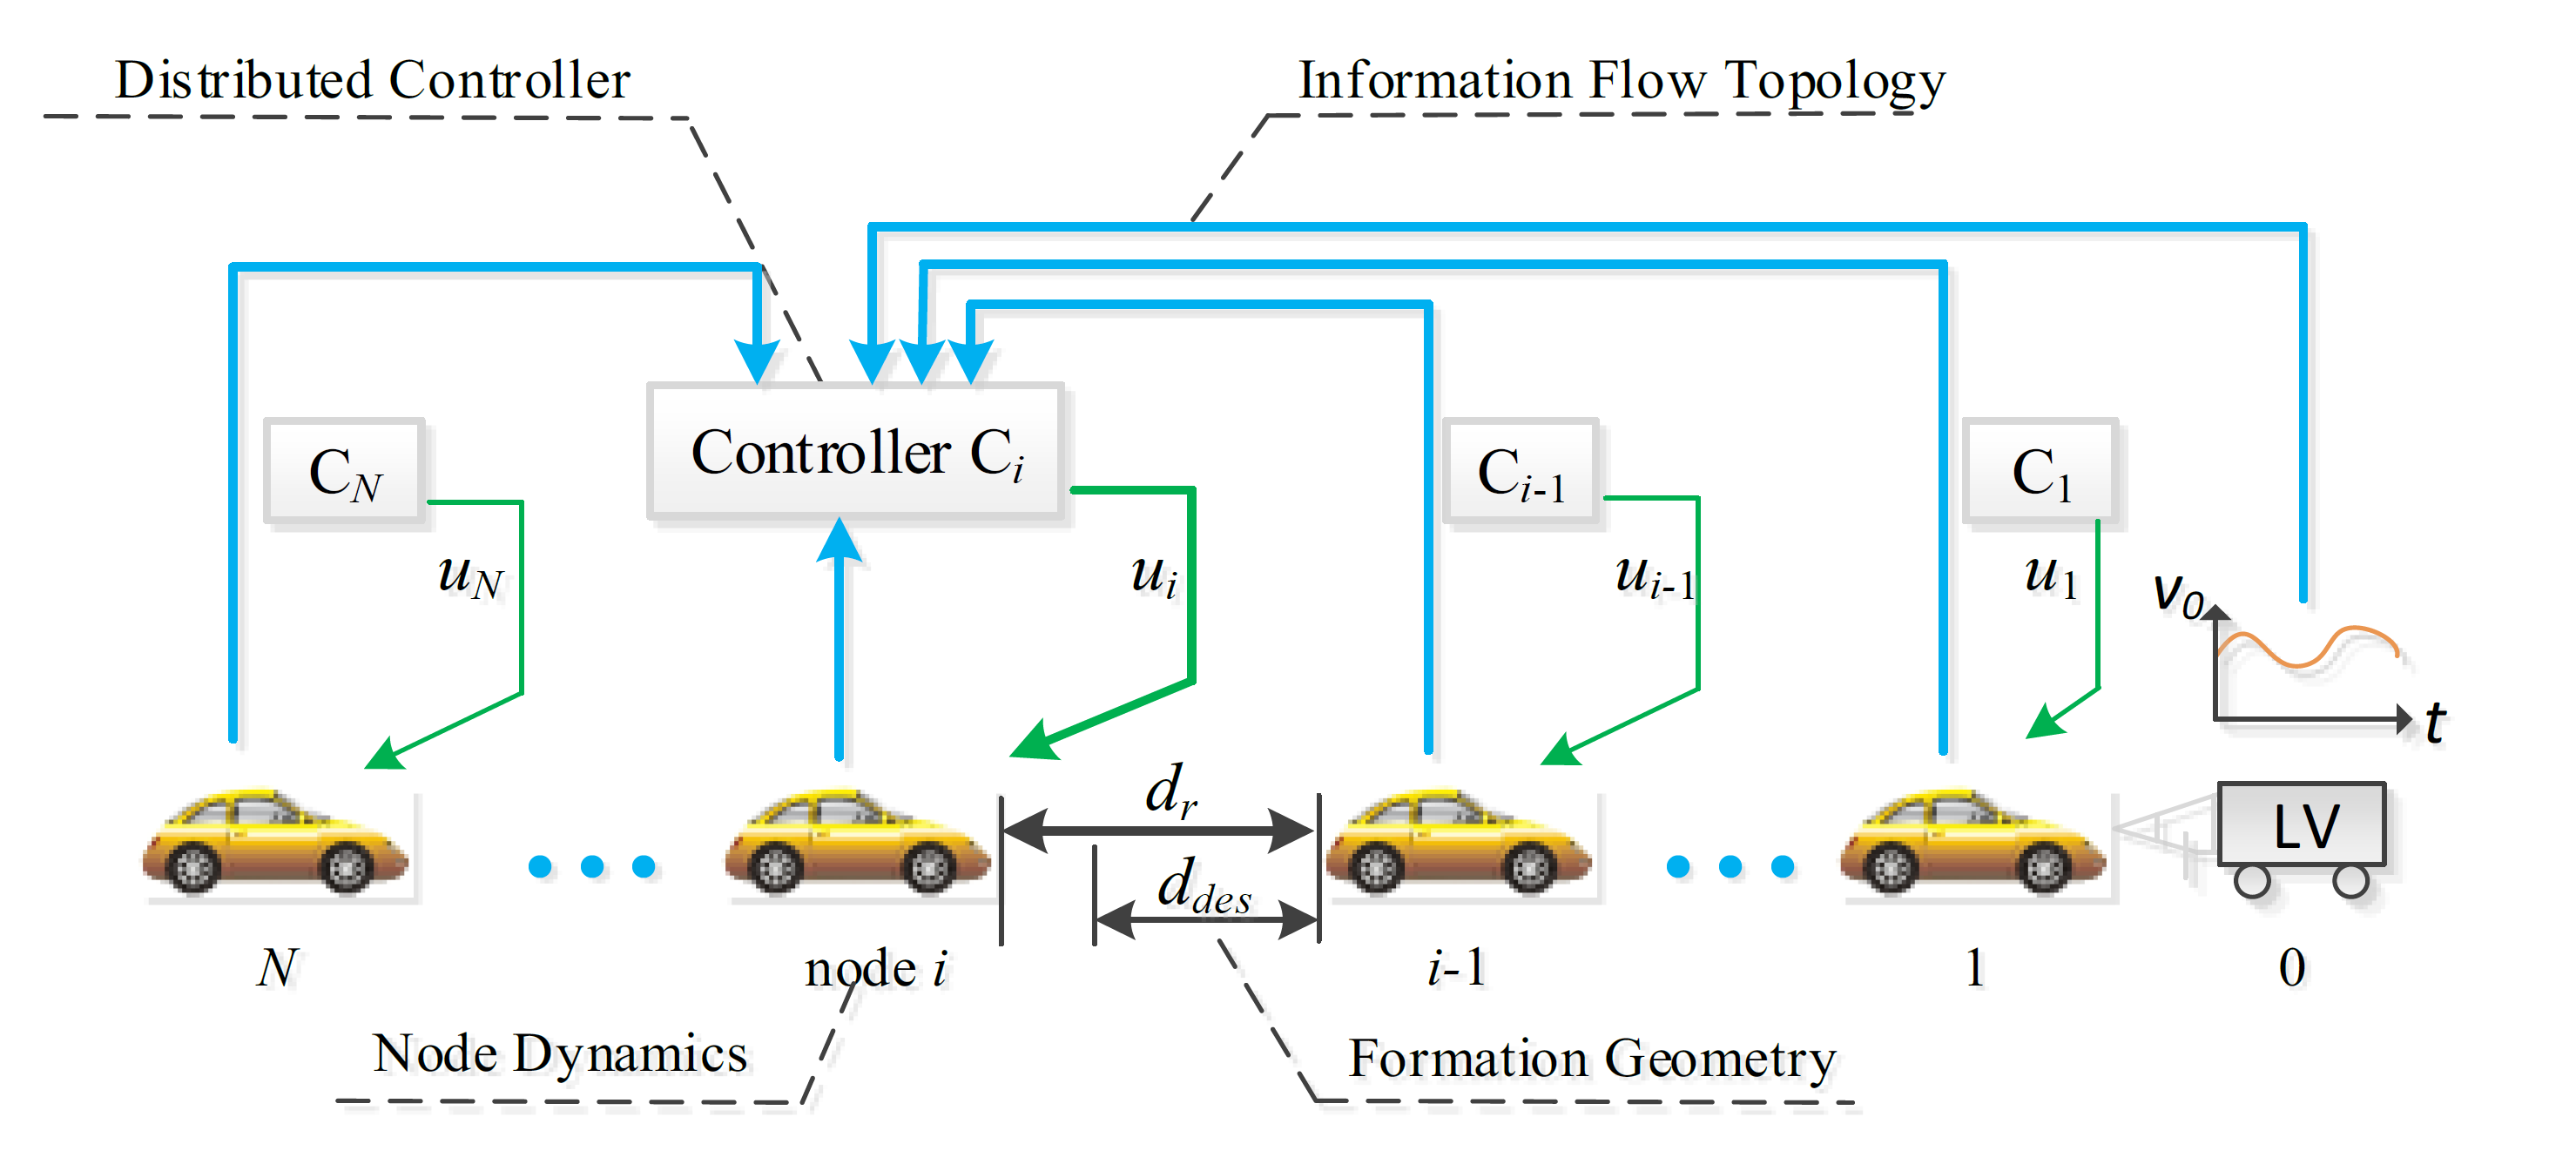
\includegraphics[scale=0.2]{Images/intro-platoon.png}
	\caption{شمای کلی از نحوه کار سیستم‌های دسته‌ای}\label{Fig intro platoon}
\end{figure}

همانطور که در شکل \ref{Fig intro platoon} مشاهده می‌شود هر ماشین باید به اندازه کافی هوشمند باشد تا بتواند موقعیت خود را بدست آورده و باید حداقل به یک یا تعداد بیشتر خودروها ارسال کند و سپس با توجه به موقعیت ارسالی از هر ماشین به کمک یک کنترلر که در هر ماشین قرار دارد به موقعیت مطلوب برسد تا آن‌ها بتوانند با هم در مسیر مطلوب حرکت کنند.

در این مقوله برای استفاده بهینه از این خودروهای خودران در بزرگراه‌ها به کنترل دسته‌ای آن‌ها روی می‌آورند. مانند شکل \ref{Fig intro platoon} به طوری که در این دسته یک رهبر\LTRfootnote{leader} و بقیه ماشین‌ها دنبال‌کننده‌ی\LTRfootnote{follower} رهبر هستند.

علاوه بر این موضوع، برنامه‌ریزی برای رسیدن به بهترین مسیر نیز یکی دیگر از نکات مهم برای حمل و نقل و خودروهای هوشمند است. منظور از برنامه‌ریزی، یافتن یک برنامه معقول برای اجرای آن است. برای مسیریابی روش‌های مختلفی همانند میدان پتانسیل\LTRfootnote{potential field}، روش نمونه‌گیری\LTRfootnote{sampling based method}، کنترل پیشبین\LTRfootnote{model predictive control}، روش‌های احتمالاتی\cite{lefkopoulos2019using} و یادگیری\LTRfootnote{learning} وجود دارند که هر کدام به طور کامل در فصل \ref{ch path planning} به طور کامل توضیح داده شده‌اند.

\section{طرح مسئله}
برای پیاده‌سازی مسئله طرح شده با هدف کنترل اجماع و مسیریابی ربات‌ها، همانطور که گفته شد از برنامه \lr{MATLAB} و \lr{mobile robotics simulation toolbox} استفاده شده است. برای تست‌های اولیه نتایج کنترل تک ربات و در انتها با 3 و 4 ربات پلتون و مسیریابی آن انجام شده است. مدل ربات‌ها به صورت دیفرانسیلی\LTRfootnote{differential} در نظر گرفته شده است که به معادلات آن در فصل \ref{ch one robot} پرداخته شده است.

اطلاعات ما از محیط از سوی دیگاه پرنده\LTRfootnote{bird's eye view} از محیط گرفته می‌شود. مسیریابی‌ها قابل برنامه‌ریزی به صورت آفلاین، با اجرای فایل \lr{.m} هر الگوریتم و سپس اجرا شبیه‌سازی مربوطه و همینطور به صورت آنلاین قابل برنامه‌ریزی است. سعی شده است که انواع روش‌های مسیریابی پیاده‌سازی و مورد بررسی قرار گیرند. همچنین تا سطح موانع متحرک، مسیریابی و کنترل اجماع به صورت بلادرنگ\LTRfootnote{real time} ارتقا یافته است.
روش‌های مسیریابی استفاده شده به شرح زیر هستند:
\begin{enumerate}
	\item میدان پتانسیل
	\item روش‌های نمونه‌برداری و ابتکاری
	\begin{itemize}
		\item \lr{BFS}\LTRfootnote{Breadth first search}
		\item \lr{Greedy best-first search}
		\item $A^*$
	\end{itemize}
	\item روش‌های یادگیری تقویتی\LTRfootnote{Reinforcement learning}
	\begin{itemize}
		\item \lr{Q-learning}
	\end{itemize}
\end{enumerate}

پیاده‌سازی این روش‌ها دارای مهارت و دانش در مورد هوش مصنوعی و روش تبدیل کردن مسئله مسیریابی برای ربات‌ها به یک مسئله دارای حالت\LTRfootnote{state}، اقدامات\LTRfootnote{actions} و تبادل اطلاعات بین ربات‌ و محیط است که در فصل \ref{ch path planning} به طور مفصل در مورد آن‌ها صحبت شده است.

نکته قابل توجه، ساده‌نویسی کد است به طوری که به راحتی بتوان آن را با زبان \lr{C} نیز درک و نوشت تا بتواند بر روی دو ربات مستقر در آزمایشگاه بلادرنگ که مدل آن‌ها نیز دیفرانسیلی است، پیاده‌سازی کرد.

\section{قالب‌بندی پایان‌نامه}























\chapter{مدل‌سازی و کنترل تک ربات‌}\label{ch one robot}
\section{مقدمه}
در این فصل چگونگی کنترل موقعیت برای هر یک از ربات‌ها توضیح داده شده است. در این پروژه از ربات‌های چرخدار دیفرانسیلی \LTRfootnote{Differential wheeled robot} استفاده شده است که ابتدا باید مدل ربات را به دست آورد. در این پروژه از مدل سینماتیکی \LTRfootnote{Kinematic model} ربات استفاده شده و وارد مدل دینامیکی نشده‌ایم. پس از توضیح مدل سینماتیکی، بر روی آن کنترل موقعیت پیاده سازی می‌شود. با توجه به مدلی که به دست آمده، می‌توان دریافت که متغیرهای کنترلی، سرعت چرخ های چپ و راست هستند و با کنترل آن‌ها و ادغام آن با سینماتیک معکوس، می‌توان کنترل موقعیت را انجام داد.

کنترل تک ربات دارای اهمیت بسیار زیادی است زیرا درون حلقه کنترل اجماع قرار می‌گیرد. حلقه داخلی باید 5 تا 10 برابر سریع‌تر از حلقه خارجی باشد تا کنترل کننده خارجی دچار مشکل نشود، در نتیجه سرعت پاسخ این کنترل کننده برای هدف نهایی بسیار اهمیت دارد.

حال که از اهمیت بالای این فصل آگاه شدیم، به بررسی نحوه بدست آوردن مدل سینماتیکی ربات‌ها می‌پردازیم.
 
\section{مدل‌سازی سینماتیکی}

در شکل \ref{Fig differential-robot} عکسی از ربات چرخدار دیفرانسیلی مشاهده می‌کنیم. 
\begin{figure}[!h]
	\centering
	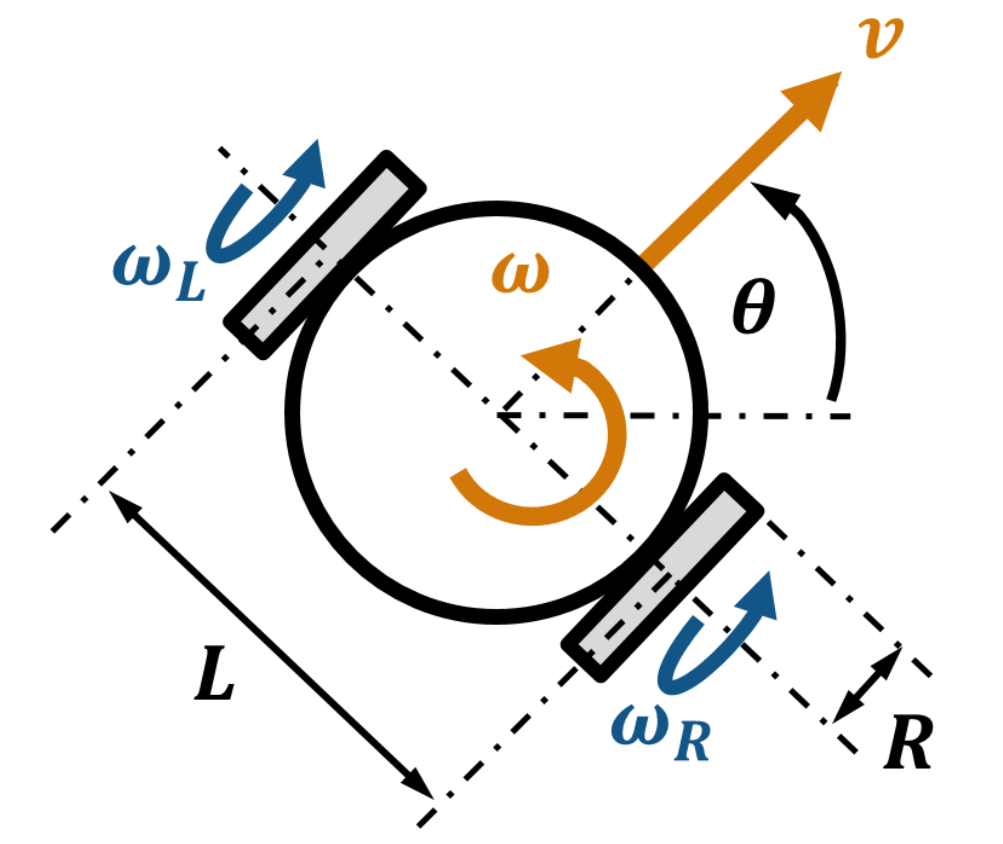
\includegraphics[scale=0.4]{Images/differential-robot-matlab.png}
	\caption{ربات استفاده شده به همراه پارامترهای آن}\label{Fig differential-robot}
\end{figure}

ورودی این ربات $\omega_L$ و $\omega_R$ که سرعت زاویه ای چرخ چپ و راست است، می‌باشد. همچنین خروجی ربات، سرعت خطی ربات، 
\verb|v|، و سرعت زاویه ای ربات، $\omega$ است. شعاع چرخ، 
\verb|R|، و فاصله بین دو چرخ، 
\verb|L|، مشخصات فیزیکی ربات هستند. در نهایت موقعیت ربات توسط مکان مرکز آن در بیان صفحه مختصات 
\verb|y|-\verb|x| و همچنین اختلاف زاویه رو به روی ربات با محور 
 \verb|x|  ها، با $\theta$ بیان می‌شود.

با توجه به شکل \ref{Fig circle-arc} اگر زاویه قطاع را $\theta$ بگیریم، داریم:
\begin{equation}
s = r\theta
\end{equation}

\begin{figure}[!h] 
	\centering
	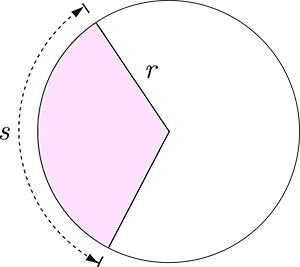
\includegraphics[scale=2]{Images/Circle_arc2.jpg}
	\caption{دایره به همراه قطاع و کمان آن} \label{Fig circle-arc}
\end{figure}

پس اگر چرح را کاملا دایره فرض کنیم و طول کمان را همچنان \verb|s| بگیریم، خواهیم داشت:
\begin{equation}
s = R\theta
\end{equation}

سپس با صرف نظر از تغییرات شعاع چرخ، به کمک یک مشتق به رابطه بین سرعت خطی و سرعت زاویه ای برای هر چرخ می‌رسیم:
\begin{equation} \label{eq wheel v w}
v = \dot{s} = R\dot{\theta} = R\omega
\end{equation}

سرعت خطی ربات با میانگین سرعت خطی هر چرخ برابر است. پس لگر سرعت خطی چرخ راست و چپ را به ترتیب با $v_{R}$ و $v_{L}$ نشان دهیم، داریم:
\begin{equation} \label{eq linear velocity}
v = \frac{v_R + v_L}{2}
\end{equation}

با ادغام روابط \ref{eq wheel v w} و \ref{eq linear velocity} داریم:
\begin{equation} \label{eq forward kinematics v}
v = \frac{R}{2}(\omega_R + \omega_L)
\end{equation}

برای محاسبه سرعت زاویه ای ربات از \verb|ICC| \LTRfootnote{Instantaneous center of curvature} استفاده می‌شود که ربات همانند شکل \ref{Fig differential-robot-ICC} حول آن دوران می‌کند. قابل توجه است که چون دو چرخ آخر خودرو آزادی عمل ندارند، می توان خودرو را با ربات چرخدار دیفرانسیلی مدل کرد.
\begin{figure}[!h] 
	\centering
	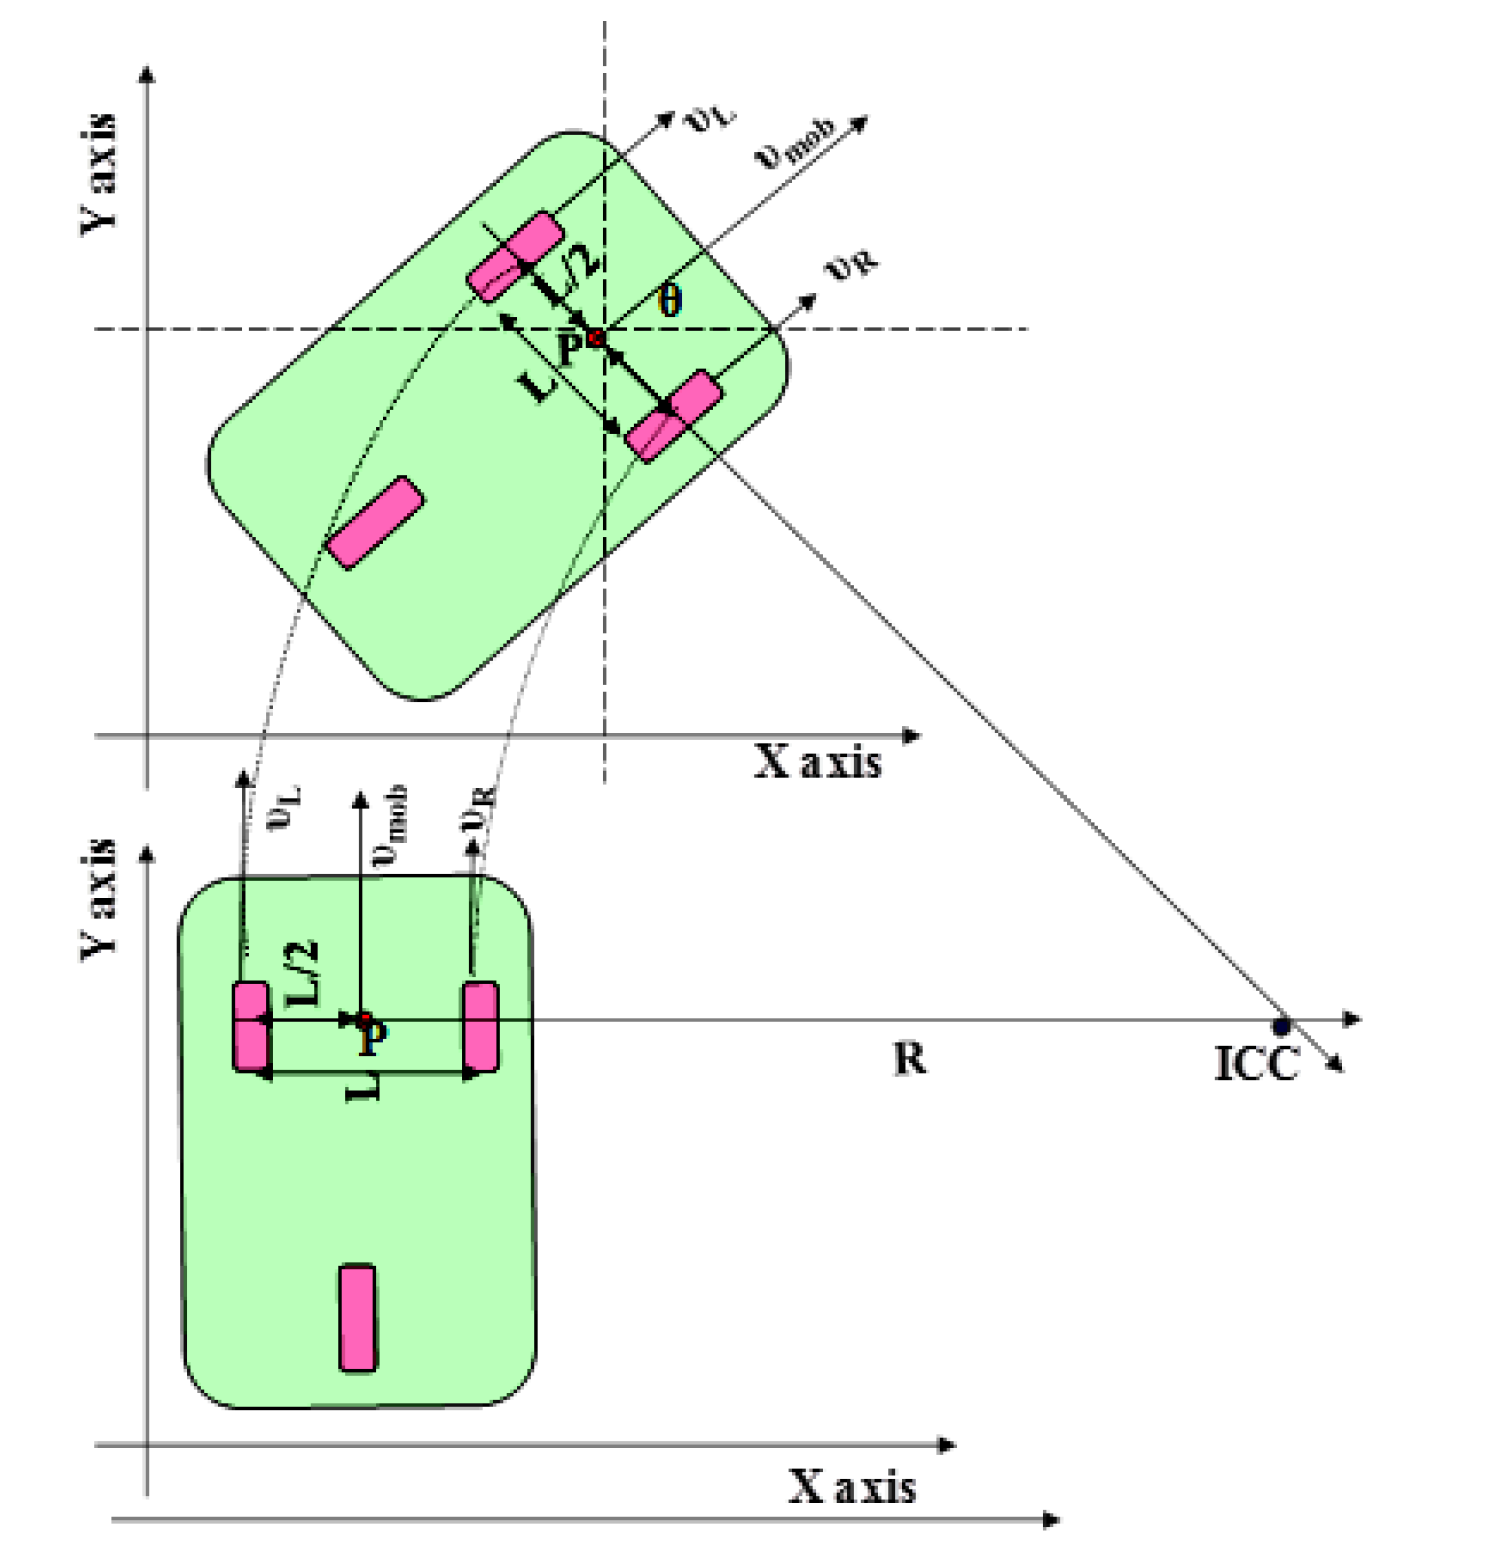
\includegraphics[scale=0.28]{Images/differential-robot-ICC.png}
	\caption{چرخش ماشین حول یک نقطه مشخص} \label{Fig differential-robot-ICC}
\end{figure}

مقدار \verb|ICC| طبق رابطه زیر به دست می‌آید:
\begin{equation}
ICC = (x - Rsin(\theta), y + Rcos(\theta))
\end{equation}
 که \verb|R| فاصله بین مرکز دو چرخ جلوی خودرو و نقطه‌ای است که حول آن دوران می‌کند. پس داریم:
 
\begin{equation} \label{eq ICC radius}
R = \frac{L}{2} \times \frac{v_L + v_R}{v_L - v_R}
\end{equation}

حال اگر دایره را به مرکز \verb|ICC| و شعاع \verb|R| در نظر بگیریم، با توجه به روابط \ref{eq wheel v w}، \ref{eq linear velocity} و \ref{eq ICC radius} داریم:
\begin{equation} \label{eq forward kinematics w}
\omega = \frac{v}{R} = \frac{R}{L}(v_R - v_L)
\end{equation}

در نتیجه با توجه به معادلات \ref{eq forward kinematics v} و \ref{eq forward kinematics w}، سینماتیک معکوس ربات برابر است با:
\begin{equation} \label{eq inverse kinematics}
\omega_L = \frac{1}{R}(v - \frac{\omega L}{2}),~~~  \omega_R = \frac{1}{R}(v + \frac{\omega L}{2})
\end{equation}

حال اگر در کنترل کننده موقعیت، مقدار \verb|v| و $\omega$ را محاسبه کرد، می‌توان به کمک رابطه \ref{eq inverse kinematics} سرعت زاویه‌ای چرخ‌ها را طوری تنظیم نمود که ربات به سرعت خطی و زاویه‌ای ایده‌آل خود برسد.

\section{کنترل کننده موقعیت تک ربات}

در این قسمت هدف این است که موقعیت ربات، یا به عبارتی مختصات مرکز ربات را در صفحه \verb|y|-\verb|x| کنترل کرد. متغیر کنترلی، سرعت زاویه‌ای چرخ‌ها می باشد. حال هدف این است که با محاسبه خطا و به کمک کنترل کننده، خروجی کنترل کننده را به سرعت خطی و زاویه‌ای ربات تبدیل کنیم تا در نهایت با کمک از رابطه سینماتیک معکوس \ref{eq inverse kinematics} بتوان به سرعت زاویه‌ای چرخ‌ها رسید.

\subsection{کنترل سرعت زاویه‌ای ربات}
در این کنترل ‌کننده هدف ما این است که سر ربات به سمت موقعیت مرجع باشد. در نتیجه پس از محاسبه خطا داریم:
\begin{equation}
e = 
\begin{bmatrix}
x_d - x \\
y_d - y
\end{bmatrix}
\end{equation}

که در آن $x_d$ و $y_d$ موقعیت مرجع و \verb|x| و \verb|y| موقعیت فعلی ربات هستند.

حال با توجه به خطای به دست آمده، با کمک از تابع \verb|Atan2| زاویه‌ای که ربات باید در آن جهت قرار بگیرد، محاسبه می‌گردد. مزیت استفاده از این تابع این است که برد آن در بازه
$-\pi$
تا
$\pi$
می‌باشد و باعث می‌شود که جهت رو‌به‌روی ربات اهمیت پیدا کند. قابل ذکر است که اگر از \verb|arctan| استفاده می‌شد، آنگاه فقط راستای رو‌به‌روی ربات اهمیت پیدا می‌کرد و برای حالتی که ربات رو به نقطه مرجع یا پشت به آن می‌باشد، فرقی قائل نمی‌شد.

در شکل \ref{Fig atan2} دامنه و برد تابع \verb|Atan2| قابل مشاهده است.
\begin{figure}[!h] 
	\centering
	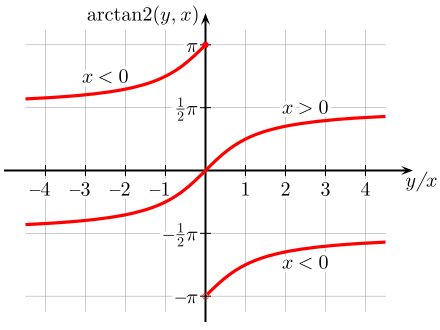
\includegraphics[scale=0.8]{Images/atan2.png}
	\caption{دامنه و برد تابع استفاده شده} \label{Fig atan2}
\end{figure}

اکنون با کمک این تابع زاویه‌ای که ربات باید در آن جهت قرار گیرد، $\theta_d$، به صورت زیر محاسبه می‌گردد:
\begin{equation}
\theta_d = Atan2(y_d - y, x_d - x)
\end{equation}
که ورودی‌های تابع، عناصر بردار خطا هستند.

حال که زاویه مرجع به دست آمد، با کم کردن زاویه حال حاضر ربات، به خطای زاویه می‌رسیم. سپس با استفاده از کنترل کننده انتگرال‌گیر نسبت، به سرعت زاویه‌ای ربات دست پیدا می‌کنیم. در نتیجه با تنظیم سرعت زاویه‌ای چرخ‌ها به طوری که به سرعت زاویه‌ای مد نظر در ربات برسیم، می‌توان چهت‌گیری ربات را کنترل نمود. در قسمت بعد، به چگونگی کنترل سرعت خطی ربات پرداخته خواهد شد. 

\subsection{کنترل سرعت خطی ربات}
برای کنترل سرعت خطی ربات، فاصله بین مکان حال تا موفعیت هدف، به عنوان ورودی کنترلی مد نظر قرار می‌گیرد. قابل ذکر است که این فاصله برابر با نرم دو بردار اختلاف این دو موقعیت است و از این رابطه در کنترل استفاده شده است. در نتیجه ورودی کنترلی برابر است با:
\begin{equation}
\|e\|_2 = \sqrt{(x_d - x)^{2} + (y_d - y)^{2}}
\end{equation}

در این قسمت از کنترل کننده نسبت مشتق‌گیر\LTRfootnote{PD} استفاده شده است. دلیل استفاده نیز این بود که سرعت ربات دارای اهمیت است، در نتیجه از انتگرال‌گیر که سرعت را کاهش می‌دهد، استفاده نشده است. ار طرفی چون پاسخ گذرا هنگام کنترل سرعت دارای اهمیت است، از مشتق‌گیر استفاده شده است تا پاسخ را بهبود بخشد. همچنین برای جلوگیری از وارد شدن ولتاژ بیش از حد به ربات، در خروجی کنترلی اشباع قرار داده شده است تا سرعتی که از ربات می خواهیم و در نتیجه ولتاژ اعمالی به موتور چرخ ها، محدود گردد.

\subsection{کنترل کننده خاموش روشن}
برای کاهش تاثیر نویز، قبل از کنترل‌کننده سرعت و زاویه، از کنترل‌کننده خاموش روشن با بازه 0/3 استفاده شده است. علاوه بر این در کنترل‌کننده سرعت از مقدار خروجی در حالت قبل نیز فیدبک گرفته شده است. دلیل این کار این است که ربات در حدود فاصله تعیین شده می‌ایستاد و نسبت به نویز با مقدار بسیار کم نیز حساس می‌ماند. با بررسی خروجی گذشته با اینکه به مقدار کمتر از 0/05 رسیده باشد، خیالمان راحت خواهد شد زمانی سرعت صفر خواهد شد، که بسیار به موقعبت مطلوب نزدیک شده باشیم. و در نتیجه به نویز در حدود 0/3 نیز مقاوم خواهیم بود.

حال نتایج آزمایشات برای یک ربات، مورد بررسی قرار می‌گیرد.

\section{نتایج کنترل موقعیت یک ربات}
کنترل‌کننده تک ربات در شکل \ref{Fig 1-robot-controller} آمده است. در قسمت بنفش‌رنگ بلوک‌های کنترلی به طور خاص مشخص شده‌اند.
\begin{figure}[!h] 
	\centering
 	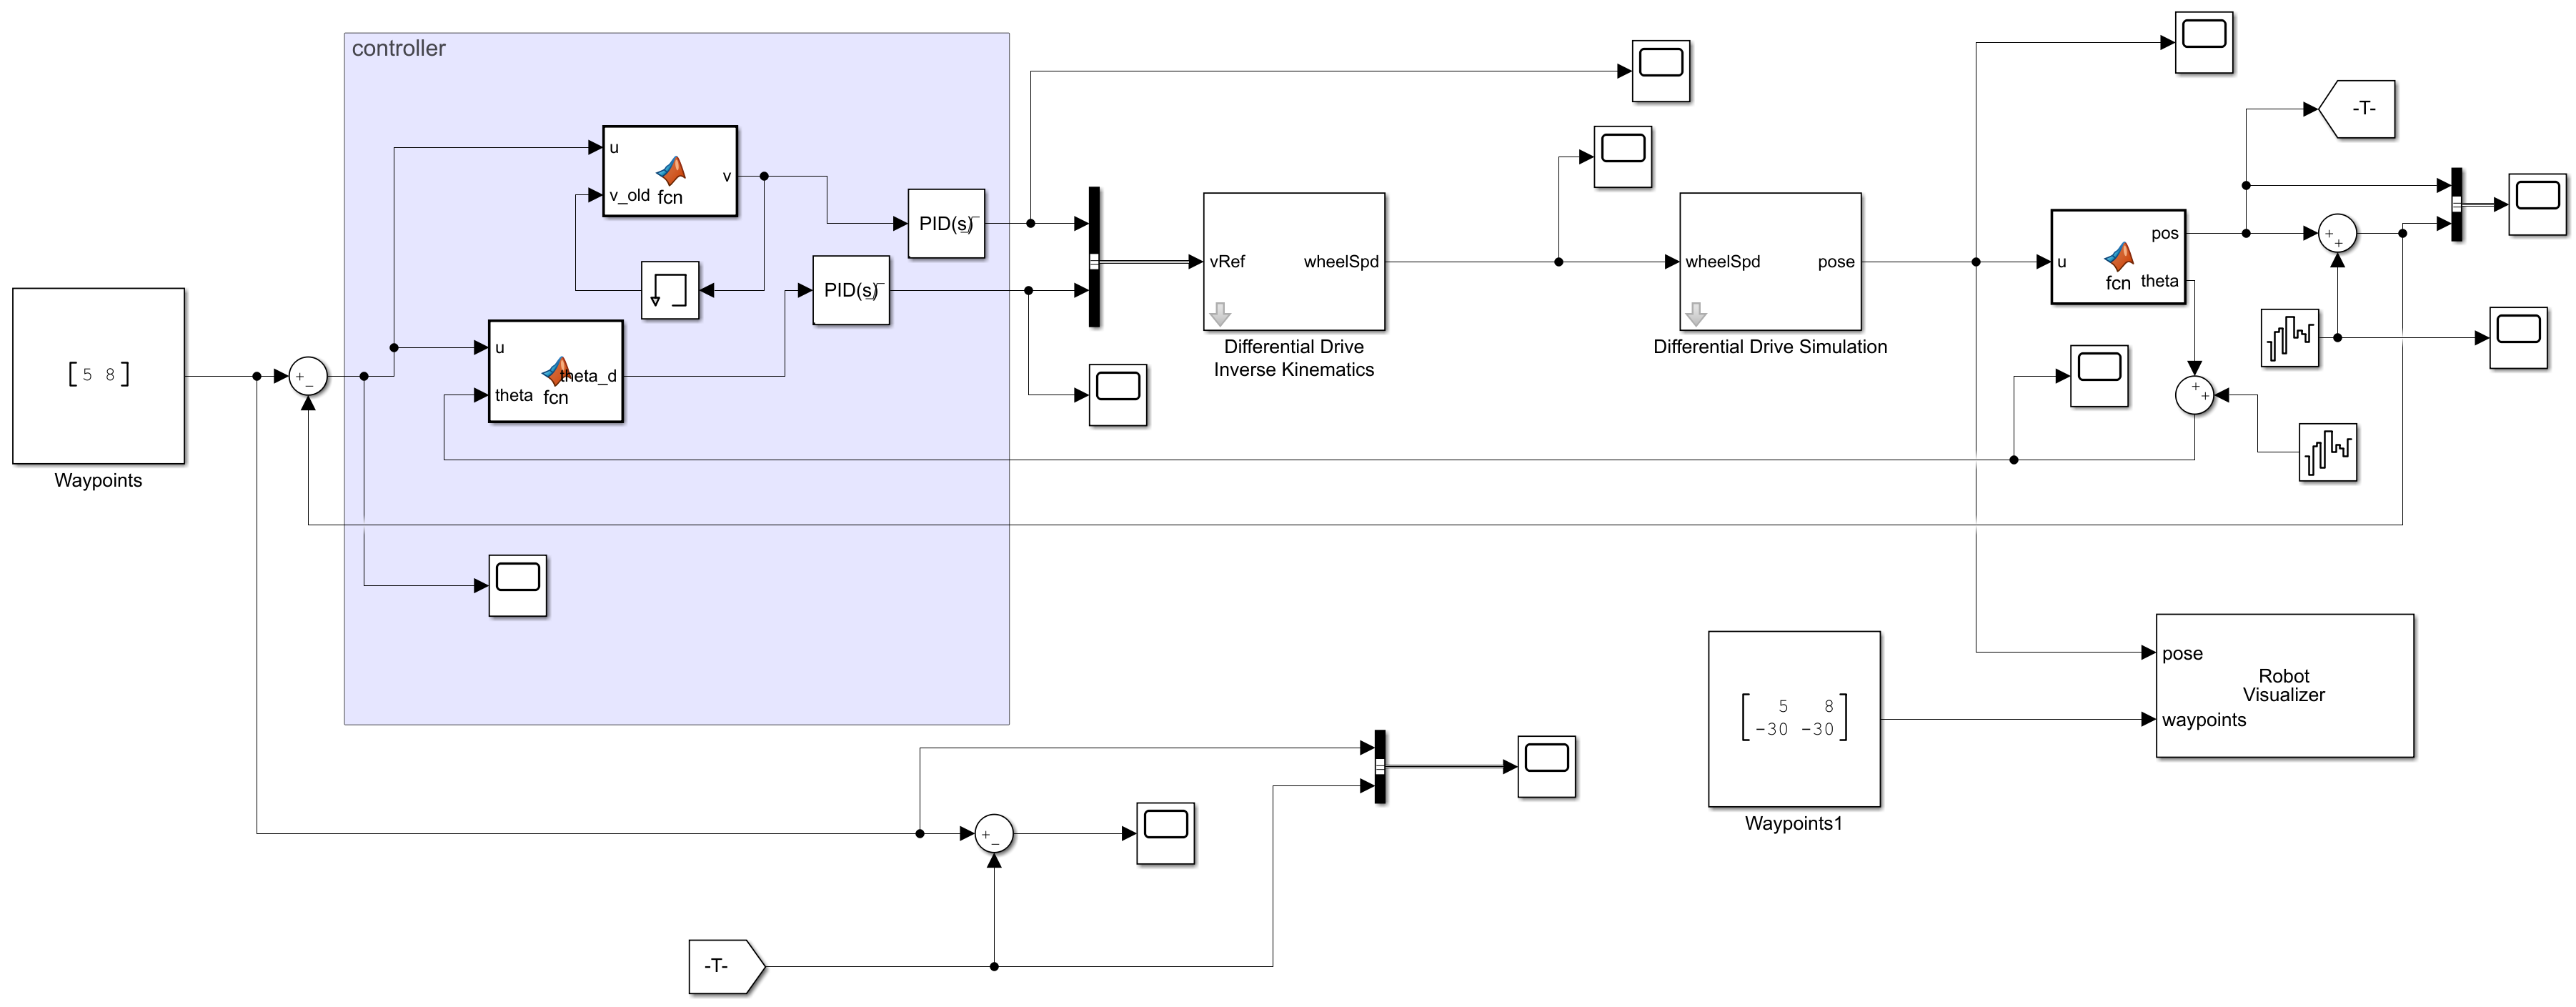
\includegraphics[scale=0.16]{Images/1-robot controller.png}
	\caption{کنترل‌کننده تک ربات} \label{Fig 1-robot-controller}
\end{figure}
 
 در کنترل سرعت، کنترل‌کننده نسبت با $P=1$ پیاده‌سازی شده است. در کنترل‌کننده زاویه، کنترل‌کننده نسبت با $P=10$ برای سرعت بیشتر به دلیل اینکه اول باید زاویه درست شود استفاده شده است.
 
 نویز استفاده شده به صورت تابع احتمال گاوسی، و با بیشترین خطای 0/1 متر به سنسورها اعمال شده است. موقعیت اولیه برابر $[15~~14]^T$ و موقعیت مطلوب برابر $[5~~8]^T$ بوده است.
 
در نمودار \ref{Fig 1-robot-pos} موقعیت واقعی ربات و موقعیت مطلوب، نمایش داده شده است. که نشان از تعقیب مناسب نقطه مطلوب توسط ربات است.
 \begin{figure}[!h] 
 	\centering
 	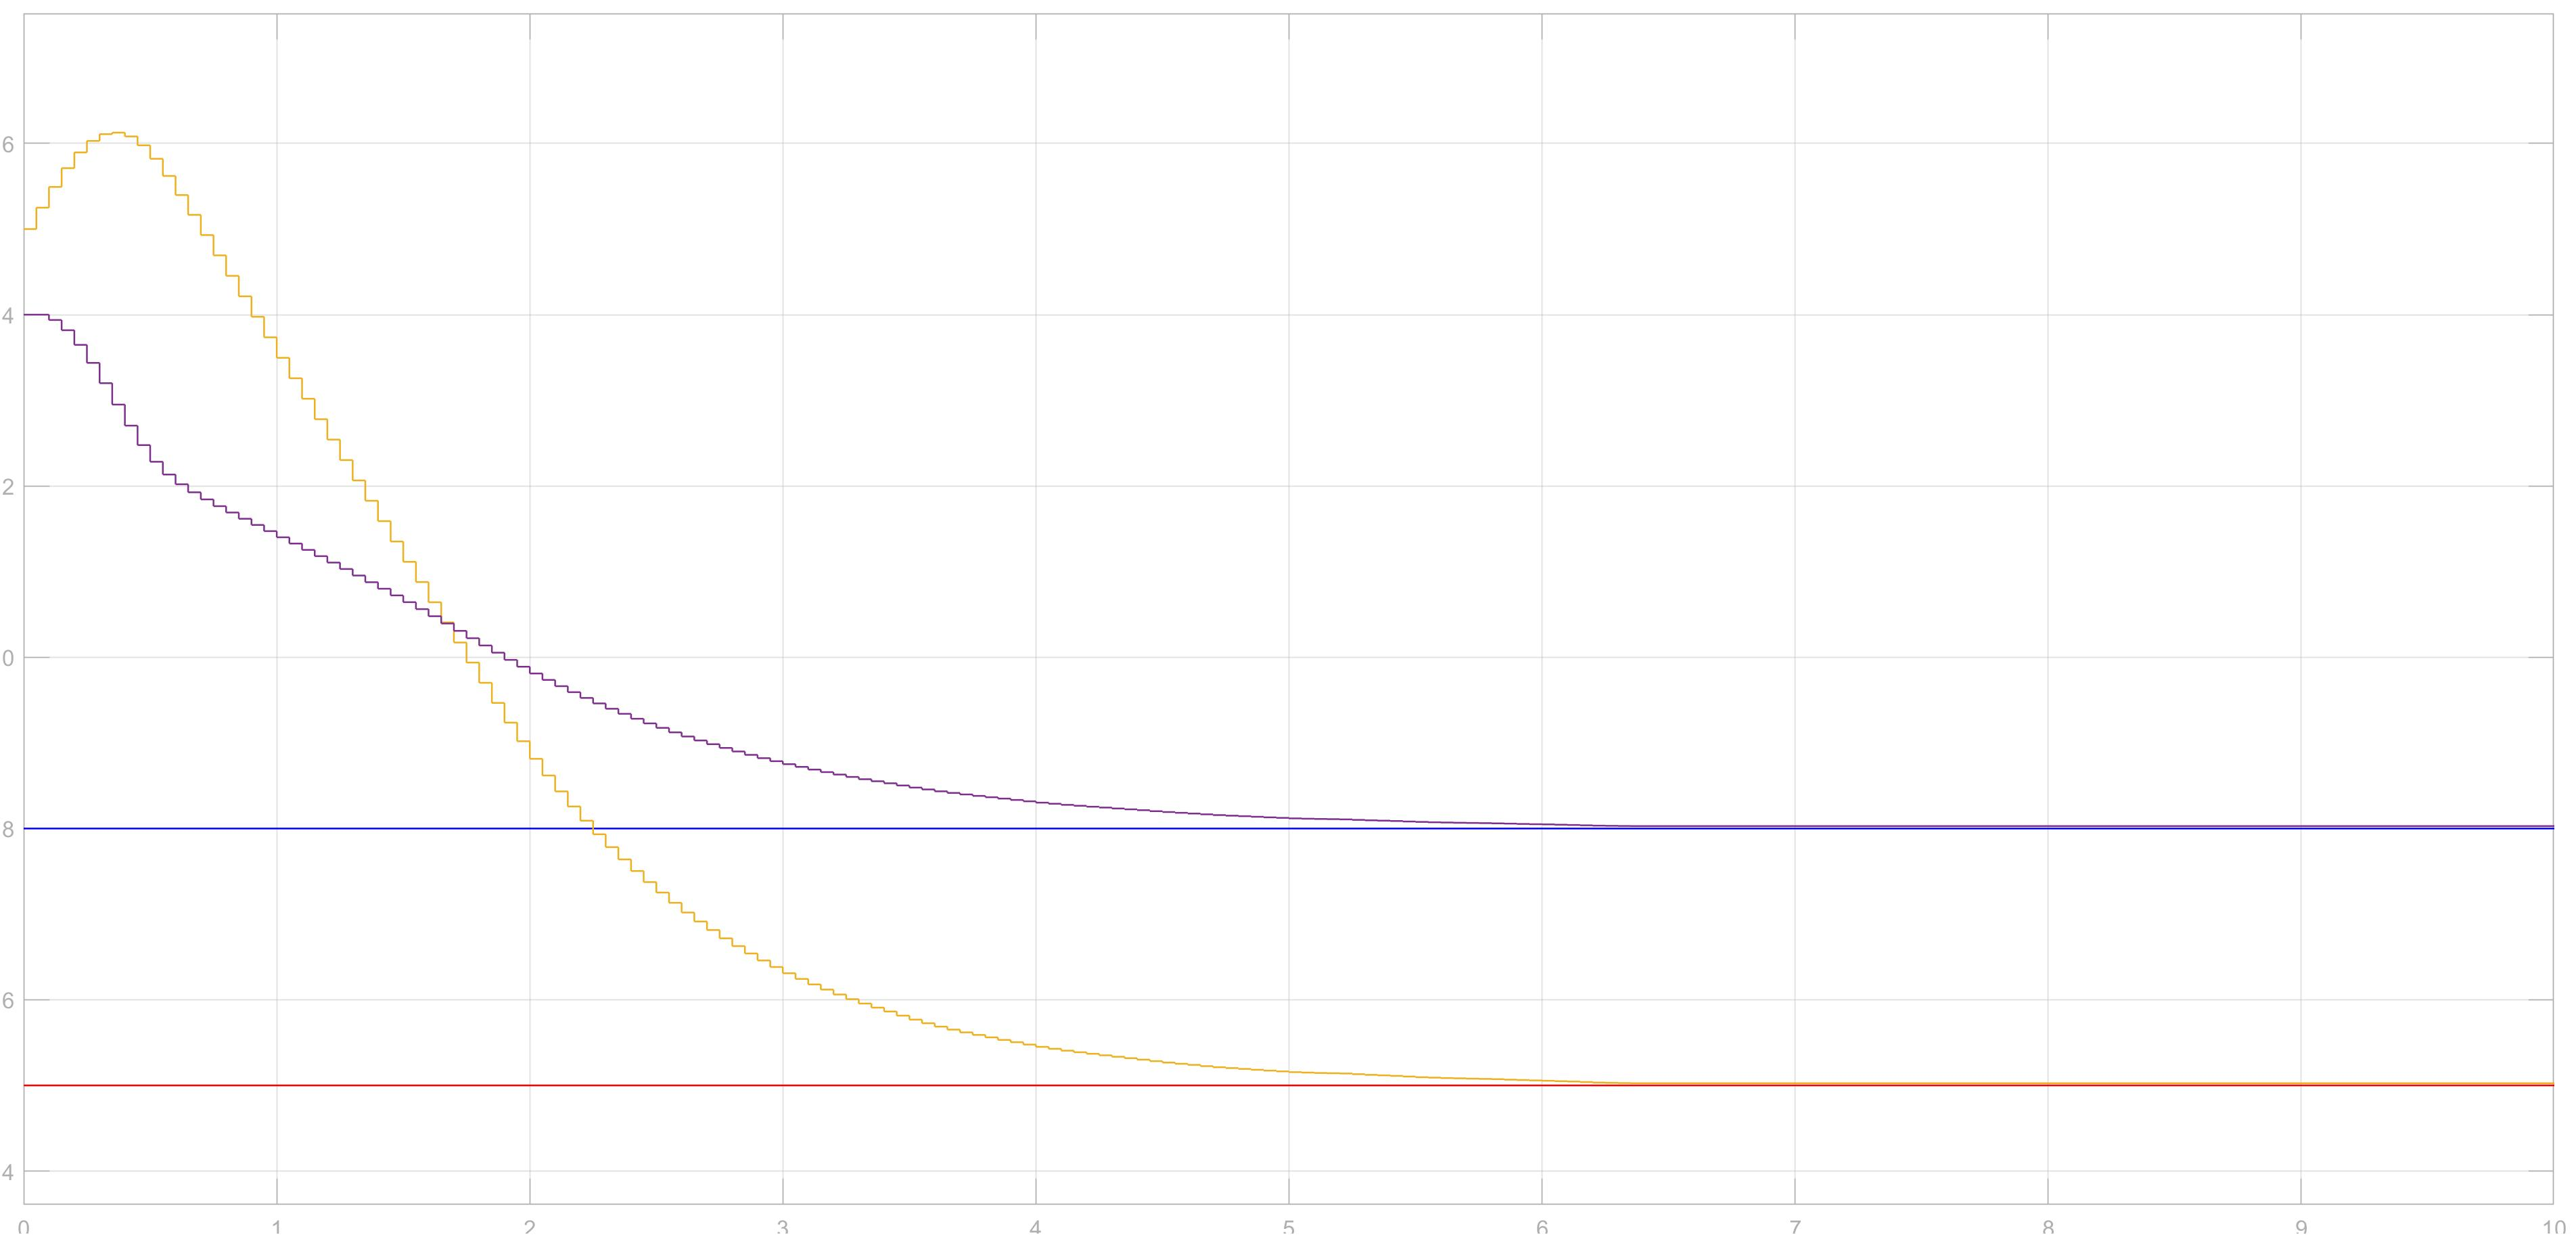
\includegraphics[scale=0.12]{Images/1-robot pos.jpg}
 	\caption{موقعیت مطلوب و موقعیت واقعی ربات} \label{Fig 1-robot-pos}
 \end{figure}
 
 شکل‌های \ref{Fig 1-robot-noise}، \ref{Fig 1-robot-speed} و \ref{Fig 1-robot-motors} نیز نشان‌دهنده سرعت زاویه‌ای چرخ‌ها پس از رسیدن به هدف و حذف اثر نویز و محدود بودن سرعت خطی ربات هستند.
 
 \begin{figure}[!h] 
 	\centering
 	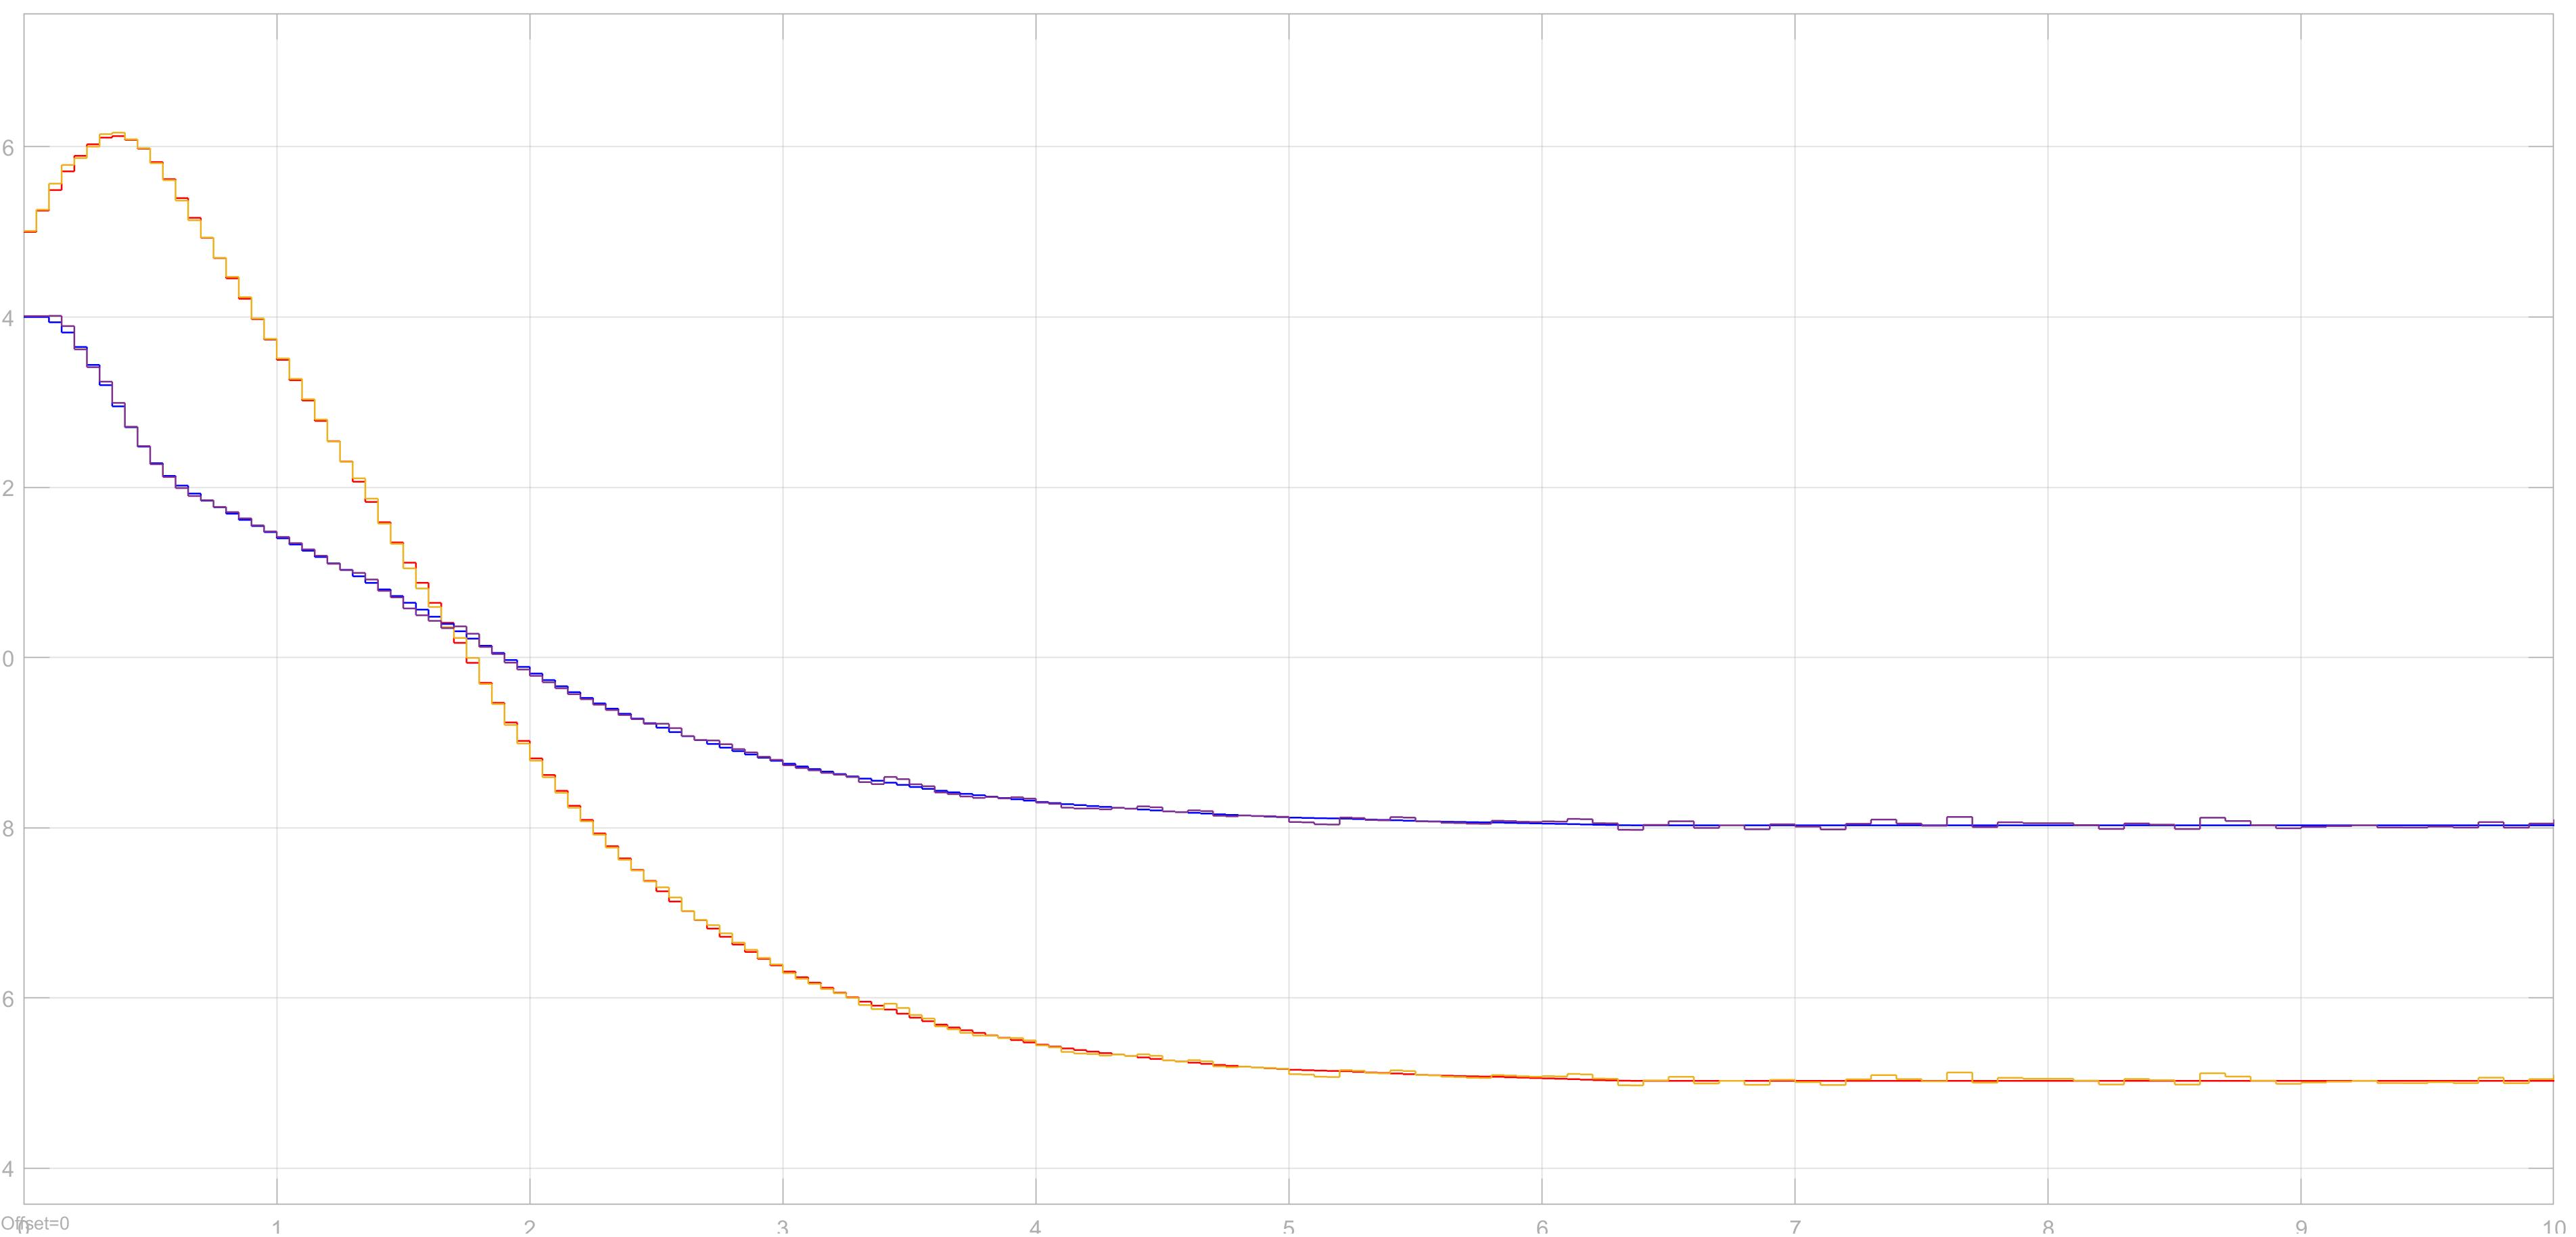
\includegraphics[scale=0.12]{Images/1-robot noise.jpg}
 	\caption{موقعیت واقعی و موقعیت فیدبک گرفته شده از سنسور ربات} \label{Fig 1-robot-noise}
 \end{figure}
 
 \begin{figure}[!h] 
 	\centering
 	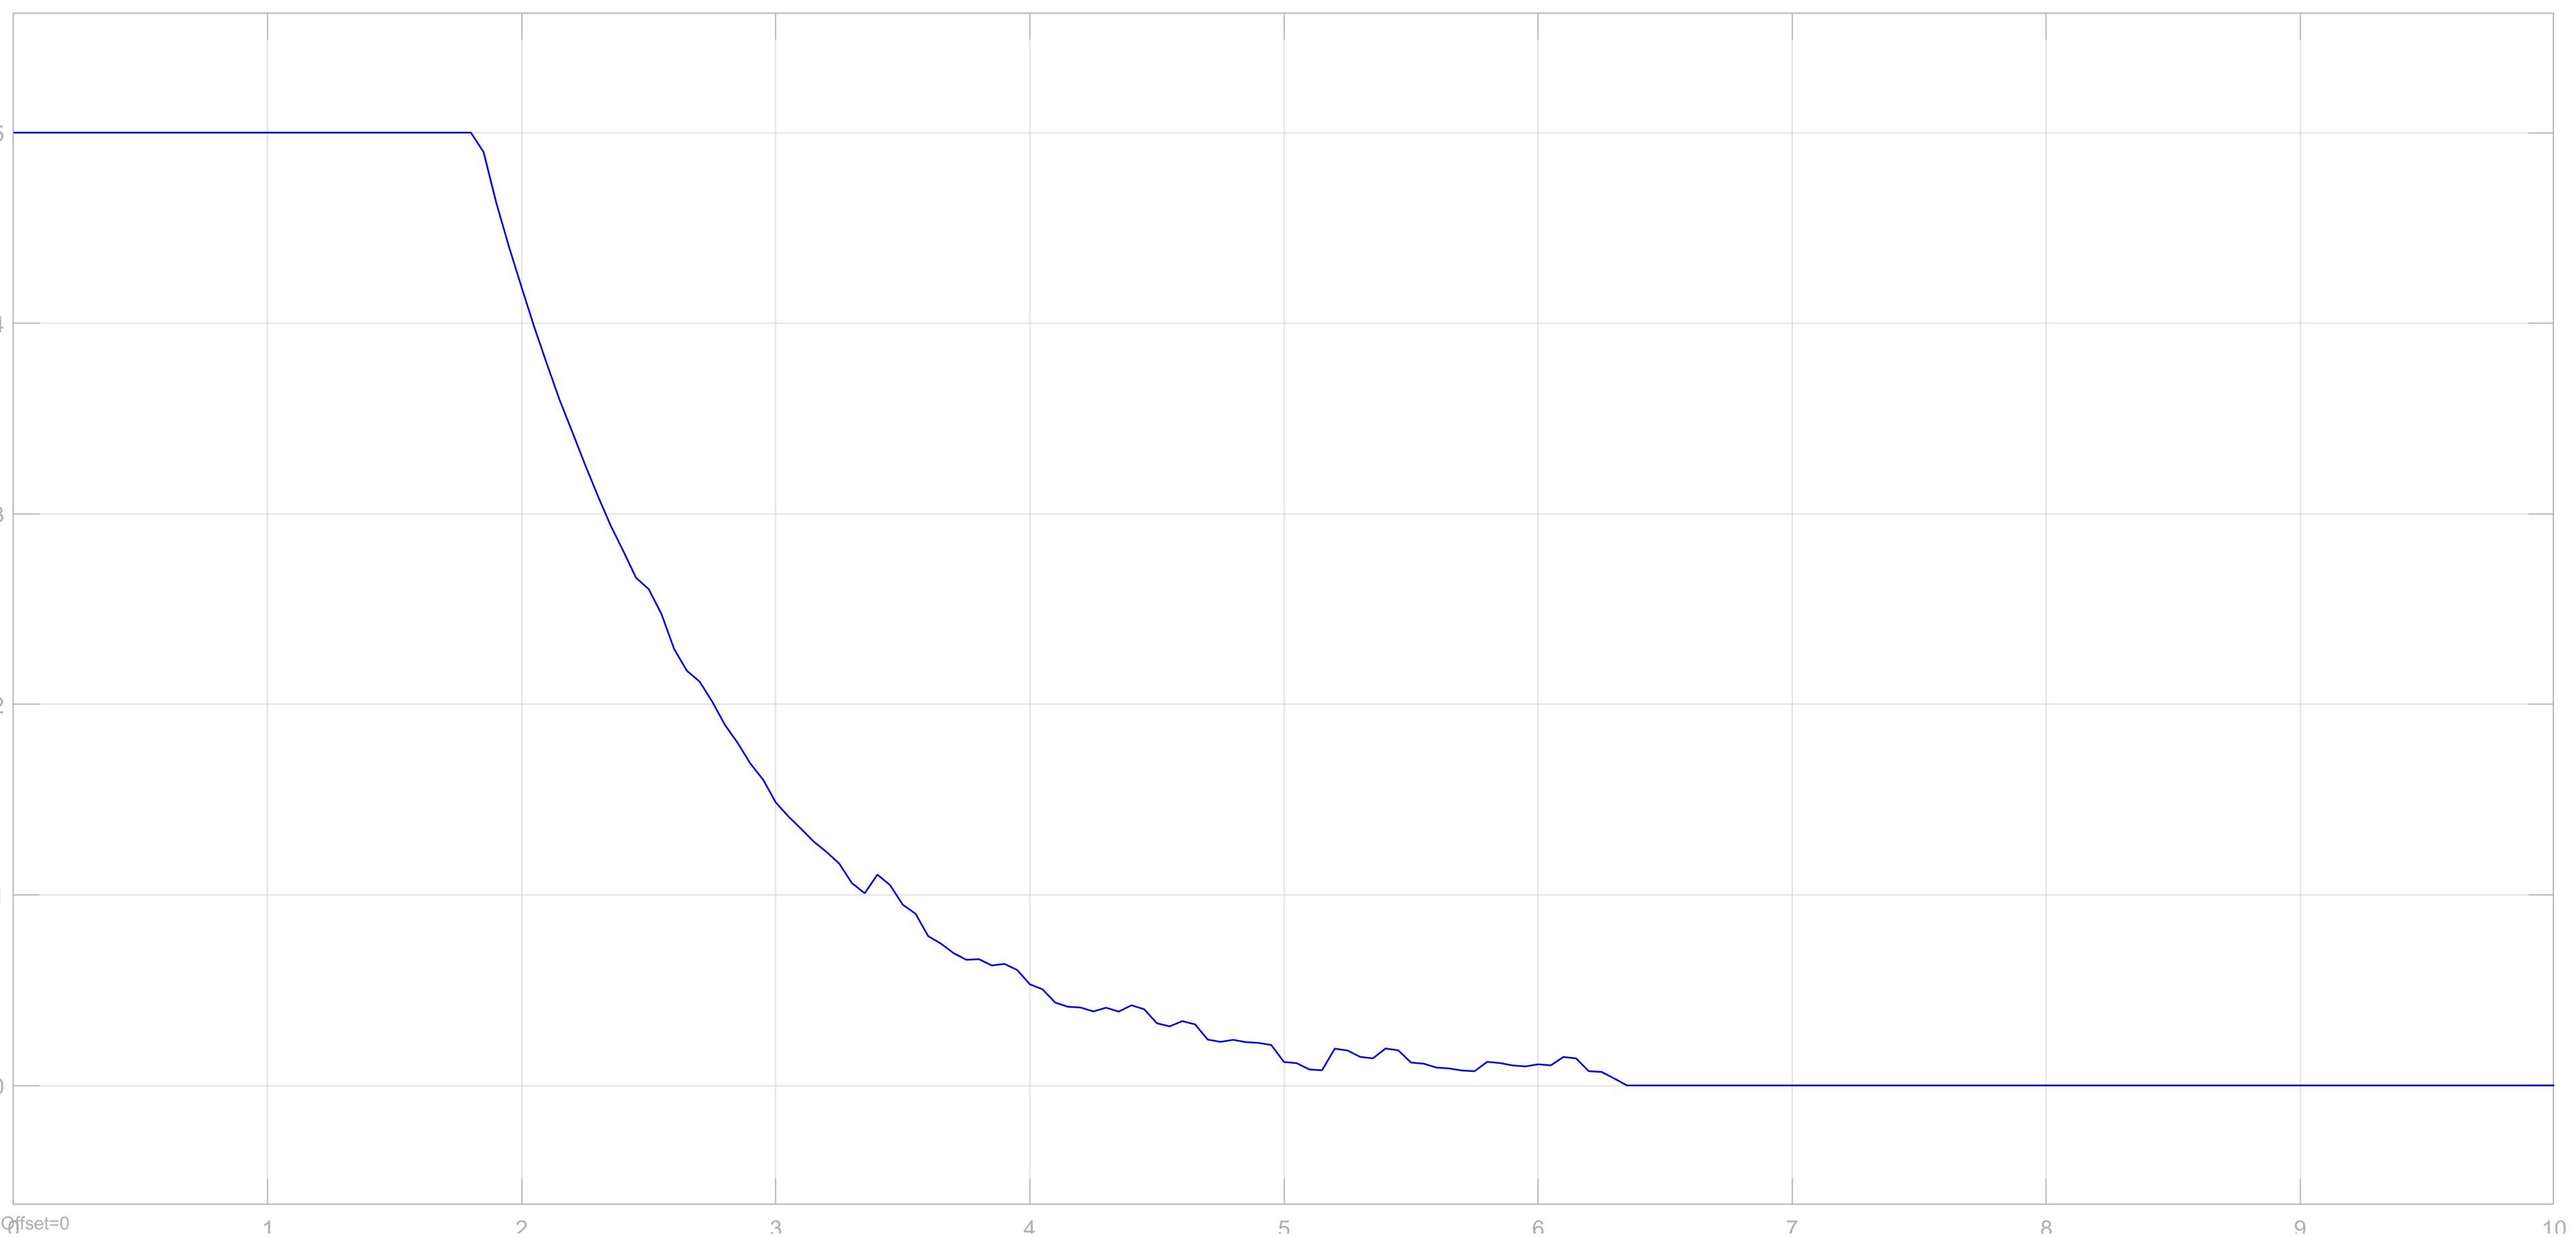
\includegraphics[scale=0.12]{Images/1-robot speed.jpg}
 	\caption{سرعت خطی ربات} \label{Fig 1-robot-speed}
 \end{figure}
 
 \begin{figure}[!h] 
 	\centering
 	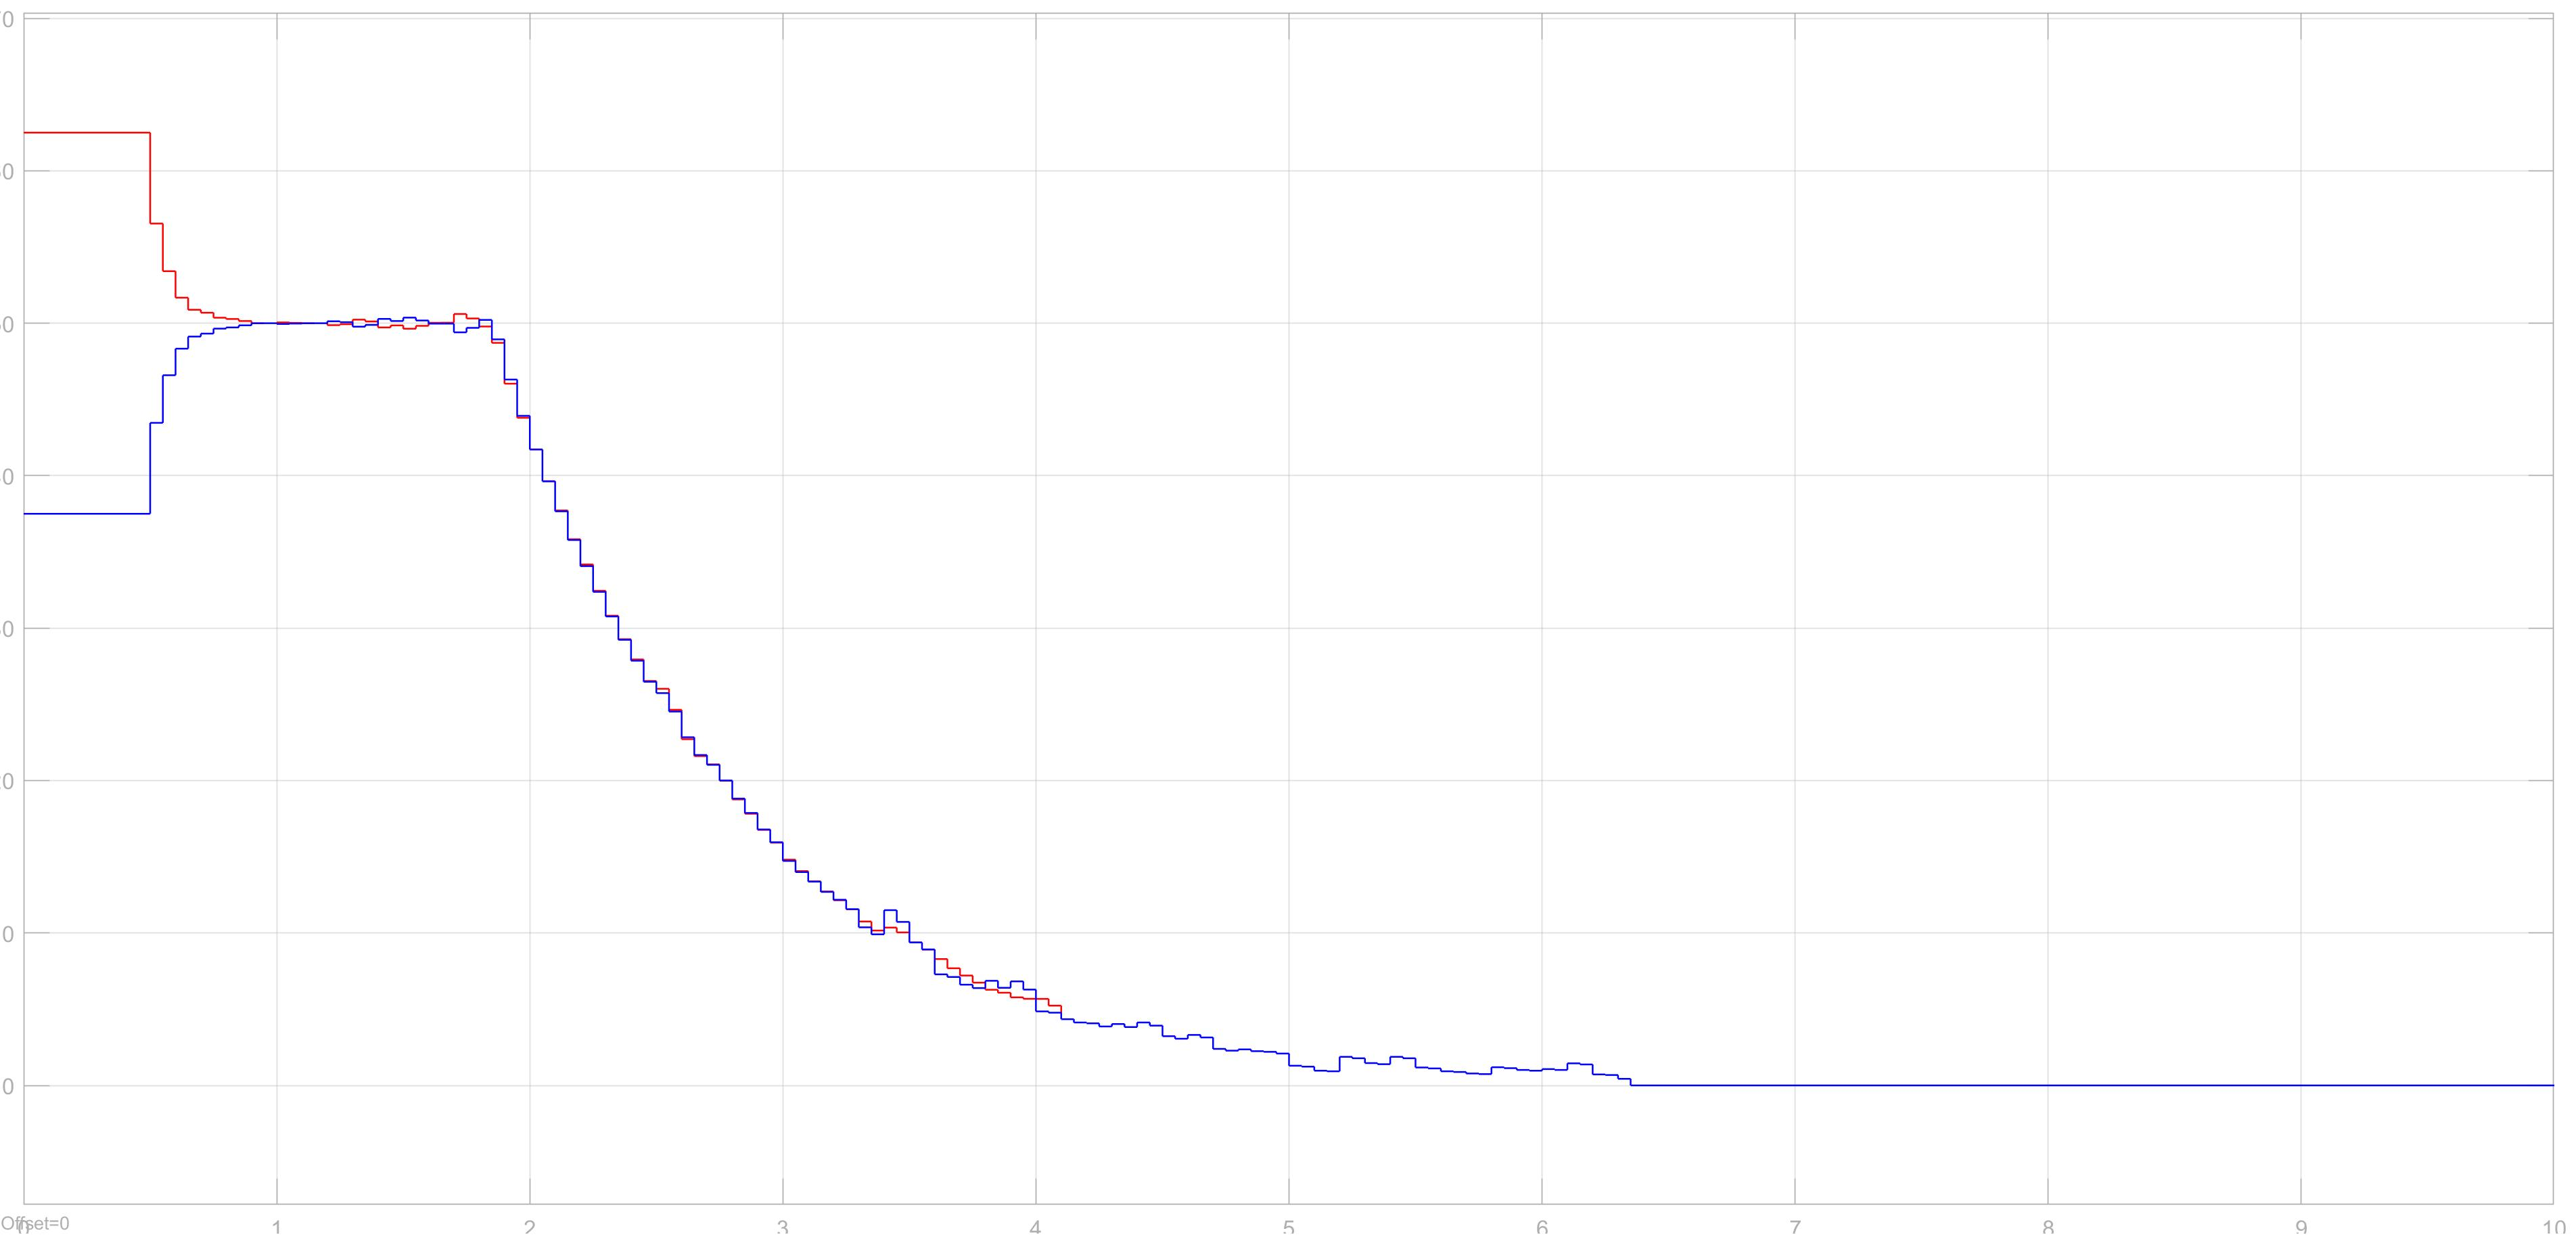
\includegraphics[scale=0.12]{Images/1-robot motors.jpg}
 	\caption{سرعت زاویه‌ای چرخ‌های ربات} \label{Fig 1-robot-motors}
 \end{figure}
 
 
 
 
 
 
 
 
 
 
 
 
\chapter{کنترل اجماع ربات‌‌ها}
%\thispagestyle{empty}

\section{مقدمه}
این فصل را می‌توان مهم‌ترین بخش این پروژه دانست که هدف آن کنترل سیستم‌های چند عاملی\LTRfootnote{Multi-agent systems} به صورت دسته‌ای\LTRfootnote{Platoon} از ربات‌هاست، به طوری که رهبر\LTRfootnote{Leader} دسته را دنبال کنند. در ادبیات سیستم‌های چند عاملی به هر خودرو یا ربات، عامل گفته می‌شود. همچنین همانطور که در ادامه خواهیم دید، یک خودرو فرضی نیز می‌تواند به عنوان رهبر در نظر گرفته شود. در سیستم‌های چند عاملی، هر عامل با داشتن اطلاعات عامل‌های دیگر، که می‌تواند بین یک تا تمام عامل‌های دیگر باشد، رهبر را دنبال می‌کند. در نتیجه، تمامی عامل‌ها درباره اینکه رهبر در کجا قرار دارد به اجماع\LTRfootnote{Consensus} برسند. به همین دلیل به الگوریتم‌های انجام دهنده این عمل، الگوریتم اجماع می‌گویند.

الگوریتم‌های اجماع تحت تاثیر ارتباطات بین عامل‌ها هستند و می‌توان با توجه به اینکه کدام ربات‌ها با هم داده تبادل می‌کنند، گراف ساده جهت‌داری\LTRfootnote{Simple directed graph} رسم نمود. به این منظور هر عامل را به یک راس\LTRfootnote{Vertex} و هر ارتباط را یک یال\LTRfootnote{Edge} جهت‌دار که از عامل فرستنده یال خارج و به عامل گیرنده وارد می‌شود، نسبت داد. همچنین، دور به طول‌ یک، یالی که از یک راس به خودش وارد می‌شود، و تعداد بیشتر از یک یال بین دو راس مشخص وجود ندارد. هر گراف را می‌توان به نحوه‌های مختلفی، همچون ماتریس مجاورت\LTRfootnote{Adjacency matrix} و لیست مجاورت\LTRfootnote{Adjacency list} نمایش داد. در پروژه با توجه به ادامه کار و نیازمان، از ماتریس مجاورت استفاده شده است که دلیل آن را در ادامه خواهیم دید.

\section{گراف اجماع}
گراف اجماع تاثیر بسیار زیادی بر پروژه و عملکرد آن دارد. هر یال (ارتباط)، به دلیل اضافه کردن محاسبات، شامل هزینه زمانی است و باعث بیشتر شدن زمان نمونه برداری می‌شود. از طرفی در صورت قطعی موقت ارتباط، نباید عامل ارتباط خود با دسته را به طور کامل از دست ندهد. در نتیجه مبحثی که پیش می‌آید این است که گرافی را طوری طراحی کنیم که در صورت قطع یک سری از ارتباطات تضمین شود هیچ عاملی ارتباطش را با دسته از دست نمی‌دهد. در این راستا از مباحث نظریه گراف بهره می‌بریم.

\subsection{عدد همبندی یالی}\label{se edge connectivity}

 در ادبیات نظریه گراف \verb|E| مجموعه یال‌ها و \verb|V| مجموعه راس‌ها در نظر گرفته می‌شود. فرض کنید
$ G = (V,E)$
  گرافی همبند باشد و 
$T \subseteq E$
باشد به طوری که 
$G - T$
ناهمبند باشد. در این صورت \verb|T| را یک مجموعه برشی یالی (برش یالی)\LTRfootnote{Edge cut (set)} گویند.

مجددا فرض کنید 
$ G = (v,E)$
یک گراف ساده باشد، آنگاه \verb|G| را \verb|k|-همبند یالی\LTRfootnote{k-edge connected} هرگاه 
$|V| > 1$
 و برای هر 
$T \subseteq E$
 که 
$|T| < k$
 باشد، 
$G - T$
گرافی همبند باشد. از تعریف می‌توان نتیجه گرفت که اگر گرافی \verb|k+1|-همبند یالی باشد آنگاه \verb|k|-همبند یالی است. در نتیجه بزرگترین مقدار \verb|k|، که گراف \verb|G| به ازای آن \verb|k|-همبند یالی باشد ارزش دارد و آن را (عدد) همبندی یالی\LTRfootnote{Edge connectivity} گراف \verb|G| گویند و با 
$k^\prime(G)$
نمایش می‌دهند.

برای به دست آوردن حد بالای عدد همبندی یالی، یکی از راس‌هایی که دارای کمترین درجه\LTRfootnote{degree} در گراف است را در نظر بگیرید. درجه این راس را با 
$\delta(G)$
نمایش می‌دهند. اگر تمام یال‌های وارده به این راس را حذف کنیم، به یک راس ایزوله می‌رسیم و چون در تعریف عدد همبندی یالی شرط وجود بیشتر از یک راس در گراف بود، گراف ناهمبند می‌شود زیرا مسیری بین این راس و راس‌های دیگر وجود ندارد. در نتیجه اثبات ذکر شده می‌توان نوشت:
\begin{equation}\label{eq k-edge delta}
k^\prime(G) \leq \delta(G)
\end{equation}

مزیت رابطه \ref{eq k-edge delta} در این است که به راحتی دید خوبی از بیشترین مقدار ممکن برای عدد همبندی یالی پیدا می‌کنیم.

اهمیت عدد همبندی یالی در گراف اجماع این است که اگر تعداد 
$k^\prime(G) - 1$
 ارتباط قطع شود، ارتباط غیر مستقیم دسته عامل‌ها همچنان حفظ می‌شود و هر یک می‌دانند که باید در چه موقعیتی قرار گیرند. پس هر چه قدر عدد همبندی یالی بزرگتر شود، ارتباط بین عامل‌ها مقاوم‌تر تلقی می‌شود.

\subsection{کمینه‌ترین گراف اجماع}\label{sec least formation graph}

همانطور که صحبت شد، بیشتر شدن یال‌ها موجب افزایش زمان نمونه برداری می‌شود. از طرفی بزرگ بودن عدد همبندی یالی نیز به عنوان معیاری از مقاوم بودن گراف در برابر قطع شدن ارتباط‌ها می‌باشد. طبق تعاریف انجام شده در قسمت \ref{se edge connectivity}، می‌توان گفت که اضافه کردن یال عدد همبندی یالی را کاهش نمی‌دهد و در بعضی از شرایط موجب افزایش آن می‌شود. پس در تشکیل گراف اجماع، نکته قابل توجه، انتخاب برقرار کردن یا نکردن ارتباط بین هر دو عامل است به طوری که کمینه‌ترین ارتباط با توجه به عدد همبندی یالی مورد نظرمان برقرار شود.

در حالت ایده‌آل، اگر اطمینان داده شود که هیچ ارتباطی قرار نیست از دست رود، می‌توان عدد همبندی یالی را برابر یک در نظر گرفت. یک درخت\LTRfootnote{Tree} با ریشه\LTRfootnote{Root} رهبر، کمینه‌ترین ارتباط را به ازای 
$k^\prime(G) = 1$ 
برقرار می‌کند. منظور از کمینه‌ترین ارتباط در این حالت، این است که اولا گراف ضعیفا همبند\LTRfootnote{Weakly connected} باشد، به این معنا که با جایگزینی یال‌های جهت‌دار با یال بی‌جهت بین هر دو عامل (راس)، مسیری وجود داشته باشد. از طرفی منظور از کمینه بودن، این است که با حذف هر ارتباط، همبندی و در نتیجه ارتباط غیر مستقیم با رهبر از دست برود. در صورت وجود دور در گراف، می‌توان یکی از یال‌ها را حذف نمود و هنوز ارتباط بین عامل‌ها حفظ شود. در نتیجه گراف ما نباید دور داشته باشد. به گراف بدون دور همبند، درخت گفته می‌شود. همچنین به گرافی کمینه‌تر از درخت نمی‌شود رسید زیرا در صورت قطع ارتباط، بین هر دو عامل، عامل فرزند\LTRfootnote{Child}، راسی که ارتباط به آن وارد شده، و فرزندانش ارتباط خود را با والد\LTRfootnote{Parent}، راسی که ارتباط از آن خارج شده، و در نهایت رهبر از دست می‌دهند.

در حالتی که بخواهیم شبکه گراف، بیشترین مقاومت را نسبت به قطعی ارتباطات داشته باشد، یا به عبارتی به بیشترین مقدار ممکن برای عدد همبندی یالی برسیم، به طوری که گراف کمینه هم باشد، باید شبکه ارتباطات را به صورت گراف کامل ایجاد کرد. در ادامه ادعای بالا اثبات می‌شود.

تعداد عامل‌ها را برابر با \verb|n| می‌گیریم. پس داریم:
\begin{equation}
|V| = n
\end{equation}

با توجه به اینکه گراف ساده است پس حداکثر، از هر راس به تمامی رئوس دیگر می‌توان یال داشت. در نتیجه اگر همه رئوس به هم متصل باشند یا به عبارتی، درجه همه رئوس برابر با 
$n-1$
 باشد، آنگاه گراف کامل است و گراف کامل \verb|n| راسی را با 
$K_n$ 
نشان می‌دهیم. در نتیجه داریم:
\begin{equation}\label{eq delta max}
\delta(K_n) = n-1
\end{equation}

از روابط \ref{eq k-edge delta} و \ref{eq delta max} می‌توان نتیجه گرفت که:
\begin{equation}\label{eq connectivity max}
k^\prime(K_n) \leq n-1
\end{equation}

پس اگر گراف کامل نباشد، یعنی یک راسی وجود دارد که از آن به همه رئوس دیگر، یال وجود ندارد پس درجه آن راس کمتر از 
$n-1$
 و در نتیجه 
$\delta(G) < n-1$ 
خواهد بود. مجددا با توجه به رابطه \ref{eq k-edge delta}، می‌توان گفت که 
$k^\prime(G) < n-1$
خواهد بود. حال اگر اثبات شود که 
\begin{equation}\label{eq edge complete graph}
k^\prime(K_n) = n-1
\end{equation}
 
می‌توان نتیجه گرفت که به ازای یک 
$n-1$ 
ثابت به عنوان تعداد رئوس یک گراف ساده، به بیشترین مقدار ممکن برای عدد همبندی یالی می‌رسیم، اگر و فقط اگر آن گراف، کامل باشد.

برای اثبات رابطه \ref{eq edge complete graph}، از برهان خلف استفاده می‌کنیم. فرض کنید رابطه برقرار نباشد پس با توجه به رابطه \ref{eq connectivity max}، 
$k^\prime(K_n) < n-1$
است، زیرا از بالا محدود شده است. پس طبق تعریف، دو راس 
$\exists u,v \in V(K_n)$ 
وجود دارند، به طوری که با حذف کمتر از 
$n-1$
یال، گراف ناهمبند می‌شود. حال مسیر 
$uv$ 
و تمام مسیرهای 
$uwv$ 
را در نظر بگیرید به این صورت که \verb|w| رئوس دیگر گراف 
$K_n$
باشد. برای \verb|w|، 
$n-2$ 
انتخاب داریم. پس تعداد کل مسیرهای ذکر شده برابر 
$n-1$ 
است و همگی از هم مستقل یالی می‌باشند. به این معنی که هیچ یالی در این مسیرها تکرار نشده است. در نتیجه وجود مجموعه‌ یال‌هایی که تعداد آن‌ها کمتر از 
$n-1$ 
باشد و باعث شوند همگی این مسیرها از بین روند تا درنهایت بین دو راس \verb|u| و \verb|v| هیچ مسیری نباشد، تناقض است. پس فرض خلف باطل و حکم ثابت می‌شود. در نتیجه، قوی‌ترین گراف برای تشکیل ارتباطات و همچنین کمینه‌ترین آن، گراف کامل می‌باشد. حال به تشکیل گراف اجماع می‌پردازیم.

\subsection{تشکیل گراف اجماع}
در این پروژه آزمایشات بر روی 4 ربات انجام شده است که رهبر مجازی است و تنها 3 ربات وجود فیزیکی دارند. با توجه به بخش \ref{sec least formation graph} می‌توان گفت در صورتی که تنها ارتباط دو طرفه بین عامل رهبر و بقیه عامل‌ها برقرار شود به کمینه‌ترین گراف اجماع خواهیم رسید که دارای 3 یال خواهد بود. با وجود نکته بالا، به دلیل اینکه گراف مقاوم‌تری داشته باشیم، از گراف کامل $K_4$ استفاده شده است. 


\section{الگوریتم اجماع}
در این پایان‌نامه از دینامیک تک انتگرال‌گیر\LTRfootnote{Single integrator} برای ارتباط بین موقعیت‌های ربات‌ها استفاده شده است. می‌توان این الگوریتم‌ را به صورت زیر در نظر گرفت:
\begin{equation}\label{eq platoon sum}
\dot{x}_i = -\sum_{j=1}^{n} a_{ij}(x_i-x_j)
\end{equation}

که در آن $a_{ij} = 1$ اگر از راس \verb|j| به \verb|i| یالی وارد شده باشد. در غیر این صورت $a_{ij} = 0$ خواهد بود. به عنوان مثال اگر داشته باشیم:
\begin{equation}
\dot{x}_3 = -(x_3-x_1)-(x_3-x_2)
\end{equation}

به این معنی است که داده عامل 1 و 2 به 3 می‌رسد. اگر $x$ را موقعیت تعریف کنیم، اثبات می‌شود که تحت ماتریس‌بندی خاصی با گذشت زمان، موقعیت عامل‌ها به هم خواهند رسید. در نتیجه اگر یکی از ربات‌ها رهبر باشد، بقیه به موقعیت آن خواهند رسید.

علاوه بر دینامیک تک انتگرال‌گیر، مدل‌های دو انتگرال‌گیر\LTRfootnote{Double integrator}، مدل خطی یا غیر خطی نیز می‌توانند استفاده گردند. برای سادگی مدل تک انتگرال‌گیر در این پایان‌نامه استفاده شده است.

 اگر ماتریسی که با $a_{ij}$ ساخته می‌شود را $A$ نامیم، ماتریس لاپلاسین\LTRfootnote{Laplacian matrix} آن به صورت زیر تعریف می‌شود:
\begin{equation}\label{eq L = D - A}
L(A) = D(A) - A
\end{equation}
 
 که در آن $(A)D$ ماتریس درجه گراف $A$ است که در آن مجموع درجات هر راس بر روی قطر اصلی، متناظر با سطر آن راس، نوشته می‌شود.
 برای سادگی ماتریس‌های $D(A)$ و $L(A)$، با $D$ و $L$ نوشته خواهند شد. می‌توان رابطه \ref{eq platoon sum} را به فرم ماتریسی، به صورت زیر نوشت:
\begin{equation}\label{eq x. = -Lx}
	\dot{x} = -Lx
\end{equation}

که نتیجه می‌دهد:
\begin{equation}\label{eq x = elt x}
	x(t) = e^{-Lt}x(0)
\end{equation}

در این پروژه، با توجه به استفاده از ماتریس کامل به عنوان گراف اجماع برای ارتباط 4 ربات داریم:
\begin{equation}
	A = K_4 = 
	\begin{bmatrix}
	0~~~~1~~~~1~~~~1 \\
	1~~~~0~~~~1~~~~1 \\
	1~~~~1~~~~0~~~~1 \\
	1~~~~1~~~~1~~~~0
	\end{bmatrix}
\end{equation}

که در نتیجه آن ماتریس لاپلاسین با توجه به رابطه \ref{eq L = D - A} به صورت زیر محاسبه می‌گردد:
\begin{equation}\label{eq L example}
	L = D - A = 
	\begin{bmatrix}
	3~~~~0~~~~0~~~~0 \\
	0~~~~3~~~~0~~~~0 \\
	0~~~~0~~~~3~~~~0 \\
	0~~~~0~~~~0~~~~3
	\end{bmatrix}
	-
	\begin{bmatrix}
	0~~~~1~~~~1~~~~1 \\
	1~~~~0~~~~1~~~~1 \\
	1~~~~1~~~~0~~~~1 \\
	1~~~~1~~~~1~~~~0
	\end{bmatrix}
	=
	\begin{bmatrix}
	~~3~~~-1~~~-1~~~-1 \\
	-1~~~~~~3~~~-1~~~-1 \\
	-1~~~-1~~~~~~3~~~-1 \\
	-1~~~-1~~~-1~~~~~~3
	\end{bmatrix}
\end{equation}

در ادامه به خواص ماتریس لاپلاسین می‌پردازیم.

\subsection{خواص ماتریس لاپلاسین}\label{sec laplacian properties}
ماتریس لاپلاسین خواص مهمی مخصوصا در مقادیر ویژه خود دارد که در ادامه تعدادی از آن‌ها ذکر می‌گردند:
\begin{enumerate}
	\item 
	ماتریس $L$ یک ماتریس متقارن است. با توجه به اینکه $A$ و $D$ متقارن‌اند پس نتیجه می‌شود حاصل تفاضل آن‌ها، نیز متقارن خواهد بود. $L = L^T$
	\item 
	جمع هر سطر برابر با صفر است. با توجه به اینکه در سطر $i$ام داریم 
$d_i = \sum_{j=1}^{n} a_{ij}$
و سپس ماتریس‌های $A$ و $D$ از هم کم می‌شوند، نتیجه می‌دهد که مجموع هر سطر برابر صفر خواهد شد.
	\item 
	ماتریس $L$ یک ماتریس مثبت شبه معین\LTRfootnote{positive semi-definite} است. ماتریس مربعی $B$ را یک ماتریس مثبت شبه معین گویند اگر برای هر $x \in \mathbb{R}^n$ داشته باشیم:
	\begin{equation}
		x^TBx \ge 0
	\end{equation}
همچنین ماتریس مربعی $B$ را مثبت معین\LTRfootnote{positive definite} گویند اگر و فقط اگر برای هر $x ^n\in \mathbb{R}$ داشته باشیم:
\begin{equation}
	x^TBx > 0
\end{equation}

اثبات این خاصیت با بسط دادن عبارت $x^TBx$ به دست می‌آید.

	\item 
	با توجه به اینکه $L$ یک ماتریس مثبت شبه معین است، در نتیجه مقادیر ویژه آن نامنفی و حقیقی هستند.
	
	\item
	اگر گراف $G$، $k$ مولفه همبندی داشته باشد، آنگاه دقیقا $k$ تا از مقادیر ویژه آن برابر صفر خواهند بود. به ازای گراف همبند که فقط یک مولفه همبندی دارد اگر برداری که همه مولفه‌های آن 1 باشند را در آن ضرب کنیم، هر المان برابر با مجموع هر راس می‌شود، در نتیجه به بردار صفر می‌رسیم.
\begin{equation}\label{eq L1 = 0}
	L
	\begin{bmatrix}
	1 \\
	1 \\
	\vdots \\
	1 \\
	\end{bmatrix}
	= 
	\begin{bmatrix}
	\sum_{j=1}^{n} l_{1j} \\
	\sum_{j=1}^{n} l_{2j} \\
	\vdots \\
	\sum_{j=1}^{n} l_{nj} \\
	\end{bmatrix}
	= 
	\begin{bmatrix}
	0 \\
	0 \\
	\vdots \\
	0 \\
	\end{bmatrix}
\end{equation}

برای اثبات $k$ مولفه همبندی نیز، اگر راس‌های هر مولفه همبندی را کنار هم قرار دهیم، به تعدادی بلوک مستقل از هم می‌رسیم که هر کدام از یکدیگر مستقل‌اند و در هر کدام می‌توان یک مقدار ویژه صفر، با ایجاد برداری که به ازای سطرهای آن بلوک مقدار 1 و بقیه سطرها مقدار صفر داشته باشد، همانند شکل \ref{Fig Laplacian}، رسید.
\begin{figure}[!h] 
	\centering
	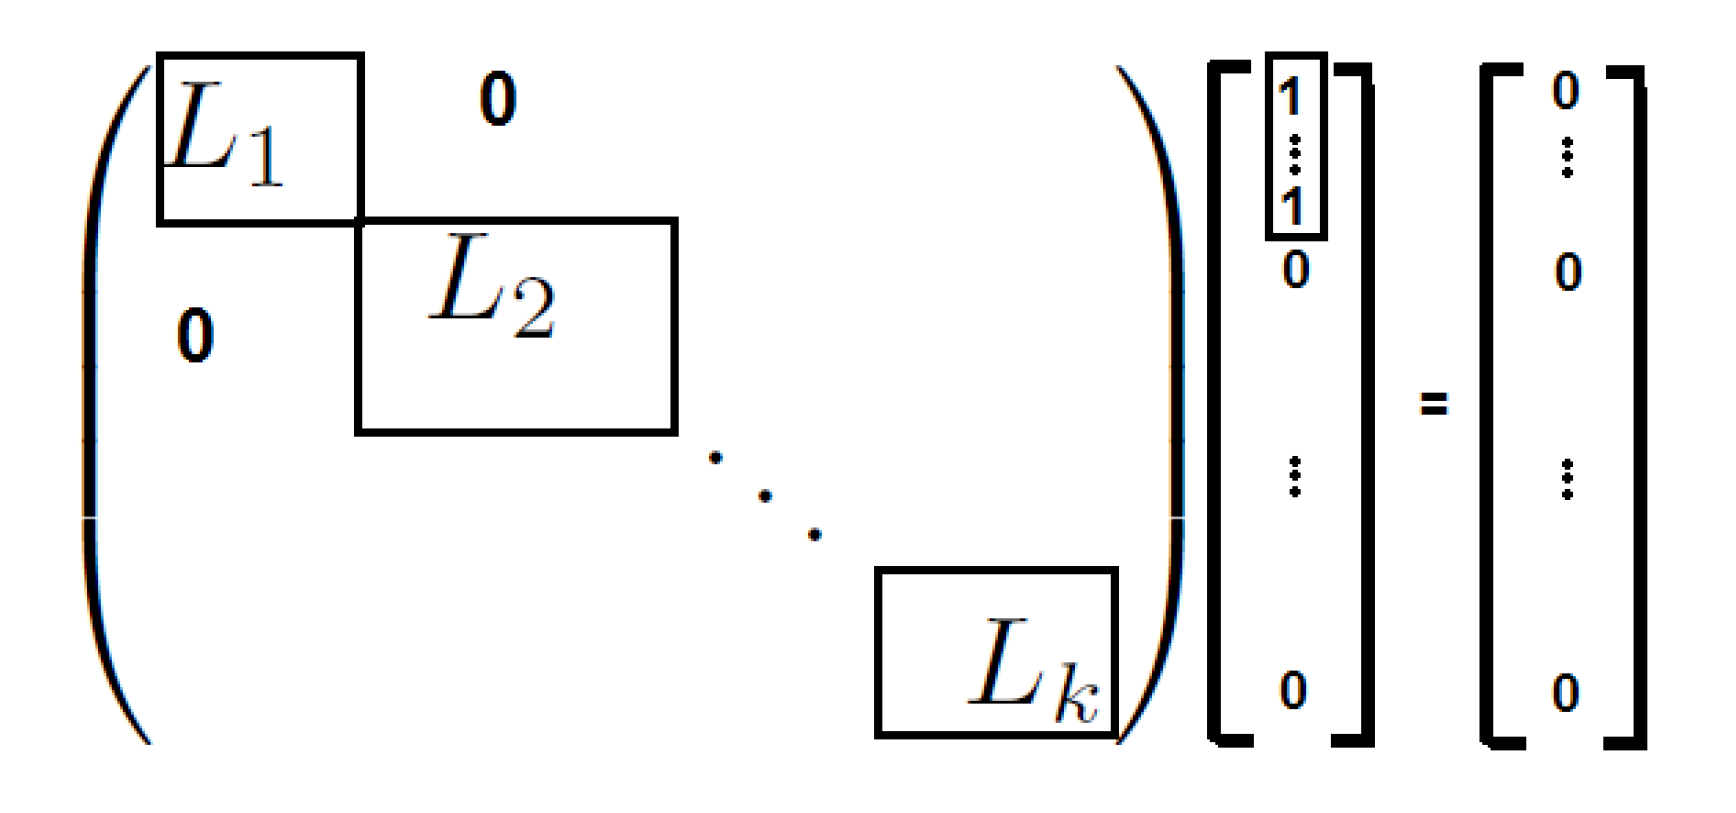
\includegraphics[scale=0.3]{Images/Laplacian.png}
	\caption{بردار ویژه متناظر با مقدار ویژه صفر در ماتریس لاپلاسین گراف دارای $k$ مولفه همبند} \label{Fig Laplacian}
\end{figure}

	\item گراف همبند که دارای یک مولفه همبندی است، تنها یک مقدار ویژه برابر با صفر دارد که بردار متناظر با آن برداری است که تمام المان‌های آن 1 باشد.

\end{enumerate}

حال که خواص ماتریس لاپلاسین بررسی شد، در قسمت بعد پایداری رابطه \ref{eq x. = -Lx} اثبات می‌گردد.

\newpage
\subsection{پایداری کنترل اجماع}
در کنترل اجماع، موقعیت عامل رهبر، $x_m$، به سیستم وارد می‌شود و کنترل اجماع تاثیری بر روی آن ندارد و $_l\dot{x}$ از طریق الگوریتم مسیریابی تعیین می‌گردد. لذا در رابطه \ref{eq x. = -Lx} سطر اول $L$ برابر صفر می‌گردد. به عنوان مثال در این پروژه، $L$ جدید، طبق رابطه \ref{eq L example} برابر است با:
\begin{equation}
L = 
\begin{bmatrix}
0~~~~~~0~~~~~~~0~~~~~~0 \\
-1~~~~~~3~~~-1~~~-1 \\
-1~~~-1~~~~~~3~~~-1 \\
-1~~~-1~~~-1~~~~~~3
\end{bmatrix}
\end{equation}

اگر $x$ برای مسئله یک رهبر و $n$ عامل دیگر به صورت زیر تعریف گردد:
\begin{equation}
x = 
\begin{bmatrix}
x_m \\
x_1 \\
x_2 \\
\vdots \\
x_n
\end{bmatrix}
\end{equation}

می‌توان $x_m$ را به صورت ورودی سیستم در نظر گرفت و سیستم را به شکل زیر بازنویسی کرد:
\begin{equation}\label{eq platoon system}
	\dot{x} = Ax + Bu, u = x_m
\end{equation}

که در آن $A$ و $B$ به شکل زیر از روی درایه‌های ماتریس $L$ به دست می‌آیند:
\begin{equation}\label{eq platoon AB}
A = 
\begin{bmatrix}
l_{22}~l_{23}~\cdots~l_{2n} \\
l_{32}~l_{33}~\cdots~l_{3n} \\
~~~~~~~~~\vdots~~~~~~~~~\\
l_{n2}~l_{n3}~\cdots~l_{nn} 
\end{bmatrix}
, B = 
\begin{bmatrix}
l_{21}\\
l_{31}\\
\vdots\\
l_{n1} 
\end{bmatrix}
\end{equation}

چون ماتریس اولیه لاپلاسین بوده پس اگر مقادیر هر سطر $B$ را از درایه قطر اصلی ماتریس $A$ که همان درایه قطر اصلی ماتریس لاپلاسین اولیه است کم کنیم به یک ماتریس لاپلاسین می‌رسیم. از اینجا به بعد منظور از ماتریس $L$ ماتریسی است که در تعریف زیر آمده است.
\begin{equation}\label{eq ABL relation}
	A + diag(B) = -L,~ diag(B) = 
	\begin{bmatrix}
	B_1~~0~~\cdots~~~~0 \\
	0~~~B_2~\cdots~~~0 \\
	~~~\vdots~~~\\
	~0~~~~0~~\cdots~~B_n
	\end{bmatrix}
\end{equation}

همچنین در ادامه منظور از ماتریس $\mathbbm{1}$ ماتریسی است که تمام درایه‌های آن 1 باشند.

ماتریس خطا، $e$، به صورت زیر تعریف می‌شود:
\begin{equation}\label{eq e definition}
	e = x - \mathbbm{1}x_m
\end{equation}

به کمک روابط \ref{eq platoon system} و \ref{eq ABL relation} داریم:
\begin{equation}\label{eq stability proof temp}
\dot{x} = Ax + Bx_m = -Lx - diag(B) + Bx_m
\end{equation}

با ادغام روابط \ref{eq stability proof temp} و \ref{eq e definition} می‌توان نوشت:
\begin{equation}
\dot{x} = -Le + L\mathbbm{1}x_m - diag(B)e
\end{equation}

با توجه به رابطه \ref{eq L1 = 0}، رابطه بالا به صورت زیر تبدیل می‌گردد:
\begin{equation}\label{eq x. = -Le -Be}
\dot{x} = -Le - diag(B)e
\end{equation}

که با کمک از رابطه \ref{eq ABL relation} می‌توان به رابطه زیر رسید:
\begin{equation}
	\dot{x} = Ae
\end{equation}

در نهایت چون بر متغیر $\dot{x}_m$ کنترلی نداریم و قرار است مطابق الگوریتم مسیریابی مقدار گیرد، آن را در هر فریم موقعیت عامل رهبر را ثابت می‌گیریم و در نتیجه می‌توان از مشتق آن صرف نظر کرد. با این فرض، سیستم دارای اندکی تاخیر می‌شود ولی در ادامه با اثبات پایدار مجانبی فراگیر\LTRfootnote{Globally asymptotically stable} بودن سیستم، مطمئن خواهیم بود که هنگام توقف خطا صفر خواهد بود. در نتیجه فرض بالا داریم:
\begin{equation}\label{eq x. = e.}
	\dot{x} = \dot{e}
\end{equation}

با استفاده از دو رابطه \ref{eq x. = -Le -Be} و \ref{eq x. = e.} نتیجه می‌شود:
\begin{equation}\label{eq dot e}
	\dot{e} = -Le -diag(B)e
\end{equation}

حال تابع کاندید لیاپانوف\LTRfootnote{Lyapunov candidate function}، $V(e)$، به صورت زیر تعریف می‌گردد، 
\begin{equation}\label{eq V definition}
V(e) = \frac{1}{2}e^Te > 0
\end{equation}

مشتق آن برابر است با:
\begin{equation}\label{eq V. = ee.}
\dot{V}(e) = e^T\dot{e}
\end{equation}

با جایگذاری رابطه \ref{eq dot e} در \ref{eq V. = ee.} خواهیم داشت:
\begin{equation}\label{eq V.}
\dot{V}(e) = -e^TLe - e^Tdiag(B)e
\end{equation}

حال به بررسی رابطه \ref{eq V.} می‌پردازیم. اولا طبق خواص مطرح شده در قسمت \ref{sec laplacian properties} و ماتریس مثبت معین بودن هر ماتریس لاپلاسینی داریم:
$\forall x,L~~x^TLx \ge 0$
 
در نتیجه در رابطه \ref{eq V.} داریم:
\begin{equation}\label{eq -ele<0}
	-e^TLe \le 0
\end{equation}

از طرفی با توجه به تعریف درایه‌های $B$ در رابطه \ref{eq platoon AB} که هیچ‌ یک درایه‌های قطر اصلی ماتریس لاپلاسین نیستند، درایه‌های $B$ می‌توانند یا صفر و یا یک باشند ولی حداقل یک درایه یک داریم، زیرا گراف همبند است و باید از عامل رهبر ارتباطی با بقیه موجود باشد. لذا اگر اندیس عامل‌هایی را که با عامل رهبر در ارتباط اند در مجموعه $N$ نگهداری کنیم داریم:
\begin{equation}\label{eq -ebe<0}
	-e^Tdiag(B)e = -\sum_{\forall j \in N}^{}e^2_j \le 0
\end{equation}

در نتیجه با توجه به روابط \ref{eq V.}، \ref{eq -ele<0} و \ref{eq -ebe<0} داریم:
\begin{equation}\label{eq V<0}
	\dot{V}(e) \le 0
\end{equation}

حال اثبات می‌کنیم که سیستم بالا پایدار مجانبی فراگیر است.

\begin{theorem}\label{th g.a.stable}
سیستم پایدار مجانبی است، اگر تنها یک نقطه تعادل پایدار داشته و تابع اسکالر $V(e)$ وجود داشته باشد که شرایط زیر را برآورده سازد:
\begin{enumerate}
	\item $V(e)$ در تمامی فضای حالت پیوسته و مشتق‌های جزئی پیوسته دارد.
	\item $V(e) > 0$ برای $x \ne 0$
	\item $V(0) = 0$
	\item $V(e) \to \infty$ به ازای $\|x\| \to \infty$
	\item $\dot{V}(e) \le 0$
و پاسخ غیر صفر 
$\dot{V}(e) = 0$
پاسخی از معادله دیفرانسیل سیستم نیست.
\end{enumerate}
\end{theorem}

شرایط 1 تا 4 توسط رابطه \ref{eq V definition} به دست می‌آیند. قسمت اول شرط 5، در رابطه \ref{eq V<0}
به دست آمده است. در ادامه قضیه \ref{th V. = 0} را اثبات می‌کنیم.

\begin{theorem}\label{th V. = 0}
اگر $e \ne 0$ وجود داشته باشد به طوری که $\dot{V} = 0$ باشد، آنگاه پاسخی از معادله دیفرانسیل سیستم نیست.

\end{theorem}

با برهان خلف قضیه را اثبات می‌کنیم. فرض خلف: فرض می‌کنیم $e_j$ وجود دارد به ظوری که 
$\dot{V}(e) = 0$.
تا به الان از فرض مهمی که در اثبات پایداری استفاده نشده است، همبند بودن گراف است. گفته شد چون گراف باید همبند باشد، پس از عامل رهبر به حداقل یکی از عامل‌ها باید ارتباط مستقیم وجود داشته باشد. در نتیجه حداقل یکی از درایه‌های بردار $B$ برابر 1 است. یکی از آن درایه‌ها را انتخاب می‌کنیم 
$B_i = 0$.
با توجه به رابطه \ref{eq V.} اگر $e_i \ne 0$ باشد، آنگاه عبارت 
$-e^TBe < 0$
خواهد بود که به همراه \ref{eq -ele<0} نتیجه می‌دهد 
$\dot{V}(e) < 0$ 
و به تناقض می‌رسیم. در نتیجه 
$e_n = 0$
باید باشد.

حال چون 
$e \ne 0$
در نتیجه درایه‌ای همانند   
$e_j \ne 0$ 
وجود دارد. حال از روی اینکه 
$\dot{e} = 0$ 
یا در حالت کلی 
\begin{equation}
\forall i = 1,2,...,n ~~ \dot{e}_i = 0
\end{equation}
باشد به تناقض خواهیم رسید. چون گراف همبند است پس هیچ راسی دارای درجه صفر نیست، لذا تمام داریه‌های قطر اصلی ماتریس $A$ غیر صفر هستند. اگر فقط درایه 
$e_j \ne 0$
داشته باشیم، در نتیجه چون داریه قطر اصلی متناظر با سطر $j$ مخالف صفر است، 
$\dot{e}_j \ne 0$
می‌شود. پس اگر $W$ مجموعه‌ی اندیس تمامی عامل‌های غیر لیدر باشد آنگاه $J$ را کوچک‌ترین مجموعه‌ای در نظر می‌گیریم به طوری که  
$J \subset W $
 از اندیس‌ها باشد به طوری که 
\begin{equation}
	\forall j \in J~~ e_j \ne 0
\end{equation}

و نتیجه دهد 
$\dot{e} = 0$.

دلیل اینکه امکان ندارد 
$J = W$
باشد این است که باید
$e_y = 0$
باشد.

حال دو حالت داریم: یا تمامی $e_{ji}$ ها با هم برابرند یا حداقل یک جفت وجود دارند که با هم ارتباط مستقیم دارند و در آن یکی از دیگری بزرگتر است.

اگر تمامی $e_{ji}$ با هم برابر و دارای مقدار $c$ باشند، به معنی آن است که اگر یک بردار $z$ تشکیل دهیم که متناظر با سطر $ji$ مقدار $c$ و در بقیه سطرها مقدار صفر بگیرد
$e = z$
، طبق رابطه \ref{eq dot e} داریم:
\begin{equation}\label{eq e. = -Lz - Bz}
	\dot{e} = -Lz~~-diag(B)z = 0
\end{equation}

و چون سطرهایی که $B_i = 1$ است، 
$z_i = 0$
است، خواهیم داشت:
\begin{equation}\label{eq Bz = 0}
	diag(B)z = 0
\end{equation}

با ادغام روابط \ref{eq e. = -Lz - Bz} و \ref{eq Bz = 0} داریم:
\begin{equation}
	Lz = 0
\end{equation}

که نتیجه می‌دهد $z$ بردار ویژه $L$ است و چون 
$z \ne \mathbbm{1}$
پس $L$ حداقل 2 مقدار ویژه مخالف صفر دارد که این با همبند بودن گراف اجماع در تناقض است. در نتیجه برای اینکه حالت بالا پیش نیاید جفت 
$|e_{j2}| > |e_{j1}|$
در مجموعه $J$ وجود دارند که دارای ارتباط مستقیم هستند.

نکته قابل توجه این است که در سطرهای عناصر $J$، درایه قطر اصلی برابر منفی مجموع درایه‌های دیگر است. در نتیجه اگر قدرمطلق درایه قطر اصلی در سطر $i \in J$ برابر $k_i$ باشد داریم:
\begin{equation}\label{eq sum in row}
	k_i e_{i} = \sum_{t \in T_i}^{}e_{t},~~ |T_i| = k_i
\end{equation}

که در آن $T_i$ مجموعه $t$هایی در سطر $i$ است که 
$a_{it} = 1$
باشد.

حال اگر سطر $j2$ را در نظر بگیریم، با توجه به رابطه \ref{eq sum in row} و 
$j1 \in T_{j2}$
داریم:
\begin{equation}\label{eq e > e}
\exists j3 \in T_{j2}~~|e_{j3}| > |e_{j2}|
\end{equation}

رابطه \ref{eq e > e}، مرنبا تکرار می‌شود و به $e_{j4}$ و بقیه $e_{ji}$ ها می‌رسیم. در نهایت چون یک رابطه خوش‌ترتیبی بیان گشته و مجموعه $W$ و در نتیجه آن $J$ متناهی است، عضوی همانند $e_jx$ وجود دارد که عضوی بزرگتر از اندازه آن در $J$ و چون بقیه‌ $e_i$ ها نیز برابر صفر هستند، عضوی بزرگتر از اندازه آن در بین کل $e_i$ها وجود ندارد. همچنین چون 
\begin{equation}\label{eq ejk-1 < ejx}
\exists j(x-1) \in T_{jx}~~s.t.~~|e_{j(x-1)}| < |e_{j(x)}|
\end{equation}

طبق رابطه \ref{eq sum in row} در سطر $jx$ داریم:
\begin{equation}\label{eq sum in row jx}
k_{jx} e_{jx} = e_{j(x-1)} + \sum_{t \ne j(x-1) \in T_{jx}}^{}e_{t},~~ |T_{jx}| = k_{jx}
\end{equation}

اگر از دو طرف رابطه \ref{eq sum in row jx}، قدرمطلق بگیریم داریم:
\begin{equation}\label{eq sum || in row jx}
k_{jx} |e_{jx}| = |e_{j(x-1)}| + \sum_{t \ne j(x-1) \in T_{jx}}^{}|e_{t}|,~~ |T_{jx}| = k_{jx}
\end{equation}

که با در نظر گرفتن روابط \ref{eq ejk-1 < ejx} و \ref{eq sum || in row jx}، نتیجه می‌شود که 
\begin{equation}
\exists t \in T_{jx}~~s.t.~~|e_t|>|e_jx|
\end{equation}

و این عبارت تناقض است.

در نتیجه تمامی شرایطی که در نظر گرفتیم، به تناقض رسید، پس فرض خلف باطل و حکم که قضیه \ref{th V. = 0} است، ثابت می‌گردد.

در نتیجه تمامی شرایط قضیه \ref{th g.a.stable} برقرار می‌گیرد و سیستم پایدار مجانبی فراگیر خواهد بودو خطا به صفر خواهد رسید.

\subsection{روش شکل‌دهی}
با رابطه \ref{eq x. = -Lx} به این رسیدیم که اگر یکی از عامل‌ها را رهبر در نظر بگیریم، بقیه آن را دنبال خواهند کرد. حال با یک حقه، ماتریس شکل‌دهی\LTRfootnote{formation} را تعریف و اعمال می‌کنیم. نسبت اختلاف موقعیت هر ربات را در $F$ که ماتریس شکل‌دهی است، قرار می‌دهیم و با رابطه \ref{eq x. = -L(x-f)}، کاری می‌کنیم که موقعیت واقعی عامل $i$ با اختلاف $F_i$ دیده شود و در نتیجه وقتی عامل میخواهد به موقعیت مطلوب $x_{di}$ برود در واقعیت به موقعیت $x_{di} + F_i$ خواهد رسید که همان هدف ما از شکل‌دهی است.
\begin{equation}\label{eq x. = -L(x-f)}
	\dot{x} = -L(x-F)
\end{equation} 

همچنین چون در دو بعد $x-y$ مشغول به کار هستیم، بردار $x$ را به ماتریس با دو ستون تغییر دادیم به طوری که یک ستون مربوط به فاصله در محور $x$ و یک ستون مربوط به فاصله در محور $y$ باشد. و در نتیجه ماتریس شکل‌دهی نیز دارای 2 ستون است.
\begin{equation}\label{eq X = [x y]}
	X = 
	\begin{bmatrix}
	x_1~~ y_1 \\
	x_2~~ y_2 \\
	\vdots \\
	x_n ~~y_n
	\end{bmatrix}
\end{equation}

\section{شبیه‌سازی و نتایج}






\chapter{مسیریابی}\label{ch path planning}

\section{مقدمه}

به طراحی مسیری امن به طوری که بدون برخورد با موانع از قرارگیری اولیه، که شامل مکان و زاویه‌ها، به طور کلی تمام پارامترهای توصیف یک جسم در فضای محیط، به قرارگیری نهایی است، مسیریابی\LTRfootnote{path planning} می‌گویند. در این پروژه می‌توان مکان ربات‌ها و موانع را به عنوان حالت\LTRfootnote{state} در نظر گرفت. با توجه به اینکه دید از بالا فرض شده است به نحوی که از تمام مکان‌ها اطلاع داشته باشیم، در نتیجه نسبت به تمام موانع اطلاع دقیقی داریم. پس می‌توان گفت در هر حالت نسبت به محیط و داده‌ها به طور کامل مطلع\LTRfootnote{informed} هستیم. در این فصل ابتدا روش میدان پتانسیل و سپس الگوریتم‌های مسیریابی مبتنی بر روش‌های ابتکاری\LTRfootnote{heuristic} که لازمه آن‌ها مطلع بودن از محیط است، پیاده‌سازی و بررسی گشته‌اند.

\section{میدان پتانسیل}
در این روش یک میدان دافعه و جاذبه ایجاد می‌کنیم و ربات در راستای میدان حرکت خواهد کرد. ایده اصلی این است که نقطه‌ی هدف را به صورت جاذبه و نقاطی که مانع هستند را به صورت دافعه در نظر بگیریم (همانند میدان الکتریکی و بارهای همنام و ناهمنام). در نتیجه، ربات به سمت نقطه هدف کشیده خواهد شد.

\subsection{روابط میدان پتانسیل}
رابطه میدان پتانسیل جذبی برای \verb|i|امین ربات از طرف بار ناهمنام یا به عبارتی موقعیت هدف که یک چاه پتانسیل سهمی‌گون ایجاد می‌کند، به شرح زیر است:
\begin{equation}\label{eq Uatt}
U_{att,i} = 
\begin{cases*}
\frac{1}{2}\zeta_i\|o_i(q) - o_i(q_f)\|^2 & \verb|if| $\|o_i(q) - o_i(q_f)\| \le d$ \\
d\zeta_i\|o_i(q) - o_i(q_f)\|-\frac{1}{2}\zeta_id^2 & \verb|otherwise|
\end{cases*}
\end{equation}

که در آن منظور از $o_i(q_i)$ موقعیت ربات \verb|i|ام، $o_i(q_f)$ موقعیت مطلوب ربات، $\zeta_i$ ضریبی است که بعدا در روش گرادیان نزولی به ضریب آن تبدیل می‌گردد و $d$ فاصله گذر از چاه مخروطی را تعیین می‌کند. علت تعریف میدان به صورت فوض این است که در مرز $d$ هر دو برابر باشند و ناپیوستگی نداشته باشیم.

می‌دانیم $F_{att,i} = -\nabla U_{att,i}$ در نتیجه به توجه به رابطه \ref{eq Uatt} خواهیم داشت:
\begin{equation}
F_{att,i} = 
\begin{cases*}
-\zeta_i(o_i(q) - o_i(q_f)) & \verb|if| $\|o_i(q) - o_i(q_f)\| \le d$ \\
-d\zeta_i \frac{(o_i(q) - o_i(q_f))}{\|o_i(q) - o_i(q_f)\|} & \verb|otherwise|
\end{cases*}
\end{equation}

برای جلوگیری از برخورد با موانع میدان پتانسیل دفعی به صورت زیر تعریف کرد. این میدان ربات را از موانع دور کرده و اجازه برخورد ربات با مانع را نمی‌دهد. همچنین وقتی ربات از مانع دور است نباید نیرویی از طرف مانع به ربات اعمال گردد. به همین دلیل تابع پتانسیل باید طوری تعریف شود که به هنگام رسیدن ربات به مانع مقدارش بی‌نهایت و در یک فاصله مشخص از مرز مانع صفر گردد. این تابع پتانسیل برای ربات \verb|i| و مانع \verb|j| به شکل زیر تعریف می‌گردد:
\begin{equation}\label{eq Urep}
U_{att,ij} = 
\begin{cases*}
\frac{1}{2}\eta_{ij}(\frac{1}{\rho_j(o_i(q))} - \frac{1}{\rho_{0j}})^2 & \verb|if| $\rho_j(o_i(q)) \le \rho_{0j}$\\
~~~~~~~~~~~0 & \verb|otherwise|
\end{cases*}
\end{equation}

که در آن $\rho_j(o_i(q))$ و $\rho_{0j}$ به ترتیب برابر یا کوتاه‌ترین فاصله بین $i$امین ربات و $j$امین مانع، و فاصله تاثیر $j$امین مانع هستند. با رابطه $F_{rep,ij} = -\nabla U_{rep,ij}$ و \ref{eq Urep} خواهیم داشت:
\begin{equation}\label{eq Frep}
F_{att,ij} = 
\begin{cases*}
\eta_{ij}(\frac{1}{\rho_j(o_i(q))} - \frac{1}{\rho_{0j}}) \frac{1}{\rho^2_j(o_i(q))} \frac{o_i(q)-o_j(q)}{\|o_i(q)-o_j(q)\|} & \verb|if| $\rho_j(o_i(q)) \le \rho_{0j}$\\
~~~~~~~~~~~0 & \verb|otherwise|
\end{cases*}
\end{equation}

در نهایت نیروی کل اعمالی به ربات به صورت زیر خواهد بود:
\begin{equation}\label{eq Ftot}
	F_{tot,i} = F_{att,i} + \sum_{j \in obstacles}^{}F_{rep,ij}
\end{equation}

در ادامه نحوه استفاده از نیرو توضیح داده خواهد شد.

\subsection{کنترل مسیر ربات با میدان پتانسیل}
برای این هدف نیروی اعمالی به ربات که در قسمت قبل محاسبه شد را به عنوان سرعت مطلوب به کنترل‌کننده تک ربات اعمال کردیم تا ربات به سرعت، مسیر خود را تغییر و به جهت مناسب حرکت نماید. مسیر پیموده شده توسط ربات با میدان پتانسیل در شکل \ref{Fig potential-field-1robot-pos} آمده است.
\begin{figure}[!h]
	\centering
	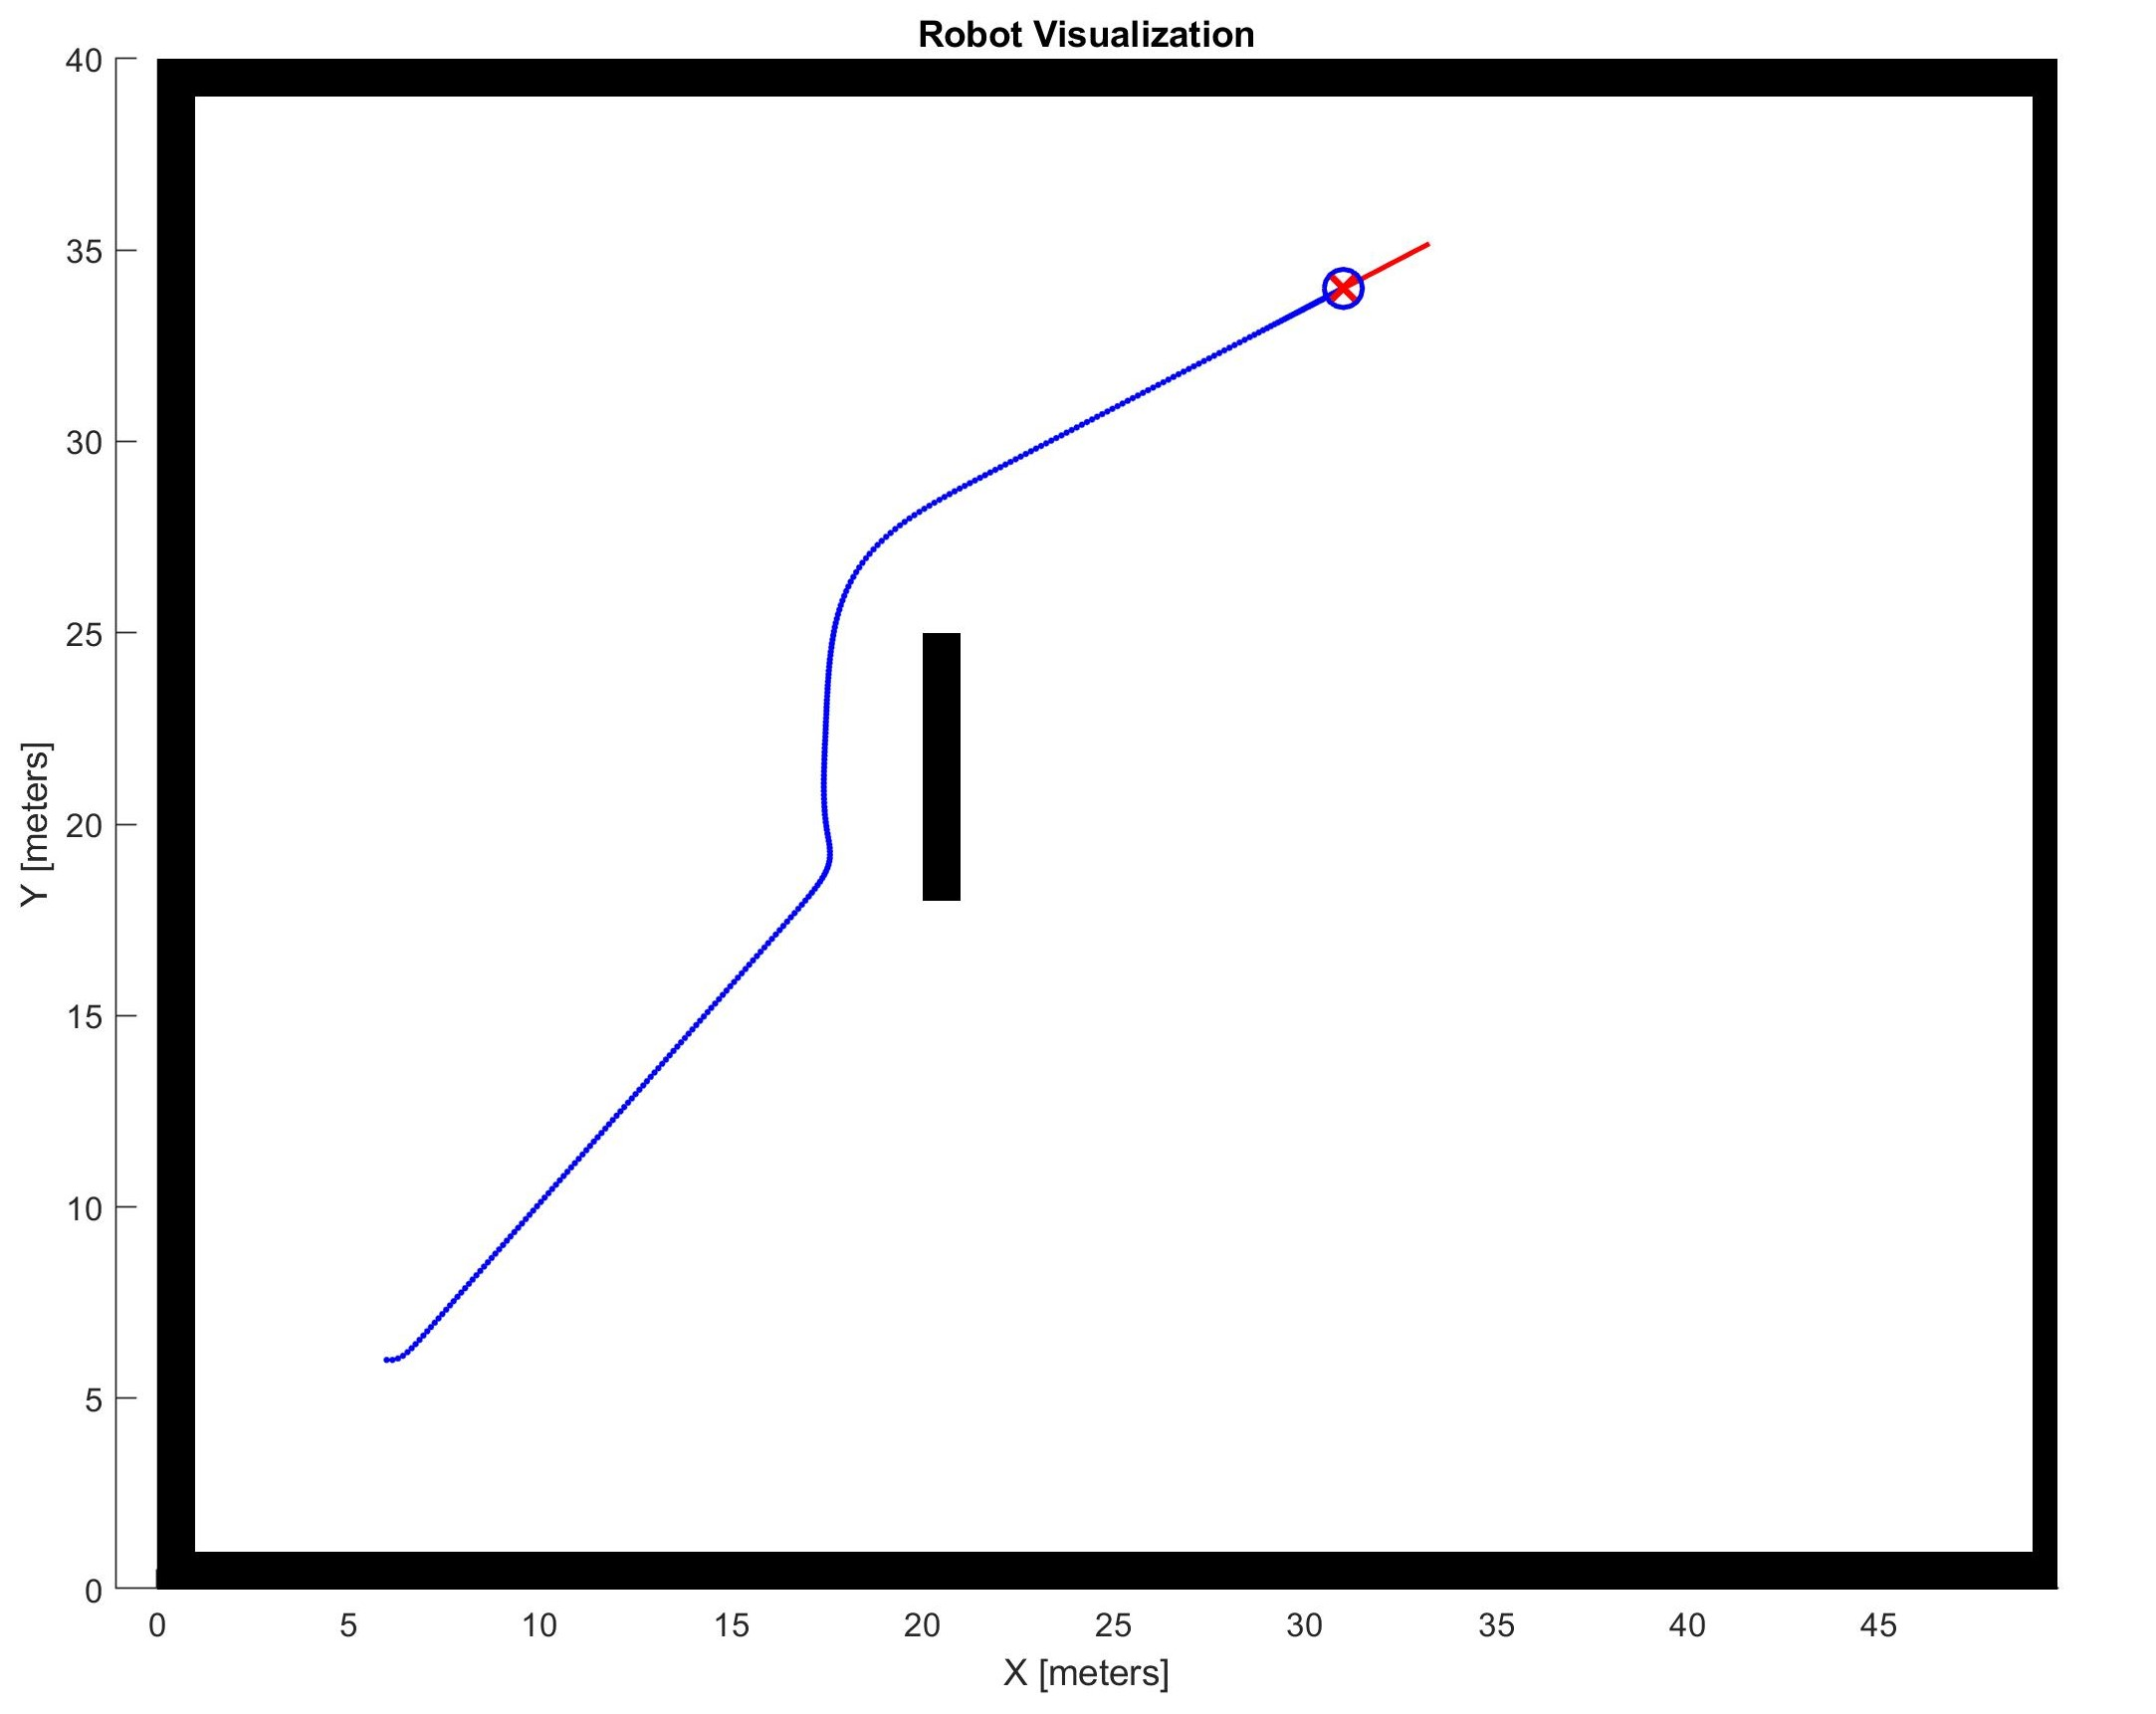
\includegraphics[scale=0.28]{Images/potential-field-1robot-pos.jpg}
	\caption{مسیر پیموده شده توسط ربات با میدان پتانسیل}\label{Fig potential-field-1robot-pos}
\end{figure}

یکی از مشکلات اصلی میدان پتانسیل این است که لزوما جواب ندارد و امکان دارد ربات در کمینه\LTRfootnote{minimum} محلی متوقف شود. به عنوان مثال در شکل \ref{Fig potential-field-1robot-stuck}، ربات در کمینه محلی گیر کرده و به نقطه هدف نرسیده است.
\begin{figure}[!h]
	\centering
	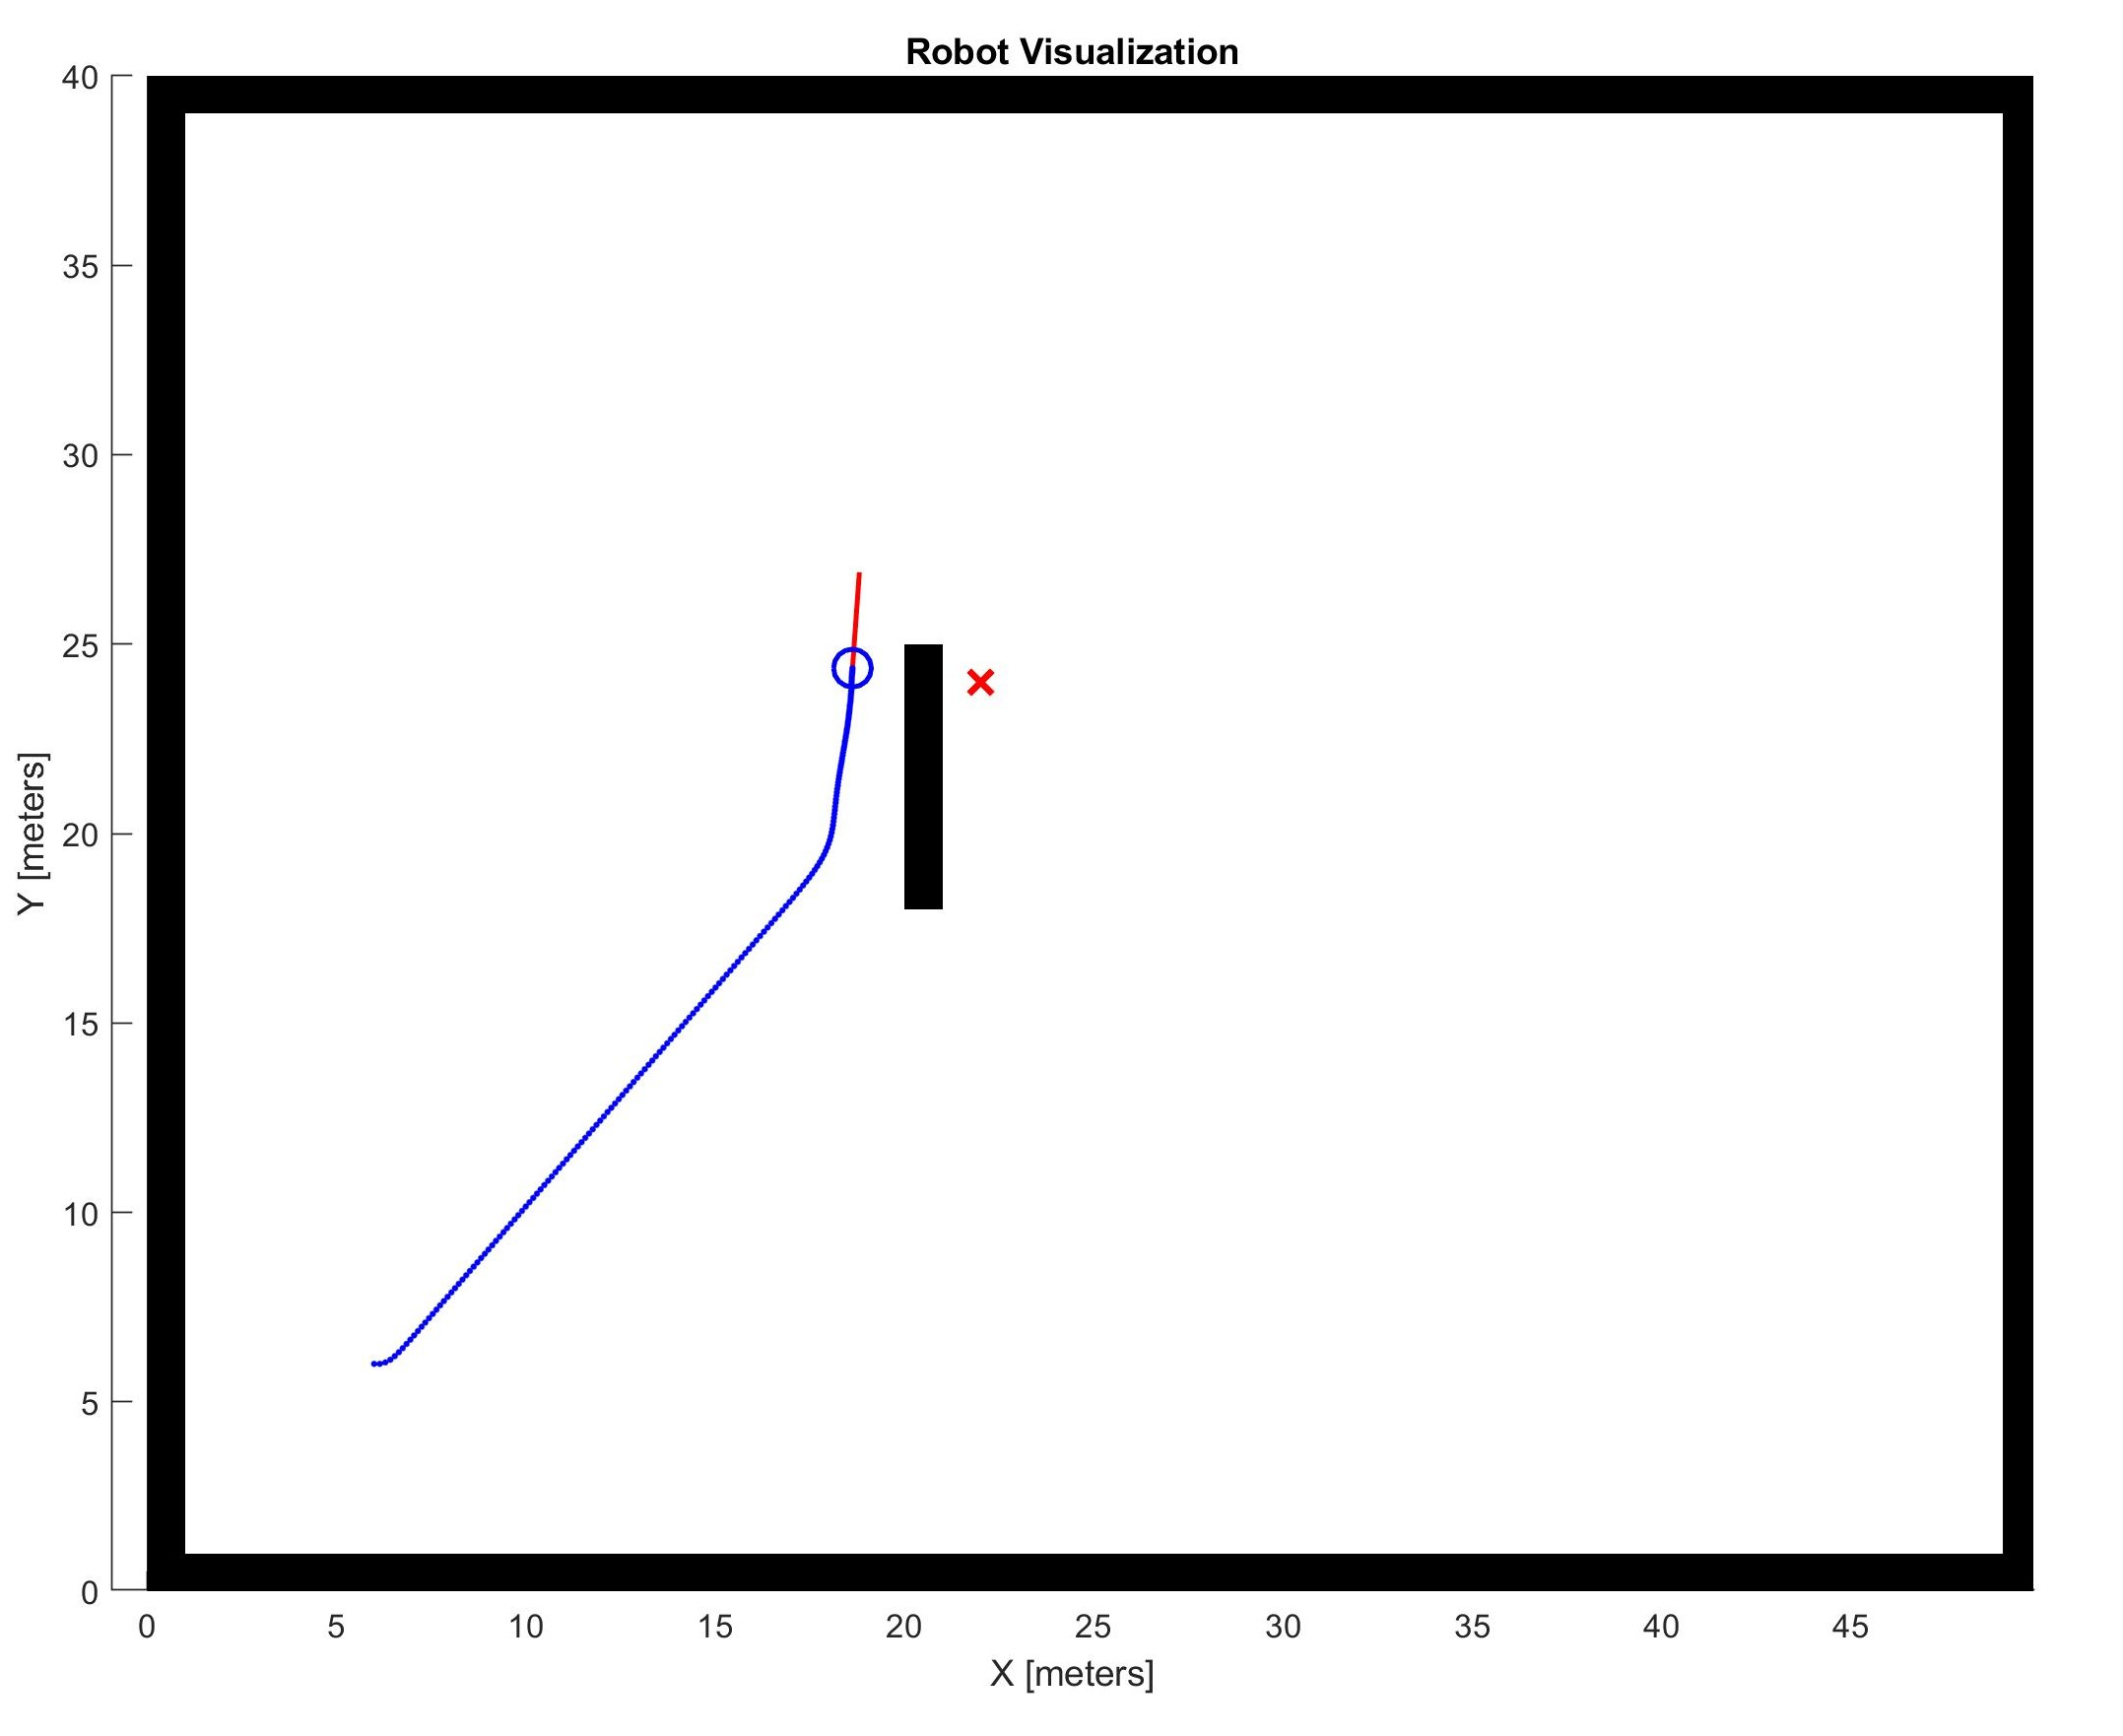
\includegraphics[scale=0.28]{Images/potential-field-1robot-stuck.jpg}
	\caption{گیر کردن ربات در کمینه محلی با میدان پتانسیل}\label{Fig potential-field-1robot-stuck}
\end{figure}

برای حل این مشکل معمولا نیرویی در جهت تصادفی به ربات وارد می‌گردد اما همچنان تضمینی برای خارج شدن از کمینه محلی\LTRfootnote{local minimum} وجود ندارد. لذا در ادامه به بررسی الگوریتم‌هایی می‌پردازیم که مطمئن هستیم حتما مسیری که به موقعیت مطلوب ختم می‌شود را می‌یابند.

\section{الگوریتم‌های ابتکاری}
همانطور که گفته شد، با توجه به شرایط مسئله و مطلع بودن در زمان طراحی مسیر، از الگوریتم‌های ابتکاری استفاده شده است. خصوصیت این الگوریتم‌ها در این است که با ابتکاری که به خرج داده می‌شود، مسئله اندکی ساده‌تر فرض شده و حل می‌گردد. مزیت این الگوریتم‌ها پیچیدگی زمانی کمتر آن‌ها نسبت به مسائلی هستند که مسئله مسیریابی را به طور کامل حل می‌نمایند. این امر در کاربرد رباتیک به دلیل اهمیت بلادرنگ\LTRfootnote{real time} بودن، دارای اهمیت بسیار زیادی می‌باشد. اما همانطور که گفته شد، چون مسئله به طور کامل حل نمی‌گردد، تضمینی برای رسیدن به پاسخ بهینه\LTRfootnote{optimal} وجود ندارد اما پاسخ به طور کلی معقول است، هر چند بهینه نباشد.

برای اعمال این الگوریتم‌ها نیاز به داشتن تعداد حالات محدود بود اما در بازه بین دو عدد متمایز در اعداد حقیقی، مجموعه حالات نامتناهی هستند. لذا از روش نمونه‌برداری\LTRfootnote{sampling based method} استفاده شد. در این پروژه، تمام نقاط با مختصات‌های اعداد صحیح را به عنوان حالت‌ها در نظر گرفتیم. همچنین مجموعه اقدامات\LTRfootnote{actions} به صورت حرکت به حالت‌های مجاور در راستاهای شمال، جنوب، شرق و غرب، و همچنین در راستاهای مورب شمال-غرب، شمال-شرق، جنوب-غرب و جنوب-شرق، تعریف شدند. مسیر خروجی نیز به صورت مجموعه‌ای مرتب از مختصات‌های مجاور که شروع آن مختصات اولیه و پایان آن مختصات نهایی می‌باشد، است. در این پروژه روش‌های ابتکاری \verb|BFS|\LTRfootnote{Breadth-first search}، \verb|search first best Greedy| و $A^*$ پیاده سازی شده‌اند که در ادامه به توضیح آن‌ها می‌پردازیم.

\subsection{الگوریتم $BFS$}
الگوریتم \verb|BFS| در اصل یکی از الگوریتم‌های سرچ معروف و پایه‌ای گراف می‌باشد. برای استفاده از این روش، گراف را به نحوی که هر راس نماینده فقط و فقط یک حالت مجاز، و همچنین هر اقدام نماینده فقط و فقط یک یال باشد ساختیم. همچنین وزن هر یال برابر با نرم-2\LTRfootnote{2-norm} بردار جابه‌جایی اقدام مربوطه، که همان فاصله در مختصات دکارتی است، در نظر گرفته شد. منظور از حالت مجاز، مختصاتی است که در آن مانع نباشد و در محدوده کاری قرار گیرد. حال الگوریتم \verb|BFS| بر روی گراف اعمال می‌شود. قابل ذکر است در صورتی که وزن تمام یال‌ها برابر باشند، اثبات می‌گردد که این الگوریتم به جواب بهین خواهد رسید.

نحوه کار این الگوریتم به این صورت است که با شروع از راس شروع، راس‌های مجاور بررسی می‌شوند و سپس وارد یک صف\LTRfootnote{queue} می‌گردند تا راس‌های مجاور آن‌ها بررسی گردد. صف در ابتدا تنها دارای راس شروع است. برای اینکه راس‌های تکراری وارد صف نگردند، از رنگ‌آمیزی راسی استفاده شد. به این صورت که در ابتدا همه راس‌ها سفید و تنها راس شروع، مشکی می‌باشد. سپس هر راسی که وارد صف می‌شود به رنگ مشکی در می‌آید. در نتیجه هنگام بررسی راس‌های مجاور ابتدا بررسی می‌گردد که چه رنگی دارد. زیرا اگر مشکی باشد یعنی قبلا بررسی شده و دیگر نیازی به بررسی نیست. اینکار تا زمانی که به راس هدف برسیم، ادامه خواهد یافت.

اگر گراف به صورت 
$G = (V, E)$
که در آن \verb|V| مجموعه راس‌ها و \verb|E| مجموعه یال‌ها می‌باشد، تعریف شود، الگوریتم اصلی \verb|BFS| در شکل \ref{Fig BFS Algorithm} به صورت شبه کد آمده است. منظور از نماد \verb|Q| در شبه کد، صف، منظور از \verb|d| فاصله و منظور از $\pi$ والد\LTRfootnote{parent} است. تفاوت در کد ارائه شده در این پروژه با این شبه کد، این است که احتیاجی به رنگ خاکستری نبود و رنگ خاکستری معادل رنگ مشکی در نظر گرفته شد. همچنین چون نقطه هدف داشتیم، در صورتی که به نقطه هدف می‌رسیدیم، حلقه خط 10 شکسته می‌شد و الگوریتم متوقف می‌گشت.
\begin{figure}[!h]
	\centering
	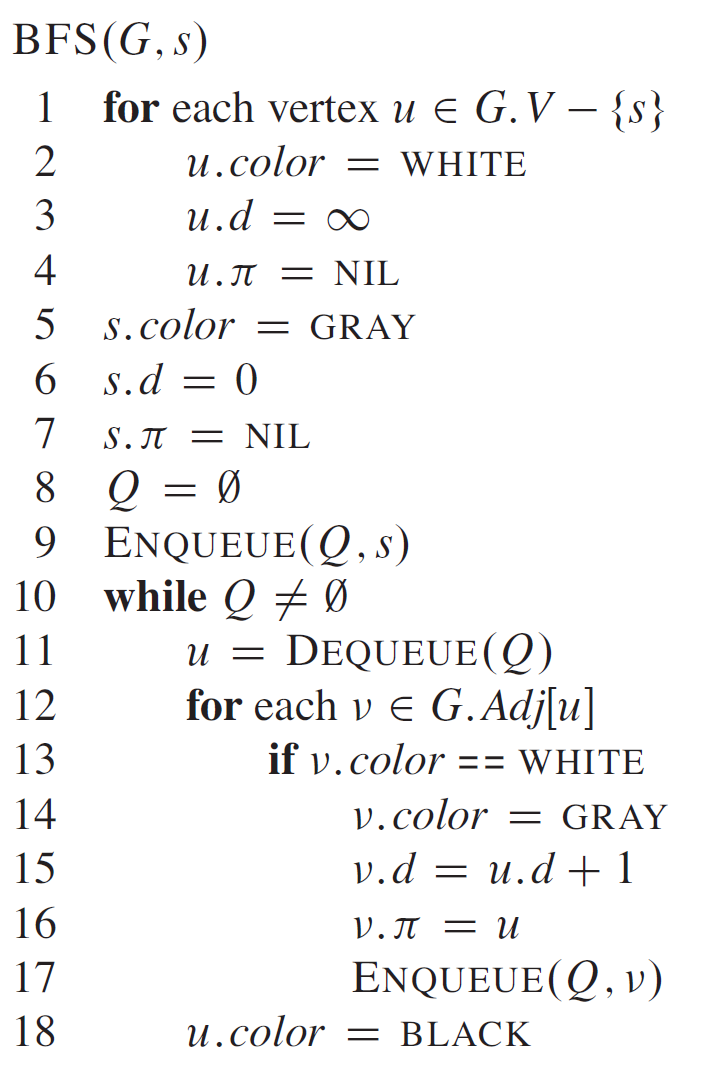
\includegraphics[scale=0.4]{Images/BFS-algorithm.png}
	\caption{شبه کد الگوریتم $BFS$}\label{Fig BFS Algorithm}
\end{figure}

 در شکل \ref{Fig BFS representation} نیز نحوه اعمال شدن الگوریتم \verb|BFS| بر روی یک گراف، نمایش داده شده است.
\begin{figure}[!h]
	\centering
	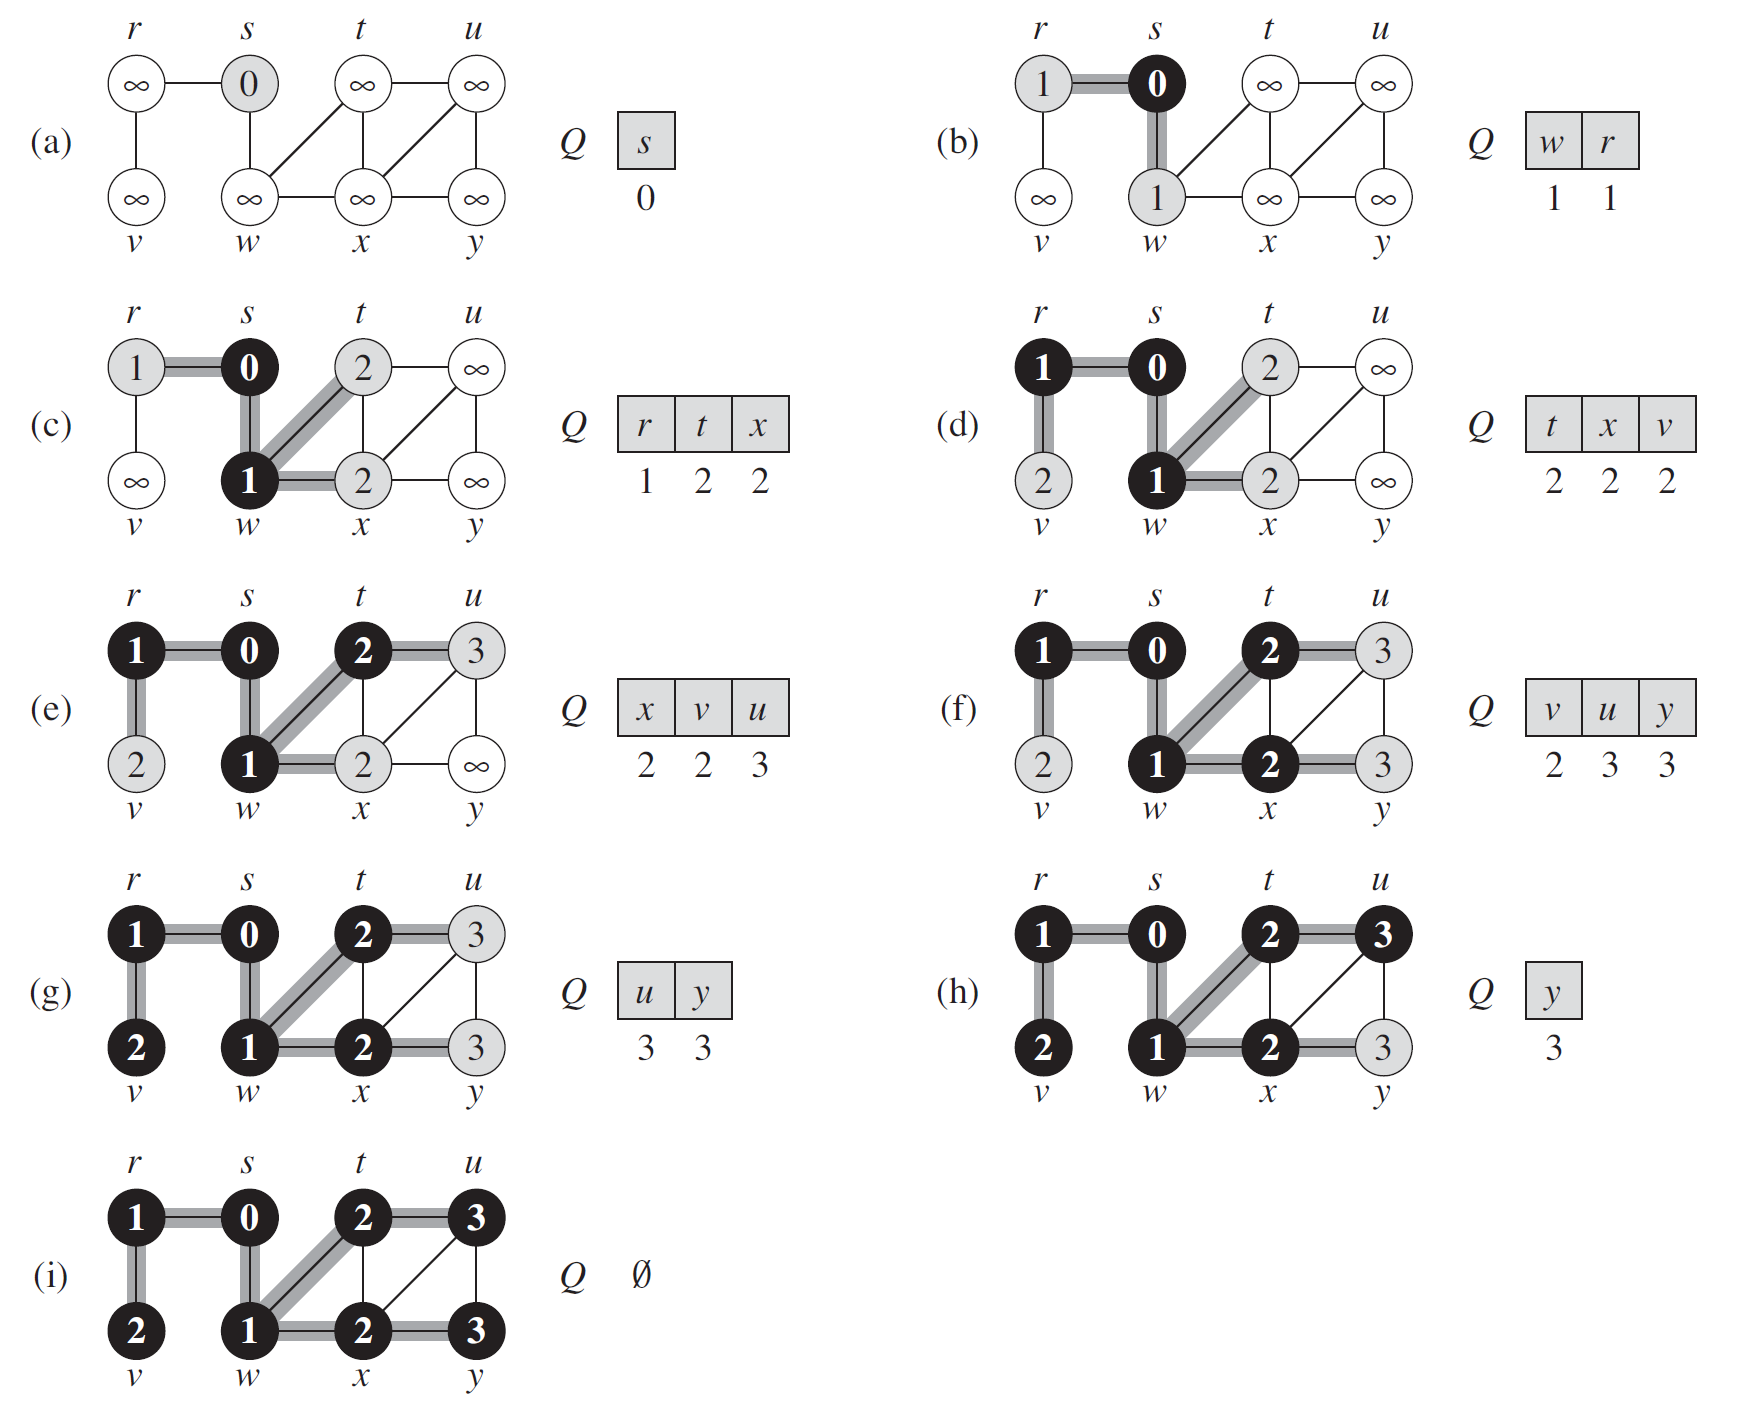
\includegraphics[scale=0.4]{Images/BFS-representation.png}
	\caption{نحوه اعمال شدن الگوریتم $BFS$}\label{Fig BFS representation}
\end{figure}


\newpage
\subsection{الگوریتم $search$ $best-first$ $Greedy$}
ابتکار این روش این است که سعی می‌کند به سمت راسی که کمترین فاصله تا راس هدف دارد، گسترش پیدا کند، به امید آنکه به کوتاه‌ترین مسیر دست یابد. چون کمترین فاصله تا راس هدف را نداریم، حد پایین آن‌ را تقریب می‌زنیم و برابر فاصله قرار می‌دهیم. برای تقریب حد پایین، چون مختصات دو راس را داریم، کافی است طول خط راستی که راس را به راس هدف می‌رساند به دست آورد. در این راستا تابع $h(n)$ برای مختصات راس، \verb|n|، تعریف می‌گردد. اگر مختصات راس هدف با $n^\prime$ نمایش داده شود، مقدار تابع $h(n)$ که طول خط راست از راس تا راس هدف است به صورت زیر تعریف می‌گردد:
\begin{equation}\label{eq heuristic h}
h(n) = \|n - n^\prime\|_2
\end{equation}

مشخصا این روش نیز لزوما به جواب بهین نمی‌رسد، زیرا اصلا می‌تواند بین راسی که انتخاب شده تا راس هدف مسیری نباشد و به بن بست برسیم و مجبور به برگشت باشیم. همچنین برای مثال نقض نیز می‌توان نتیجه این روش را در بخش \ref{sec heuristic result} بررسی کرد که جواب آن بهین نیست.

در هنگام جست‌وجو در هر گام، والد هر راس را در درخت مسیر، به روز می‌گردد و در انتها با کمک از همین والد‌ها و با شروع از راس هدف، تا راس شروع، به عقب برمی‌گردیم. برعکس این مسیر، مسیری خواهد بود که ربات باید بپیماید.

\subsection{الگوریتم $A^*$}
الگوریتم $A^*$ ادامه‌ای بر الگوریتم \verb|search first best Greedy| است که در آن علاوه بر تابع $h(n)$ که در رابطه \ref{eq heuristic h} تعریف شد، تابع $g(n)$ نیز تعریف می‌شود که مسافت واقعی بین نقطه شروع تا راس \verb|n| است. این فواصل با الگوریتم جست‌وجو مرتبا به روز می‌شود و در صورتی که مسیر کوتاه‌تری یافته شود نیز مقادیر آن به همراه مسیر واصله، به روز خواهند شد. همچنین برای یافتن کوتاه‌ترین مسیر نیز همانند الگوریتم \verb|search first best Greedy|، برای هر راس یک والد در نظر گرفته شده است و با پیدا کردن مسیری کوتاه‌تر، مقداری کمتر برای تابع $g(n)$ در راس \verb|n|، والد نیز به راس جدیدی که به آن مسیر دارد، تغییر می‌یابد.

تابعی که طبق آن، راسی که کمترین مقدار آن را داشته باشد جست‌وجو خواهد شد، $f(n)$ می‌نامیم، که به صورت زیر تعریف می‌گردد:
\begin{equation}%\label{eq heuristic f}
	f(n) = g(n) + h(n)
\end{equation}

در نهایت نیز هنگامی که به راس هدف برسیم، الگوریتم جست‌وجو متوقف می‌گردد و سپس به طور بازگشتی از راس هدف، بر روی والدها به عقب برمی‌گردیم تا با عکس کردن جهت حرکت، مسیر ربات تعیین شود. 


\subsection{نتایج و مقایسه الگوریتم‌های ابتکاری}\label{sec heuristic result}
در این قسمت ابتدا به بررسی مسیر یافته شده توسط الگوریتم‌ها پرداخته می‌شود و سپس الگوریتم‌ها از نظر زمانی و ابعاد نقشه، مورد بررسی قرار می‌گیرند.

نقشه مورد استفاده برای بررسی پاسخ‌ها در شکل \ref{Fig mapRooz} آمده است. نقاط مشکی رنگ، مکانی هستند که مانع وجود دارد.
\begin{figure}[!h]
	\centering
	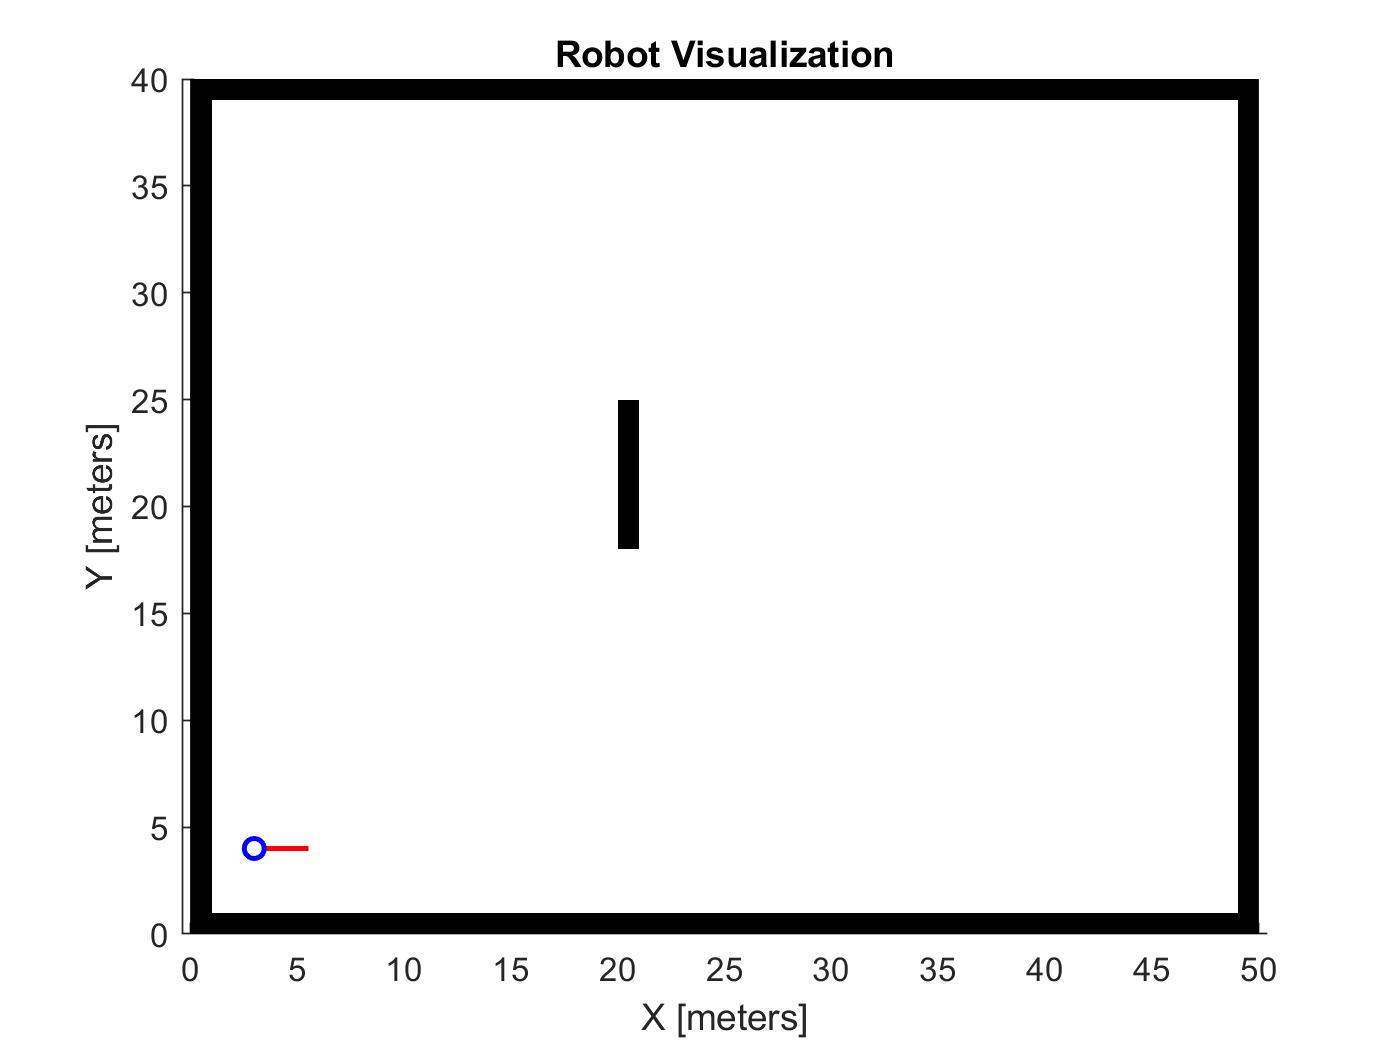
\includegraphics[scale=0.35]{Images/mapRooz.jpg}
	\caption{نقشه‌ای که الگوریتم‌ها به آن اعمال شده‌اند}\label{Fig mapRooz}
\end{figure}

حال برای هر سه الگوریتم، مسیری برای نقطه شروع $[6~~6]^T$ و هدف $[21~~24]^T$ خواسته شد. نتایج به شکل‌های \ref{Fig BFS path}، \ref{Fig Greedy path} و \ref{Fig A-star path} آمده است. نقاط ضربدر خورده قرمز، مسیر الگوریتم، و خط آبی مسیر پیموده شده توسط ربات هستند.
\begin{figure}[!h]
	\centering
	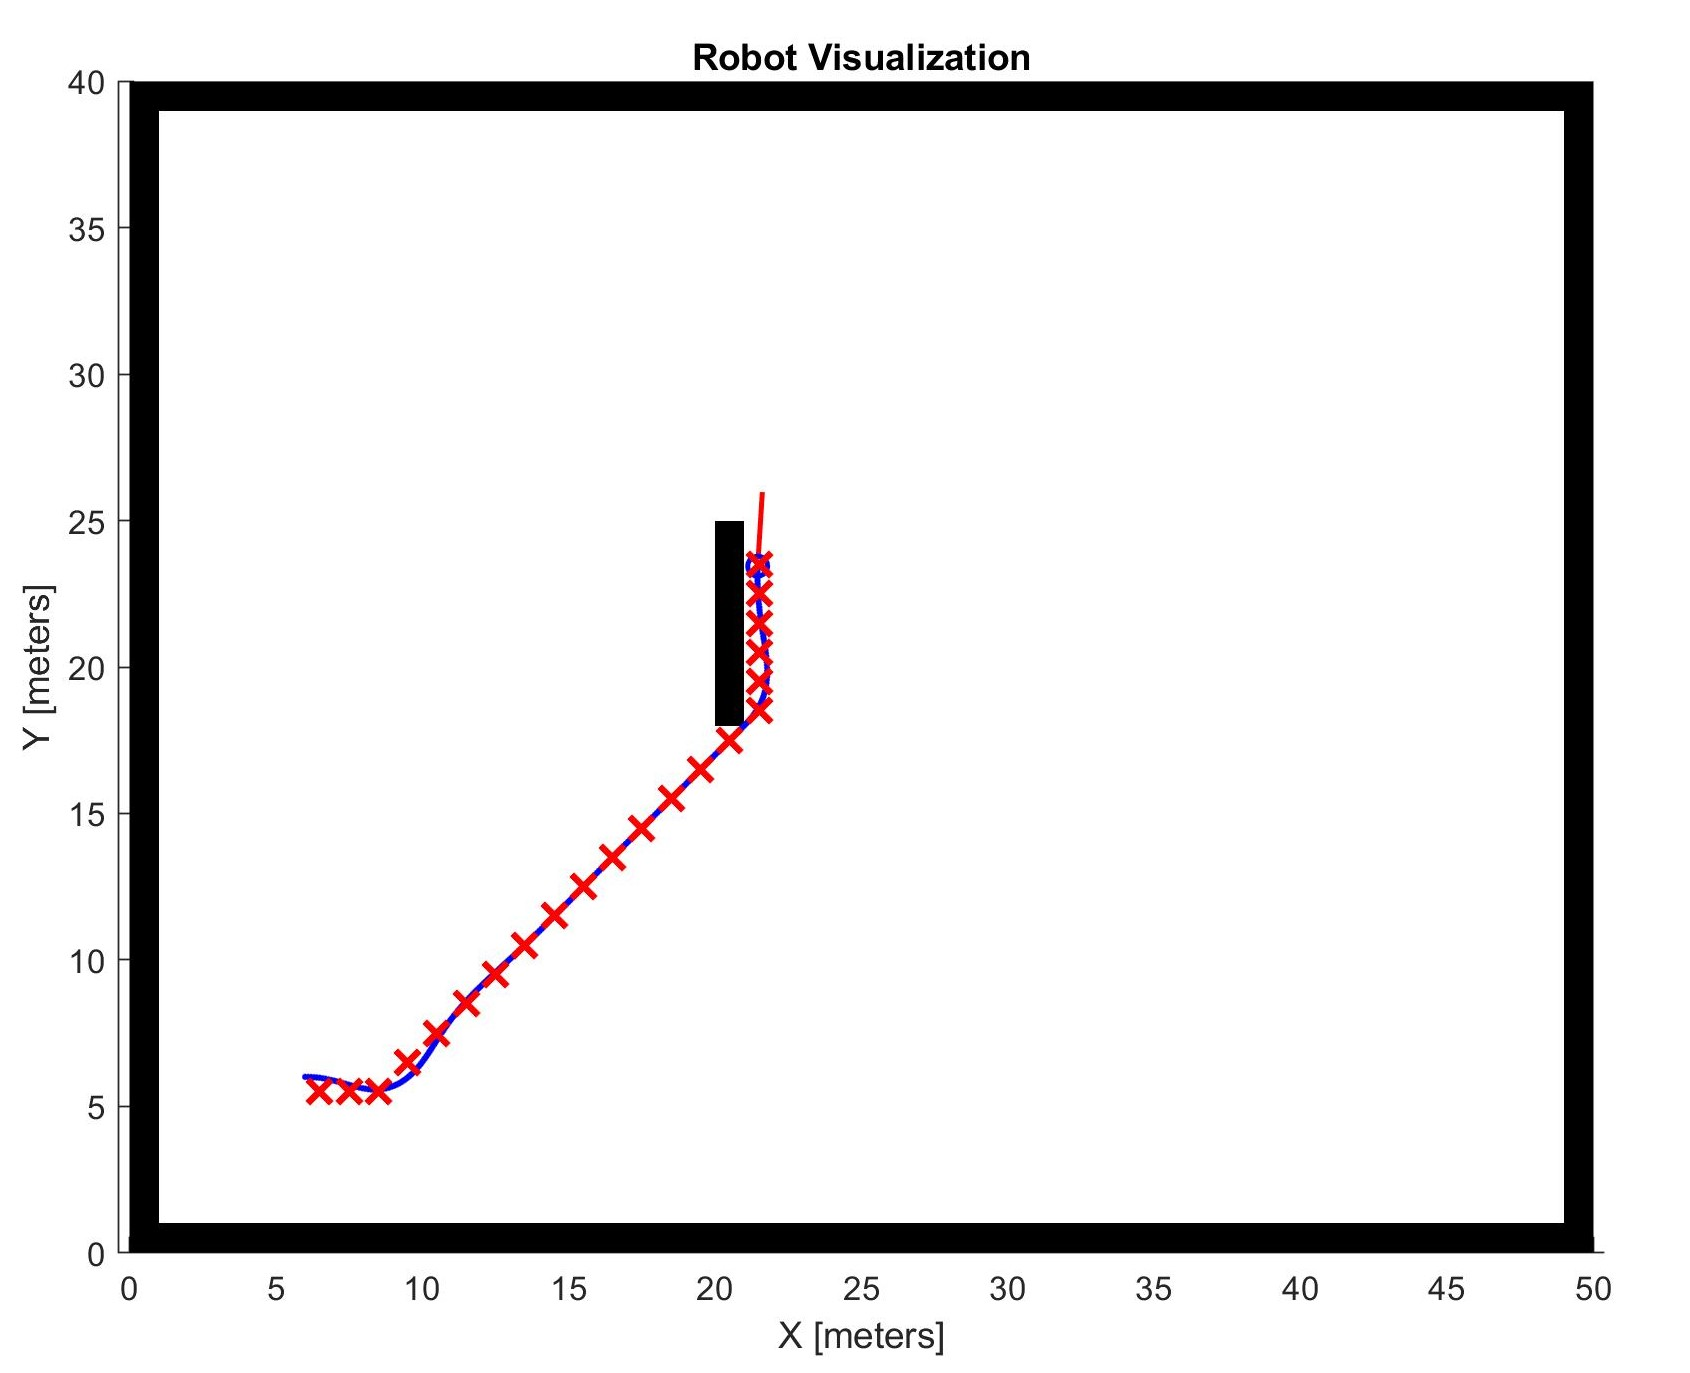
\includegraphics[scale=0.35]{Images/BFS path.jpg}
	\caption{مسیر پیشنهادی توسط الگوریتم $BFS$}\label{Fig BFS path}
\end{figure}

\begin{figure}[!h]
	\centering
	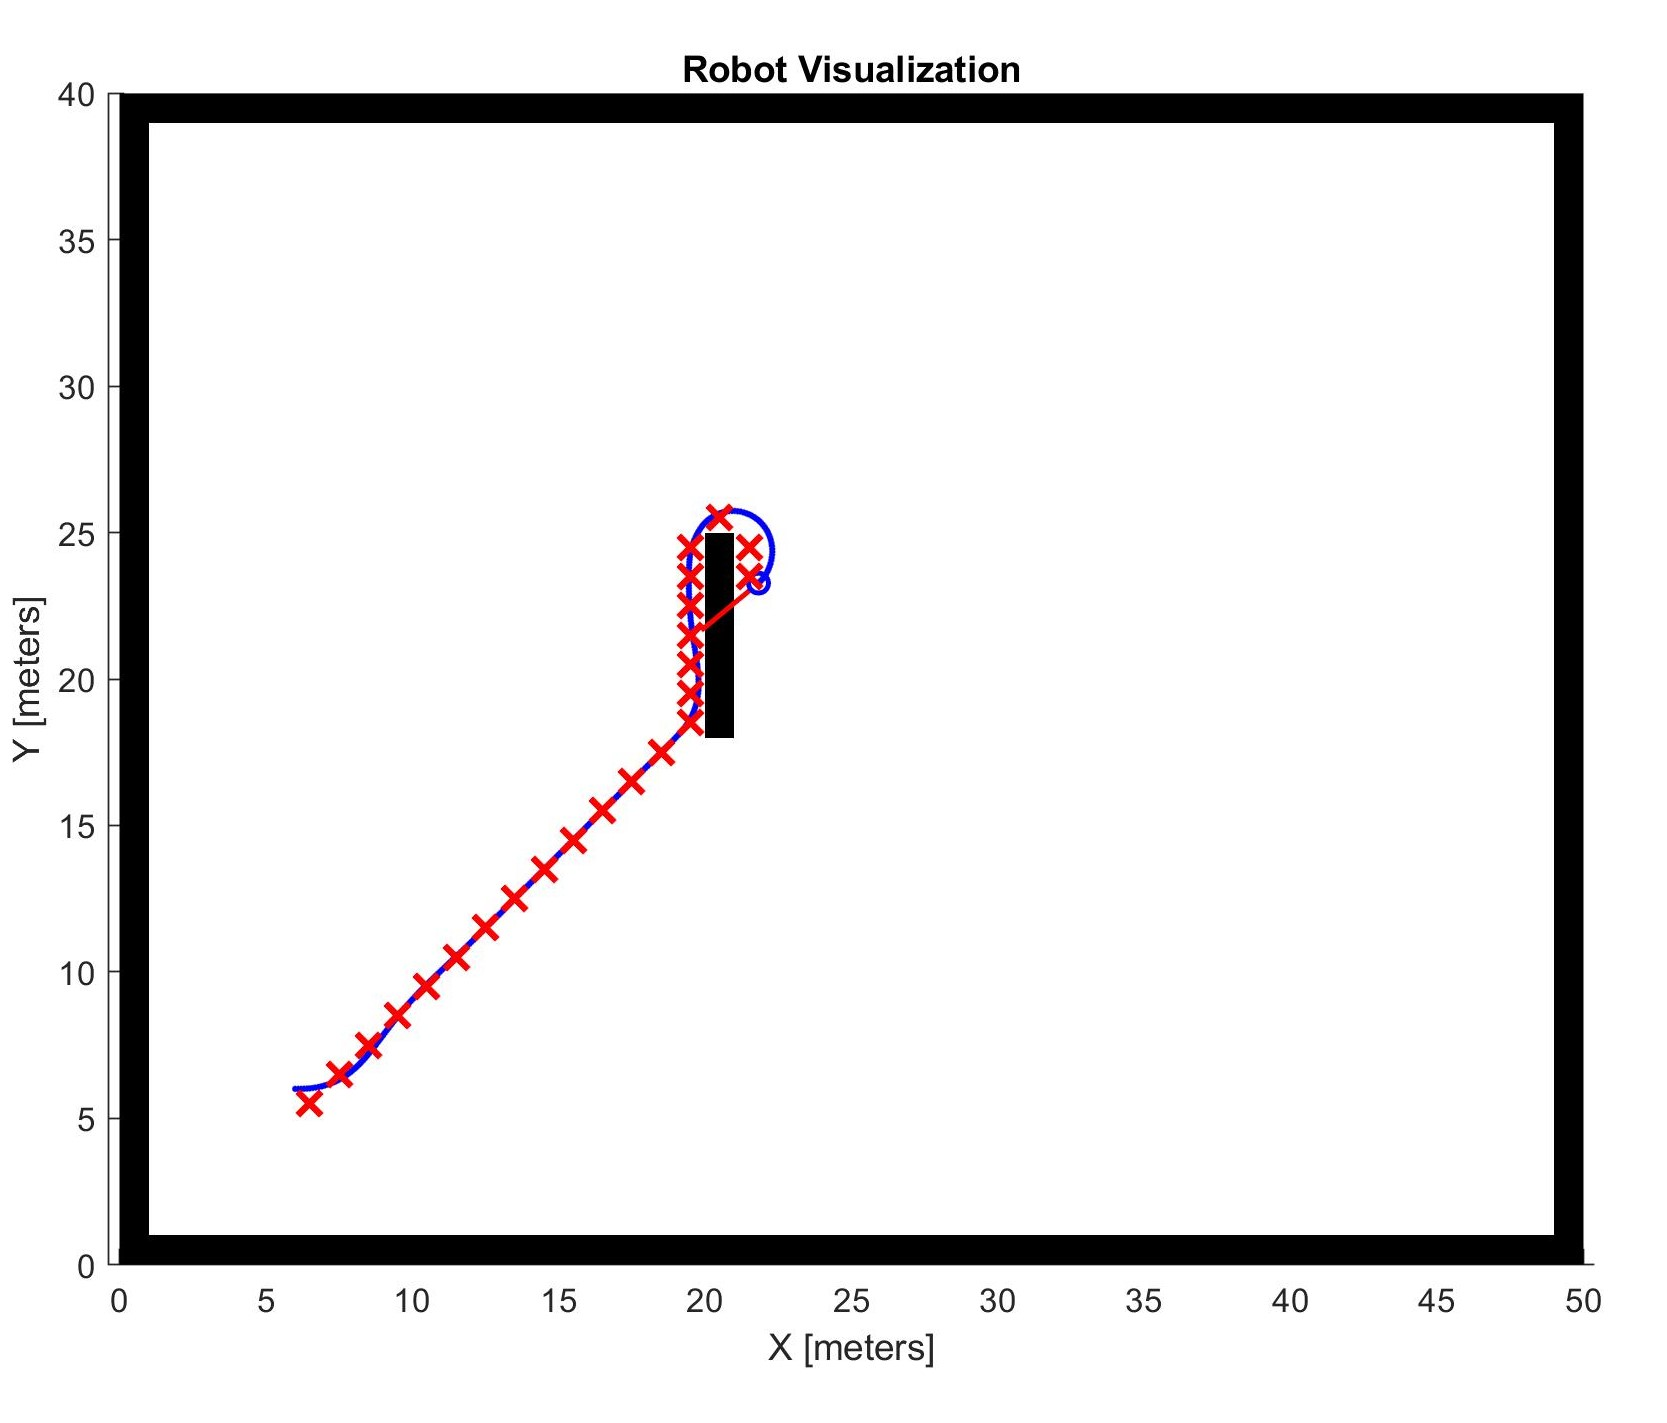
\includegraphics[scale=0.35]{Images/Greedy path.jpg}
	\caption{مسیر پیشنهادی توسط الگوریتم $search$ $best-first$ $Greedy$}\label{Fig Greedy path}
\end{figure}

\begin{figure}[!h]
	\centering
	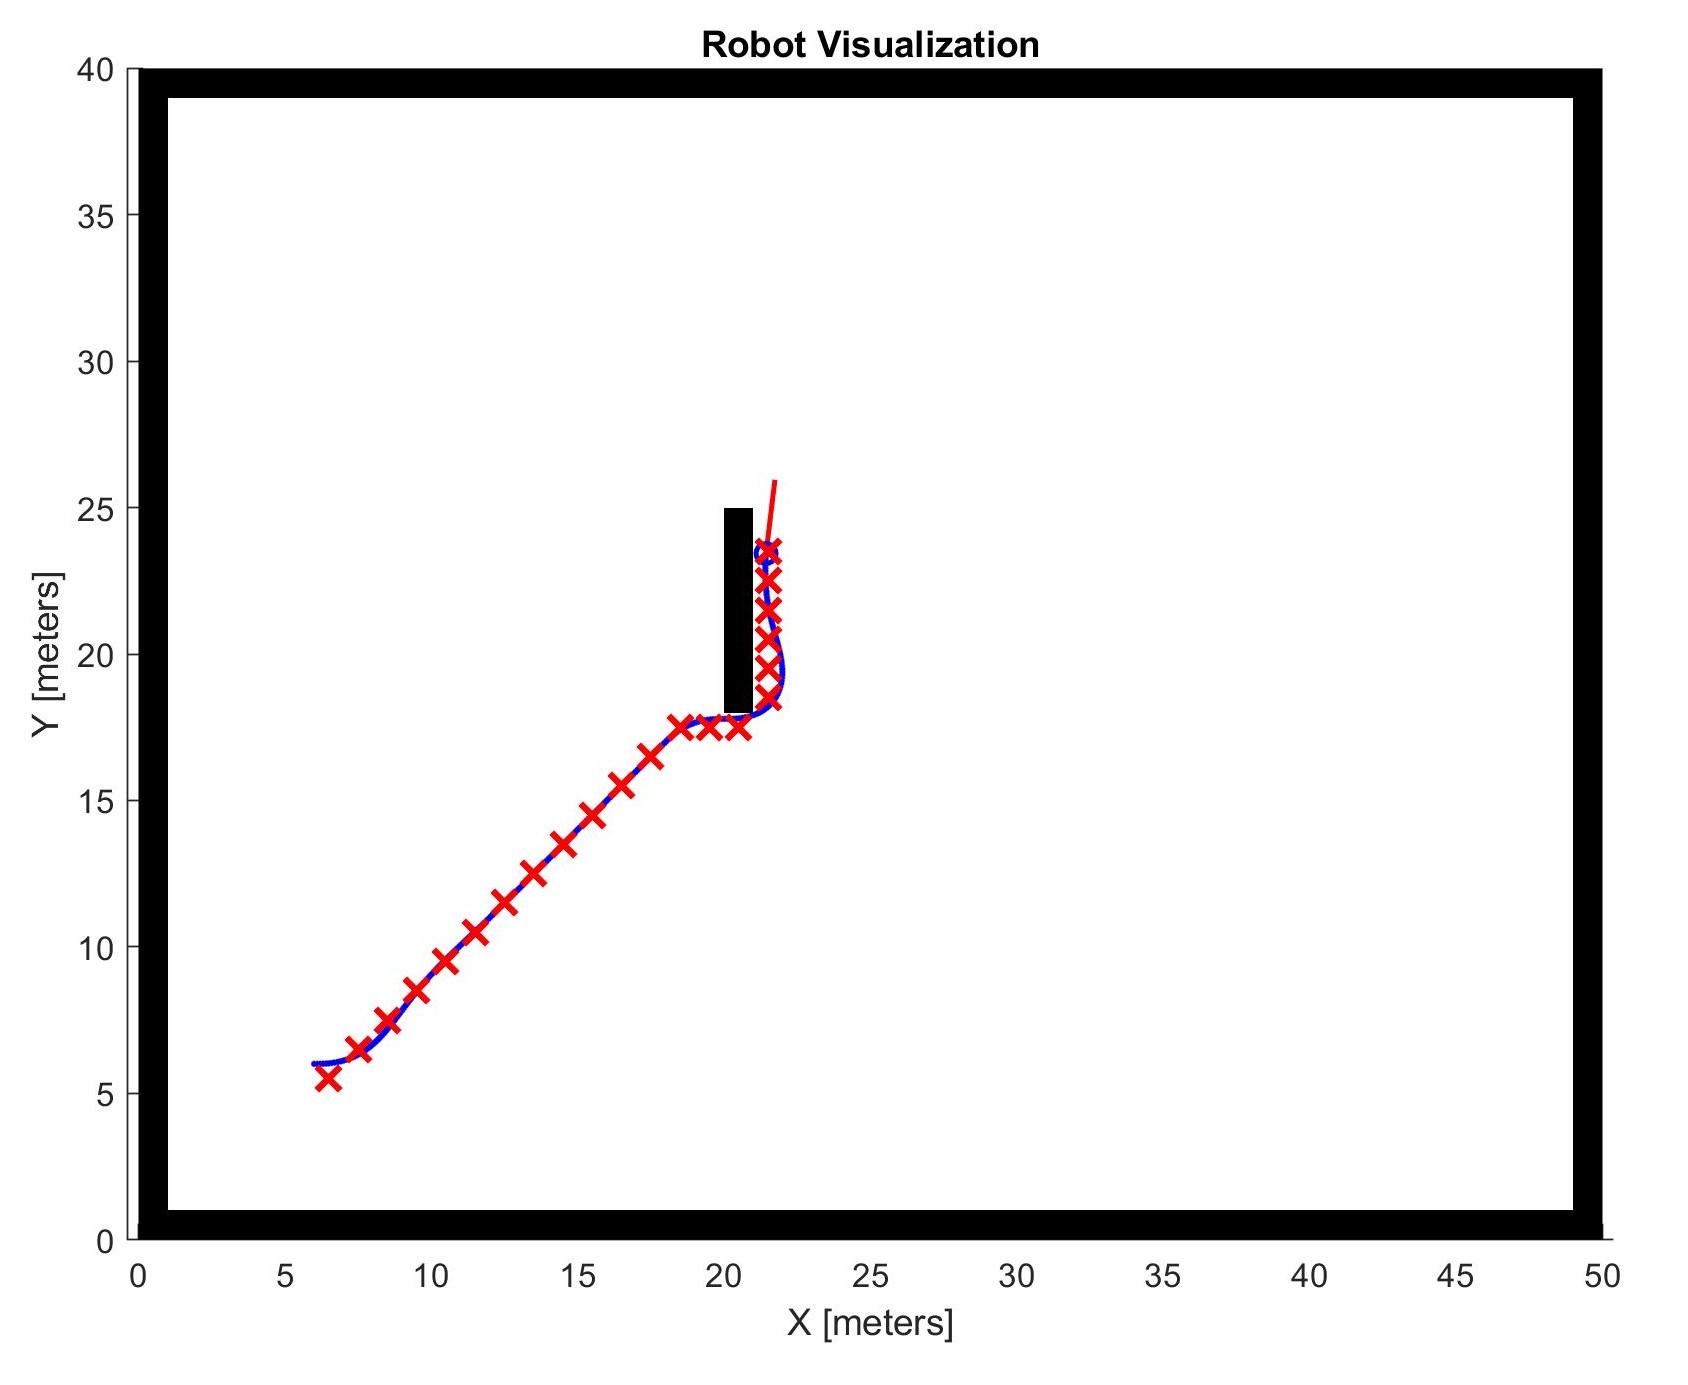
\includegraphics[scale=0.35]{Images/A-star path.jpg}
	\caption{مسیر پیشنهادی توسط الگوریتم $A^*$}\label{Fig A-star path}
\end{figure}

\newpage
همانطور که می‌شود دید در این مثال، الگوریتم، $search$ $best-first$ $Greedy$ مسیر طولانی‌تری نسبت به دو الگوریتم دیگر ارائه داده است. همچنین مسیرهای ارائه شده توسط دو الگوریتم، \verb|BFS| و $A^*$ هر دو بهین هستند.
\newpage
نکته دیگر قابل توجه، این است که هنگام چرخش به خصوص چرخش‌های سنگین همانند برگشت ربات در شکل \ref{Fig Greedy path} در بالای موانع، فشار زیادی به ربات آمده و کنترل مسیر برای او سخت بوده است. در نتیجه بهتر است کنترل‌کننده بهتری برای ربات در نظر گرفته شود. همچنین استفاده از الگوریتم‌هایی که سعی کنند میزان فشار وارده بر ربات را در تصمیمشان در نظر گرفته و کاهش دهند نیز، می‌تواند عضو کارهای آینده باشد.
\newpage
حال نوبت بررسی زمان مورد نیاز برای اجرای هر الگوریتم است. در این راستا، سه الگوریتم با نقاط تصادفی شروع و هدف، در حالی که برای هر سه یکسان باشند، اجرا گشتند. به ازای هر اندازه، 100 بار الگوریتم‌ها برای نقاط متفاوت بررسی و سپس از زمان آن‌ها میانگین گرفته شد. نتیجه در شکل \ref{Fig heuristic time} به نمایش در آمده است. همانطور که مشاهده می‌شود، زمان الگوریتم $A^*$ به مراتب بیشتر از الگوریتم‌های دیگر است. همچنین الگوریتم $search$ $best-first$ $Greedy$ کمترین زمان را دارد. در نتیجه هر چقدر بخواهیم به جواب معقولتری برسیم، مدت زمان بیشتر مورد نیاز است. در حالت کلی با توجه به اینکه برای 35000 نود، در کمتر از 200 میلی‌ثانیه برای الگوریتم $A^*$ به جواب رسیده است، استفاده از این الگوریتم توصیه می‌شود. قابل ذکر است که الگوریتم $A^*$ روش معقول‌تری نسبت به دو الگوریتم دیگر دارد و همچنین عملکرد آن در شرایطی که وزن‌ یال‌ها نسبت به هم بسیار متفاوت باشند بهتر نیز خواهد بود و قابلیت تعمیم به مسائل دیگر را نیز دارد.

\begin{figure}[!h]
	\centering
	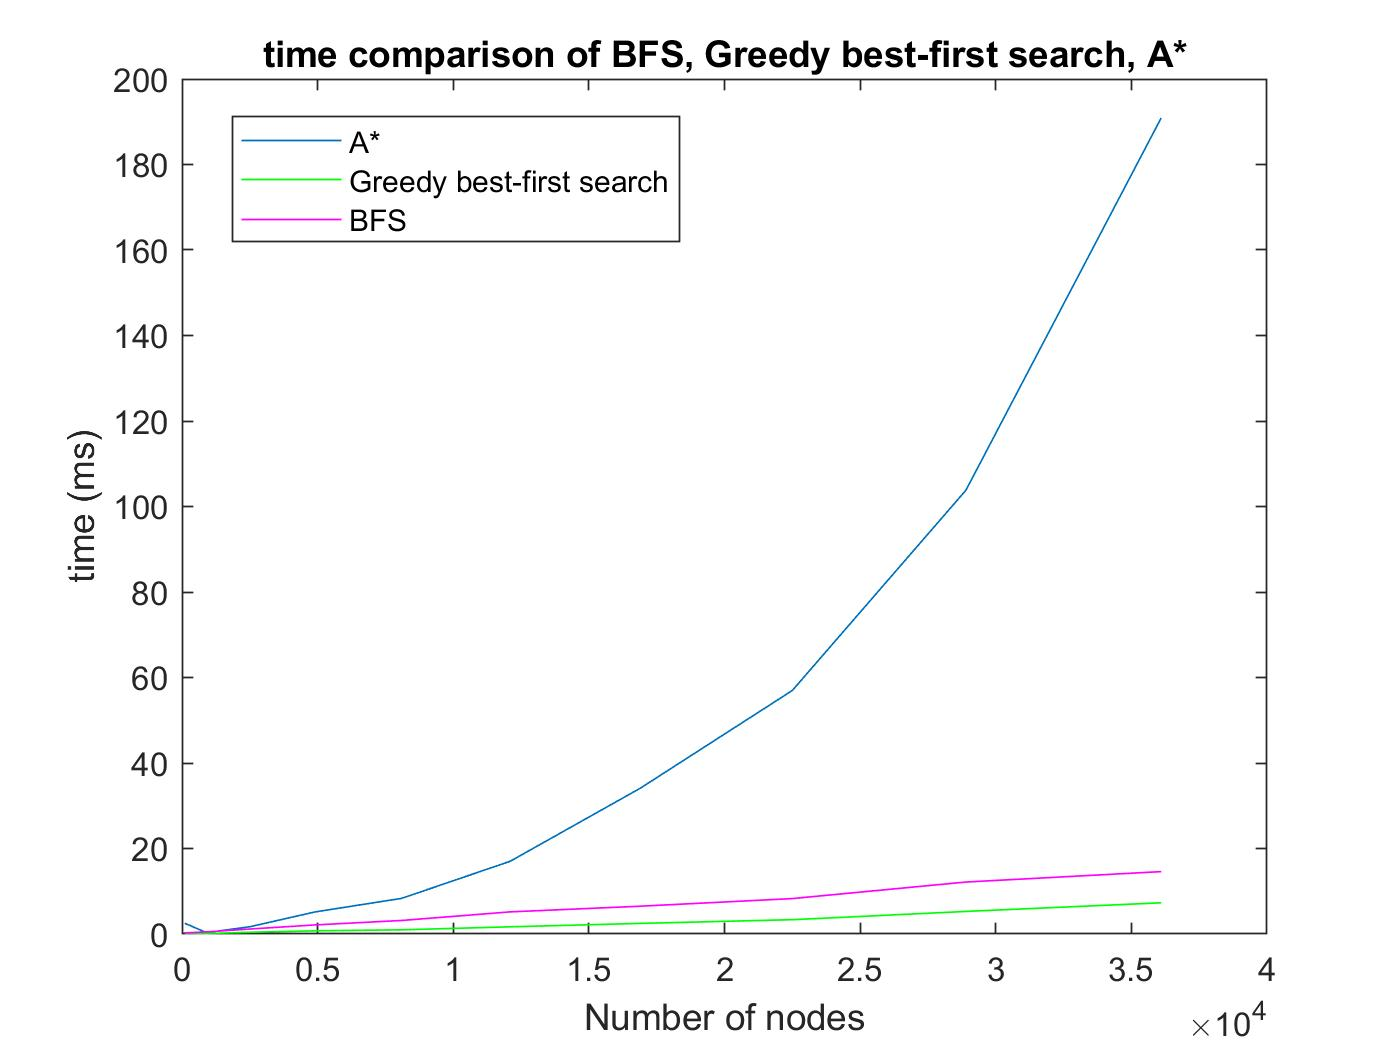
\includegraphics[scale=0.35]{Images/Heuristic time.jpg}
	\caption{مقایسه زمانی سه الگوریتم $BFS$، $search$ $best-first$ $Greedy$ و $A^*$}\label{Fig heuristic time}
\end{figure}


\newpage
\section{$Q-learning$}


















\chapter{مسیریابی برای اجماع ربات‌ها}
%%%%%%%%%%%%%%%%%%%%%%%%%%%%%%%%%%%%%%%%%%%
\section{مقدمه}
در این قسمت به پیاده‌سازی الگوریتم‌های فصل \ref{ch path planning} برای اجماع ربات‌ها به صورت آنلاین پرداخته می‌شود. منظور از آنلاین بودن برنامه‌ریزی این است که در هر گام زمانی، ربات مجددا الگوریتم مسیریابی را اجرا نماید. برای مسیریابی با میدان پتانسیل، در ابتدا اجماع با شکل‌دهی ثابت برای عبور از موانع تلاش می‌کند اما پس از اشاره به ایرادات این روش، در ادامه کار شکل‌گیری پلتون شکسته و دوباره به شکل‌گیری تلاش خواهند کرد. همچنین موانع به صورت ثابت و متحرک خواهند بود.

\section{میدان پتانسیل}
در این قسمت تمامی مسیریابی‌ها تنها با میدان پتانسیل انجام شده است. در ابتدا شکل‌گیری ثابت و سپس شکل‌گیری با قابلیت شکسته شدن مورد بررسی قرار خواهد گرفت. قابل ذکر است که در هر دو روش تا جای ممکن محاسبات به صورت نامتمرکز\LTRfootnote{distributed} بوده است.

\subsection{جلوگیری از برخورد با موانع با شکل‌گیری ثابت}
در این قسمت یک شکل‌گیری ثابت برای دسته ربات‌ها در نظر گرفته شده است. ایده اصلی این است که نیروی جاذبه برای رهبر که در مرکز دسته پلتون حضور دارد و نیروی دافعه برای هر ربات محاسبه گردد و در نهایت نیروی کلی به دست آید. در این راستا برای محاسبه دو ایده برای پیاده‌سازی به وجود می‌آید اول اینکه همانند شکل \ref{Fig platoon-potential-field-simulink} به صورت متمرکز تمام داده‌ها به محاسبه‌گری که مسئول محاسبه مسیر ربات رهبر است فرستاده شود و نیروهای دافعه و جاذبه در آن محاسبه گردند.
\begin{figure}[!h]
	\centering
	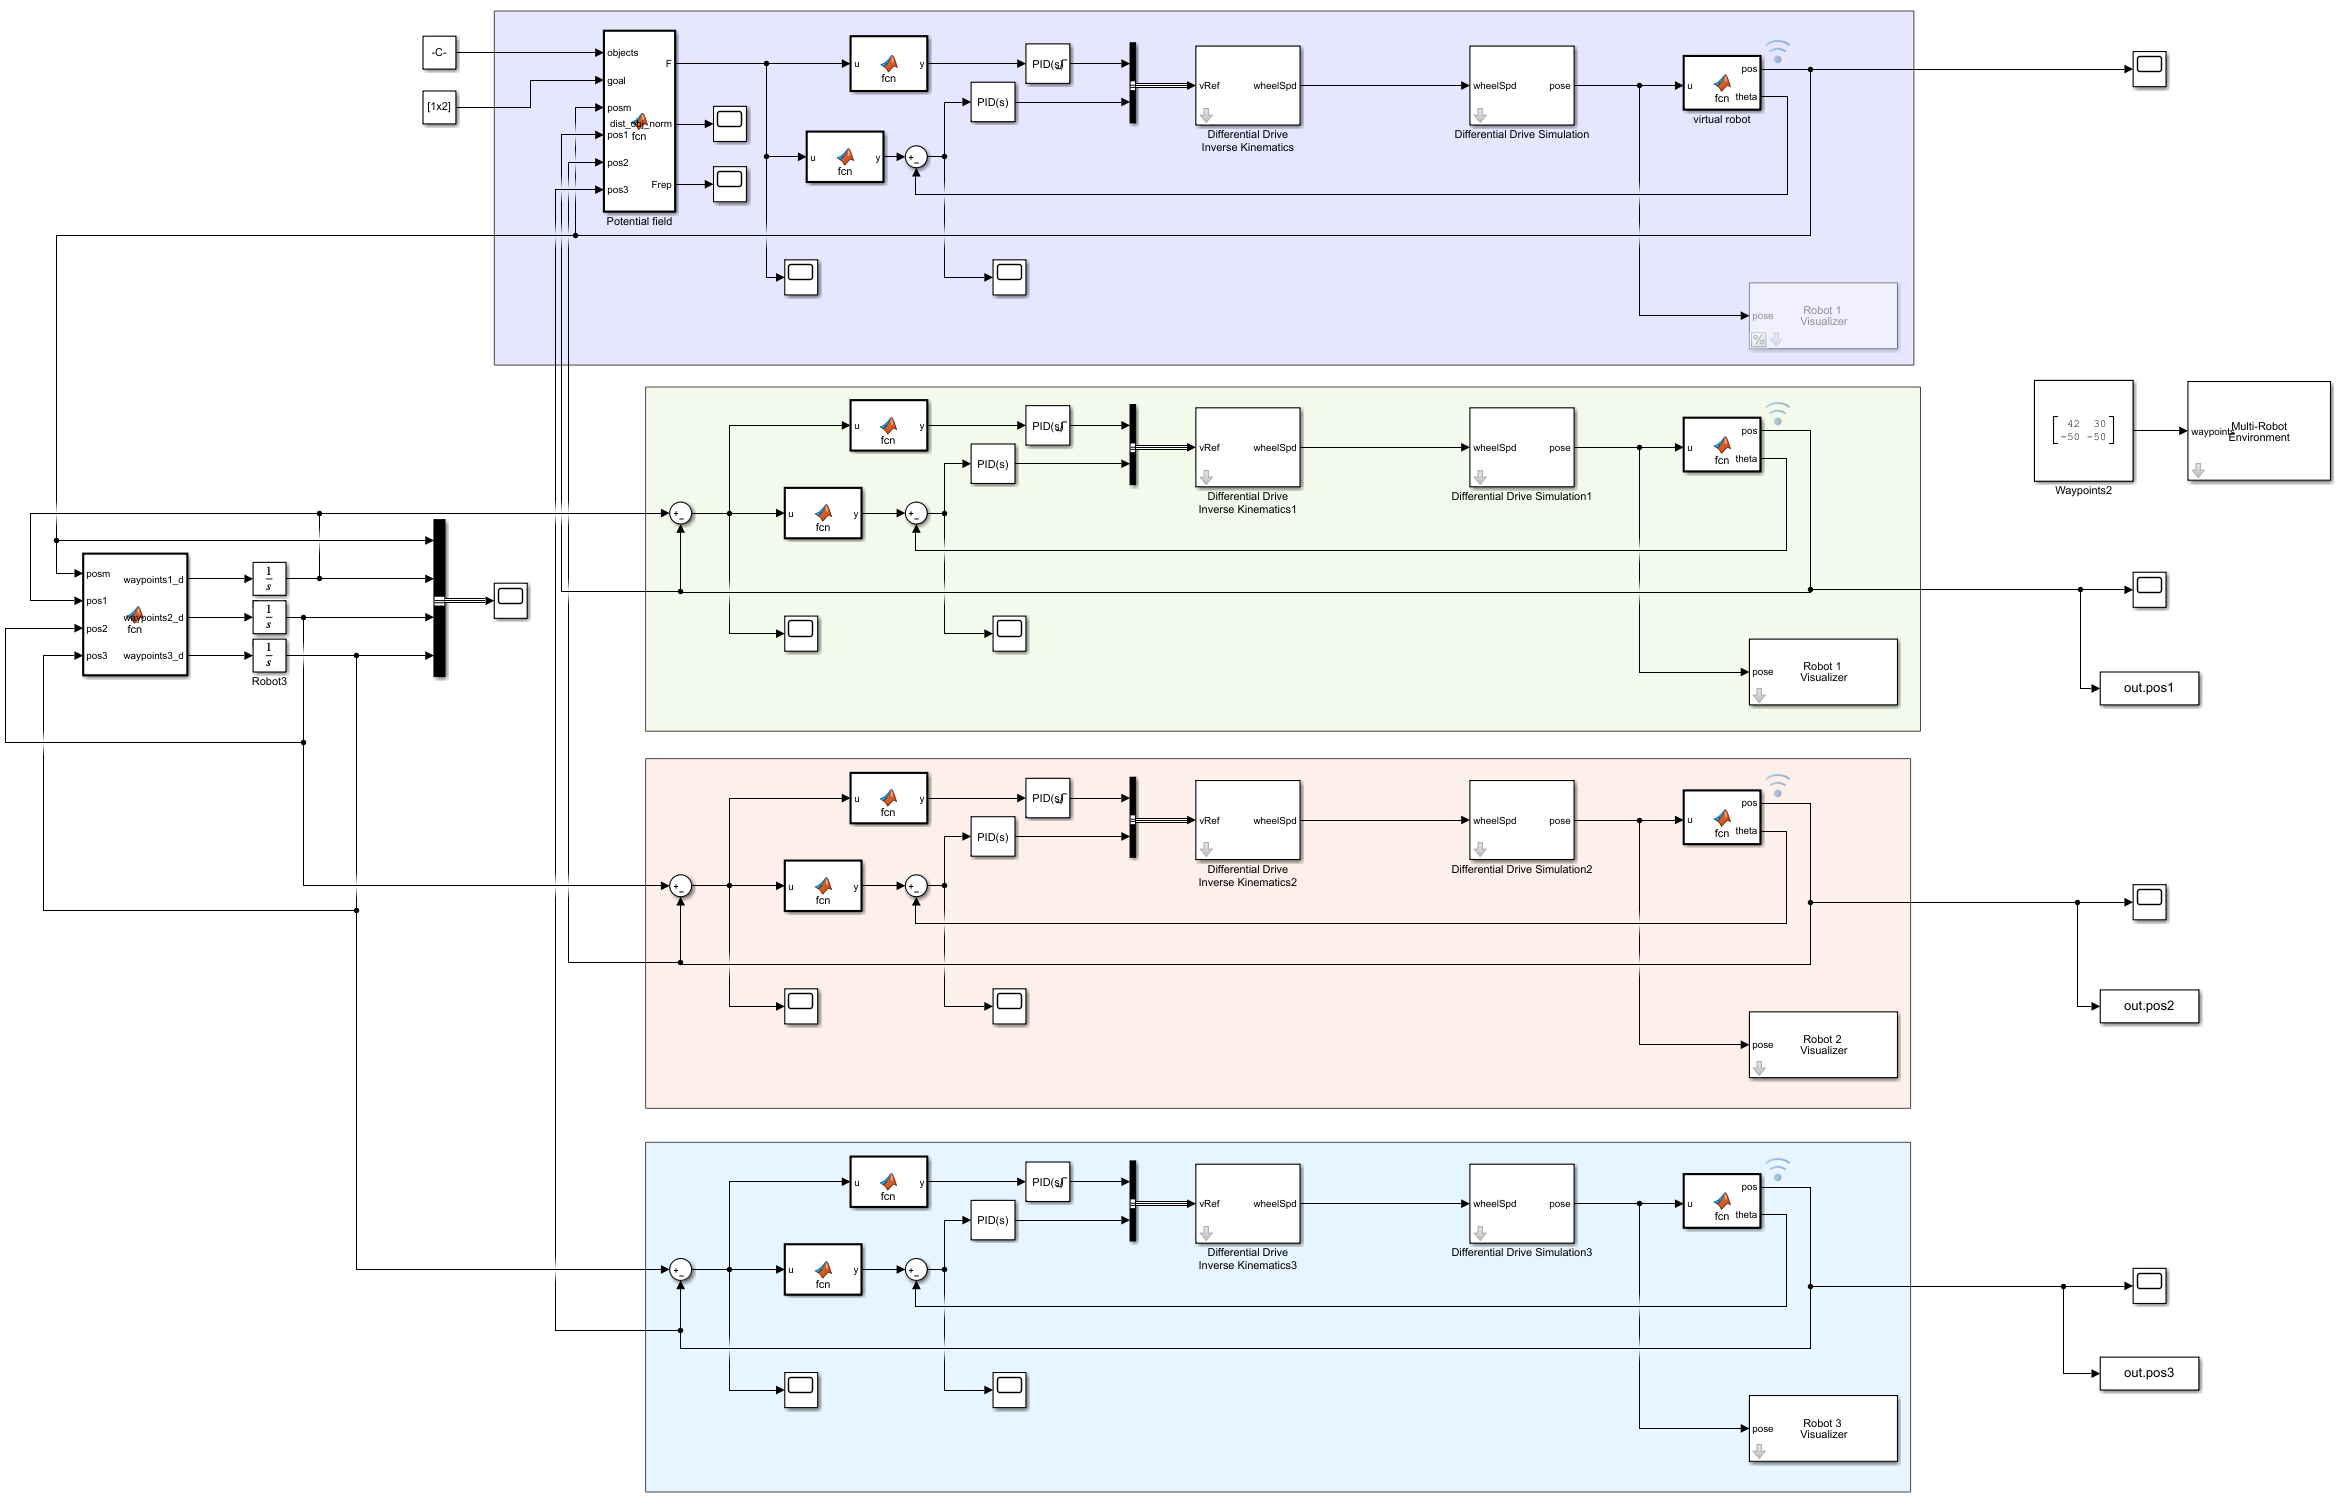
\includegraphics[scale=0.25]{Images/platoon-potential-field-simulink.png}
	\caption{بلوک‌های شبیه‌سازی در روش شکل‌گیری ثابت با محاسبات متمرکز}\label{Fig platoon-potential-field-simulink}
\end{figure}


مکان ربات‌ها برای روش متمرکز به رنگ‌های سبز، آبی و قرمز و موانع با رنگ سیاه در شکل \ref{Fig platoon-potential-field-pos} به نمایش در آمده است.
\begin{figure}[!h]
	\centering
	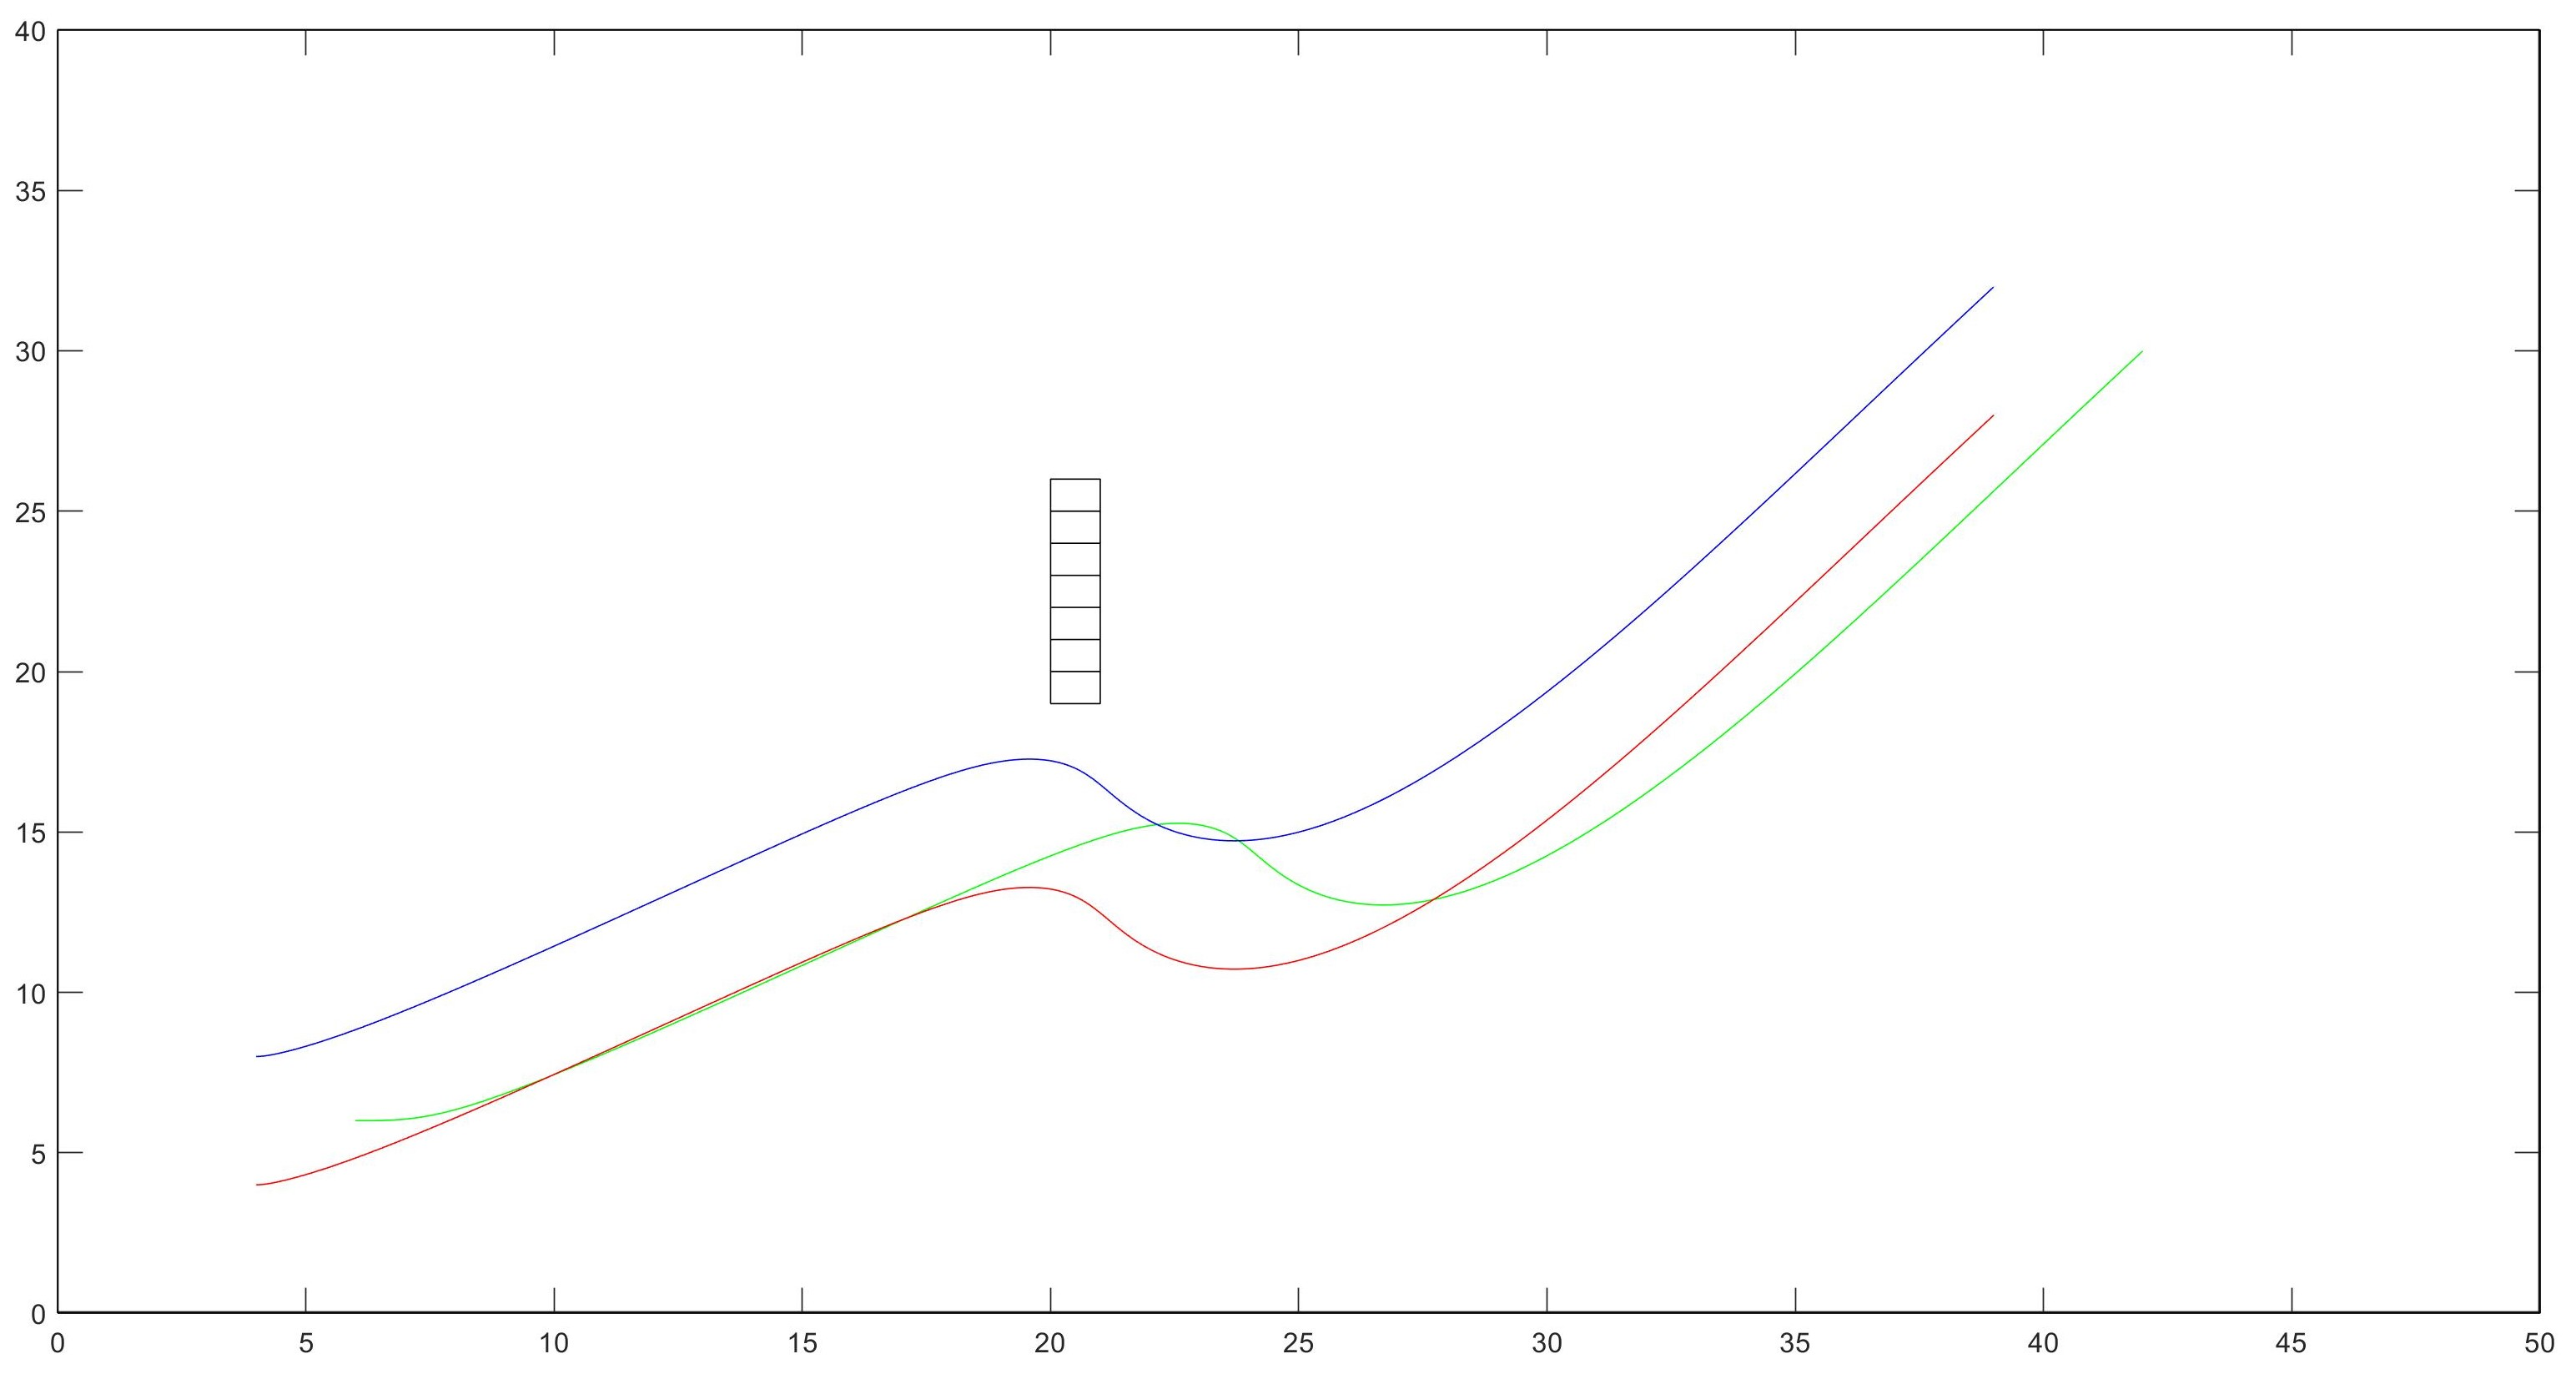
\includegraphics[scale=0.2]{Images/platoon-potential-field-pos.jpg}
	\caption{مکان ربات‌ها در روش شکل‌گیری ثابت با محاسبات متمرکز}\label{Fig platoon-potential-field-pos}
\end{figure}

در روش دوم، برای اینکه دوره محاسبات کاهش یابد، همانند شکل \ref{Fig platoon-potential-field-distributed-simulink} محاسبه نیروی دافعه ناشی از هر ربات، به صورت نامتمرکز و جداگانه در هر ربات محاسبه می‌شود و سپس به ربات رهبر فرستاده می‌شود. محاسبه‌گر ربات رهبر تنها مقادیر را با هم جمع می‌نماید تا به نیروی دافعه برسد. اما نیروی جاذبه همچنان توسط رهبر محاسبه می‌گردد.
\begin{figure}[!h]
	\centering
	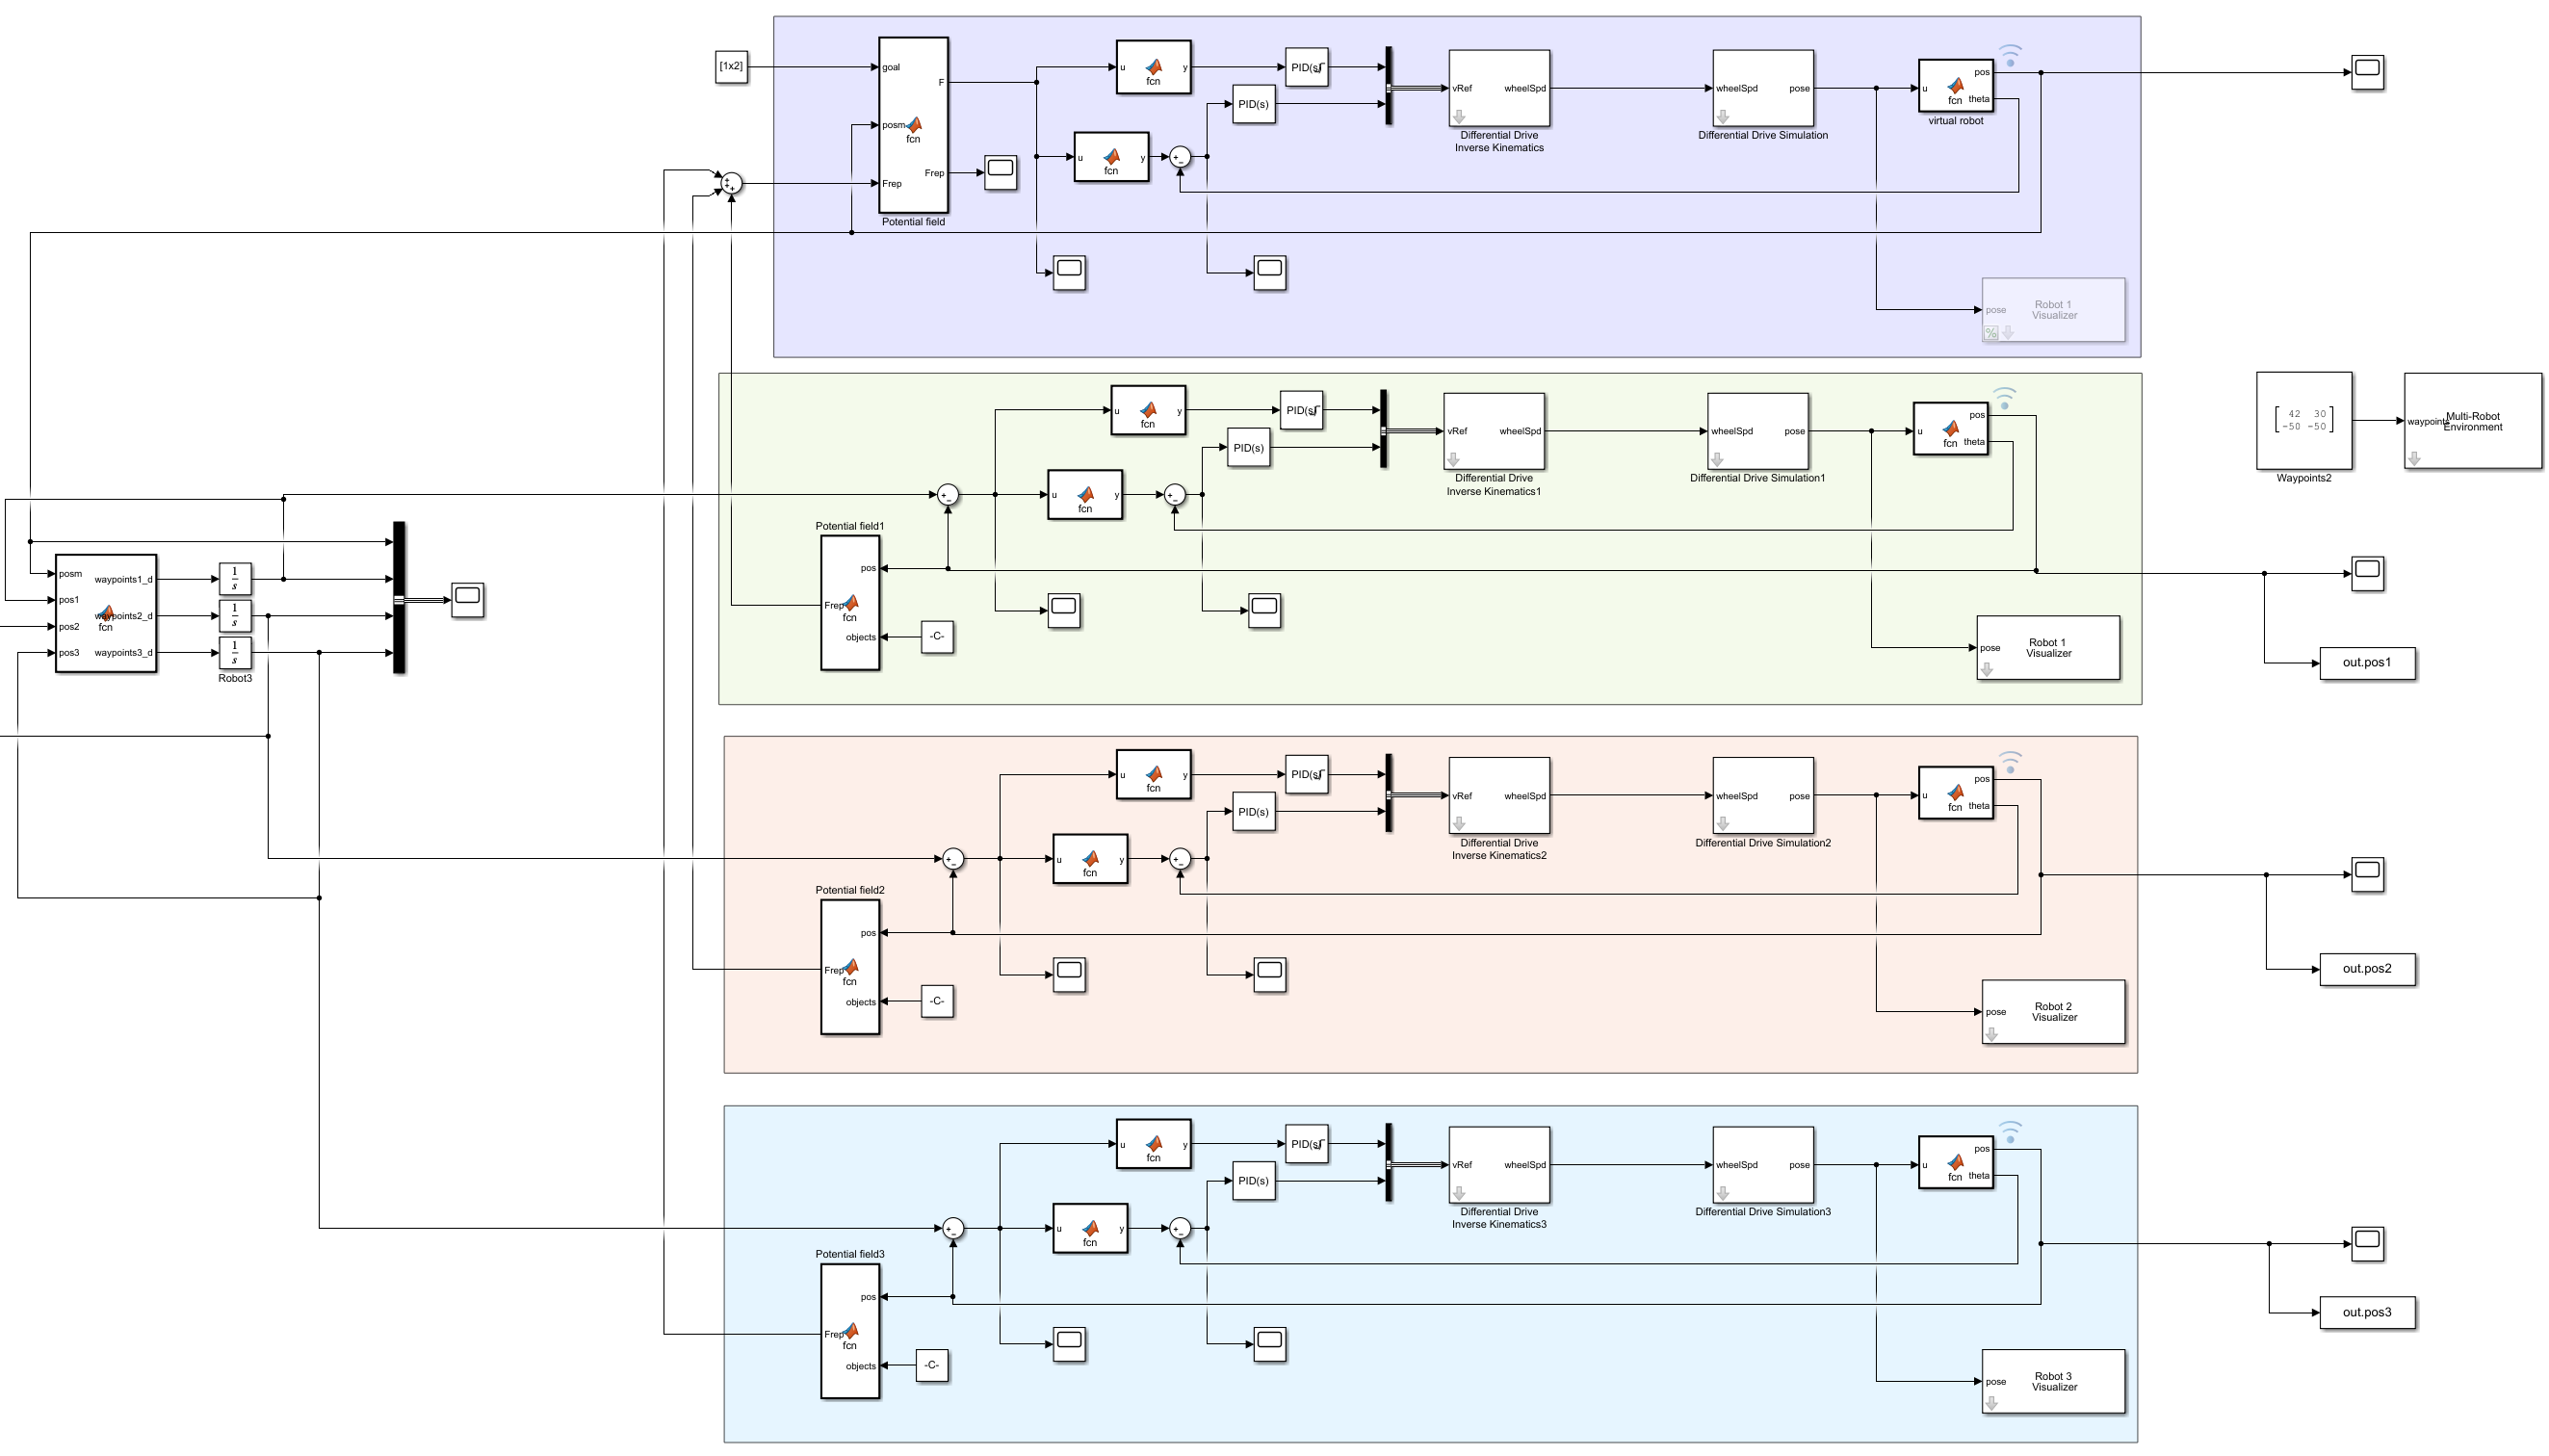
\includegraphics[scale=0.25]{Images/platoon-potential-field-distributed-simulink.png}
	\caption{بلوک‌های شبیه‌سازی در روش شکل‌گیری ثابت با محاسبات نامتمرکز}\label{Fig platoon-potential-field-distributed-simulink}
\end{figure}


مکان ربات‌ها برای روش نامتمرکز در شکل \ref{Fig platoon-potential-field-distributed-pos} به نمایش در آمده است.
\begin{figure}[!h]
	\centering
	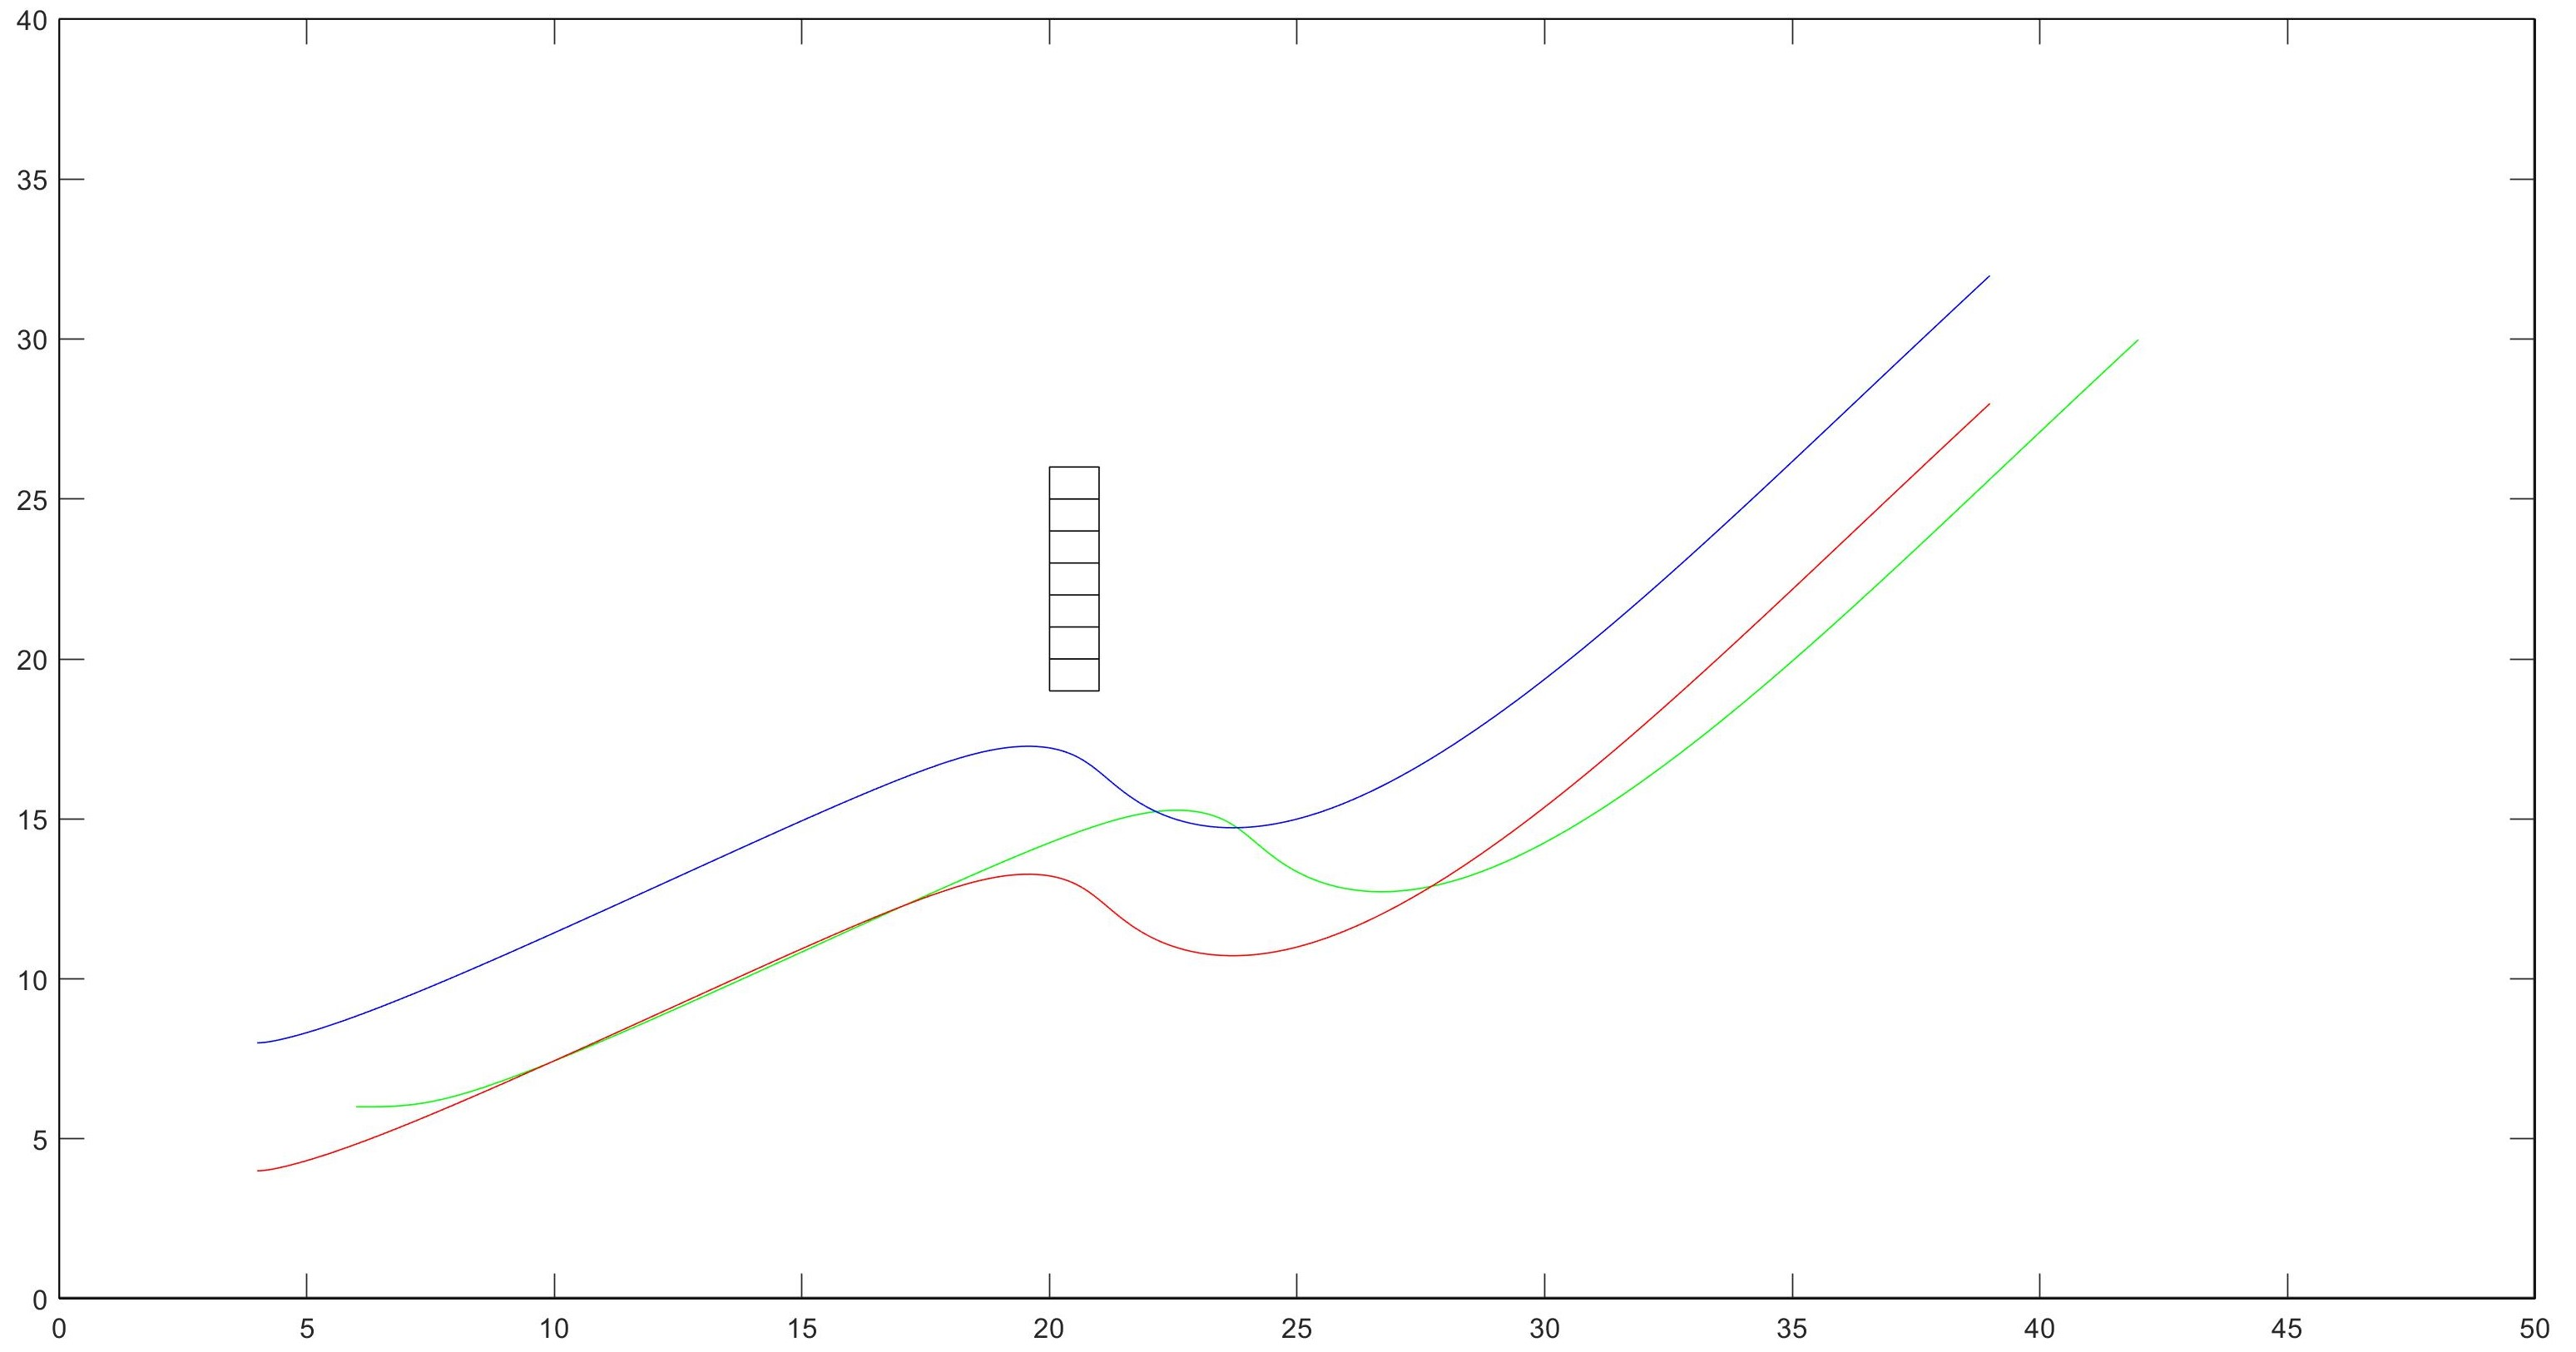
\includegraphics[scale=0.2]{Images/platoon-potential-field-distributed-pos.jpg}
	\caption{مکان ربات‌ها در روش شکل‌گیری ثابت با محاسبات نامتمرکز}\label{Fig platoon-potential-field-distributed-pos}
\end{figure}


مشکل اصلی این روش این است که امکان دارد هر ربات از جهت مختلفی به طور همزمان به مانع نزدیک شوند، مخصوصا در شرایطی که مانع متحرک باشد، لذا نیاز داریم هر ربات به تنهایی میدان پتانسیل مخصوص به خود را داشته باشد. که در قسمت بعد این ایده پیاده‌سازی گشته است.

\subsection{جلوگیری از برخورد با موانع با شکل‌گیری شکننده}\label{sec potential-field for every robot}
در این روش هر ربات با میدان پتانسیل مخصوص به خود مسیریابی را انجام می‌دهد و نقطه‌ای که در هر لحظه باید در اجماع قرار گیرد به عنوان نقطه هدف در نظر گرفته می‌شود. بلوک‌های شبیه‌سازی در شکل \ref{Fig platoon-potential-field-independent-simulink} و نتیجه حرکت ربات‌ها در شکل \ref{Fig platoon-potential-field-independent-pos} به نمایش در آمده است.
\begin{figure}[!h]
	\centering
	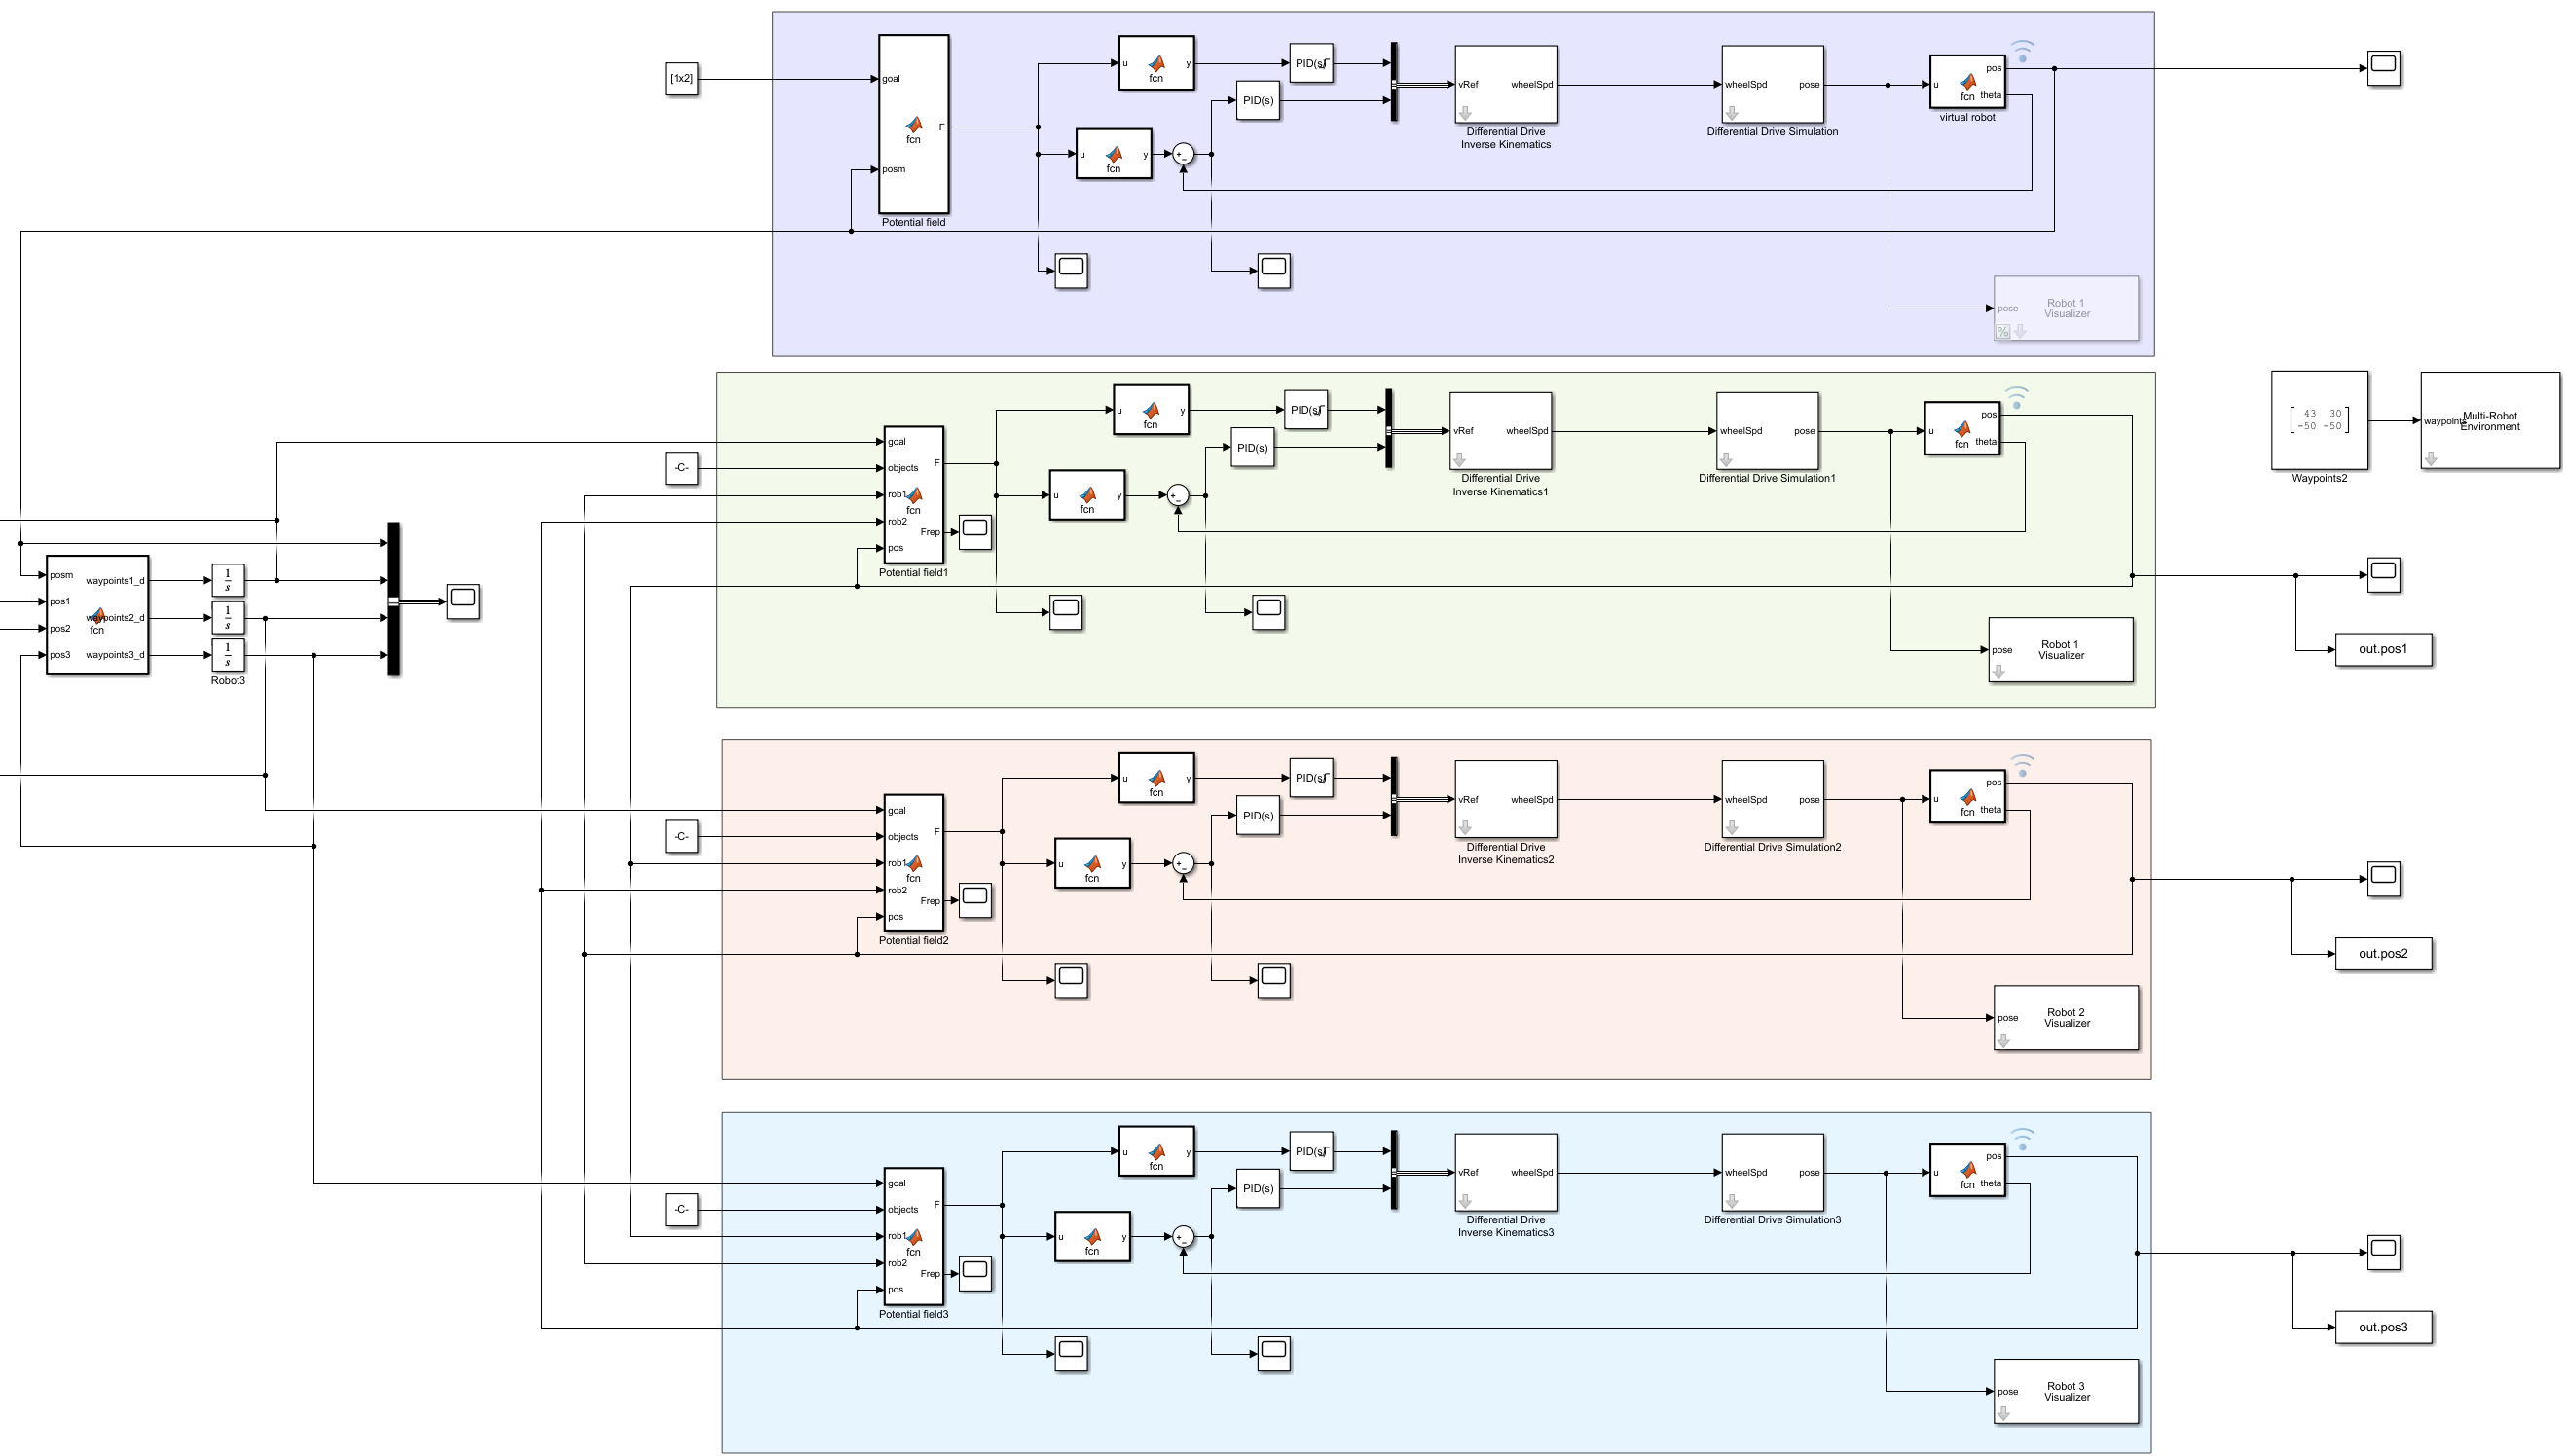
\includegraphics[scale=0.2]{Images/platoon-potential-field-independent-simulink.png}
	\caption{بلوک‌های شبیه‌سازی در روش شکل‌گیری شکننده}\label{Fig platoon-potential-field-independent-simulink}
\end{figure}

\begin{figure}[!h]
	\centering
	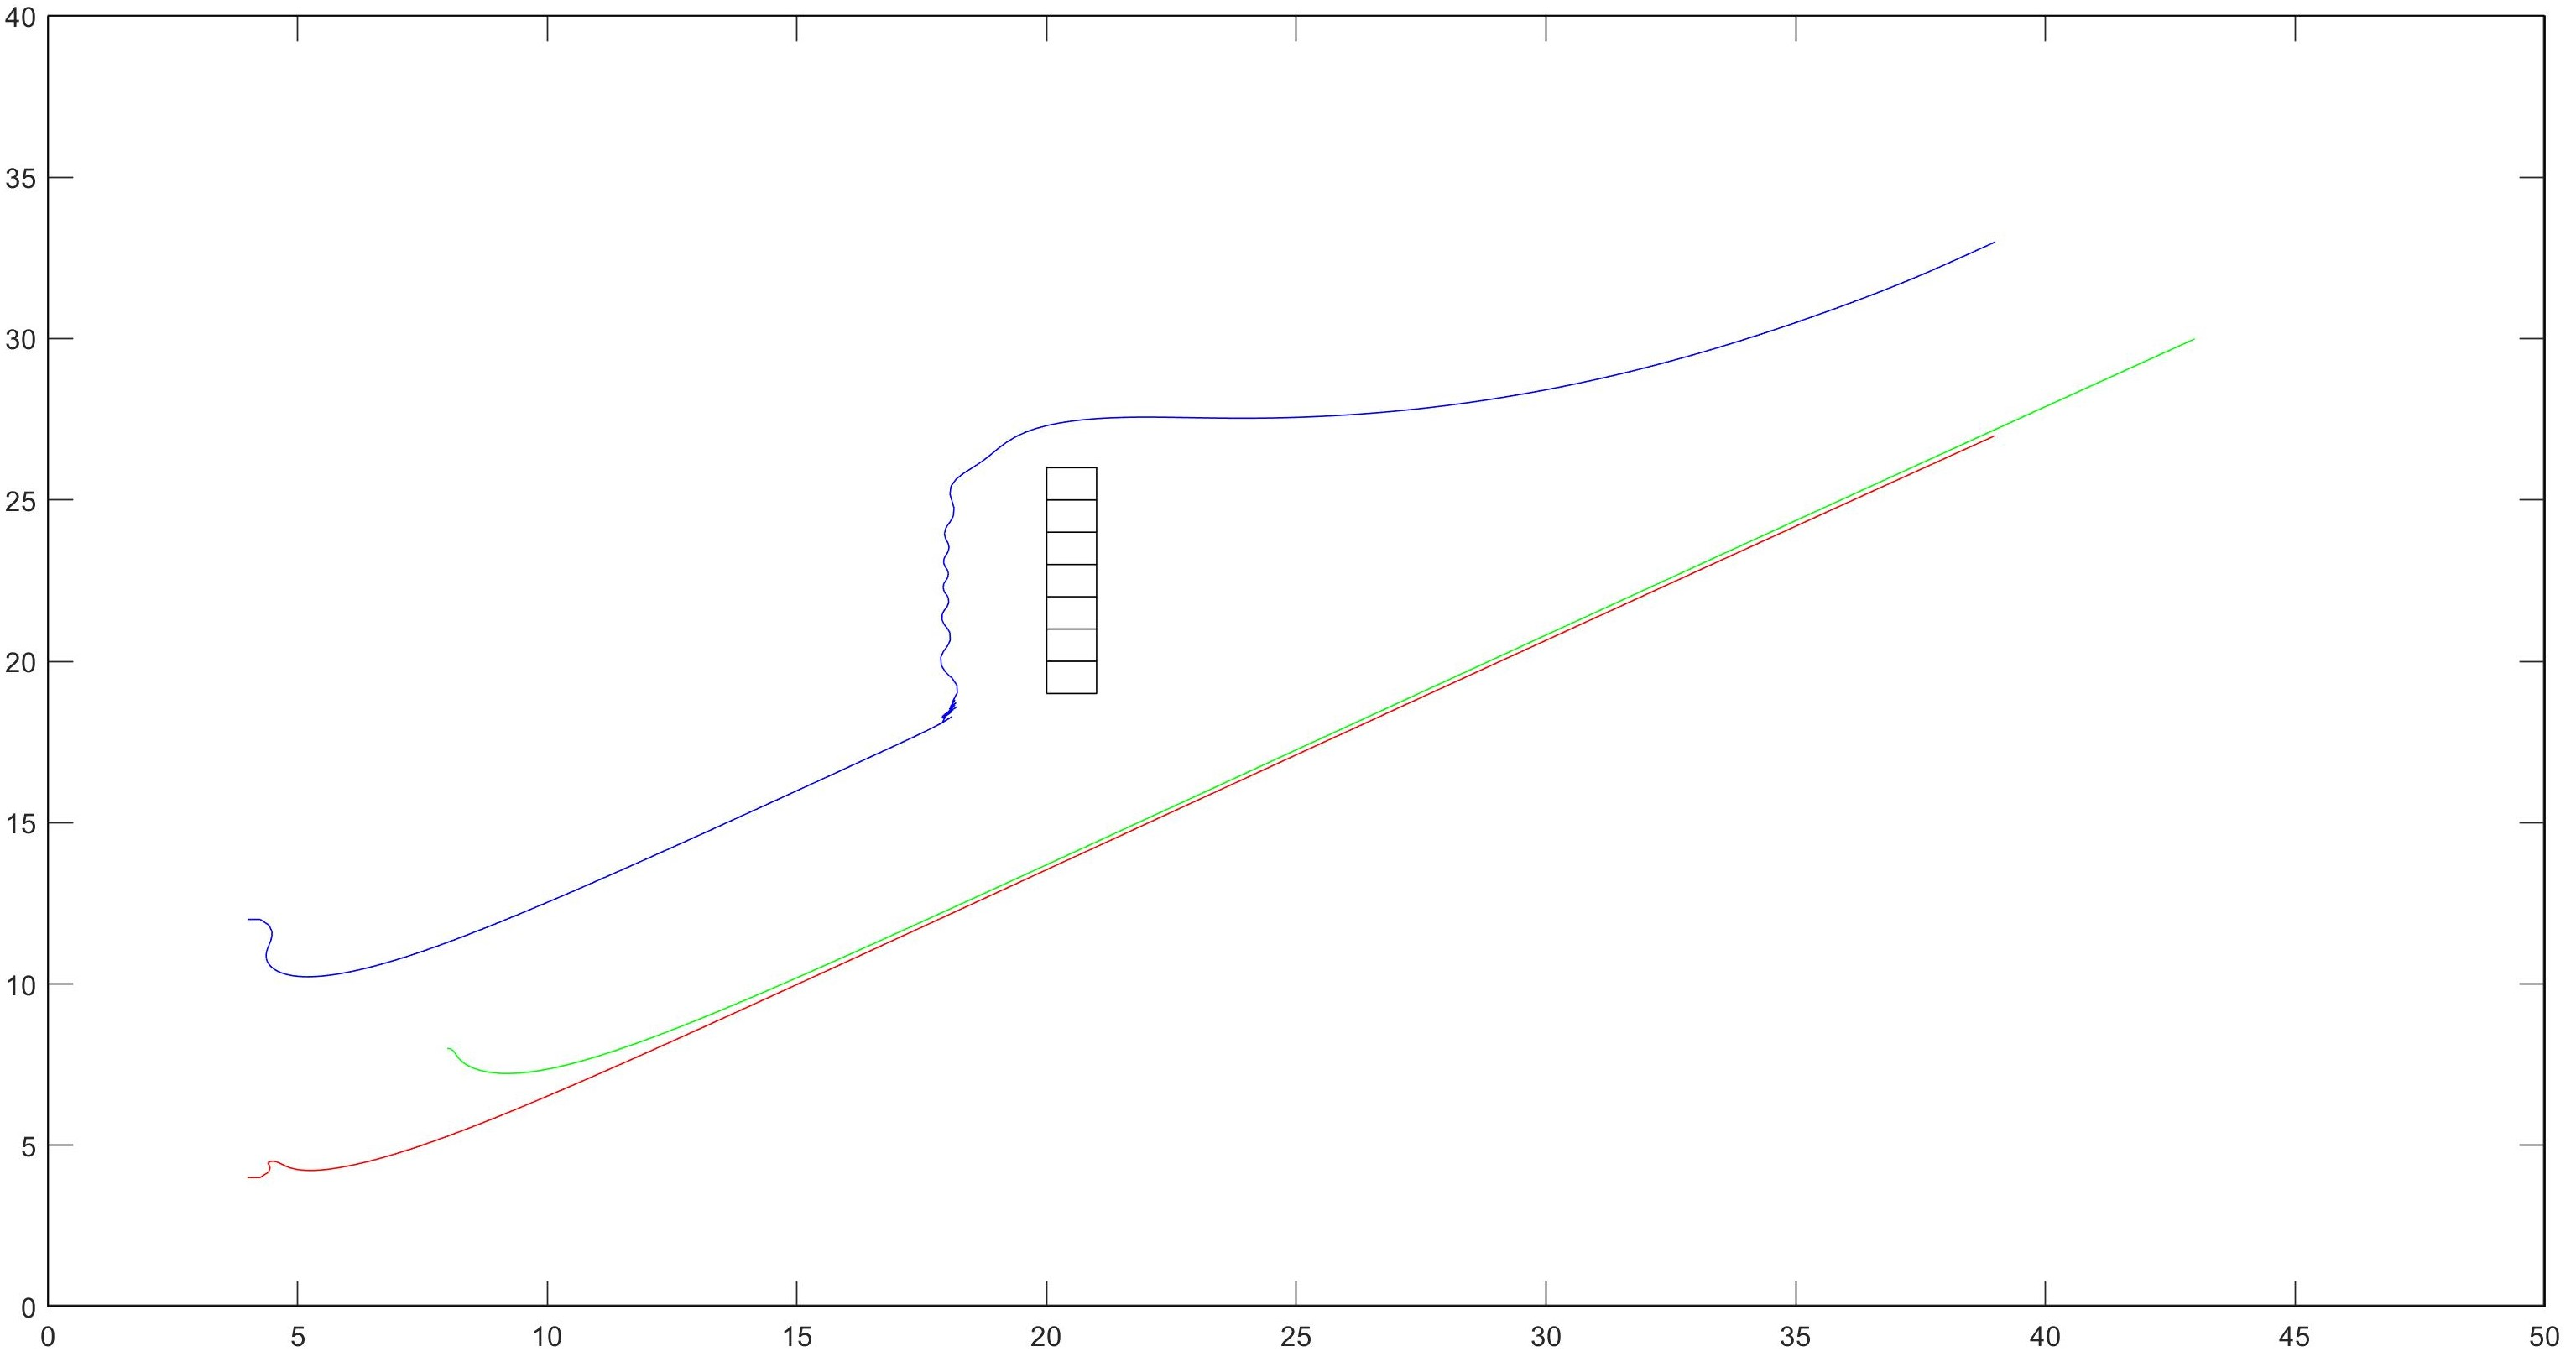
\includegraphics[scale=0.2]{Images/platoon-potential-field-independent-pos.jpg}
	\caption{مکان ربات‌ها در روش شکل‌گیری شکننده}\label{Fig platoon-potential-field-independent-pos}
\end{figure}



\section{روش‌های ابتکاری}
در این قسمت روش‌های ابتکاری فصل \ref{ch path planning} پیاده‌سازی شده‌اند. این مسیریابی‌ها به صورت آنلاین انجام شده است تا از برخورد با موانع متحرک نیز بتوان اجتناب کرد. روش پیاده‌سازی به این صورت است که در عامل رهبر، این مسیریابی انجام و ربات طبق آن حرکت می‌نماید. سایر ربات‌ها همانند بخش \ref{sec potential-field for every robot} از میدان پتانسیل برای رسیدن به مکان مطلوب تعیین شده از طرف کنترل‌کننده پلتون و دوری از موانع به صورت انفرادی، استفاده می‌کنند.

\subsection{\lr{BFS}}
نحوه پیاده‌سازی مسیریابی \lr{BFS} توسط اجماع ربات‌ها در شکل \ref{Fig platoon-BSF-simulink} و مسیر پیموده شده در شکل \ref{Fig platoon-BSF-pos} قابل مشاهده است.
\begin{figure}[!h]
	\centering
	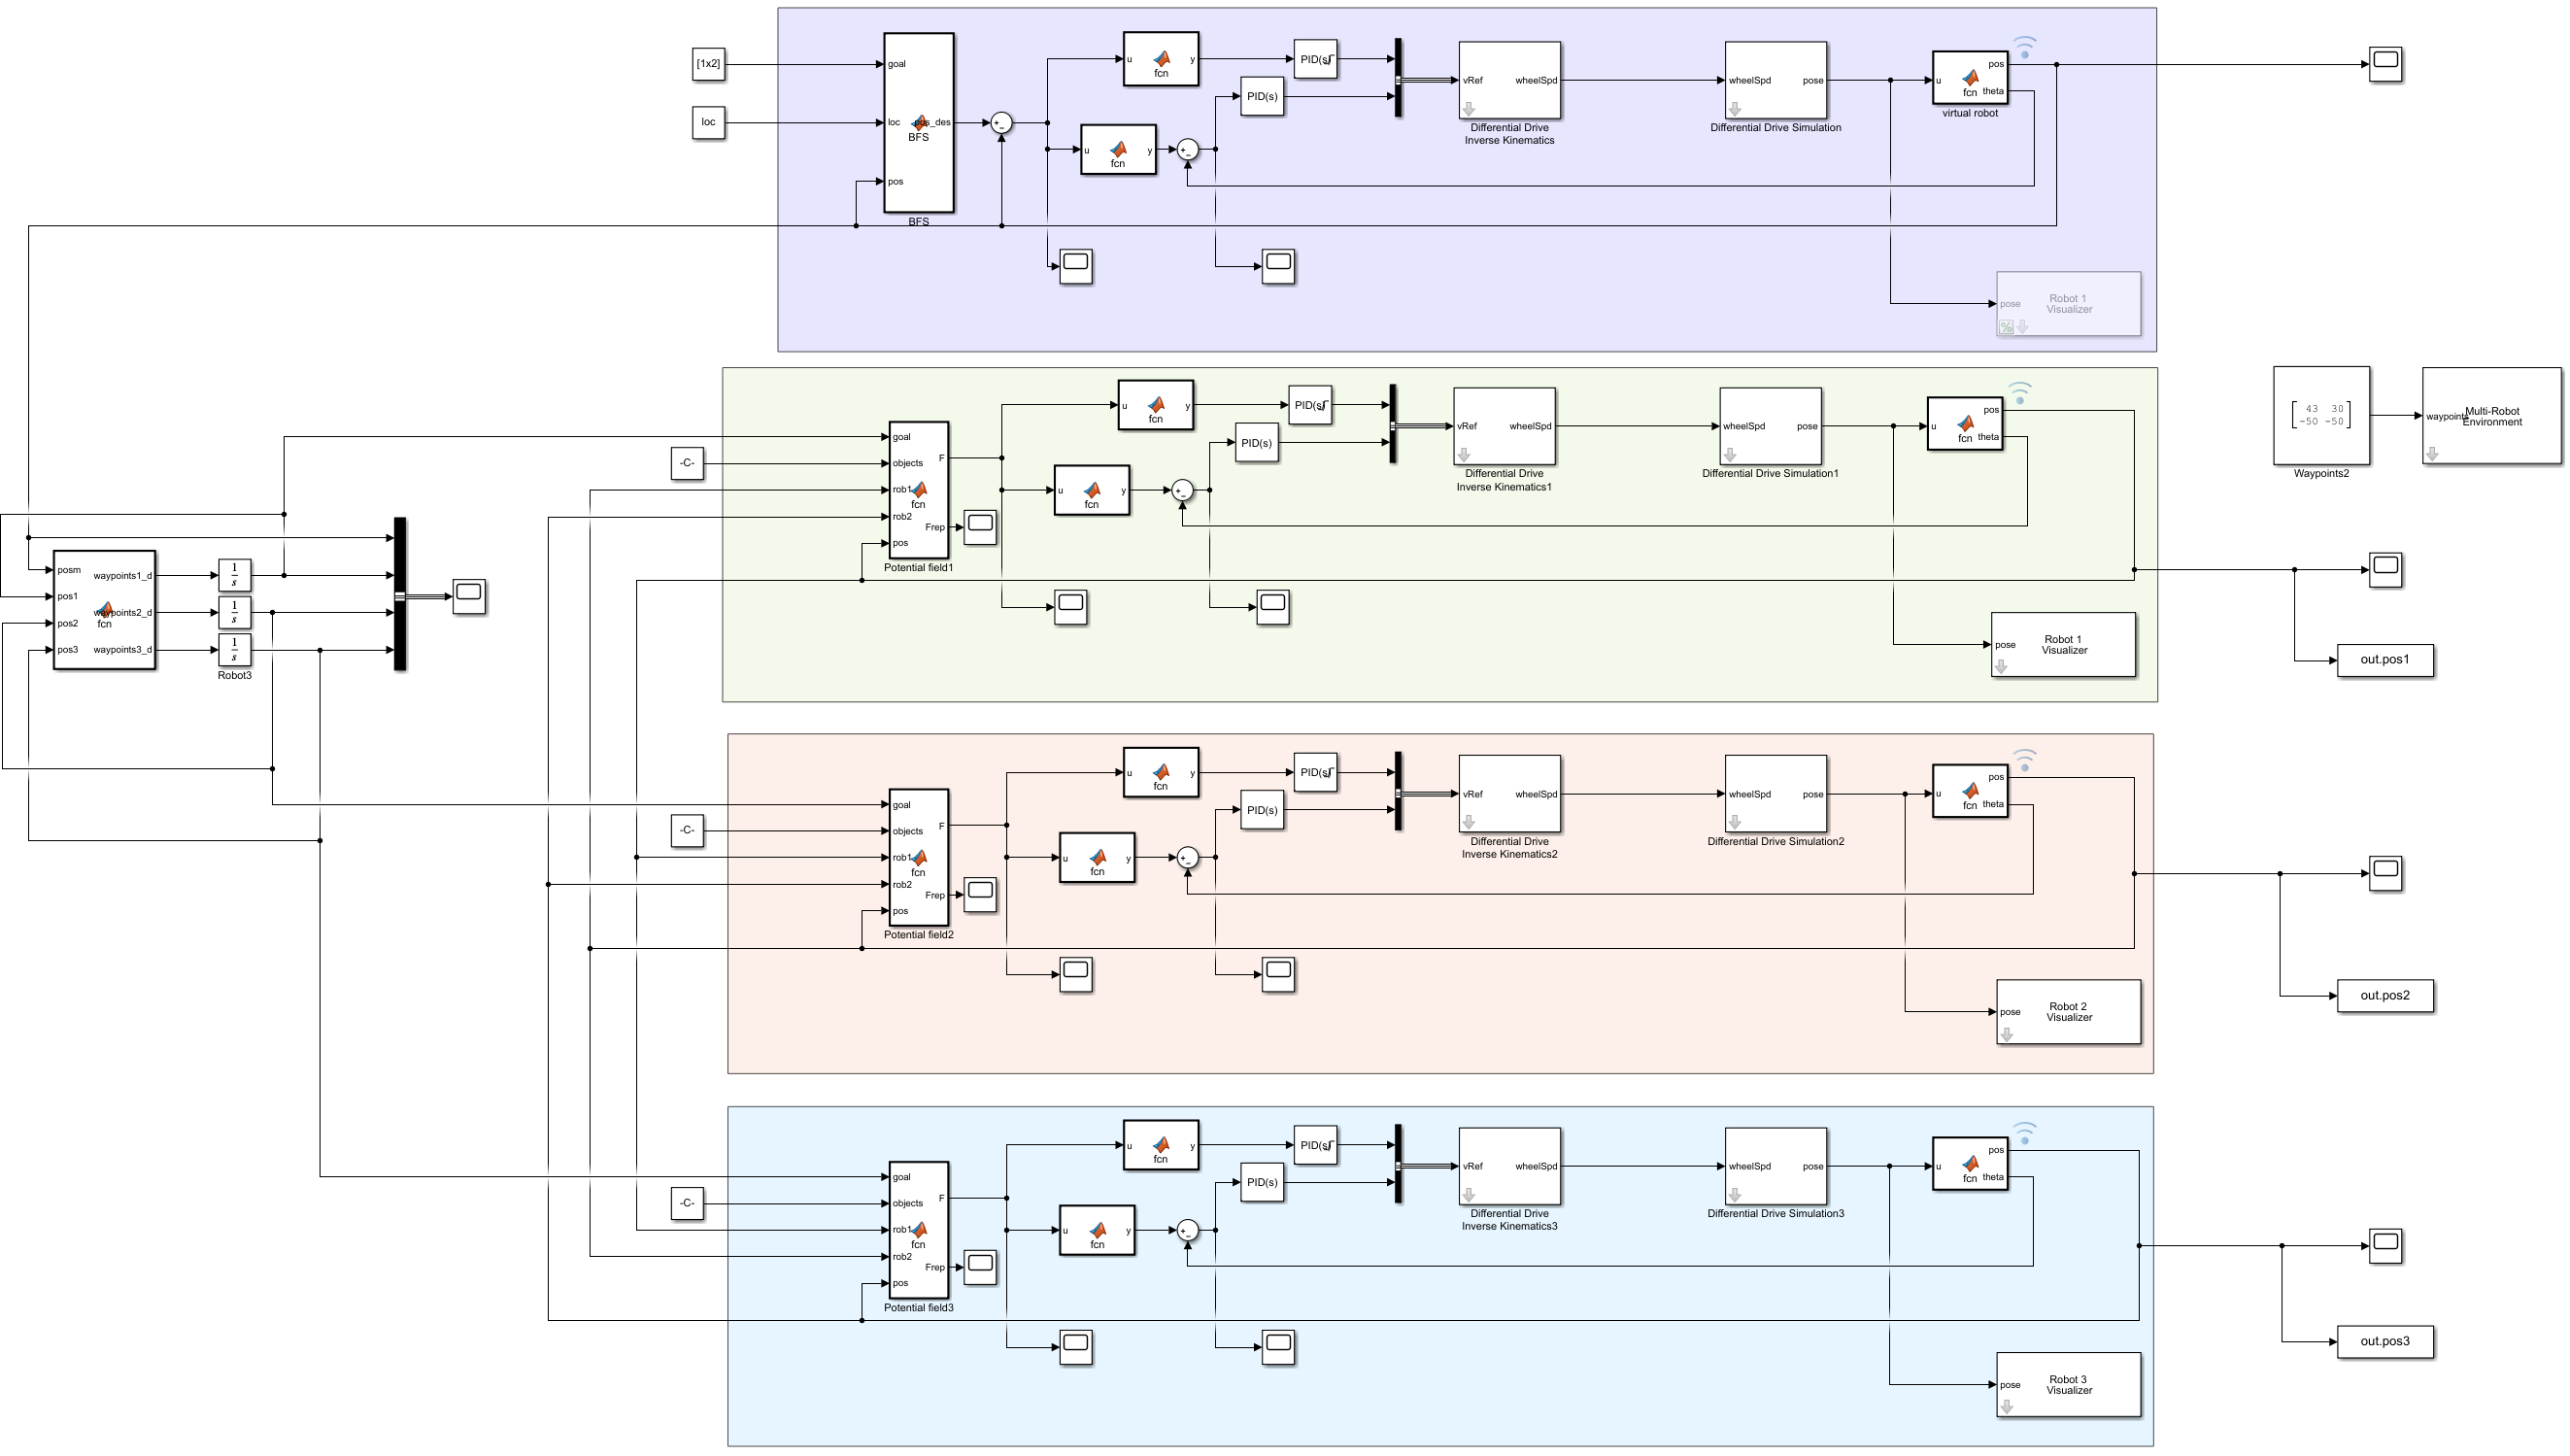
\includegraphics[scale=0.22]{Images/platoon-BFS-simulink.png}
	\caption{بلوک‌های شبیه‌سازی در روش \lr{BFS}}\label{Fig platoon-BSF-simulink}
\end{figure}

\begin{figure}[!h]
	\centering
	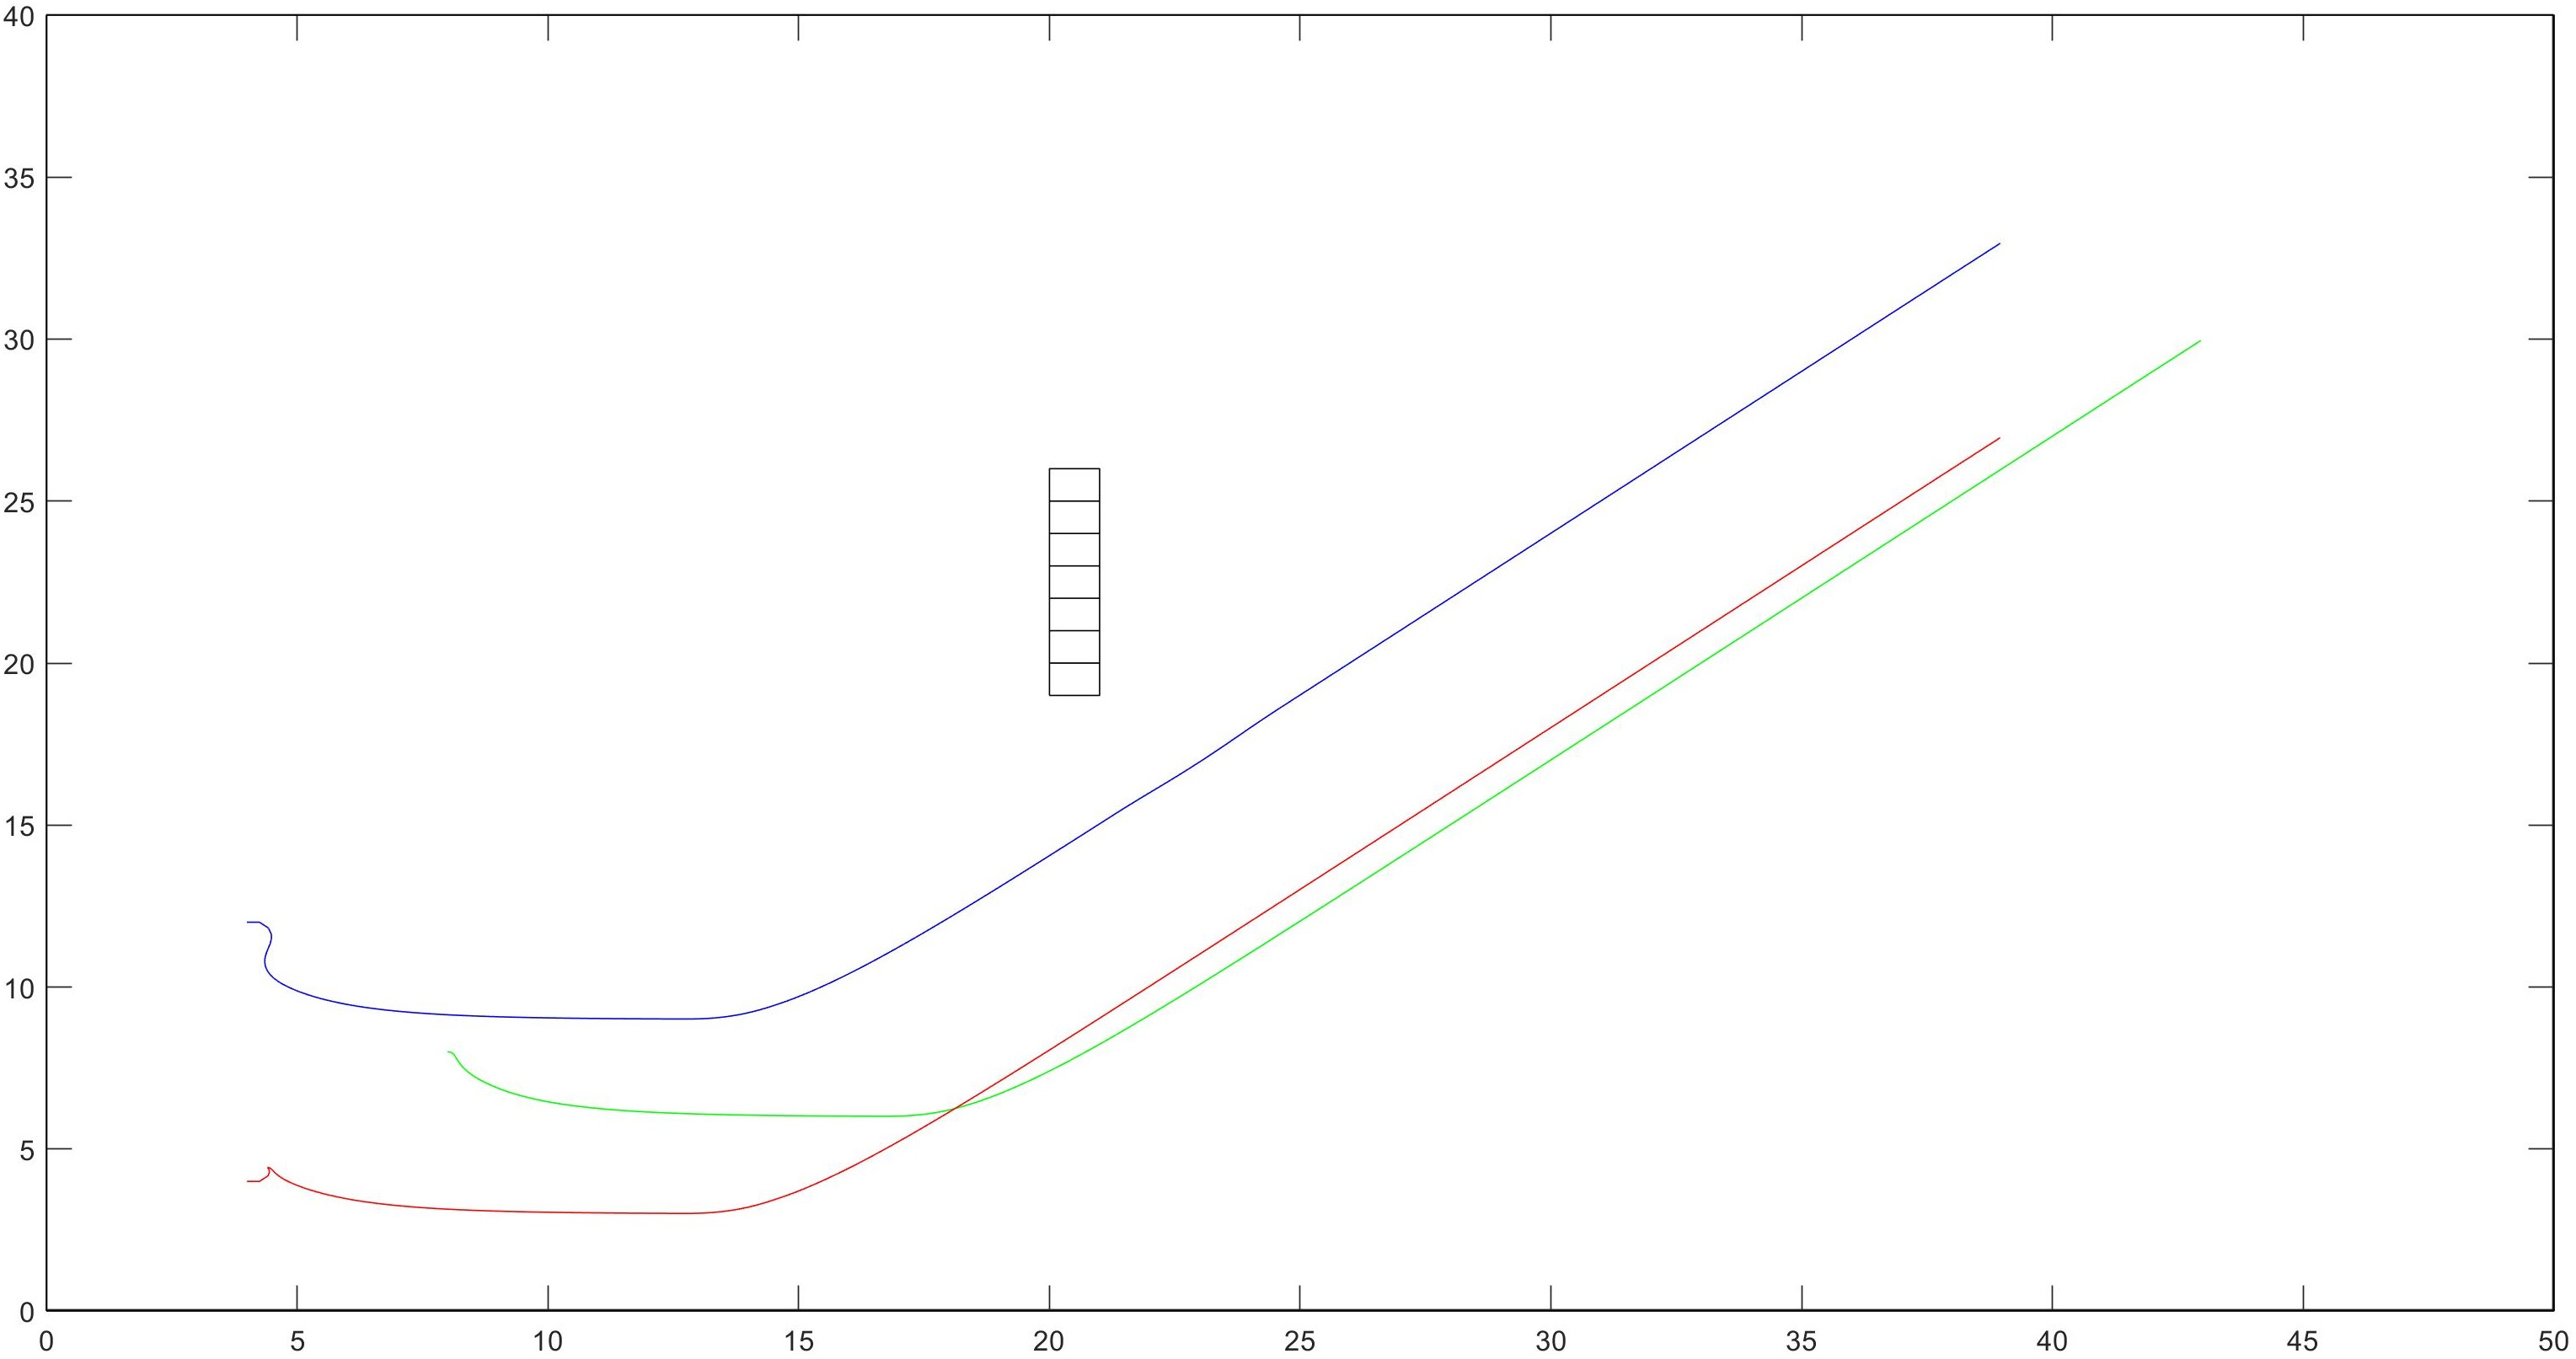
\includegraphics[scale=0.2]{Images/platoon-BFS-pos.jpg}
	\caption{مکان ربات‌ها در روش \lr{BFS}}\label{Fig platoon-BSF-pos}
\end{figure}

\newpage
\subsection{\lr{Greedy best-first search}}
پیاده‌سازی روش \lr{Greedy best-first search} برای مسیریابی اجماع ربات‌ها همراه با نتیجه‌ آن، به ترتیب در شکل‌های \ref{Fig platoon-Greedy-simulink} و \ref{Fig platoon-Greedy-pos} آمده است.
\begin{figure}[!h]
	\centering
	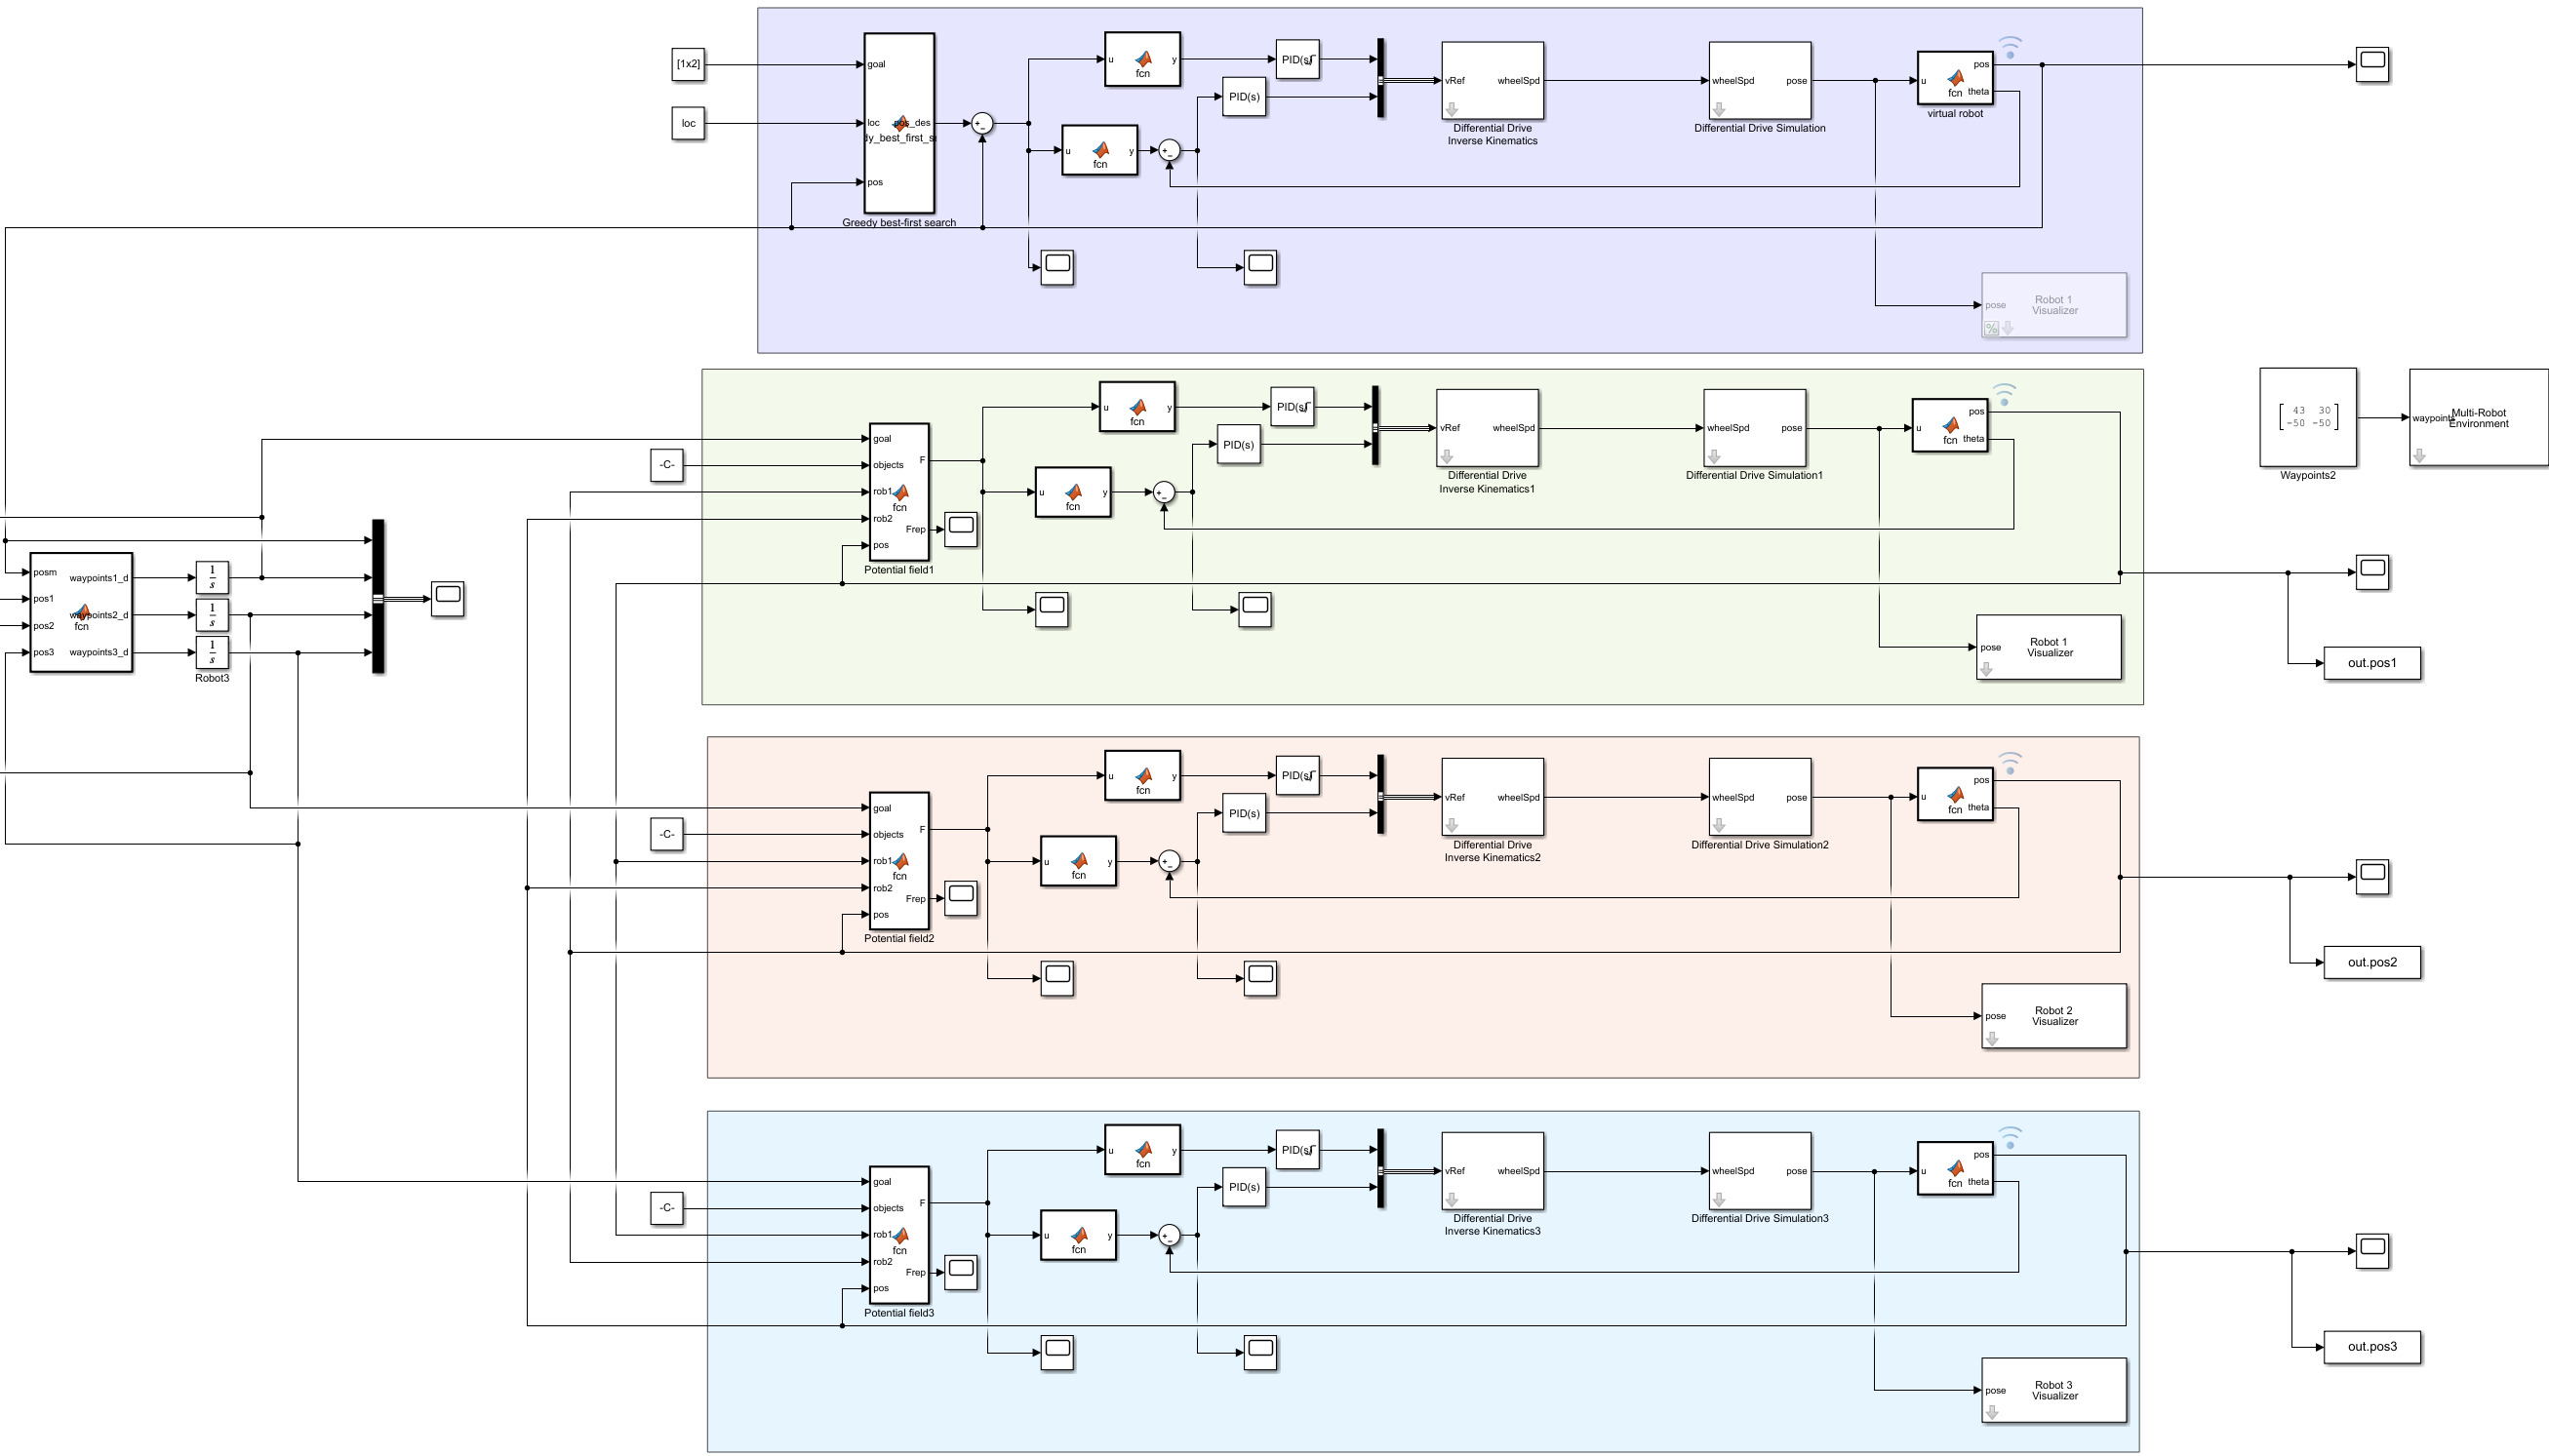
\includegraphics[scale=0.22]{Images/platoon-Greedy-simulink.png}
	\caption{بلوک‌های شبیه‌سازی در روش \lr{Greedy best-first search}}\label{Fig platoon-Greedy-simulink}
\end{figure}

\begin{figure}[!h]
	\centering
	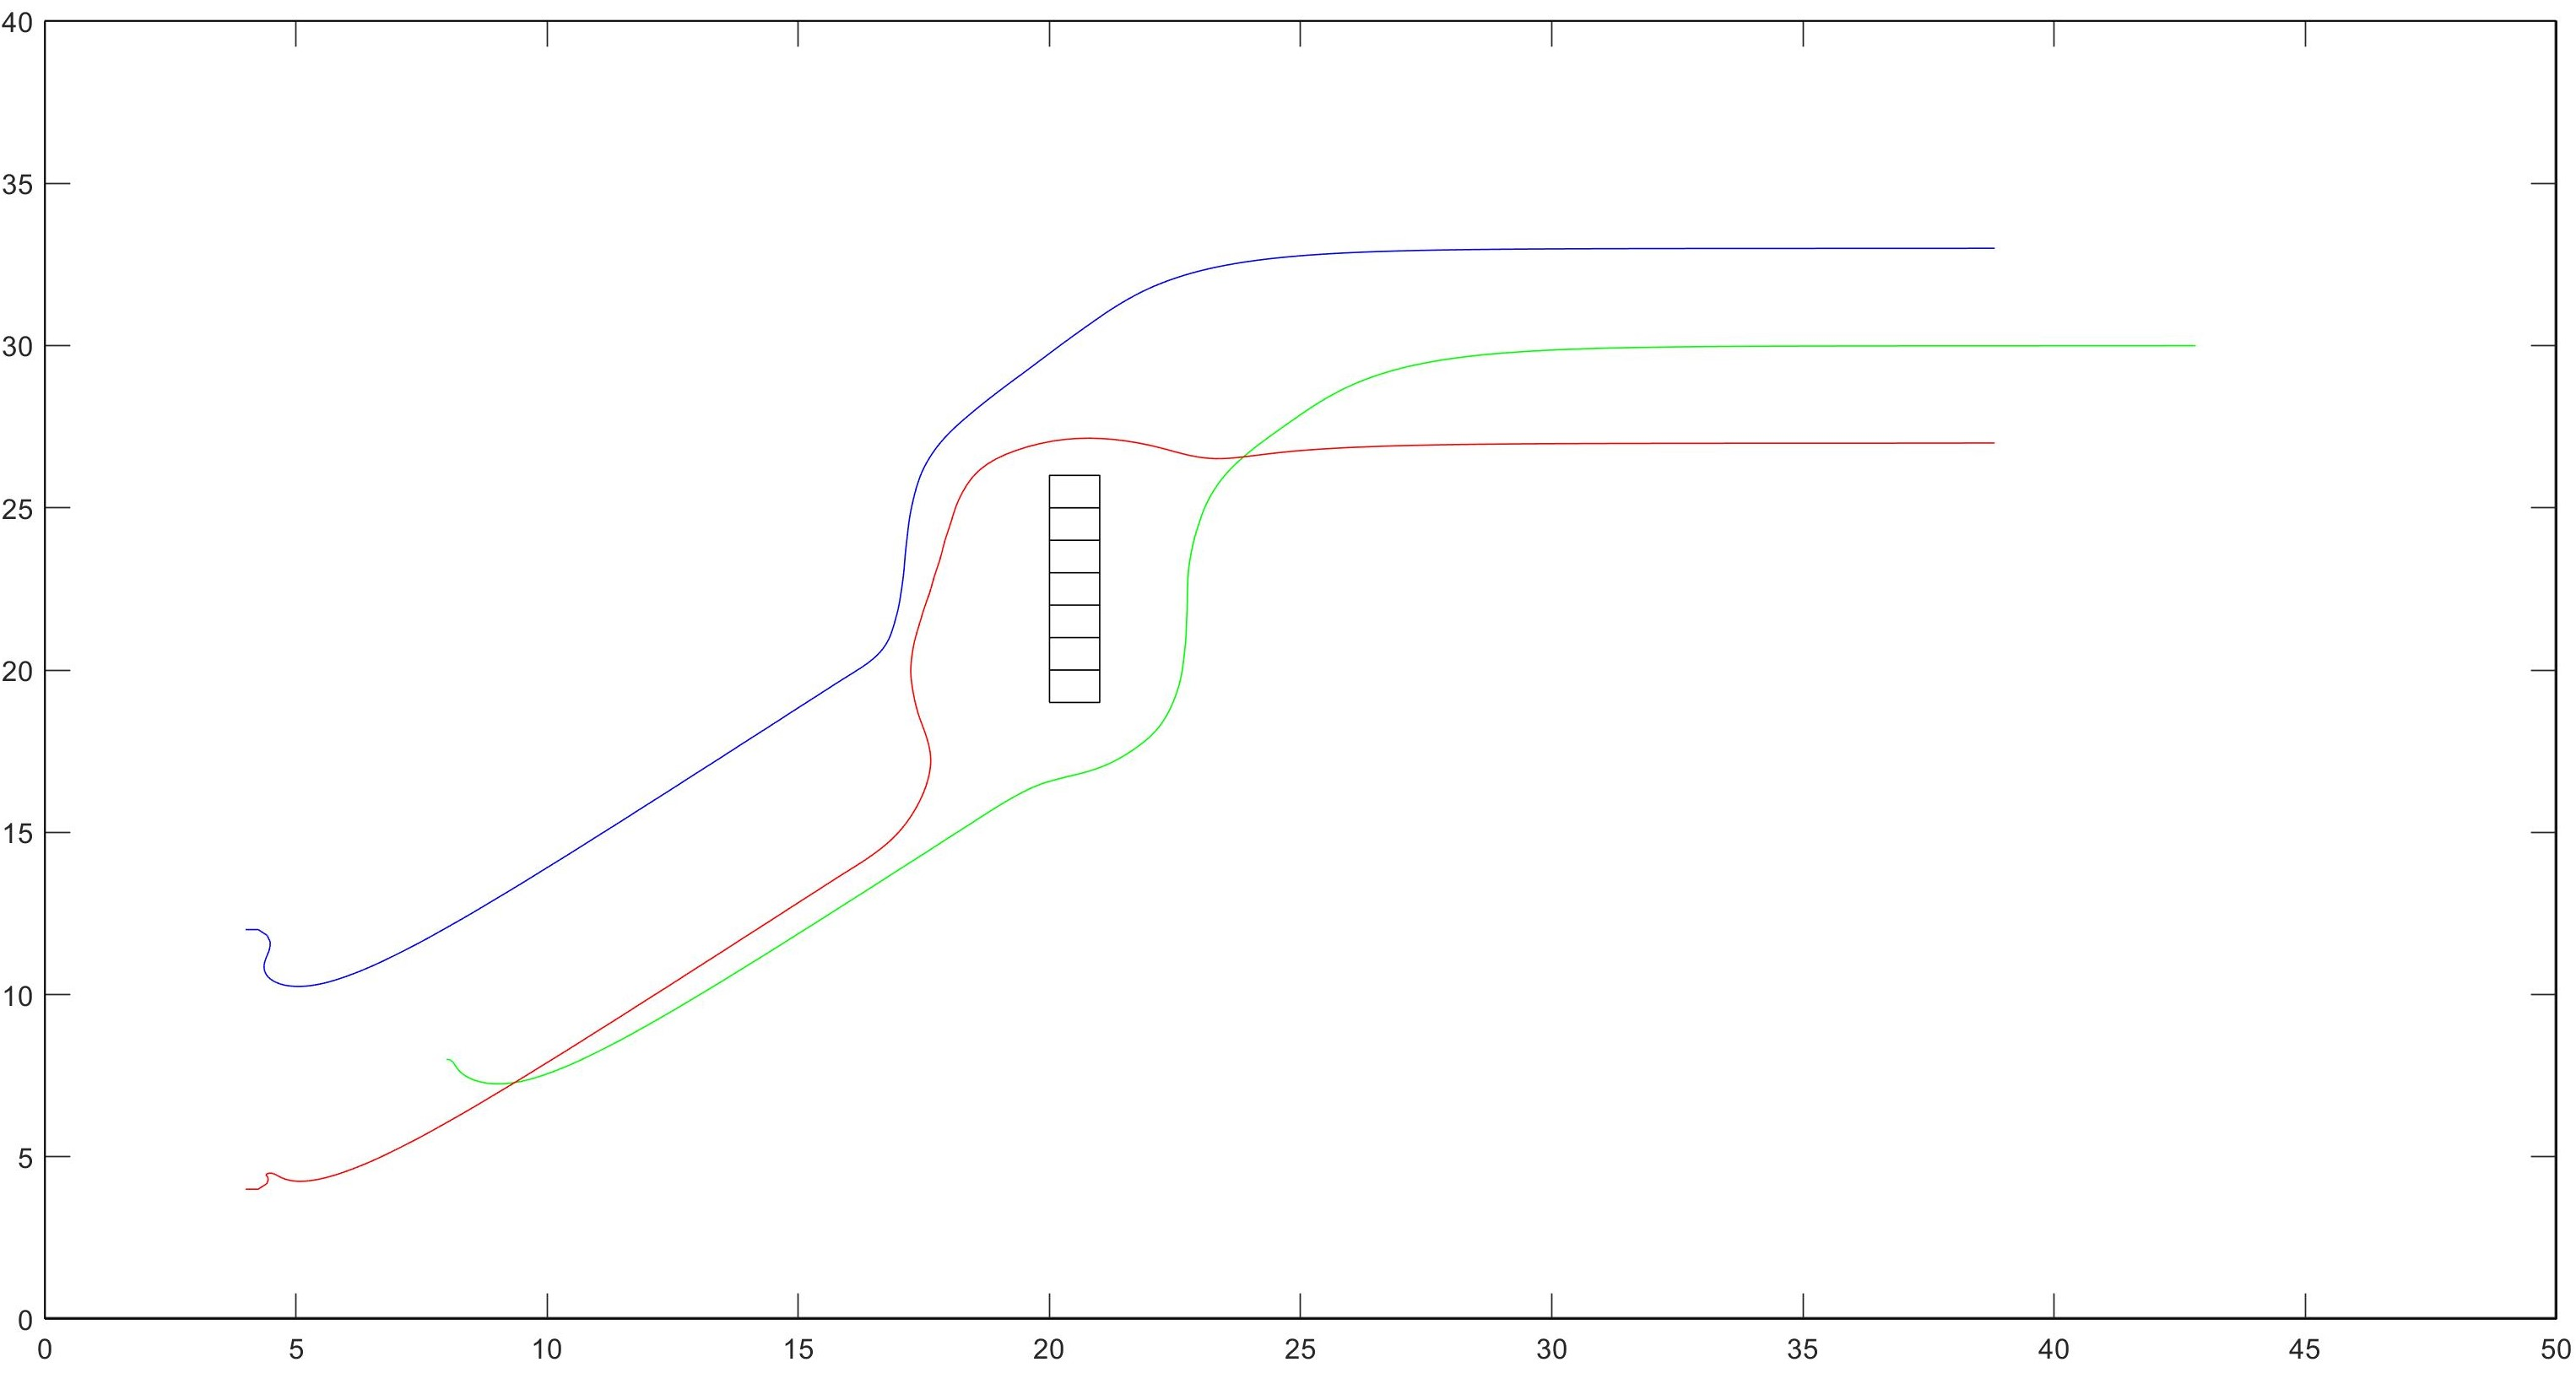
\includegraphics[scale=0.2]{Images/platoon-Greedy-pos.jpg}
	\caption{مکان ربات‌ها در روش \lr{Greedy best-first search}}\label{Fig platoon-Greedy-pos}
\end{figure}


\subsection{$A^*$}
روش $A^*$ برای مسیریابی اجماع ربات‌ها در شکل \ref{Fig platoon-A-star-simulink} پیاده‌سازی شده است. مسیر پیموده شده توسط هر ربات، در شکل \ref{Fig platoon-A-star-pos} قابل مشاهده می‌باشد.
\begin{figure}[!h]
	\centering
	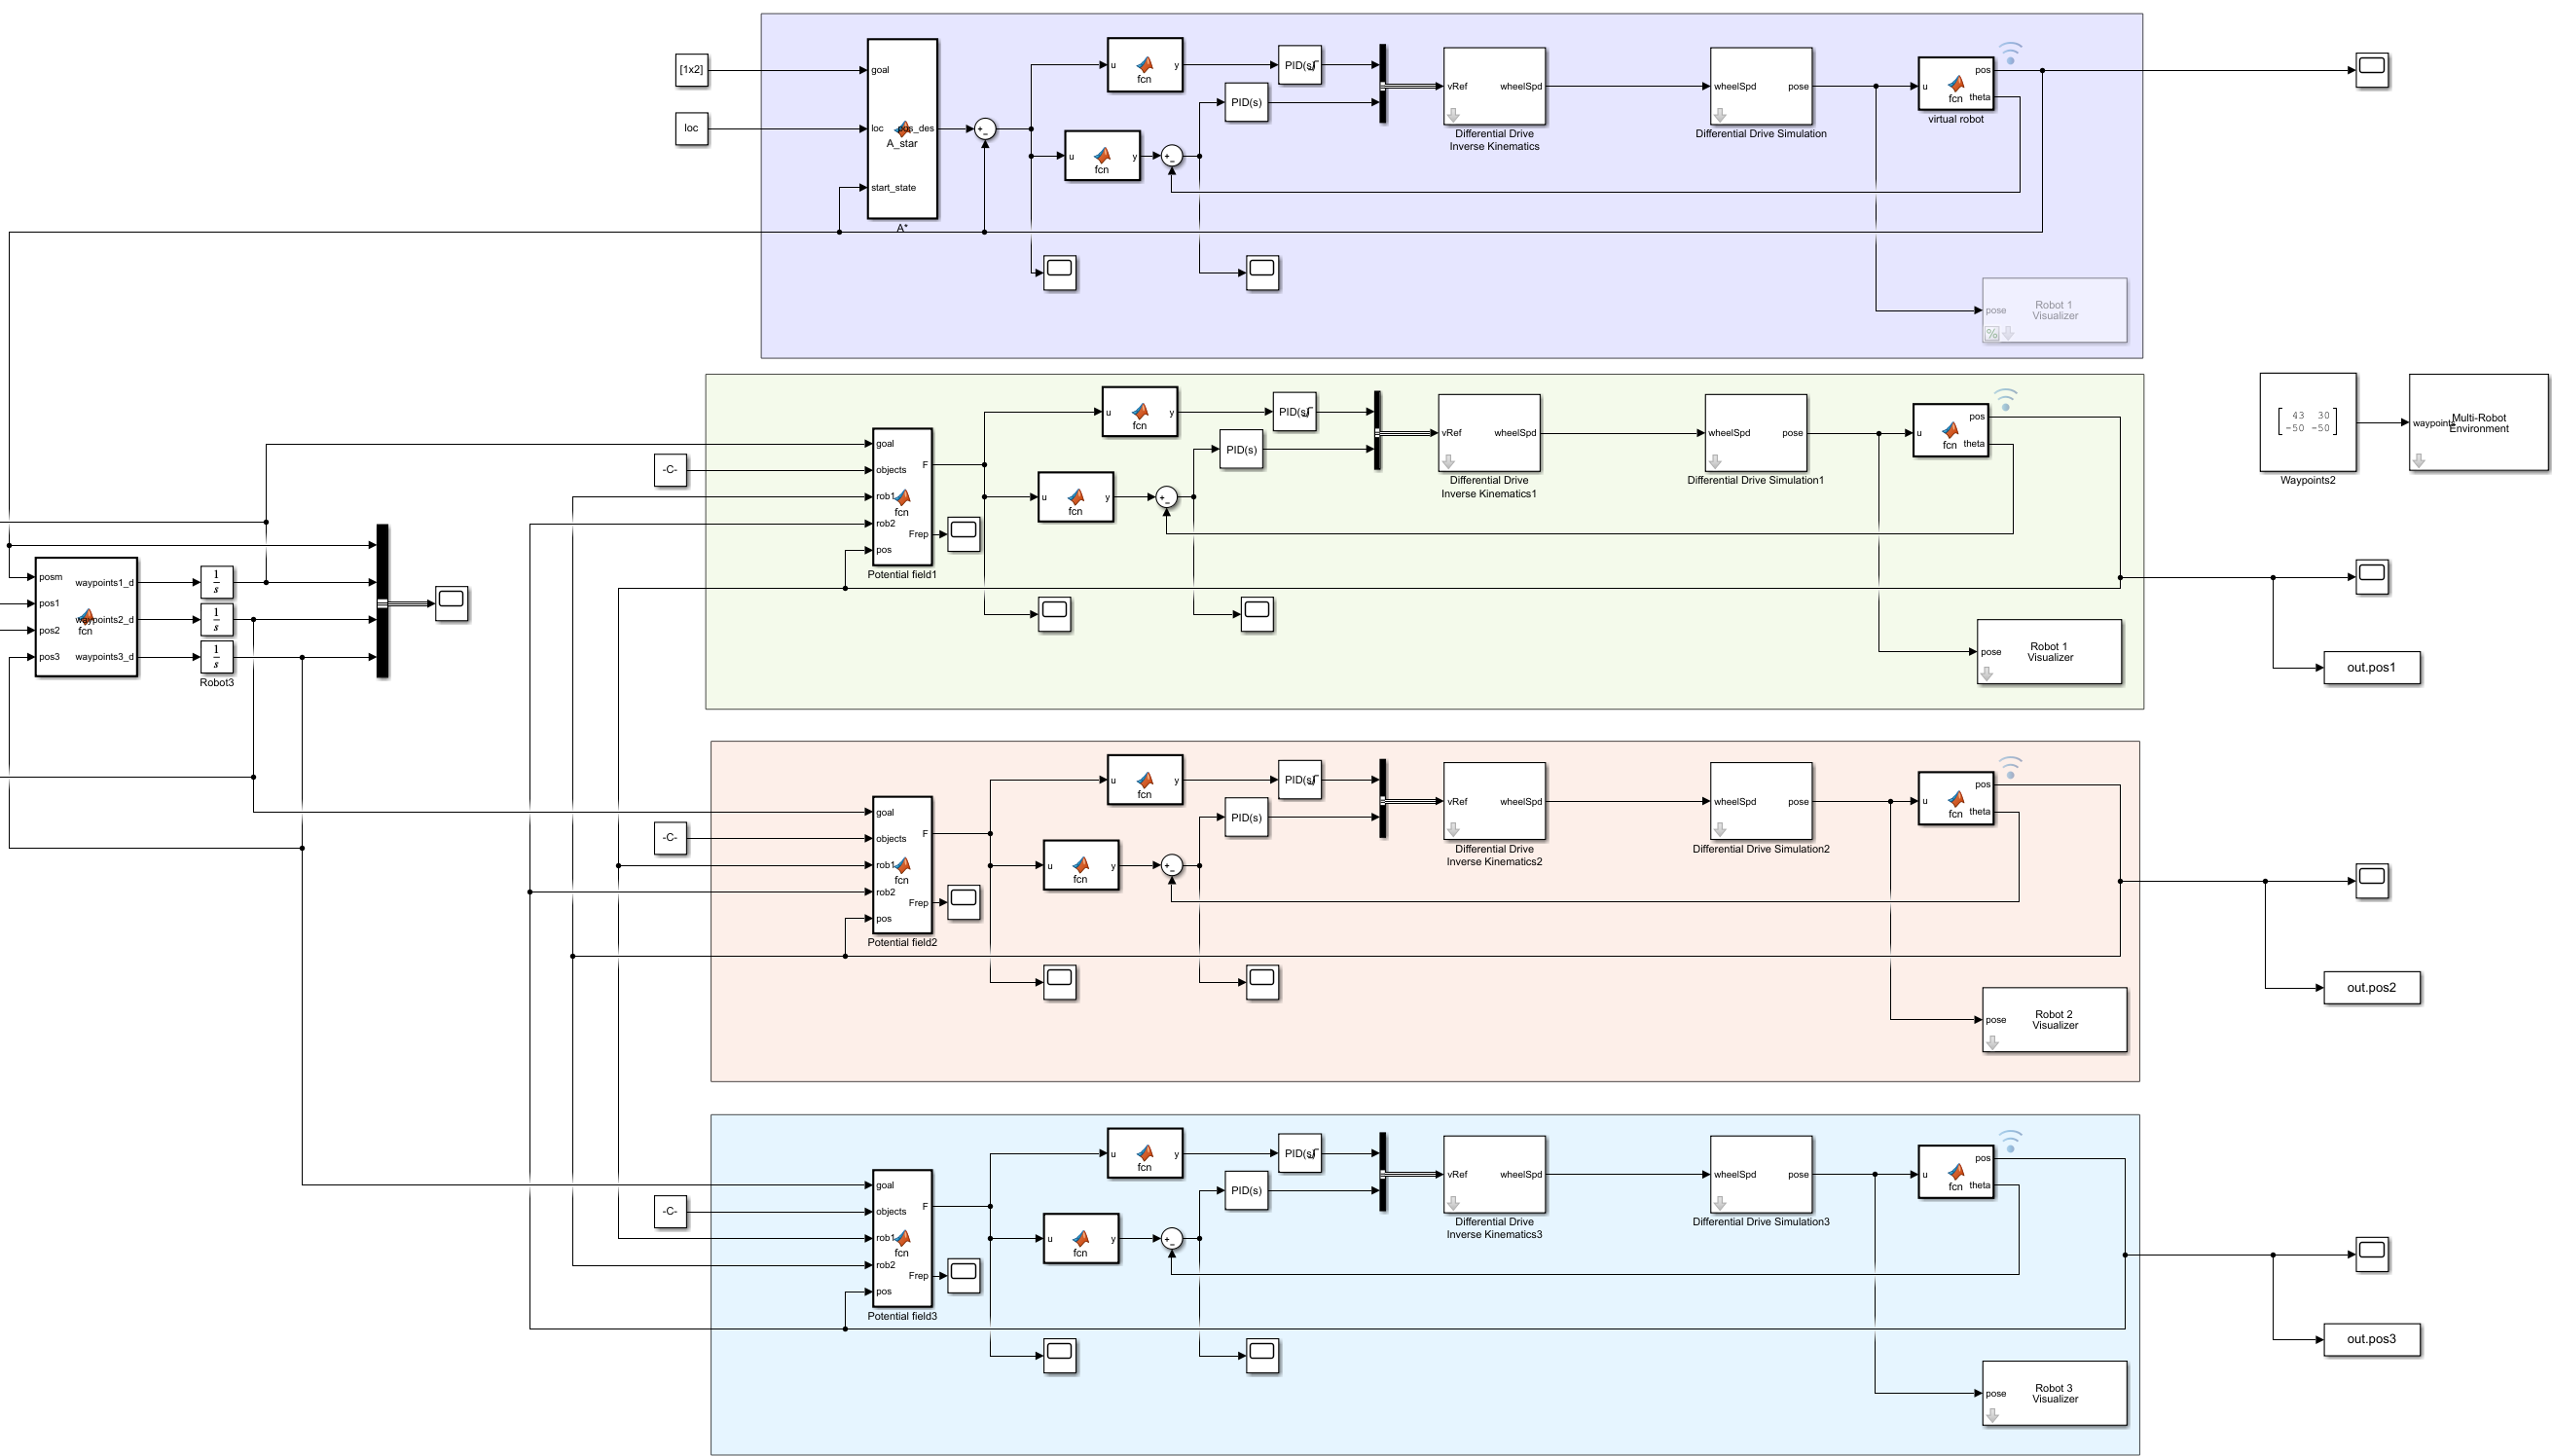
\includegraphics[scale=0.22]{Images/platoon-A-star-simulink.png}
	\caption{بلوک‌های شبیه‌سازی در روش $A^*$}\label{Fig platoon-A-star-simulink}
\end{figure}

\begin{figure}[!h]
	\centering
	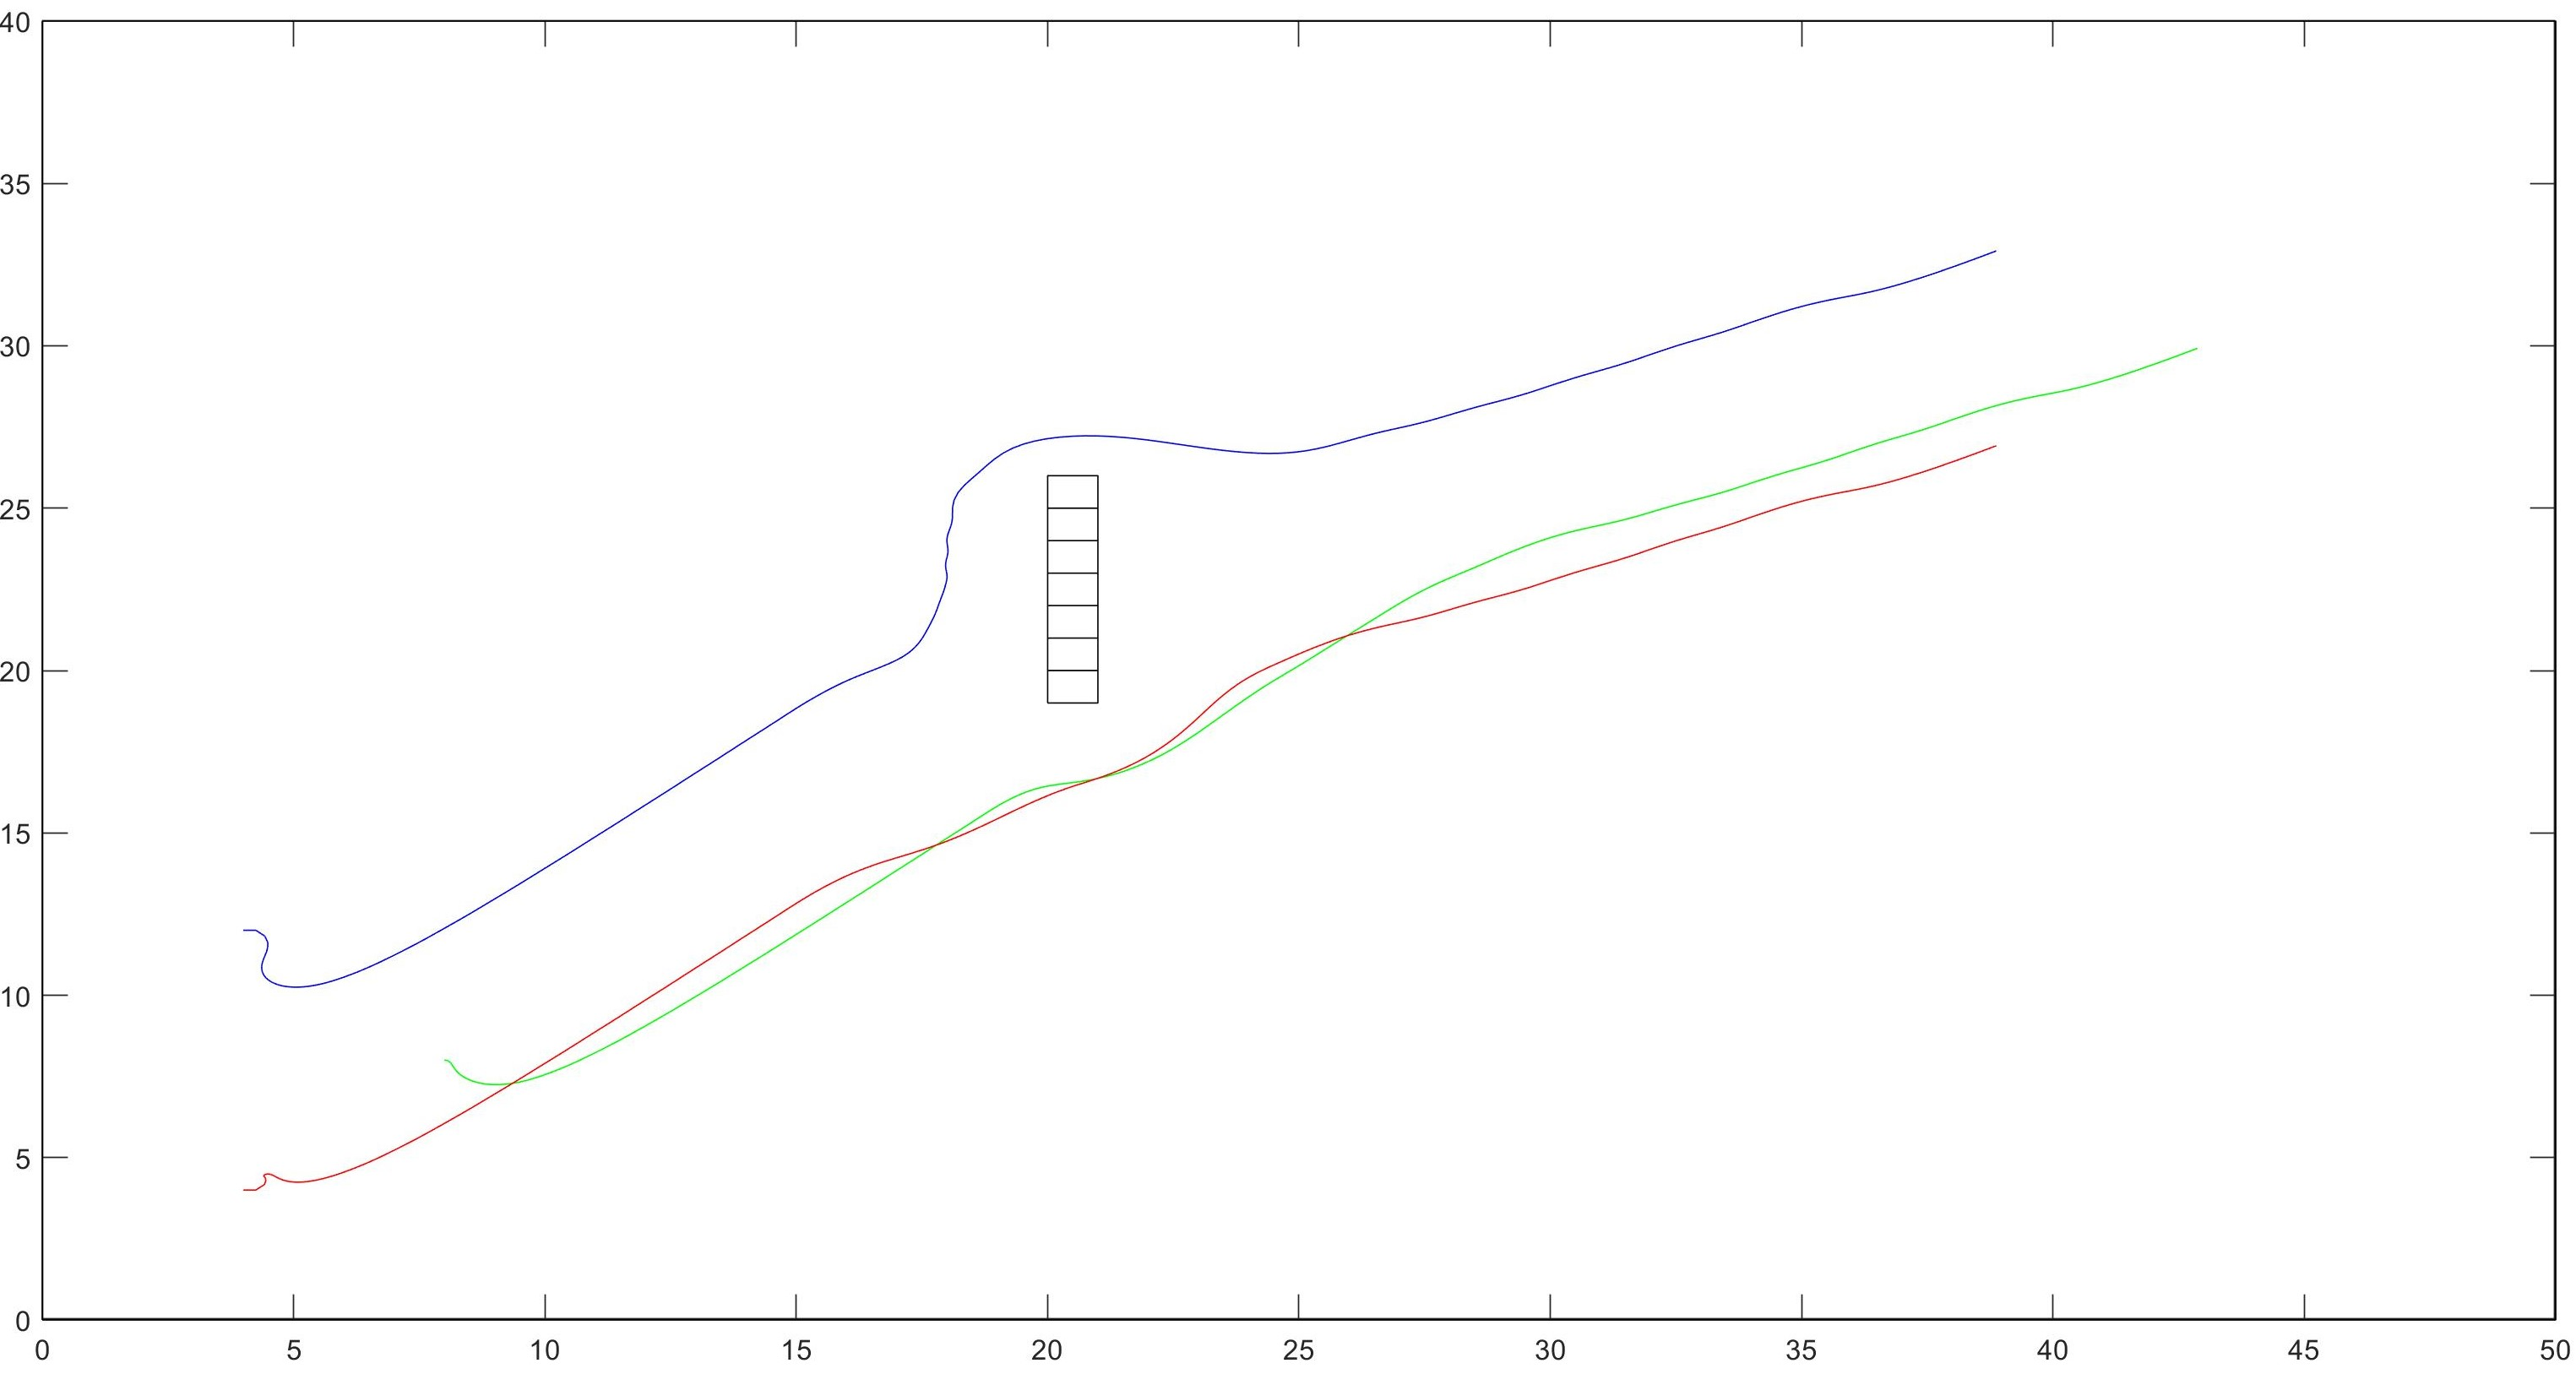
\includegraphics[scale=0.2]{Images/platoon-A-star-pos.jpg}
	\caption{مکان ربات‌ها در روش $A^*$}\label{Fig platoon-A-star-pos}
\end{figure}

\section{\lr{Q-learning}}
در این قسمت نتایج الگوریتم \lr{Q-learning} بررسی خواهد شد. قابل ذکر است که مقادیر یادگیری به شرح زیر هستند:
\begin{itemize}
	\item $\alpha$ = 0/9
	\item $\gamma$ = 0/9
	\item بیشترین تعداد گام‌ها = 100
	\item حد بیشترین اختلاف در تابع \lr{V} = 0/0001
	\item $R=-\|a\|_2$
\end{itemize}

بلوک‌های شبیه‌سازی همانند شکل \ref{Fig platoon-QL} بسته شده‌اند. همچنین مسیر پیموده شده توسط هر ربات در شکل \ref{Fig platoon-QL-pos} نشان داده شده است. در پیاده‌سازی آنلاین، مقادیر \lr{V} و \lr{Q} نگه‌داری می‌شوند و در هر دوره محاسباتی تنها به روزرسانی می‌گردند. لذا همانطور که مشخص است در یکی دو سیاست اولیه اخذ شده، هنوز به بهینگی نرسیده‌ایم اما پس از 2 انتخاب، سیاست‌ها بهینه هستند.
\begin{figure}[!h]
	\centering
	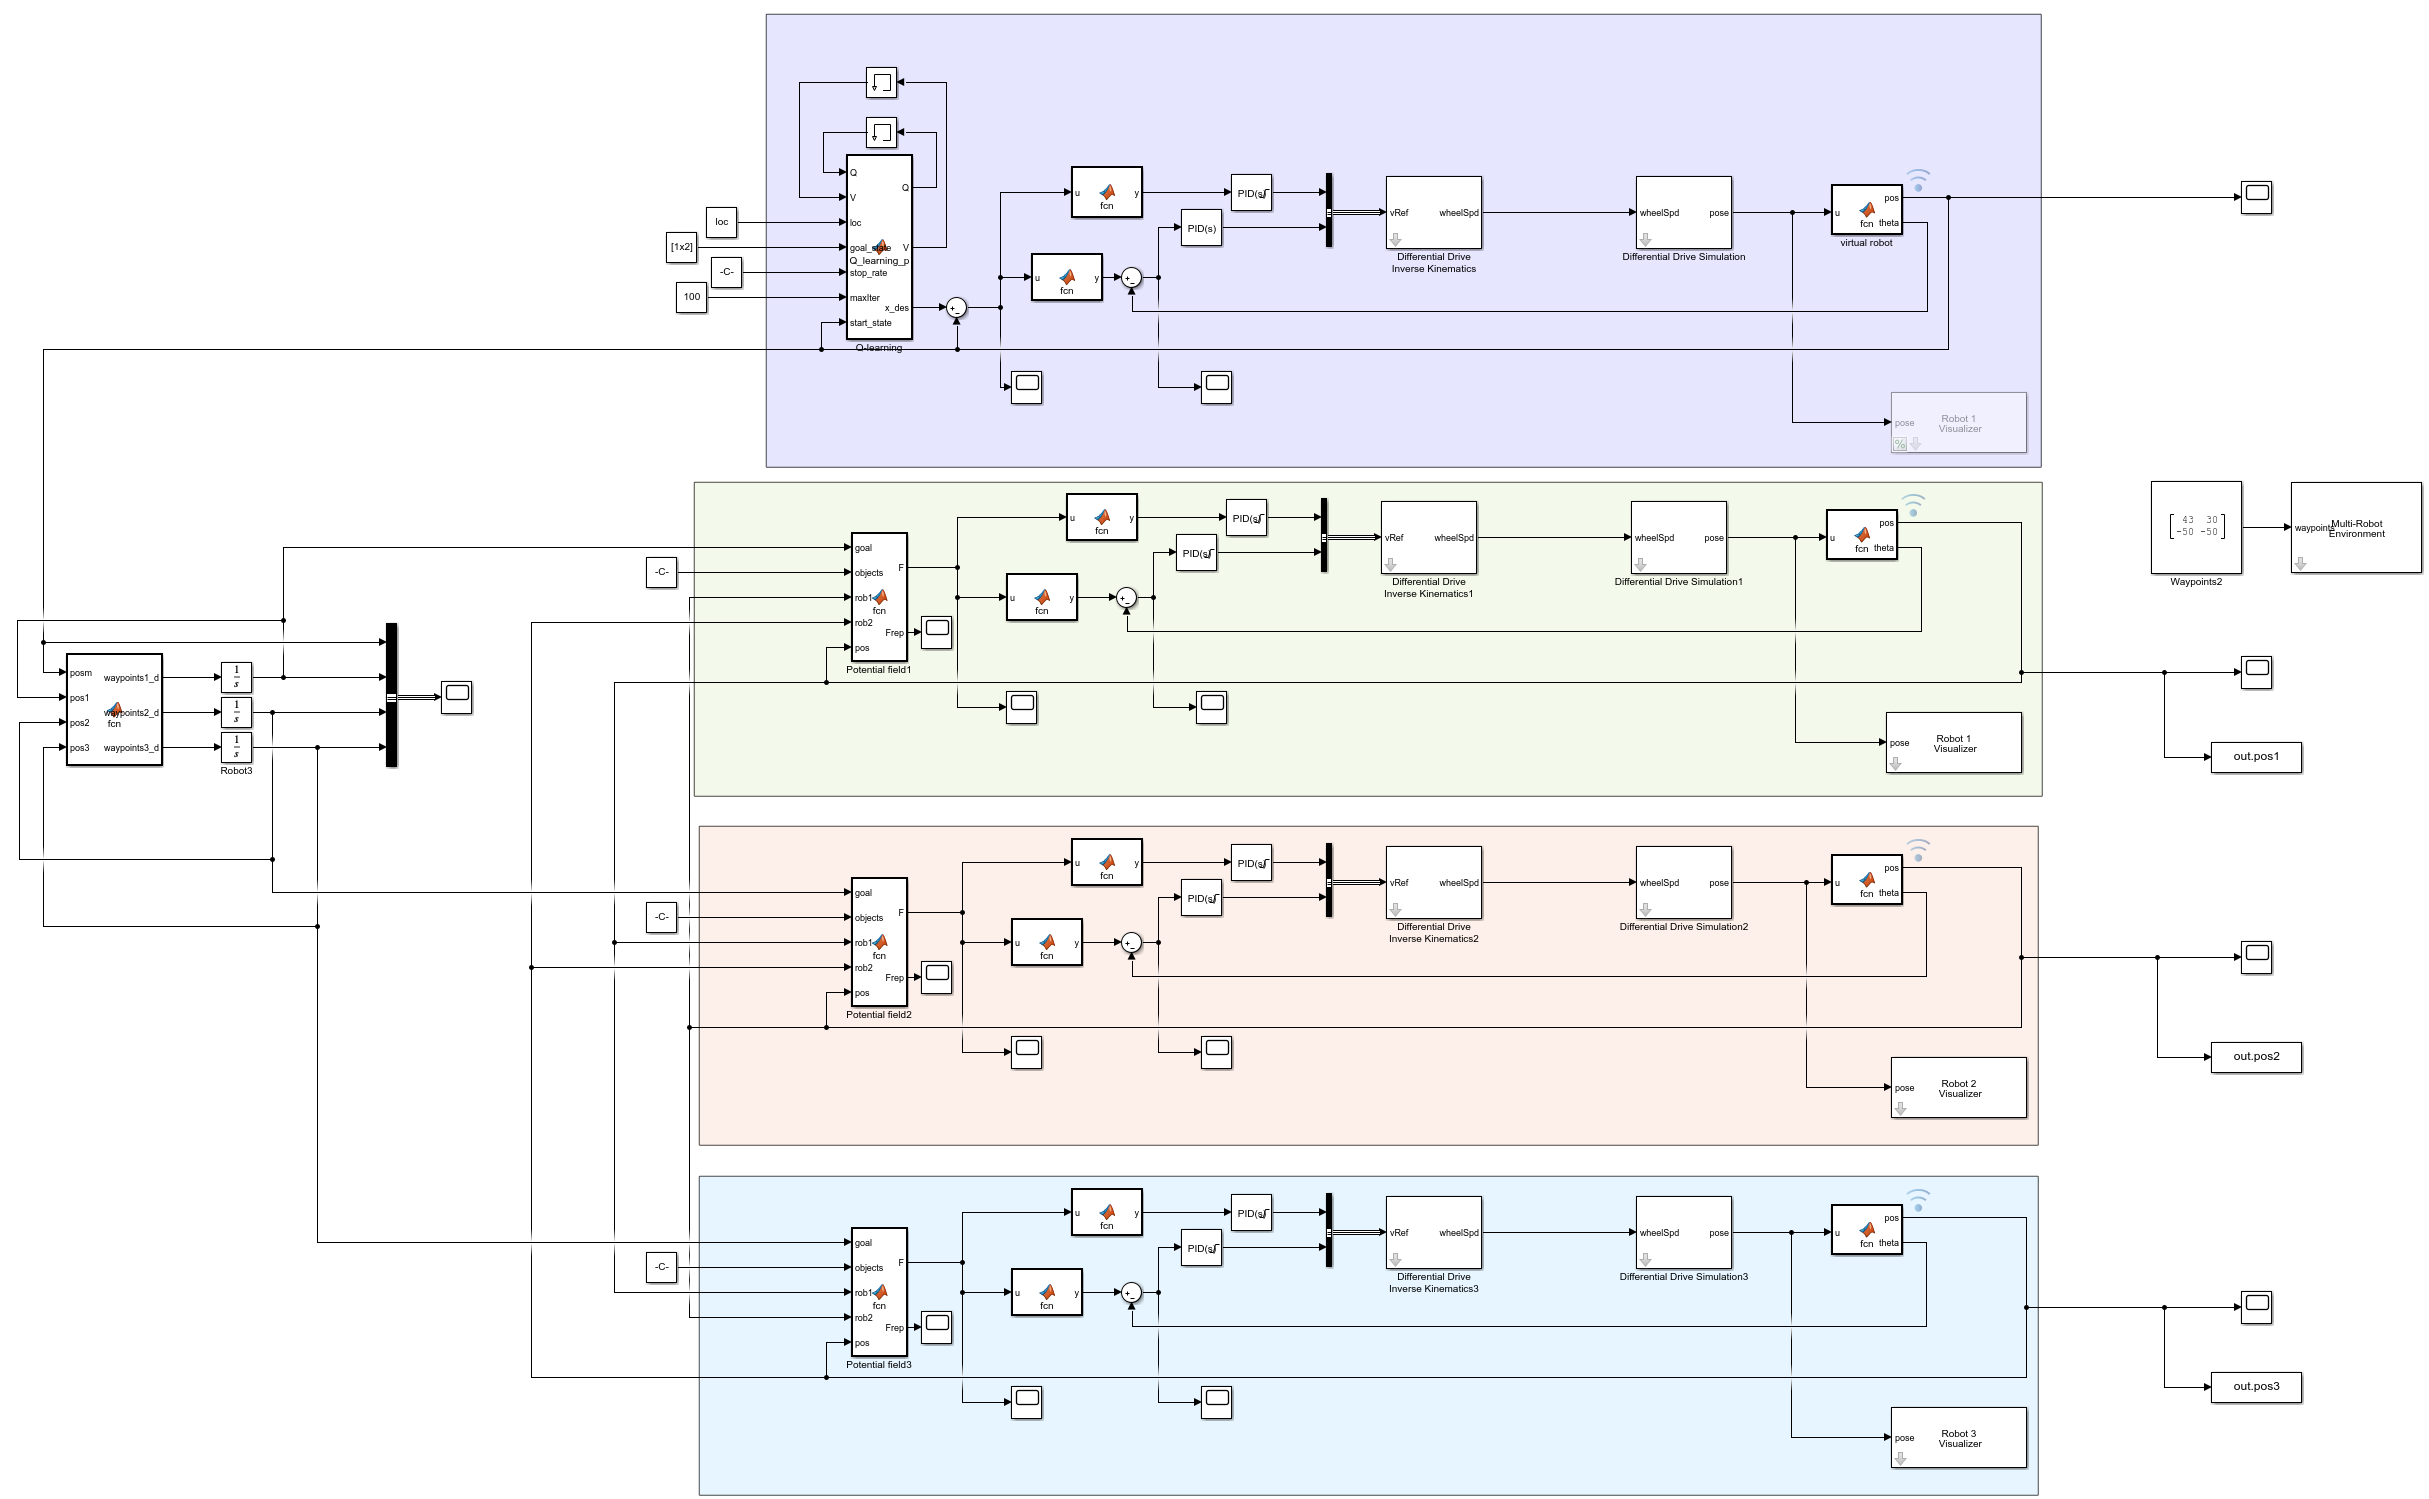
\includegraphics[scale=0.25]{Images/platoon-QL.png}
	\caption{بلوک‌های شبیه‌سازی در روش \lr{Q-learning}}\label{Fig platoon-QL}
\end{figure}

\begin{figure}[!h]
	\centering
	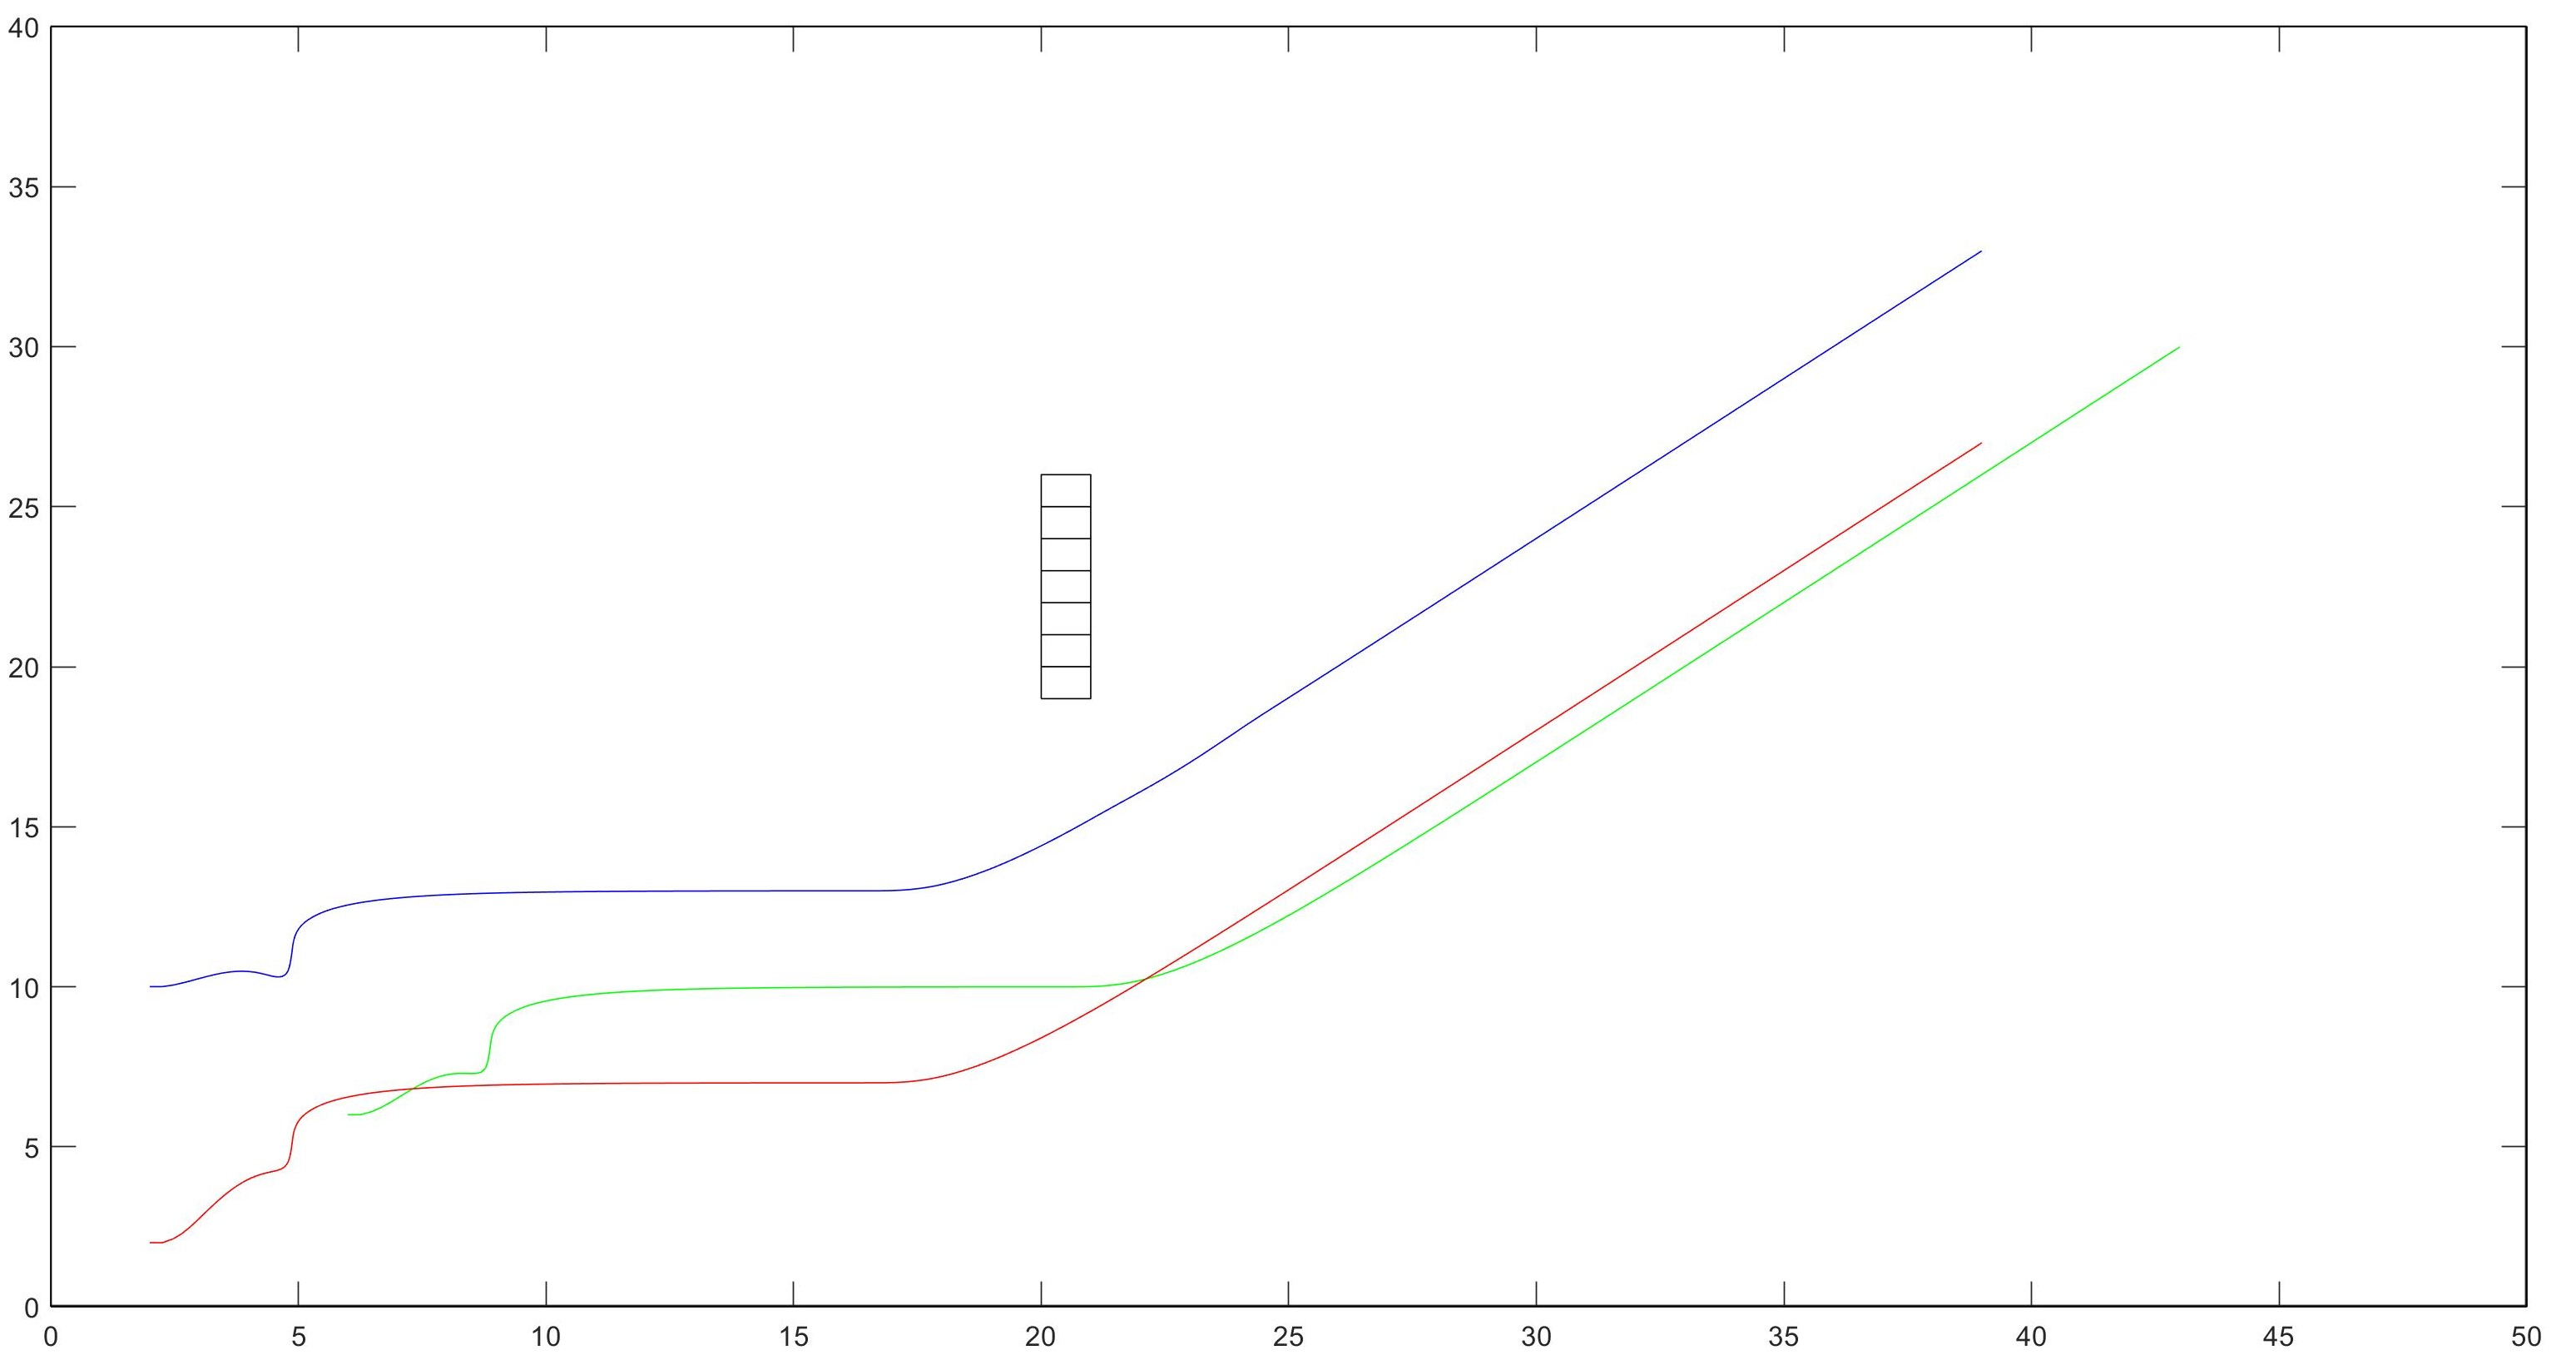
\includegraphics[scale=0.2]{Images/platoon-QL-pos.jpg}
	\caption{مکان ربات‌ها در روش \lr{Q-learning}}\label{Fig platoon-QL-pos}
\end{figure}

\newpage
\section{مسیریابی در حضور موانع متحرک}
در ادامه نتایج گرفته شده در برابر موانع متحرک برای الگوریتم‌های بالا به نمایش در آمده‌اند. قابل ذکر است که فیلم پاسخ‌های گرفته شده در \cite{roozbeh2020} موجود می‌باشد. روش مواجهه به موانع متحرک به این صورت بوده است که جابه‌جایی آن‌ها در یک بازه زمانی محاسبه گردد و سپس طبق جابه‌جایی انجام شده در لحظه قبل و داشتن موقعیت لحظه حال، موقعیت مانع متحرک در لحظه بعدی تقریب زده شود. این روش بسیار ساده است و قابل ارتقا و دقیق‌تر شدن می‌باشد.
\begin{equation}
	X_{n+1} = X_n + (X_n - X_{n-1}) = 2X_n - X_{n-1}
\end{equation}

شبیه‌سازی برای \lr{Q-learning} در عکس \ref{Fig dynamic-QL} نشان داده شده است.
\begin{figure}[!h]
	\centering
	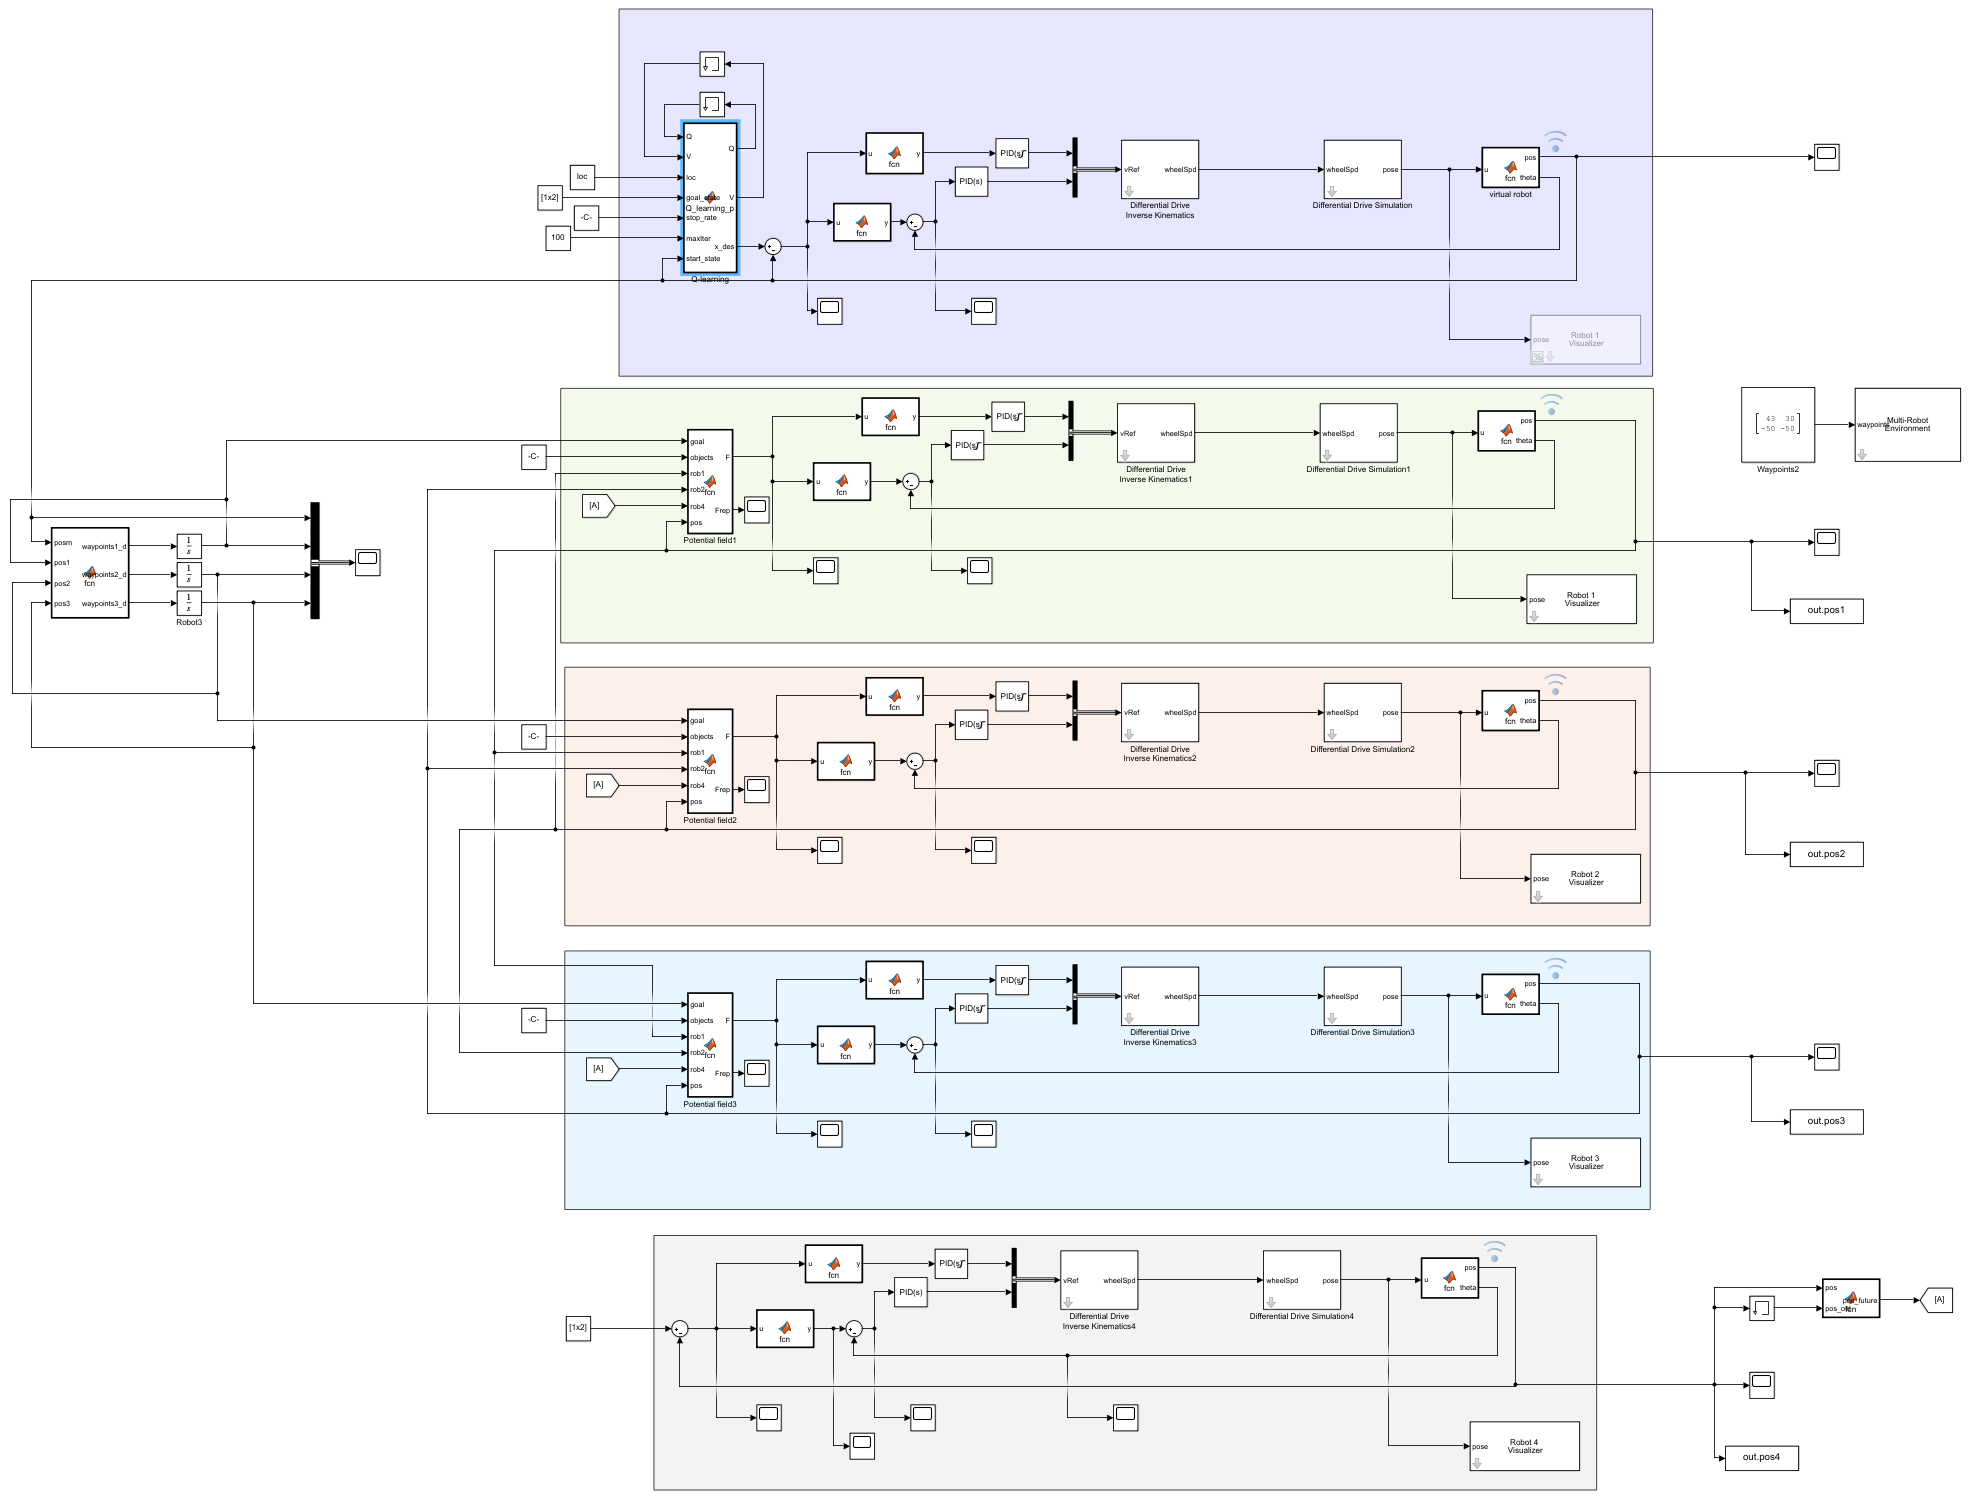
\includegraphics[scale=0.25]{Images/dynamic-QL.png}
	\caption{بلوک‌های شبیه‌سازی در روش \lr{Q-learning} همراه با مانع متحرک}\label{Fig dynamic-QL}
\end{figure}

نتایج برای هر الگوریتم نیز در عکس‌های زیر نشان داده شده‌اند. مسیرهای سبز، قرمز و آبی توسط ربات‌های پلتون و مسیر مشکی رنگ توسط مانع متحرک که خود نیز یک ربات است پیموده شده‌اند.
\begin{figure}[!h]
	\centering
	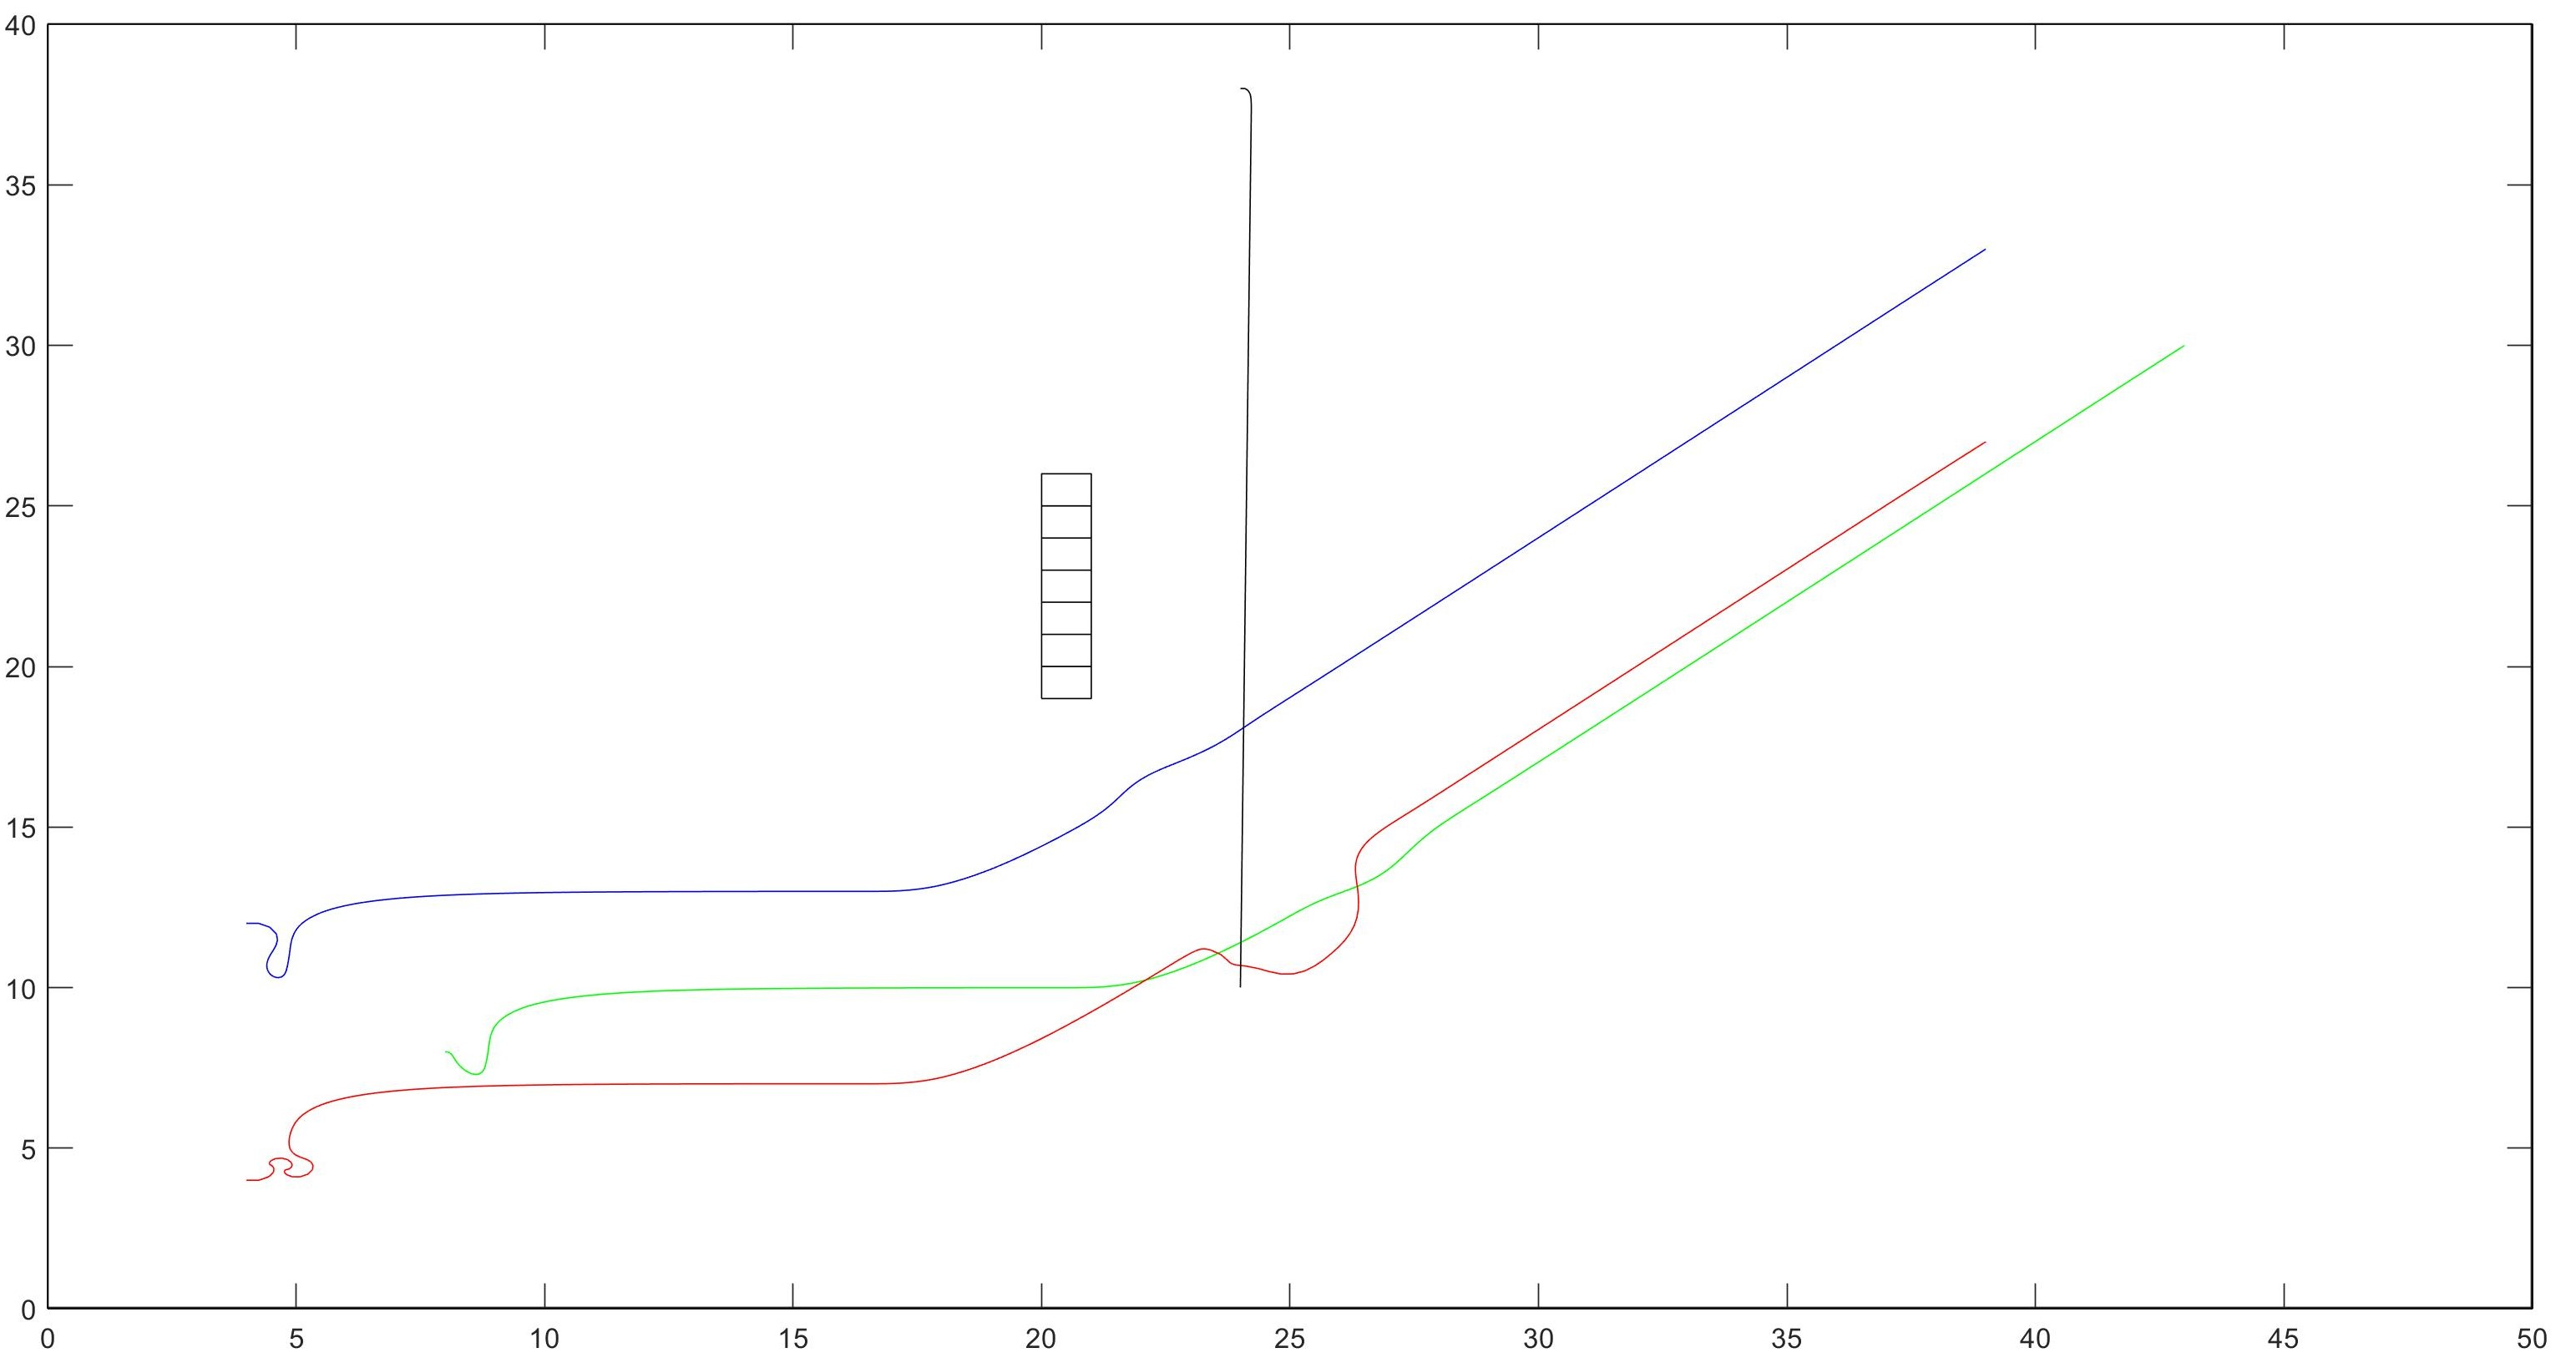
\includegraphics[scale=0.2]{Images/dynamic-QL.jpg}
	\caption{مکان ربات‌ها در روش \lr{Q-learning} همراه با مانع متحرک}
\end{figure}

\begin{figure}[!h]
	\centering
	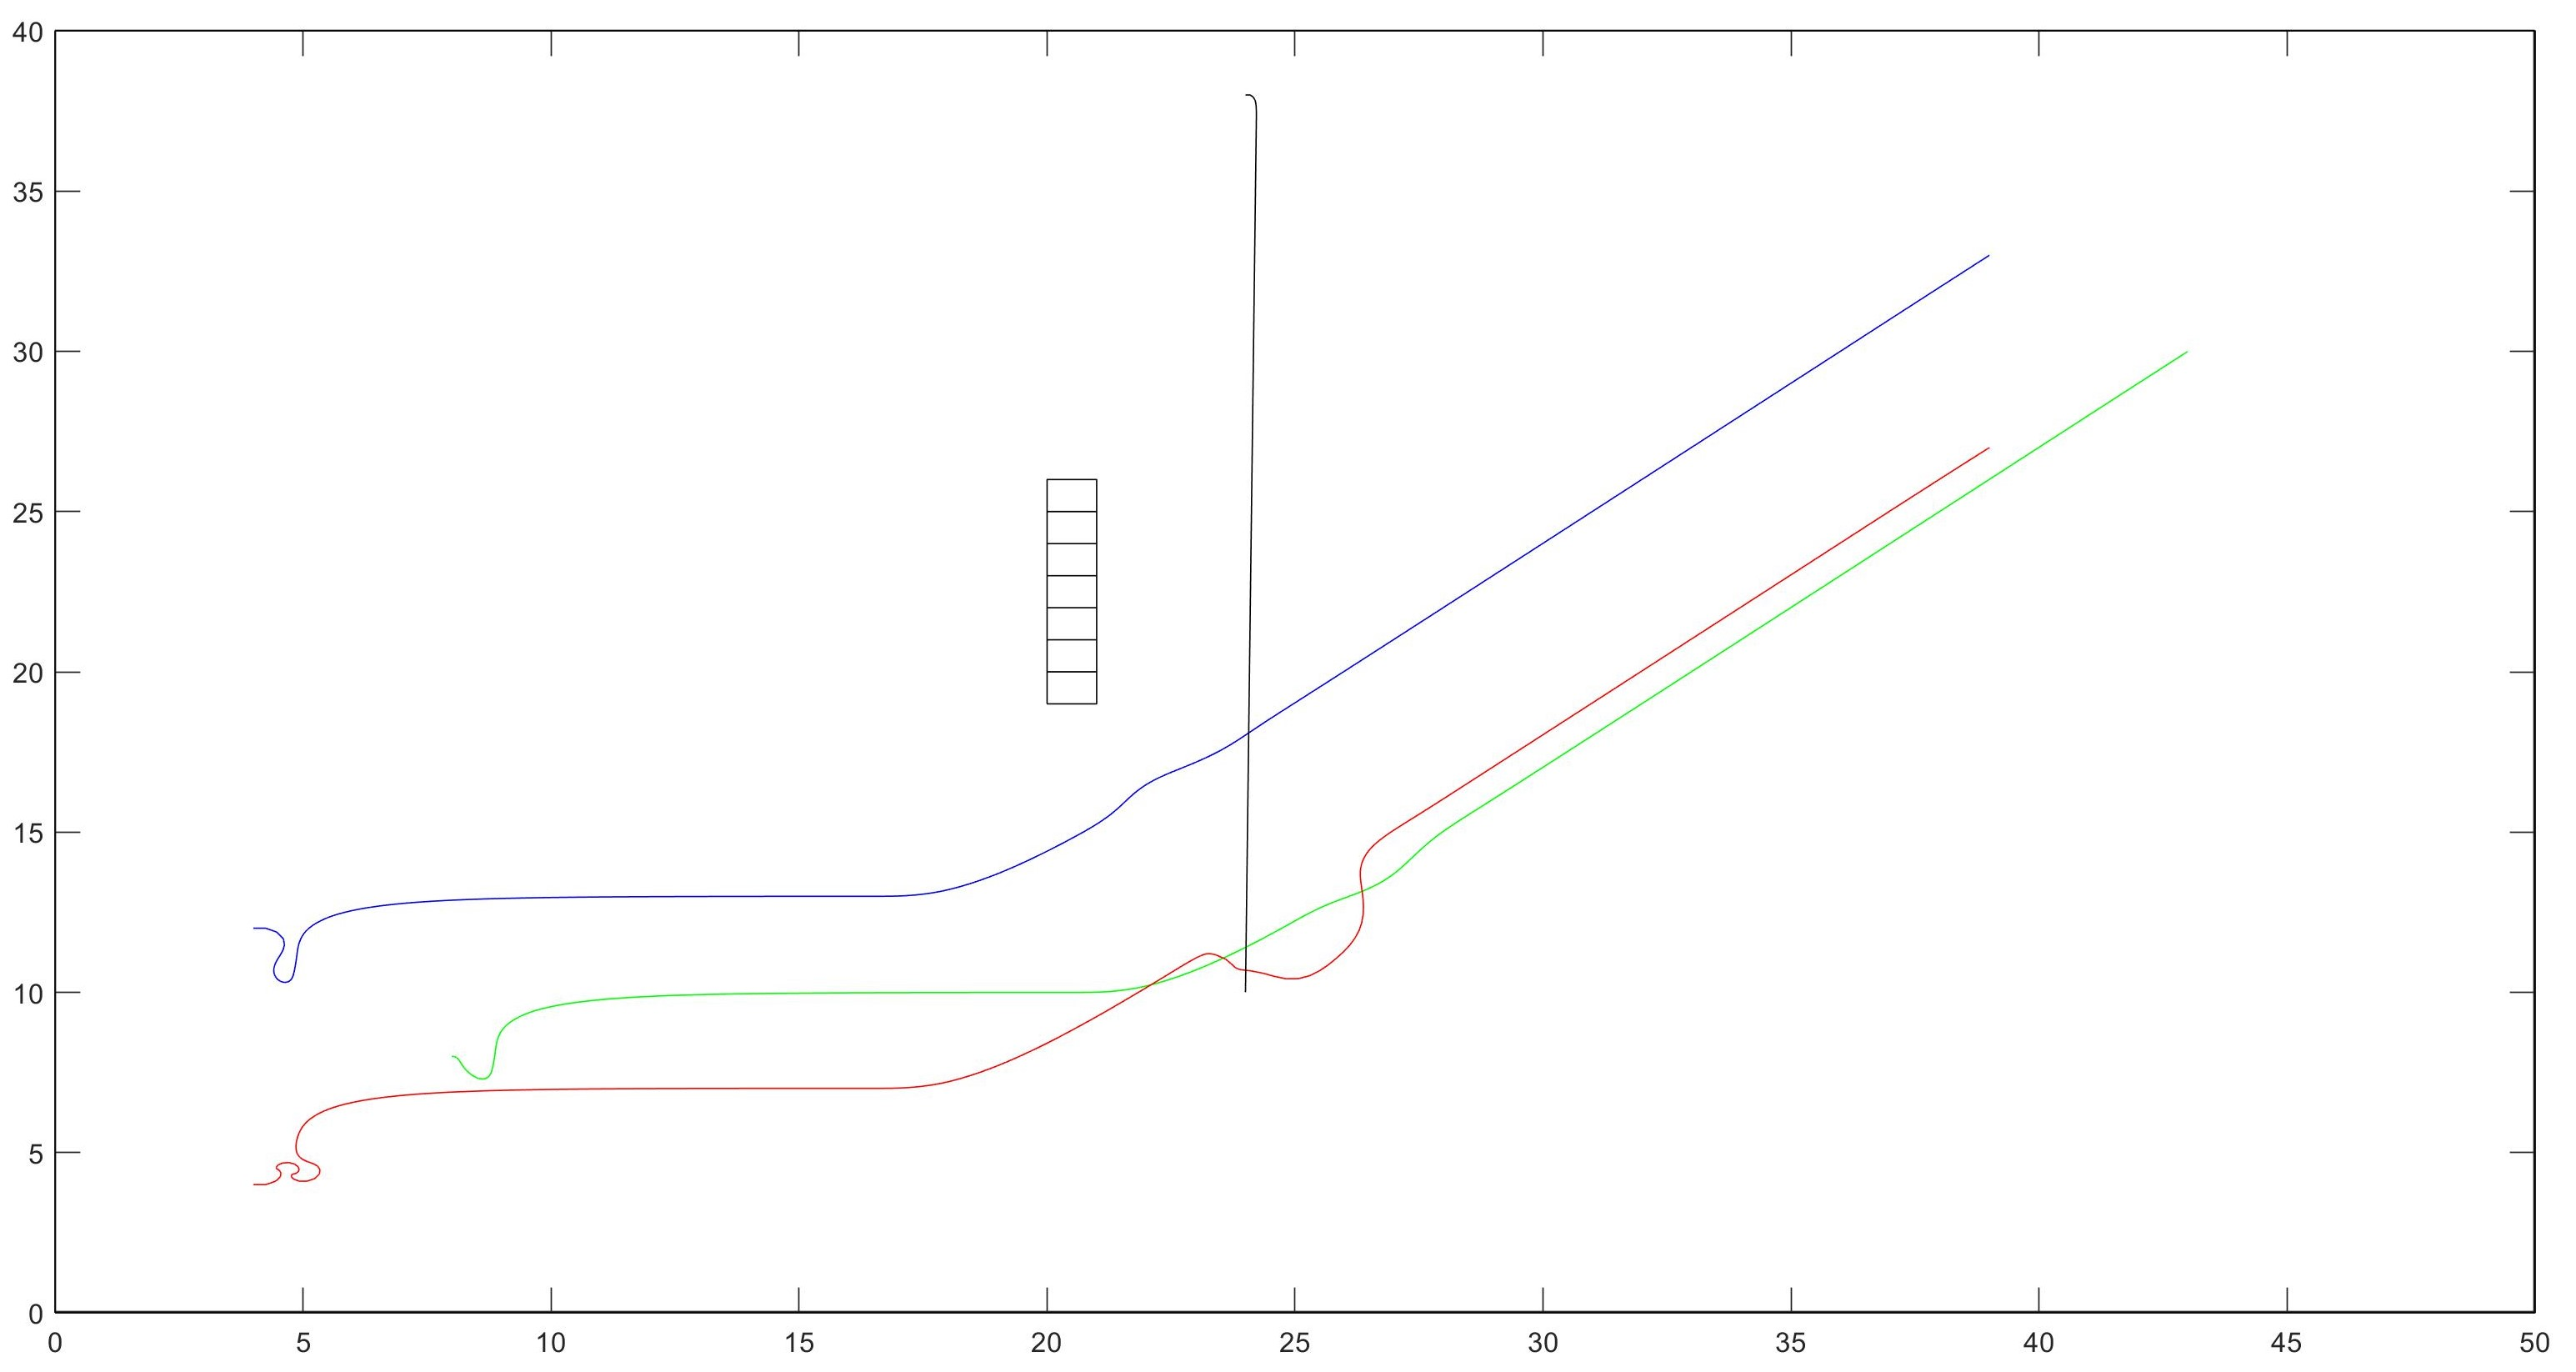
\includegraphics[scale=0.2]{Images/dynamic-potential-field.jpg}
	\caption{مکان ربات‌ها در روش میدان پتانسیل همراه با مانع متحرک}
\end{figure}

\begin{figure}[!h]
	\centering
	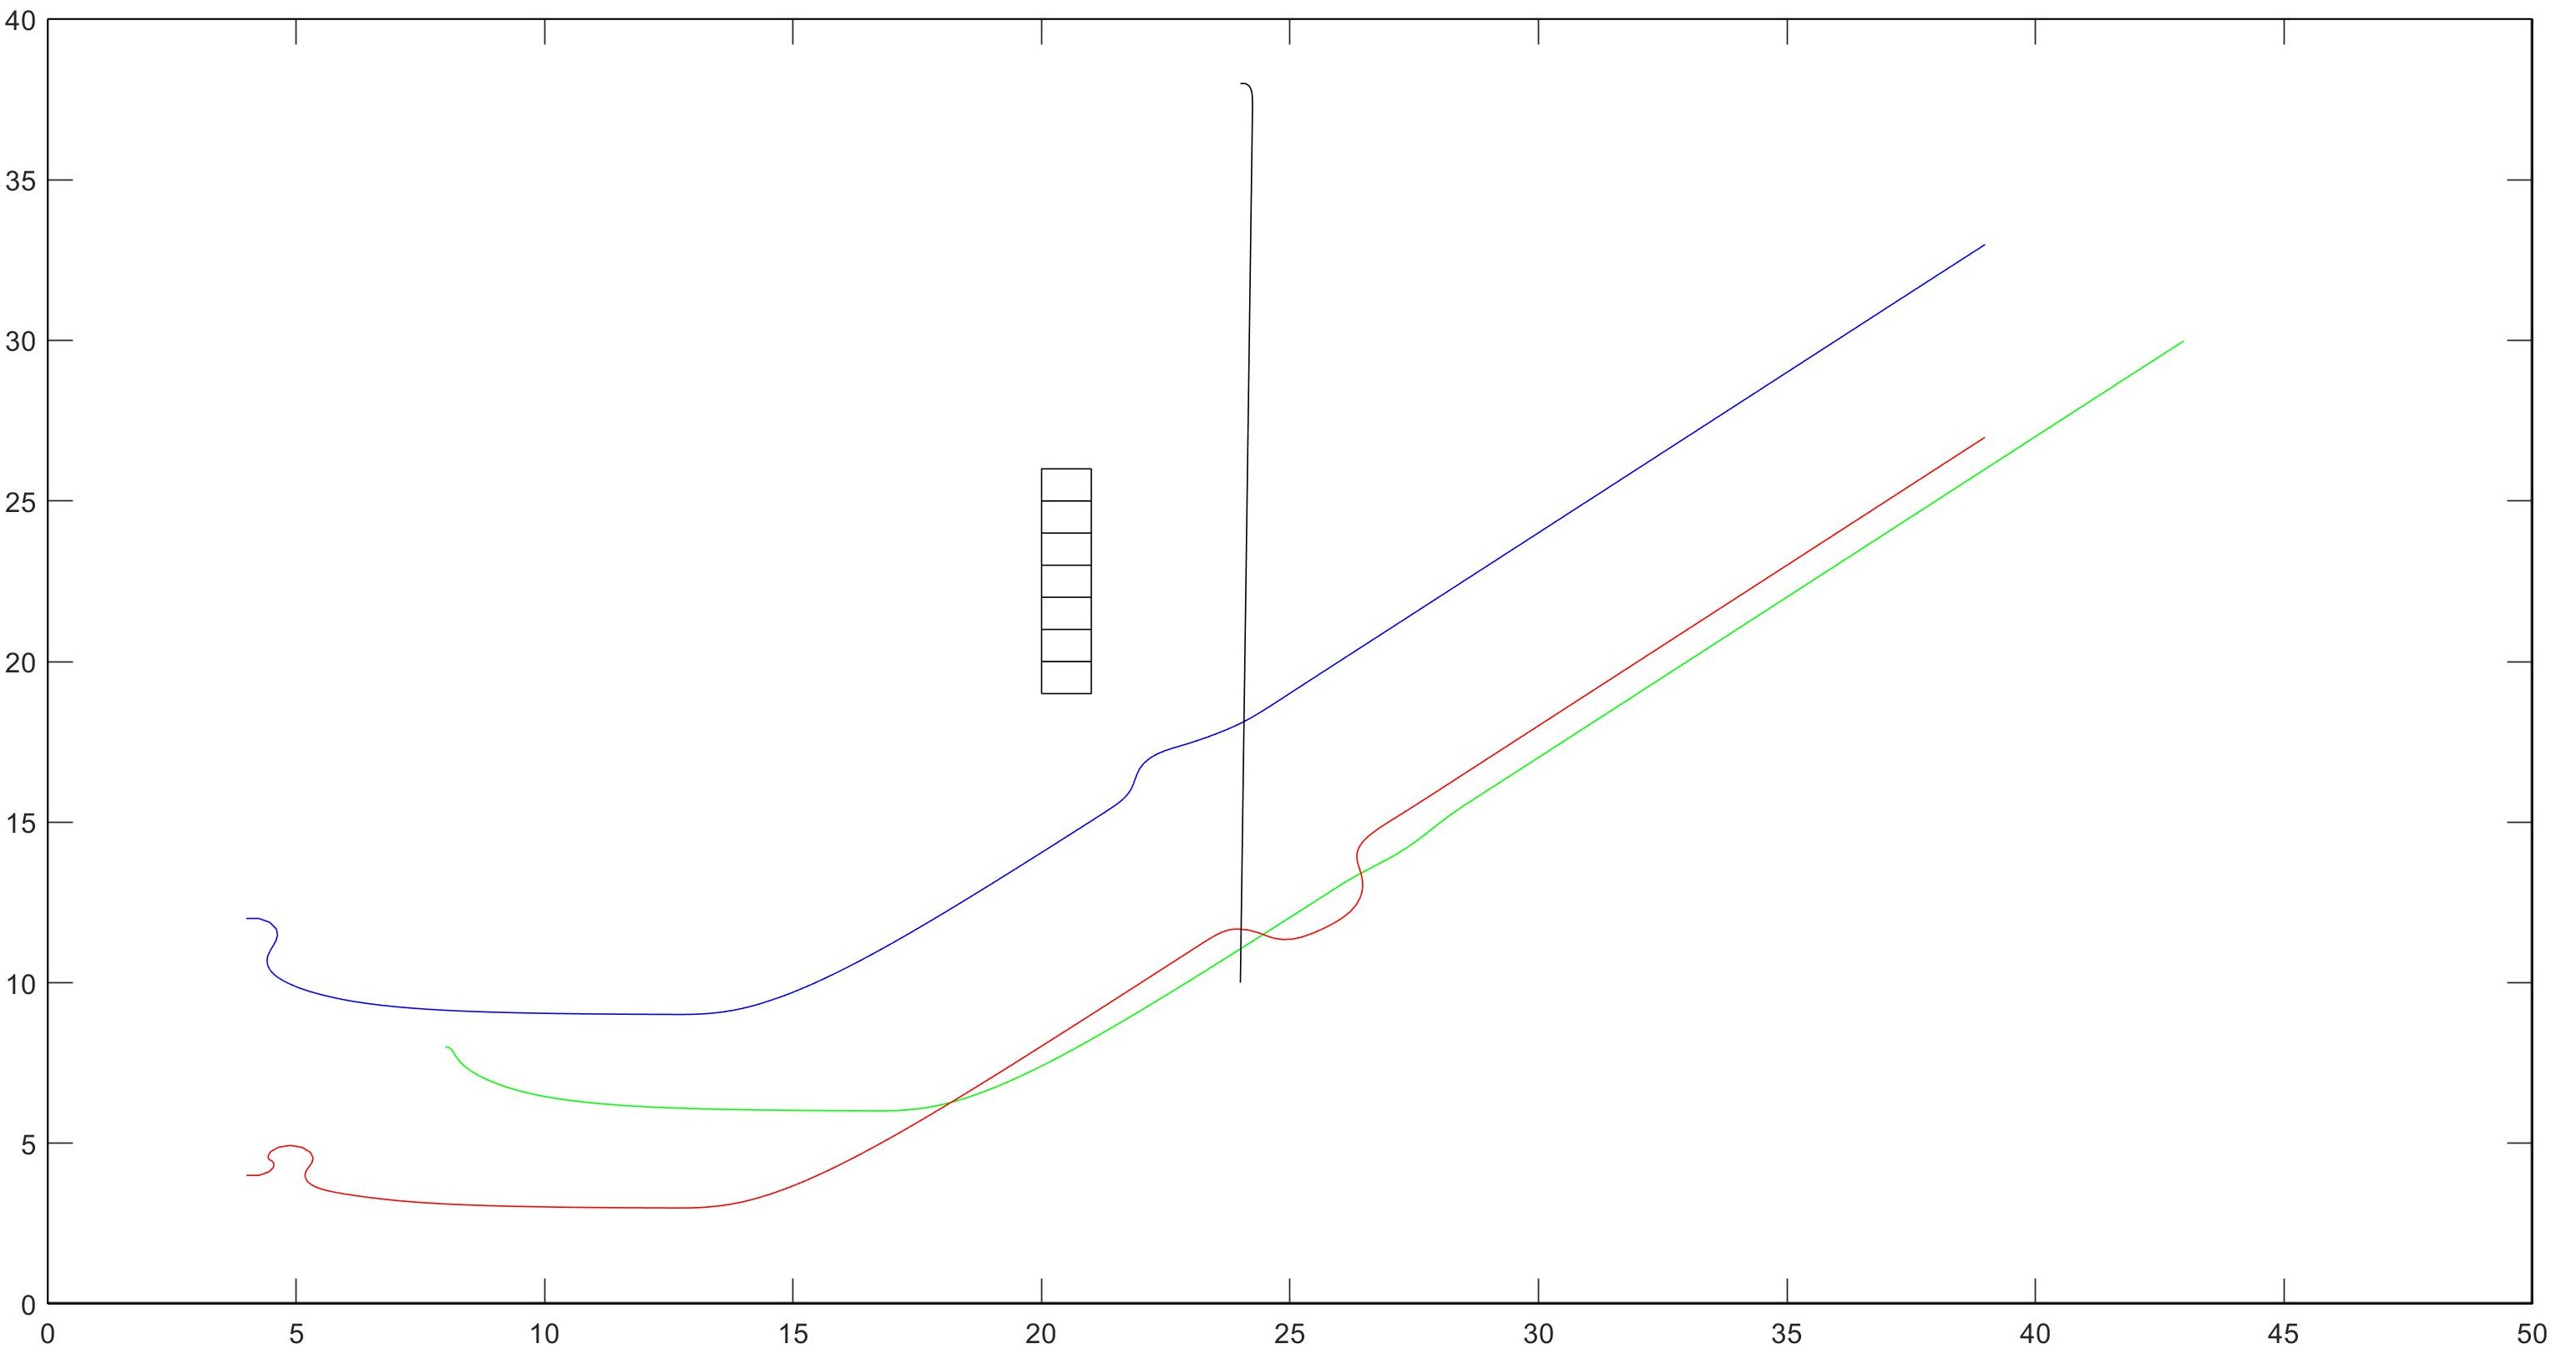
\includegraphics[scale=0.2]{Images/dynamic-BFS.jpg}
	\caption{مکان ربات‌ها در روش \lr{BFS} همراه با مانع متحرک}
\end{figure}

\begin{figure}[!h]
	\centering
	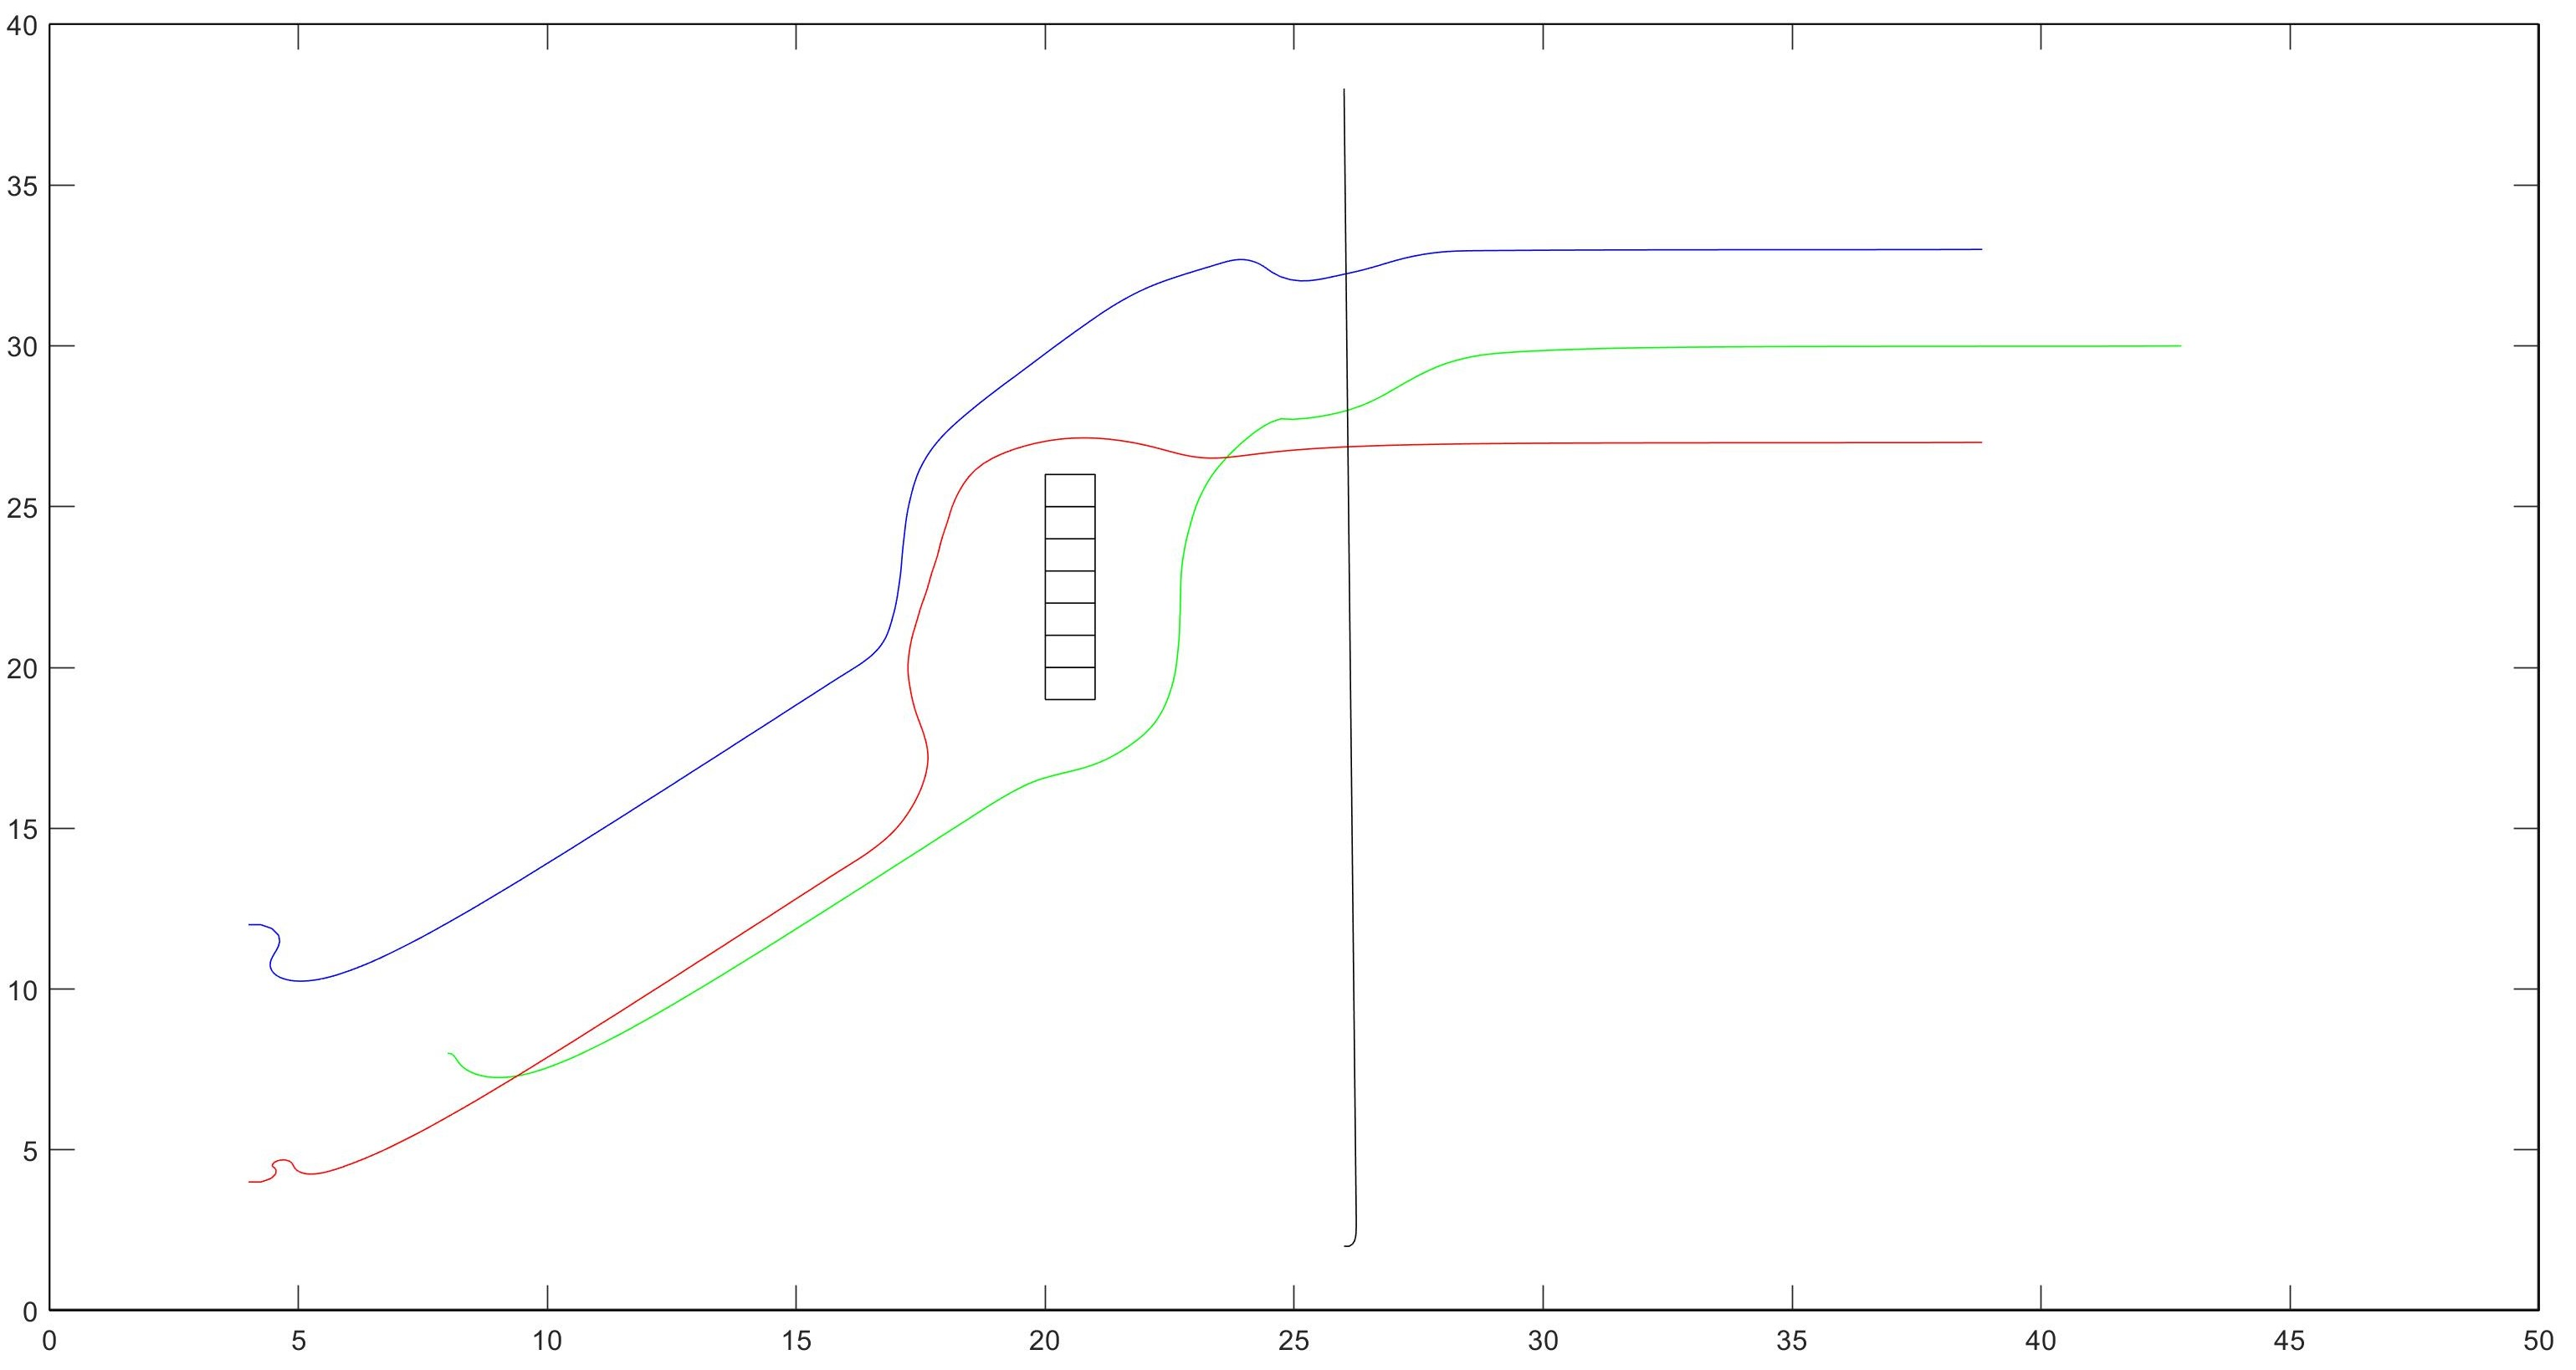
\includegraphics[scale=0.2]{Images/dynamic-Greedy.jpg}
	\caption{مکان ربات‌ها در روش \lr{Greedy best-first search} همراه با مانع متحرک}
\end{figure}

\begin{figure}[!h]
	\centering
	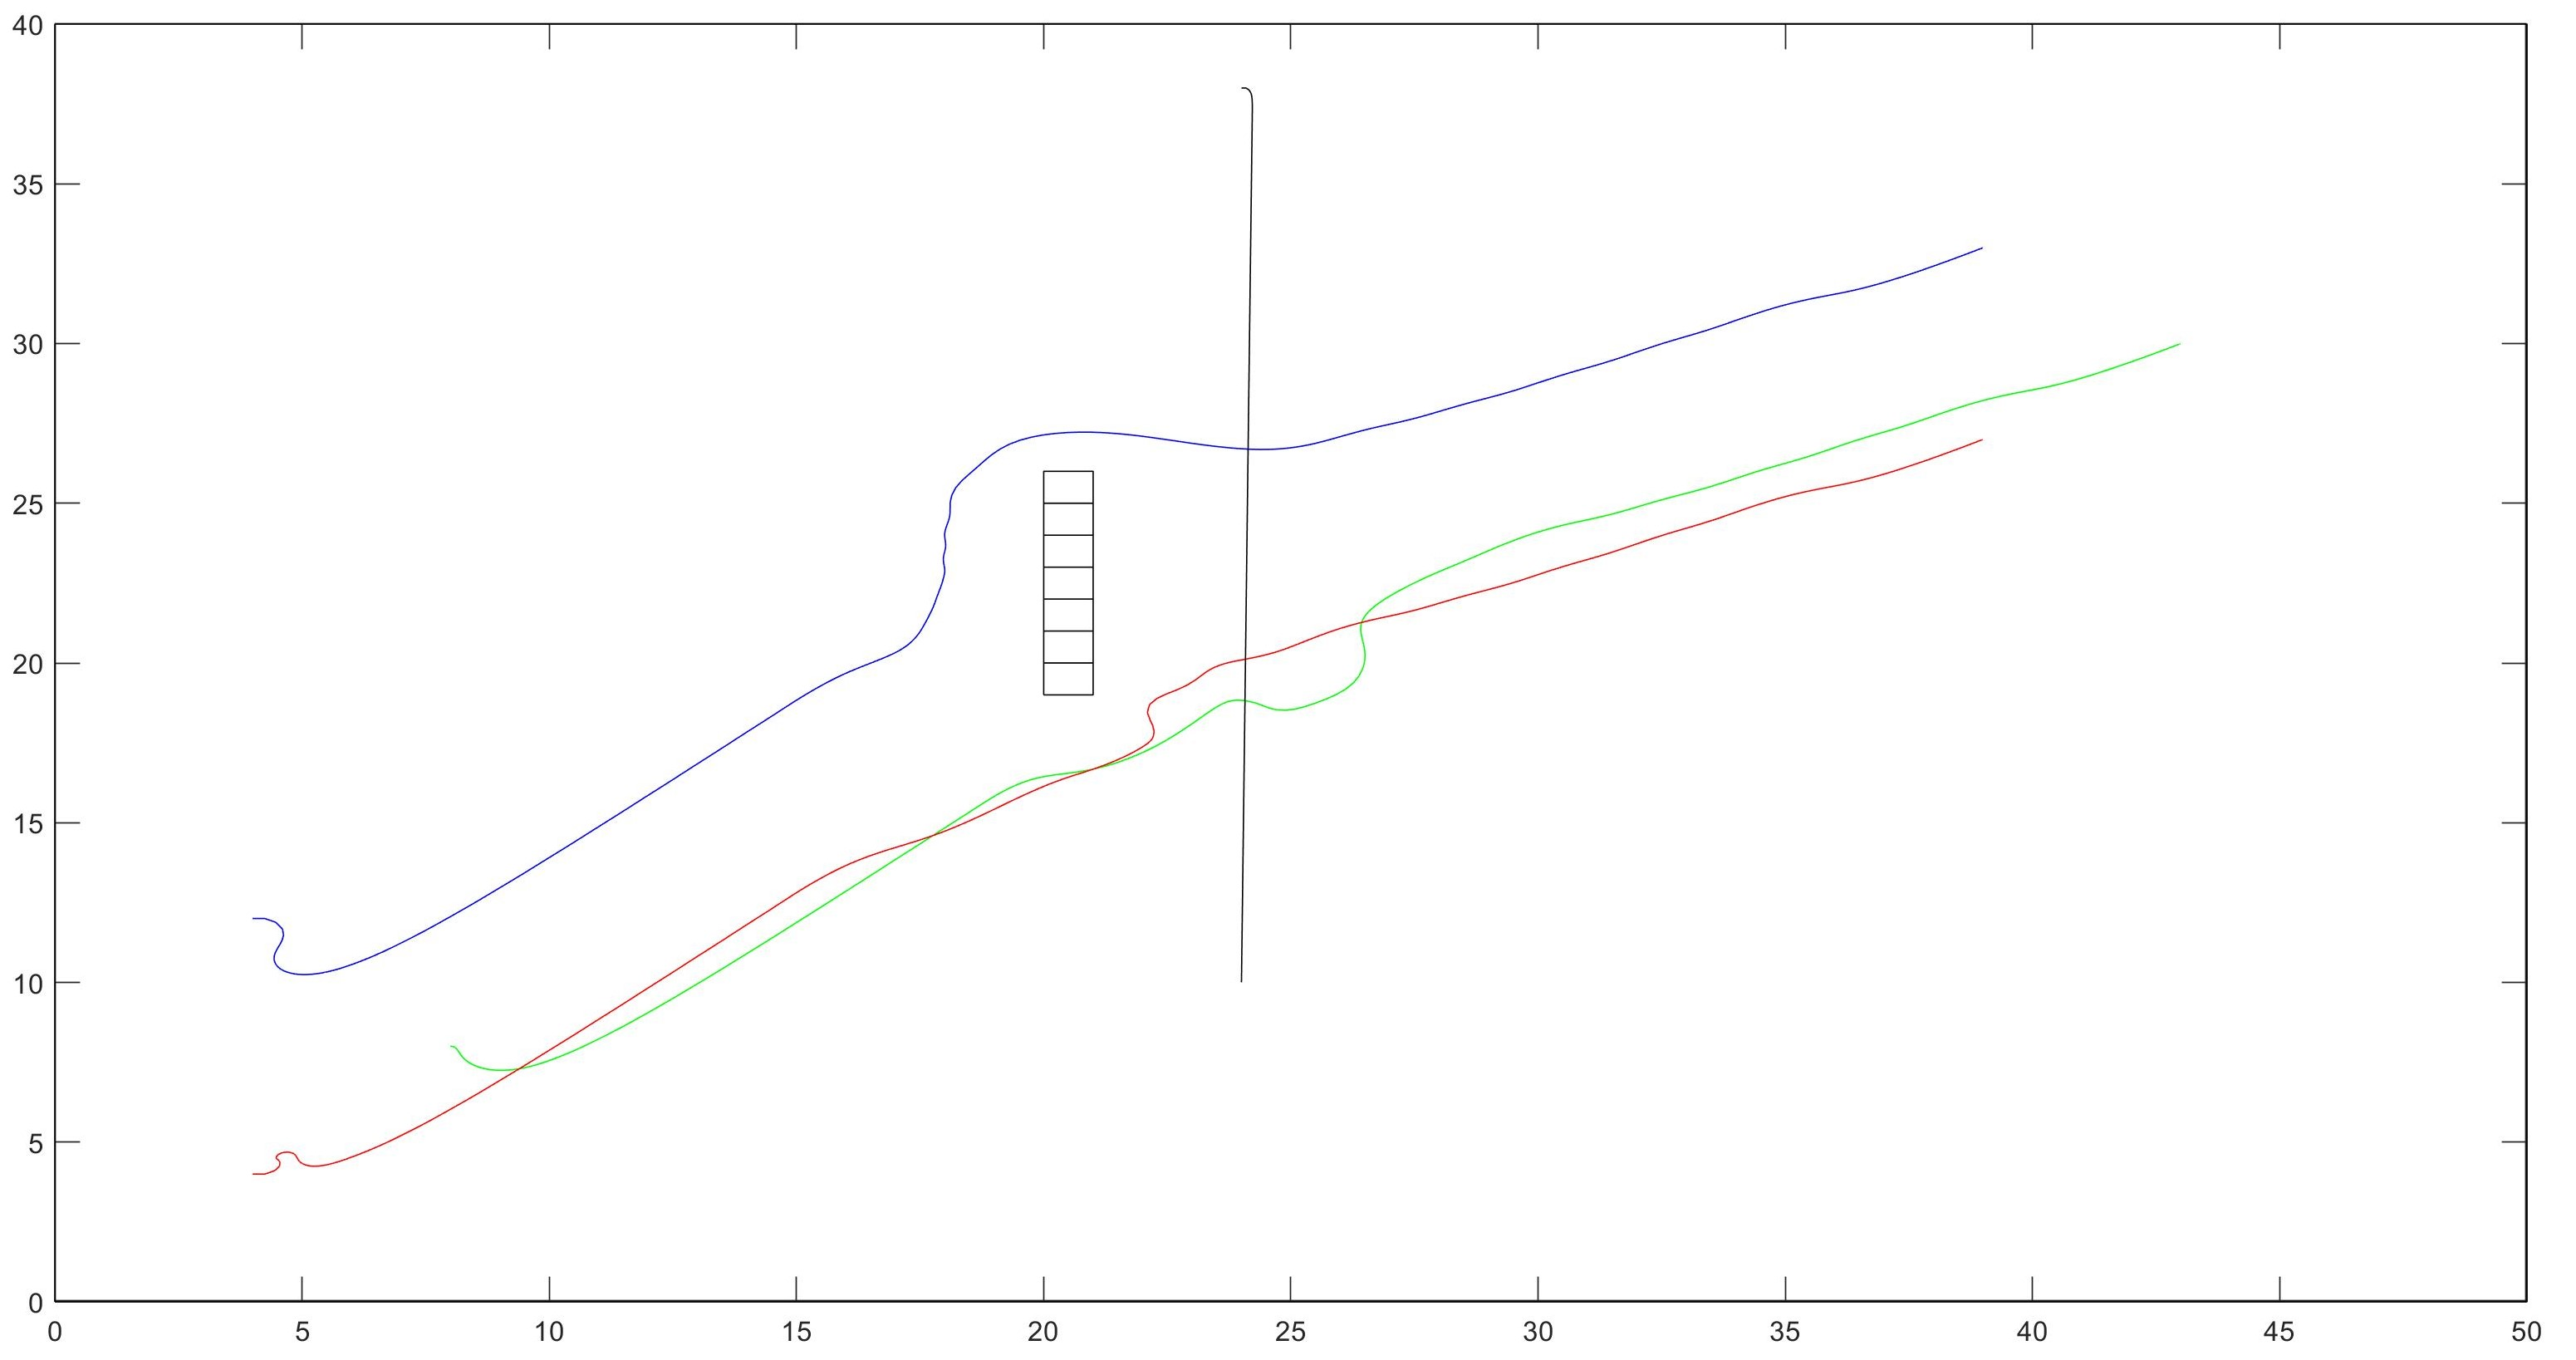
\includegraphics[scale=0.2]{Images/dynamic-A-star.jpg}
	\caption{مکان ربات‌ها در روش $A^*$ همراه با مانع متحرک}
\end{figure}









%--------------------------------------------------------------------------appendix( مراجع و پیوست ها)
\chapterfont{\vspace*{-2em}\centering\LARGE}%

\appendix
\bibliographystyle{plain-fa}
\bibliography{references}
\chapter*{‌پیوست}
\markboth{پیوست}{}
\addcontentsline{toc}{chapter}{پیوست}
موضوعات مرتبط با متن گزارش پایان نامه كه در يكی از گروه‌های زير قرار می‌گيرد، در بخش پيوست‌ها آورده شوند:
\begin{enumerate}
\item  اثبات های رياضی يا عمليات رياضی طولانی‌.‌
\item داده و اطلاعات نمونه (های) مورد مطالعه (\lr{Case Study}) چنانچه طولانی باشد‌.‌
\item نتايج كارهای ديگران چنانچه نياز به تفصيل باشد‌.‌
\item مجموعه تعاريف متغيرها و پارامترها، چنانچه طولانی بوده و در متن به انجام نرسيده باشد‌.‌
\end{enumerate}
% براي شماره‌گذاري روابط، جداول و اشكال موجود در پيوست‌ از ساختار متفاوتي نسبت به متن اصلي استفاده مي‌شود كه در زير به‌عنوان نمونه نمايش داده شده‌است. 
% \begin{equation}
%F=ma
%\end{equation}
\section*{کد میپل }
\begin{latin}
\begin{verbatim}

with(DifferentialGeometry):
with(Tensor):
DGsetup([x, y, z], M)
																	frame name: M
a := evalDG(D_x)
																	D_x
b := evalDG(-2 y z D_x+2 x D_y/z^3-D_z/z^2)


\end{verbatim}
\end{latin}
%--------------------------------------------------------------------------dictionary(واژه نامه ها)
%اگر مایل به داشتن صفحه واژه‌نامه نیستید، خط زیر را غیر فعال کنید.
\parindent=0pt
%
\chapter*{واژه‌نامه‌ی فارسی به انگلیسی}
\pagestyle{style9}

\addcontentsline{toc}{chapter}{واژه‌نامه‌ی فارسی به انگلیسی}
%%%%%%
\begin{multicols*}{2}

{\bf آ}
\vspace*{3mm}


\farsiTOenglish{اسکالر}{Scalar}


\vspace*{3mm}
{\bf ب}
\vspace*{3mm}

\farsiTOenglish{بالابر}{Lift}


\vspace*{3mm}
{\bf پ}
%%\vspace*{3mm}

\farsiTOenglish{پایا}{Invariant}



\vspace*{3mm}
{\bf ت}
%%\vspace*{3mm}

\farsiTOenglish{ تناظر }{Correspondence}


\vspace*{3mm}
{\bf ث}
%%\vspace*{3mm}

\farsiTOenglish{ثابت‌ساز}{Stabilizer}

\vspace*{3mm}
{\bf ج}
%%\vspace*{3mm}

\farsiTOenglish{جایگشت}{Permutation}



\vspace*{3mm}
{\bf چ}
%%\vspace*{3mm}


\farsiTOenglish{چند جمله‌ای }{Polynomial}

\vspace*{3mm}
{\bf ح}
%%\vspace*{3mm}

\farsiTOenglish{حاصل‌ضرب دکارتی}{Cartesian product}


\vspace*{3mm}
{\bf خ}
%%\vspace*{3mm}

\farsiTOenglish{خودریختی}{Automorphism}

\vspace*{3mm}
{\bf د}
%%\vspace*{3mm}

\farsiTOenglish{درجه}{Degree}


\vspace*{3mm}
{\bf ر}
%%\vspace*{3mm}


\farsiTOenglish{ریزپردازنده}{microprocessor}


\vspace*{3mm}
{\bf ز}
%%\vspace*{3mm}


\farsiTOenglish{زیرمدول}{Submodule}


\vspace*{3mm}
{\bf س}
%%\vspace*{3mm}

\farsiTOenglish{سرشت}{Character}


\vspace*{3mm}
{\bf ص}
%%\vspace*{3mm}

\farsiTOenglish{صادقانه}{Faithful}

\vspace*{3mm}
{\bf ض}
%%\vspace*{3mm}

\farsiTOenglish{ضرب داخلی}{Inner product}

\vspace*{3mm}
{\bf ط}
%%\vspace*{3mm}


\farsiTOenglish{طوقه}{Loop}


\vspace*{3mm}
{\bf ظ}
%%\vspace*{3mm}


\farsiTOenglish{ظرفیت}{Valency}
 
\vspace*{3mm}
{\bf ع}
%%\vspace*{3mm}


\farsiTOenglish{عدم مجاورت}{Nonadjacency}



\vspace*{3mm}
{\bf ف}
%%\vspace*{3mm}

\farsiTOenglish{فضای برداری}{Vector space}



\vspace*{3mm}
{\bf ک}
%%\vspace*{3mm}

\farsiTOenglish{کاملاً تحویل‌پذیر}{Complete reducibility}


\vspace*{3mm}
{\bf گ}
%%\vspace*{3mm}


\farsiTOenglish{گراف}{Graph}



\vspace*{3mm}
{\bf م}
%%\vspace*{3mm}

\farsiTOenglish{ماتریس جایگشتی}{Permutation matrix }


\vspace*{3mm}
{\bf ن}
%%\vspace*{3mm}

\farsiTOenglish{ناهمبند}{Disconnected}


\vspace*{3mm}
{\bf و}
%%\vspace*{3mm}

\farsiTOenglish{وارون‌پذیر}{Invertible}


\vspace*{3mm}
{\bf ه}
%%\vspace*{3mm}

\farsiTOenglish{همبند}{Connected}



\vspace*{3mm}
{\bf ی}
%%\vspace*{3mm}

\farsiTOenglish{یال}{Edge}




\end{multicols*}%
%%%%%%
\chapter*{ واژه‌نامه‌ی انگلیسی به فارسی}
\pagestyle{style9}
\lhead{\thepage}\rhead{واژه‌نامه‌ی انگلیسی به فارسی}
\addcontentsline{toc}{chapter}{واژه‌نامه‌ی انگلیسی به فارسی}

\LTRmulticolcolumns
\begin{multicols}{2}
{\hfill\bf  \lr{A}}
%%\vspace*{1.5mm}

\englishTOfarsi{Automorphism}{خودریختی}

\vspace*{3mm}
{\hfill\bf   \lr{B}}
%%\vspace*{1.5mm}

\englishTOfarsi{Bijection}{دوسویی}

\vspace*{3mm}
{\hfill\bf   \lr{C}}
%%\vspace*{1.5mm}

\englishTOfarsi{Cycle group}{گروه دوری}

\vspace*{3mm}
{\hfill\bf   \lr{D}}
%%\vspace*{1.5mm}

\englishTOfarsi{Degree}{درجه}

\vspace*{3mm}
{\hfill\bf   \lr{E}}
%%\vspace*{1.5mm}

\englishTOfarsi{Edge}{یال}

\vspace*{3mm}
{\hfill\bf   \lr{F}}
%%\vspace*{1.5mm}

\englishTOfarsi{Function}{تابع}

\vspace*{3mm}
{\hfill\bf   \lr{G}}
%%\vspace*{1.5mm}

\englishTOfarsi{Group}{گروه}

\vspace*{3mm}
{\hfill\bf   \lr{H}}
%%\vspace*{1.5mm}

\englishTOfarsi{Homomorphism}{همریختی}

\vspace*{3mm}
{\hfill\bf   \lr{I}}
%%\vspace*{1.5mm}

\englishTOfarsi{Invariant}{پایا}

\vspace*{3mm}
{\hfill\bf   \lr{L}}
%%\vspace*{1.5mm}

\englishTOfarsi{Lift}{بالابر}

\vspace*{3mm}
{\hfill\bf   \lr{M}}
%%\vspace*{1.5mm}

\englishTOfarsi{Module}{مدول}

\vspace*{3mm}
{\hfill\bf   \lr{N}}
%%\vspace*{1.5mm}

\englishTOfarsi{Natural map}{نگاشت طبیعی}

\vspace*{3mm}
{\hfill\bf   \lr{O}}
%%\vspace*{1.5mm}

\englishTOfarsi{One to One}{یک به یک}

\vspace*{3mm}
{\hfill\bf   \lr{P}}
%%\vspace*{1.5mm}

\englishTOfarsi{Permutation group}{گروه جایگشتی}

\vspace*{3mm}
{\hfill\bf   \lr{Q}}
%%\vspace*{1.5mm}

\englishTOfarsi{Quotient graph}{گراف خارج‌قسمتی}

 \vspace*{3mm}
{\hfill\bf   \lr{R}}
%%\vspace*{1.5mm}

\englishTOfarsi{Reducible}{تحویل پذیر}

\vspace*{3mm}
{\hfill\bf   \lr{S}}
%%\vspace*{1.5mm}

\englishTOfarsi{Sequence}{دنباله}

 \vspace*{3mm}
{\hfill\bf   \lr{T}}
%%\vspace*{1.5mm}

\englishTOfarsi{Trivial character}{سرشت بدیهی}

\vspace*{3mm}
{\hfill\bf   \lr{U}}
%%\vspace*{1.5mm}

\englishTOfarsi{Unique}{منحصربفرد}

\vspace*{3mm}
{\hfill\bf   \lr{V}}
%%\vspace*{1.5mm}

\englishTOfarsi{Vector space}{فضای برداری}
\end{multicols}
%--------------------------------------------------------------------------index(نمایه)
%اگر مایل به داشتن صفحه نمایه نیستید، خط زیر را غیر فعال کنید.
\pagestyle{style7}
\printindex
\pagestyle{style7}
%کلمات کلیدی انگلیسی
\latinkeywords{Write a 3 to 5 KeyWords is essential. Example: AUT, M.Sc., Ph. D,..}
%چکیده انگلیسی

\en-abstract{
This page is accurate translation from Persian abstract into English.
}
%%%%%%%%%%%%%%%%%%%%% کدهای زیر را تغییر ندهید.

\newpage
\thispagestyle{empty}
\begin{latin}
\section*{\LARGE\centering Abstract}

\een-abstract

\vspace*{.5cm}
{\large\textbf{Key Words:}}\par
\vspace*{.5cm}
\elatinkeywords
\end{latin}
% در این فایل، عنوان پایان‌نامه، مشخصات خود و چکیده پایان‌نامه را به انگلیسی، وارد کنید.
%%%%%%%%%%%%%%%%%%%%%%%%%%%%%%%%%%%%
\baselineskip=.6cm
\begin{latin}

\latinfaculty{Department of ...}


\latintitle{Title of Thesis}


\firstlatinsupervisor{Dr. }

%\secondlatinsupervisor{Second Supervisor}

\firstlatinadvisor{Dr. }

%\secondlatinadvisor{Second Advisor}

\latinname{Name}

\latinsurname{Surname}

\latinthesisdate{Month \& Year}

\latinvtitle
\end{latin}

\end{document}